\documentclass[print,gray]{dspbook}

\addbibresource{references.bib}
\newabbreviation{erm}{ERM}{empirical risk minimization}
\newabbreviation{svm}{SVM}{support vector machine}
\newabbreviation{bnf}{BNF}{Backus–Naur form}
\newabbreviation{sql}{SQL}{structured query language}
\newabbreviation{ibm}{IBM}{International Business Machines Corporation}
\newabbreviation{rdbms}{RDBMS}{relational database management system}
\newabbreviation{etl}{ETL}{extract, transform, load}
\newabbreviation{bi}{BI}{business intelligence}
\newabbreviation{hdfs}{HDFS}{hadoop distributed file system}
\newabbreviation{lusi}{LUSI}{learning using statistical inference}
\newabbreviation{iot}{IoT}{internet of things}
\newabbreviation{lifo}{LIFO}{last-in-first-out}
\newabbreviation{fifo}{FIFO}{first-in-first-out}
\newabbreviation{pmf}{PMF}{probability mass function}
\newabbreviation{pdf}{PDF}{probability density function}
\newabbreviation{cdf}{CDF}{cumulative distribution function}
\newabbreviation{cicd}{CI/CD}{continuous integration/continuous deployment}
\newabbreviation{slt}{SLT}{statistical learning theory}
\newabbreviation{ai}{AI}{artificial intelligence}
\newabbreviation{ml}{ML}{machine learning}
\newabbreviation{vc}{VC}{Vapnik-Chervonenkis}
\newabbreviation{srm}{SRM}{structural risk minimization}
\newabbreviation{mlp}{MLP}{multilayer perceptron}
\newabbreviation{iqr}{IQR}{interquartile range}
\newabbreviation{cnn}{CNN}{convolutional neural network}
\newabbreviation{pca}{PCA}{principal component analysis}

\newglossaryentry{ontology}{%
  name=ontology,
  description={%
    Ontology is the study of being, existence and reality. In computer science and
    information science, an ontology is a formal naming and definition of the types,
    properties, and interrelationships of the entities that really or fundamentally exist
    for a particular domain.}
}

\newglossaryentry{leakage}{%
  name=data leakage,
  description={%
    Situation where information from the test set is used to transform the training
    set in any way or to train the model.}
}

\newglossaryentry{model}{%
  name=model,
  description={%
    A general function that can be used to estimate the relationship between the
    input and output variables in a dataset.}
}

\newglossaryentry{preprocessor}{%
  name=preprocessor,
  description={%
    A chain of data handling operations that transforms the input data into a format that
    is suitable for the model.}
}

\makeglossaries


\title{Data Science Project: An Inductive Learning Approach}
\author{Filipe A. N. Verri}

\begin{document}

\setupfonts
\setuphyperref

\frontmatter

\thispagestyle{empty}
\begin{tikzpicture}[remember picture, overlay]
  \node[anchor=south east, inner sep=8mm] at (current page.south east) {%
    \reflectbox{\includegraphics[height=0.3\paperheight]{images/toucan_bw.png}}%
  };
  \node[anchor=south west, inner sep=10mm] at (current page.south west)
    {\large\sffamily Version 0.1 ``\textit{Audacious Hatchling}''};
    % {\large\sffamily Version 1.0 ``\textit{Tropical Toucan}''};
  \node[anchor=south east, inner sep=10mm] at (current page.south east) {\large\sffamily\today};
  \node[anchor=north, yshift=-25mm](title) at (current page.north) {\HUGE\sffamily\uppercase{Data Science Project}};
  \node[anchor=north, inner sep=5mm](subtitle) at (title.south) {\LARGE\sffamily\uppercase{An Inductive Learning Approach}};
  \node[anchor=north, inner sep=5mm] at (subtitle.south) {\Large\sffamily\uppercase{Filipe A. N. Verri}};
\end{tikzpicture}

\newpage
\thispagestyle{empty}
\phantom{foo}
\clearpage

\newpage

\thispagestyle{empty}
\begin{tikzpicture}[remember picture, overlay]
  \node[anchor=center] (logo) at (current page.center) {%
    
\includegraphics[height=0.3\paperheight]{images/zippi_bw.pdf}%
  };
  \node[anchor=south] (title) at (logo.north) {\large\sffamily This physical copy is offered to you by};
  \node[anchor=north] (subtitle) at (logo.south) {\large\sffamily\href{https://zippi.com.br/}{zippi.com.br}};
\end{tikzpicture}

\newpage

{
  \footnotesize\noindent Cite this book as:
  \begin{verbatim}
  @misc{verri2024datascienceproject,
    author = {Verri, Filipe Alves Neto},
    title = {Data Science Project: An Inductive Learning Approach},
    year = 2024,
    publisher = {Leanpub},
    version = {v0.1.0},
    doi = {10.5281/zenodo.14498011},
    url = {https://leanpub.com/dsp}
  }
  \end{verbatim}

  \noindent\fullcite{verri2024datascienceproject}.
}

\vfill

{
  \footnotesize\noindent
  \textbf{Disclaimer:} This book is a work in progress.  The print version may not be up
  to date with the latest changes.  The latest version is always available at
  \url{https://leanpub.com/dsp}.
}

\vspace{0.5cm}
{
\footnotesize\noindent
The book is typeset with \XeTeX{} using the Memoir class.  All figures are
original and created with Ti\textit{k}Z.  Proudly written in
\href{https://neovim.io/}{Neovim}.  \LaTeX{} code written with the assistance of
\href{https://github.com/features/copilot}{GitHub Copilot} and
\href{https://www.anthropic.com/claude-code}{Claude Code}.
All the text is original and not AI-generated.
The book cover image was created with the assistance of
\href{https://gemini.google.com}{Gemini} and \href{https://openai.com/dall-e-2}{DALL·E 2}.
We use the beautiful \href{https://www.stixfonts.org/}{STIX fonts} for text and math.
Some icons are from \href{https://fontawesome.com/}{Font Awesome 5} by Dave Gandy.
}

\vspace{0.5cm}
{
\footnotesize\noindent
Scripture quotations are from The ESV® Bible (The Holy Bible, English Standard Version®),
copyright © 2001 by Crossway, a publishing ministry of Good News Publishers. Used by
permission. All rights reserved.
}

\vspace{0.5cm}
{
\footnotesize\noindent
\thetitle{} © 2023--\the\year{} by \theauthor{}~\orcidlink{0000-0002-8240-5129} is licensed under
Attribution-NonCommercial-NoDerivatives 4.0 International. To view a copy of this license,
visit
\href{http://creativecommons.org/licenses/by-nc-nd/4.0/}{creativecommons.org/licenses/by-nc-nd/4.0}.
}

\cleardoublepage

\chapter{Foreword}

\chapterprecishere{\raggedleft\textup{by} \textsc{Ana Carolina Lorena}}

Data is now a ubiquitous presence and is collected every time and everywhere. However, the
real challenge lies in harnessing this data to generate actionable insights that guide
decision-making and drive innovation. This is the essence of data science, a
multidisciplinary field that leverages mathematical, statistical, and computational
techniques to analyse data and solve complex problems.

The book ``Data Science Project: An Inductive Learning Approach'' by F.A.N. Verri provides
readers with a structured and insightful exploration of the entire data science pipeline,
from the initial stages of data collection to the final step of model deployment. The book
effectively balances theory and practice, focusing on the inductive principles
underpinning predictive analytics and machine learning.

While other texts focus solely on machine learning algorithms or delve deeply into
tool-specific details, this book provides a holistic view of every stage of a data science
project. It emphasises the importance of robust data handling, sound statistical learning
principles, and meticulous model evaluation. The author thoughtfully integrates the
mathematical foundations and practical considerations needed to design and execute
successful data science projects.

Beyond the technical mechanics, this book challenges
readers to critically evaluate their models' strengths and limitations. It underscores the
importance of semantics in data handling, equipping readers with the skills to interpret
and transform data meaningfully.

\begin{sloppypar}
\emergencystretch=1em
Whether you are a student embarking on your first data science project or a data scientist
professional seeking to expand and refine your skills, this book's clarity, rigour, and
practical focus make it a guide that will serve you well in tackling the complex
challenges of data-driven decision-making. The book will expand your understanding and
inspire you to approach data science projects with a commitment to creating responsible
and impactful solutions.
\end{sloppypar}

% vim: spell spelllang=en


\cleardoublepage

\chapter{Preface}

\noindent Dear reader, \vspace{1em}

This book is based on the lecture notes from my course PO-235 Data Science Project, which
I teach to graduate students at both the Aeronautics Institute of Technology (ITA) and the
Federal University of São Paulo (UNIFESP) in Brazil.  I have been teaching this subject
since 2021, and I have continually updated the material each year.

Also, I was the coordinator of the Data Science Specialization Program (CEDS) at ITA.
That experience, which included a great deal of administrative work, as well as teaching and
supervising professionals in the course, has helped me to understand the needs of the
market and the students.

Moreover, parts of the project development methodology presented here came from my
experience as a lead data scientist in R\&D projects for the Brazilian Air Force,
which included projects in areas such as image processing, natural language processing,
and spatio-temporal data analysis.

Literature provides us with a wide range of excellent theoretical material on machine learning and
statistics, and highly regarded practical books on data science tools.  However, I missed
something that could provide a solid foundation on data science, covering all steps in a
data science project, including its software engineering aspects.

My goal is to provide a book that serves as a textbook for a course on data science
projects or as a reference for professionals working in the field.  I strive to maintain a
formal tone while preserving the practical aspects of the subject.  I do not focus on
a specific tool or programming language, but rather seek to explain the semantics of data
science tasks that can be implemented in any programming language.

Also, instead of teaching specific machine learning algorithms, I try to explain why
machine learning works, thereby increasing awareness of its pitfalls and limitations.
For this purpose, I assume you have a strong mathematical and statistical foundation.

One important artificial constraint I have imposed in the material (for the sake of the
course) is that I only consider predictive methods, more specifically inductive ones. I do
not address topics such as clustering, association rule mining, transductive learning,
anomaly detection, time series forecasting, reinforcement learning, etc.

I expect my approach on the subject to provide understanding of all steps in a data
science project, including a deeper focus on correct evaluation and validation of data
science solutions.

Note that, in this book, I openly express my opinions and beliefs. On several occasions it
may sound controversial.  I am not trying to be rude or to demean any researcher or
practitioner in the field; rather, I aim to be honest and transparent.

\vspace{1em}
\emph{I'd rather be bold and straightforward than cower about my beliefs.}
\vspace{1em}

I hope you enjoy reading.

\newpage

\begin{parwithqr}{https://github.com/verri/dsp-book}
  I intend to make this book forever free and open-source. You can find the source code at
  \href{\aurl}{github.com/verri/dsp-book}. Derivatives are not allowed, but you can
  contribute to the book. Contributors will be acknowledged here.
\end{parwithqr}

\vspace{3em}

\begin{lparwithqr}{https://leanpub.com/dsp}
  However, if you like this book, consider purchasing the e-book version at
  \href{\aurl}{leanpub.com/dsp}. Any amount you pay will help me keep this book updated
  and write new books.
\end{lparwithqr}

\vspace{3em}

\begin{parwithqr}{https://github.com/verri/dsp-book/discussions}
  If you have suggestions or questions, please open or join a discussion at
  \href{\aurl}{github.com/verri/dsp-book/discussions}. Feel free to ask anything.
  Theoretical discussions and practical advice are also welcome.
\end{parwithqr}

\vspace{3em}

\begin{lparwithqr}{https://www.buymeacoffee.com/verri}
  If you want to support me, you can \emph{buy me a coffee} at
  \href{\aurl}{buymeacoffee.com/verri}. I will greatly appreciate it.  I have a number of
  ideas for new books and courses, and financial support will enable me to make them a
  reality.
\end{lparwithqr}

\newpage

\section*{Contributors}

I would like to thank the following contributors for their help in improving this book:

\begin{itemize}
  \itemsep0em
  \item Johnny C. Marques
  \item Manoel V. Machado (aka \emph{ryukinix})
  \item Vitor V. Curtis
\end{itemize}

All contributors have freely waived their rights to the content they contributed to this book.

% vim: set spell spelllang=en:


\cleardoublepage

\tableofcontents

\cleardoublepage

\mainmatter

\chapter{A brief history of data science}
\label{chap:history}
\glsresetall

\chapterprecishere{``Begin at the beginning,'' the King said gravely, ``and
go on till you come to the end: then stop.''\par\raggedleft--- \textup{Lewis
Carroll}, Alice in Wonderland}

There are many points of view regarding the origin of data science.  For the sake of
contextualization, I separate the topic into two approaches: the history of the term itself
and a broad timeline of data-driven sciences, highlighting the important figures in each
age.

I believe that the history of the term is important for understanding the context of the
discipline. Over the years, the term has been employed to label quite different fields of
study.  Before presenting my view on the term, I present the views of two influential
figures in the history of data science: Peter Naur and William Cleveland.

Moreover, studying the key facts and figures in the history of data-driven sciences
enables us to comprehend the evolution of the field and hopefully guide us towards evolving it
further.  Besides, history also teaches us ways to avoid repeating the same mistakes.

Most of the significant theories and methods in data science have been developed
simultaneously across different fields, such as statistics, computer science, and engineering.
The history of data-driven sciences is long and rich. I present a timeline of the ages of
data handling and the most important milestones of data analysis.

I do not intend to provide a comprehensive history of data science.  I aim to provide
enough context to support the development of the material in the following chapters,
sometimes avoiding directions that are not relevant in the context of inductive learning.

\begin{mainbox}{Chapter remarks}

  \boxsubtitle{Contents}

  \startcontents[chapters]
  \printcontents[chapters]{}{1}{}
  \vspace{1em}

  \boxsubtitle{Context}

  \begin{itemize}
    \itemsep0em
    \item The term ``data science'' is recent and has been used to label rather different
      fields.
    \item The history of data-driven sciences is long and rich.
    \item Many important theories and methods in data science have been developed
      simultaneously in different fields.
    \item The history of data-driven sciences is important to understand the evolution of
      the field.
  \end{itemize}

  \boxsubtitle{Objectives}

  \begin{itemize}
    \itemsep0em
    \item Understand the history of the term ``data science.''
    \item Recognize the major milestones in the history of data-driven sciences.
    \item Identify important figures in the field of data-driven sciences.
  \end{itemize}

  \boxsubtitle{Takeaways}

  \begin{itemize}
    \itemsep0em
    \item We have evolved both in terms of theory and application of data-driven sciences.
    \item There is no consensus on the definition of data science (including which fields
      it encompasses).
    \item However, there is sufficient evidence to support data science as a distinct science.
  \end{itemize}
\end{mainbox}

{}
\clearpage

\section{The term ``data science''}

The term data science is relatively recent and has been used to label rather different fields of
study.  In the following, I emphasize the history of a few notable usages of the term.

\def\naurds{(0,0) circle (20mm)}
\def\naurcs{(0:5mm) circle (15mm)}
\def\naurde{(0:40mm) circle (15mm)}

\colorlet{circle edge}{black!50}
\colorlet{circle area}{black!20}

\tikzset{filled/.style={fill=circle area, draw=circle edge, thick},
    outline/.style={draw=circle edge, thick}}

\paragraph{Peter Naur (1928 -- 2016)}

The term ``data science'' itself was coined in the 1960s by Peter Naur (/naʊə/). Naur was
a Danish computer scientist and mathematician who made significant contributions to the
field of computer science, including his work on the development of programming
languages\footnote{He is best remembered as a contributor, with John Backus, to the
\gls{bnf} notation used in describing the syntax for most programming
languages.}.
His ideas and concepts laid the groundwork for the way we think about programming and data
processing today.

Naur disliked the term computer science and suggested it be called datalogy or data
science.  In the 1960s, the subject was practised in Denmark under Peter
Naur's term datalogy, which means the science of data and data processes.

He coined this term to emphasize the importance of data as a fundamental component of
computer science and to encourage a broader perspective on the field that included
data-related aspects. At that time, the field was primarily centered on programming
techniques, but Naur's concept broadened the scope to recognize the intrinsic role of data
in computation.

In his book\footfullcite{Naur1974}, ``Concise Survey of Computer Methods'', he
parts from the concept that \emph{data} is ``a representation of facts or ideas in a
formalised manner capable of being communicated or manipulated by some
process.''\footnote{I. H. Gould (ed.): ‘IFIP guide to concepts and terms in data
processing’, North-Holland Publ. Co., Amsterdam, 1971.} Note however that his view of the
science only ``deals with data [\dots] while the relation of data to what they represent
is delegated to other fields and sciences.''

\begin{figurebox}[label=fig:naur]{Naur's view of data science.}
  \centering
  \begin{tikzpicture}
    \begin{scope}
      \clip \naurds;
      \fill[filled] \naurcs;
    \end{scope}
    \draw[outline] \naurds node(ds) {};
    \draw[outline] \naurcs node {Computer science};
    \draw[outline] \naurde node {Domain expertise};
    \node[anchor=north,above] at (0,2) {Data science};
  \end{tikzpicture}
  \tcblower
    For Naur, data science studies the techniques to deal
    with data, but he delegates the meaning of data to other fields.
\end{figurebox}

It is interesting to see the central role he gave to data in the field of computer
science. His view that the relation of data to what they represent is delegated to other
fields and sciences is still debatable today.  Some scientists argue that data science
should focus on the techniques to deal with data, while others argue that data science
should encompass the whole business domain.  A depiction of Naur's view of data science is
shown in \cref{fig:naur}.

\def\clevelandds{(0,0) circle (20mm)}
\def\clevelandst{(0:-5mm) circle (15mm)}
\def\clevelandde {(2,1) circle (15mm)}
\def\clevelandcs {(2,-1) circle (15mm)}

\paragraph{William Cleveland (born 1943)}

In 2001, a prominent statistician used the term ``data science'' in his work to describe a
new discipline that comes from his ``plan to enlarge the major areas of technical work of
the field of statistics\footfullcite{Cleveland2001}.''
In 2014, that work was republished\footnote{W. S. Cleveland.
Data Science: An Action Plan for the Field of Statistics. Statistical Analysis and Data
Mining, 7:414–417, 2014. reprinting of 2001 article in ISI Review, Vol 69.}.
He advocates the expansion of statistics beyond theory into technical areas, significantly
changing statistics.  Thus, it warranted a new name.

As a result, William Swain Cleveland II is credited with defining data science as it is most
used today. He is a highly influential figure in the fields of statistics, machine
learning, data visualization, data analysis for multidisciplinary studies, and high
performance computing for deep data analysis.

\begin{figurebox}[label=fig:cleveland]{Cleveland's view of data science.}
  \centering
  \begin{tikzpicture}
    \begin{scope}
      \clip \clevelandds;
      \fill[filled] \clevelandst;
      \fill[filled] \clevelandde;
      \fill[filled] \clevelandcs;
    \end{scope}
    \draw[outline] \clevelandds node(ds) {};
    \draw[outline] \clevelandst node {Statistics};
    \draw[outline] \clevelandde node {Domain expertise};
    \draw[outline] \clevelandcs node {Computer science};
    \node[anchor=north,above] at (0,2) {Data science};
  \end{tikzpicture}
  \tcblower
    For Cleveland, data science is the ``modern'' statistics,
    where it is enlarged by computer science and domain expertise.
\end{figurebox}

In his view, data science is the ``modern'' statistics, where it is enlarged by computer
science methods and domain expertise.  An illustration of Cleveland's view of data science
is shown in \cref{fig:cleveland}.  It is important to note that Cleveland never defined an
explicit list of computer science fields and business domains that should be included in
the new discipline.  The main idea is that statistics should rely on computational methods
and that the domain expertise should be considered in the analysis.

\paragraph{Buzzword or a new science?}

Be aware that scientific literature has no consensus on the definition of data science, and it is still considered
by some to be a buzzword\footnote{Press, Gil. ``Data Science: What's The Half-Life of a
Buzzword?''. Forbes. Available at
\href{https://www.forbes.com/sites/gilpress/2013/08/19/data-science-whats-the-half-life-of-a-buzzword/}%
  {forbes.com/sites/gilpress/2013/08/19/data-science-whats-the-half-life-of-a-buzzword}.}.

Most of the usages of the term in literature and in the media are either a rough
reference to a set of data-driven techniques or a marketing strategy.  Naur
(\cref{fig:naur}) and Cleveland (\cref{fig:cleveland}) are among the few that try to
carefully define the term.  However, both of them do not see data science as an
independent field of study, but rather an enlarged scope of an existing science.  I disagree;
the social and economic demand for data-driven solutions has led to an evolution in our
understanding of the challenges we are facing.  As a result, we see many ``data
scientists'' being hired and many ``data science degree'' programs emerging.

In \cref{chap:data}, I dare to provide a (yet another) definition for the term.  I
argue that its object of study can be precisely established to support it as a new
science.

\section{Timeline and historical markers}

\textcite{Kelleher2018}\footfullcite{Kelleher2018} provides an interesting timeline of data-driven methods and
influential figures in the field.  I reproduce it here with some changes, including
some omissions and additions.  On the subject of data analysis, I include some
exceptional remarks
from \textcite{Vapnik1999b}\footfullcite{Vapnik1999b}.

I first address data handling --- which includes data sources, collection, organization,
storage, and transformation ---, and then data analysis and knowledge extraction.

\subsection{Timeline of data handling}
\label{sub:time-handling}

The importance of collecting and organizing data goes without saying.  Data fuels analysis and
decision making.  In the following, I present some of the most important milestones in the history
of data handling.

\begin{figurebox}[label=fig:data-handling-history]{Timeline of the ages of data handling.}
  \centering
  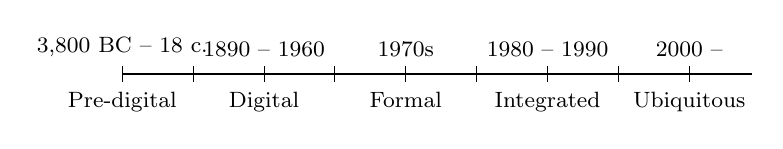
\begin{tikzpicture}
    \draw (0,0) -- (8,0);
    \foreach \x in {0,1,...,8} {
      \draw (0.9 * \x,-0.1) -- (0.9 * \x,0.1);
    }
    \foreach \x/\y/\z in {%
        0/Pre-digital/{3,800 BC -- \nth{18} c.},
        2/Digital/{1890 -- 1960},
        4/Formal/{1970s},
        6/Integrated/{1980 -- 1990},
        8/Ubiquitous/{2000 --}} {
      \node[anchor=north] at (0.9 * \x,-0.1) {\footnotesize\y};
      \node[anchor=south] at (0.9 * \x,0.1) {\footnotesize\z};
    }
  \end{tikzpicture}
\end{figurebox}

\Cref{fig:data-handling-history} illustrates the proposed timeline.  Ages have no absolute
boundaries, but rather periods where some important events happened.  Also, observe that
the timescale is not linear.  The Pre-digital Age is the longest period, and one could
divide it into smaller periods.  My choices of ages and their boundaries are motivated by
didactic reasons.

\subsubsection{Pre-digital age}

We can consider the earliest records of data collection to be the notches on sticks and
bones (probably) used to keep track of the passing of time.  The Lebombo bone, a baboon fibula with
notches, is one of the earliest known mathematical objects.  It was found in the Lebombo
Mountains located between South Africa and Eswatini.
They estimate it is more
than 40,000 years old. It is conjectured to be a tally stick, but its exact purpose is
unknown. Its 29 notches suggest that it may have been used as a lunar phase counter.
However, since it is broken at one end, the 29 notches may or may not be the total
number\footfullcite{Beaumont2013}.

Another milestone in the history of data collection is the record of
demographic data.  One of the first known censuses was conducted in 3,800 BC in the Babylonian
Empire.  It was ordered to assess the population and resources of
the empire.  Records were stored on clay tiles\footfullcite{Grajalez2013}.

Since the early forms of writing, humanity's abilities to register data and events
increased significantly.  The first known written records date back to around 3,500 BC, the
Sumerian archaic (pre-cuneiform) writing.  This writing system was used to represent
commodities using clay tokens and to record transactions\footfullcite{Ifrah1998}.

``Data storage'' was also a challenge.  Some important devices that increased our capacity
to register textual information are the Sumerian clay tablets (3,500 BC), the Egyptian
papyrus (3,000 BC), the Roman wax tablets (100 BC), the codex
(100 AD), the Chinese paper (200 AD), the printing press (1440), and the typewriter (1868).

% Talvez citar na parte de análise de dados
% Other mechanisms were also developed to store information in a more structured way.  Some
% important devices are
% the abacus (2,700 BC), the Antikythera mechanism (150 -- 100 BC), the
% Chinese South Pointing Chariot (260 AD), the Pascaline (1642), the Jacquard loom (1801),
% the Babbage Difference Engine (1822), the Babbage Analytical Engine (1837).

Besides those improvements in unstructured data storage, at least in the Western and
Middle Eastern world, there are no significant advances in structured data collection
until the \nth{19} century.  (An Eastern timeline research seems much harder to perform.
Unfortunately, I left it out in this book.)

I consider a major influential figure in the history of data
collection to be Florence Nightingale (1820 -- 1910).  She was a passionate statistician
and probably the first person to use statistics to influence public and official
opinion.  The meticulous records she kept during the Crimean War
(1853 -- 1856) were the evidence that saved lives --- part of the mortality came from lack
of sanitation.  She was also the first to use
statistical graphics to present data in a way that was easy to understand.  She is
credited with developing a form of the pie chart now known as the polar area
diagram.  She also reformed healthcare in the United Kingdom and
is considered the founder of modern nursing; where a great part of the work was to collect
data in a standardized way to quickly draw conclusions\footfullcite{Grajalez2013}.

\subsubsection{Digital age}

In the modern period, several devices were developed to store digital\footnote{Digital
means the representation of information in (finite) discrete form.  The term comes from the Latin
digitus, meaning finger, because it is the natural way to count using fingers.  Digital
here does not mean electronic.}
information.  One particular device that is important for data collection is the punched
card.  It is a piece of stiff paper that contains digital information represented by the
presence or absence of holes in predefined positions.  The information can be read by a
mechanical or electrical device called a card reader.  The earliest famous usage of
punched cards was by Basile Bouchon (1725) to control looms.  Most of the advances until
the 1880s were about the automation of machines (data processing) using hand-punched cards, and not
particularly specialized for data collection.

However, the 1890 census in the United States was the first to use machine-readable
punched cards to tabulate data. Processing 1880 census data took eight years, so the
Census Bureau contracted Herman Hollerith (1860 -- 1929) to design and build a tabulating
machine.  He founded the Tabulating Machine Company in 1896, which later merged with other
companies to become \gls{ibm} in 1924. Later
models of the tabulating machine were widely used for business applications such as
accounting and inventory control. Punched card technology remained a prevalent method of
data processing for several decades until more advanced electronic computers were
developed in the mid-\nth{20} century.

The invention of the digital computer is responsible for a revolution in data handling.
The amount of information we can capture and store increased exponentially.  ENIAC (1945) was
the first electronic general-purpose computer.  It was Turing-complete, digital, and
capable of being reprogrammed to solve a full range of computing problems.
It had 20 words of internal memory, each capable of storing a 10-digit decimal integer number.
Programs and data were entered by setting switches and inserting punched cards.

For the 1950 census, the United States Census Bureau used the
UNIVAC I (Universal Automatic Computer I), the first commercially produced computer in the
United States\footnote{Read more in \url{https://www.census.gov/history/www/innovations/}.}.

It goes without saying that digital computers have become much more powerful and
sophisticated since then.  The data collection process has been easily automated and
scaled to a level that was unimaginable before.  However, ``where'' storing data is
not the only challenge.  ``How'' to store data is also a challenge.  The next period of
history addresses this issue.

\subsubsection{Formal age}

In 1970, Edgar Frank Codd (1923 -- 2003), a British computer scientist,
published a paper entitled ``A Relational Model
of Data for Large Shared Data Banks''\footfullcite{Codd1970}.  In this paper, he introduced
the concept of a relational model for database management.

A relational model organizes data in tables (relations) where each row represents a record
and each column represents an attribute of the record.  The tables are related by common
fields.  Codd showed means to organize the tables of a relational database to minimize
data redundancy and improve data integrity.  \Cref{sec:normalization} provides more details
on the topic.

His work was a breakthrough in the field of data management.  The standardization of
relational databases led to the development of \gls{sql} in 1974.
SQL is a domain-specific language used in programming and designed for managing data held
in a \gls{rdbms}.

As a result, a new challenge rapidly emerged: how to aggregate data from different
sources. Once data is stored in a relational database, it is easy to query and manage
it. However, data is usually stored in different databases, and it is not always possible
to directly combine them.

\subsubsection{Integrated age}

The solution to this problem was the development of the \gls{etl}
process.  \gls{etl} is a process in data warehousing responsible for extracting data from
several sources, transforming it into a format that can be analyzed, and loading it into a
data warehouse.

The concept of data warehousing dates back to the late 1980s when IBM researchers Barry
Devlin and Paul Murphy developed the ``business data warehouse.''

Two major figures in the history of \gls{etl} are Ralph Kimball (born 1944) and Bill Inmon (born
1945), both American computer scientists.  Although they
differ in their approaches, they both agree that data warehousing is the foundation for
\gls{bi} and analytics, and that data warehouses should be designed to
be easy to understand and fast to query for business users.

A famous debate between Kimball and Inmon is the top-down versus bottom-up approach to
data warehousing.  Inmon's approach is top-down, where the data warehouse is designed
first and then the data marts\footnote{A data mart is a specialized subset of a data
warehouse that is designed to serve the needs of a specific business unit, department, or
functional area within an organization.} are created from the data warehouse.  Kimball's
approach is bottom-up, where the data marts are created first and then the data warehouse
is created from the data marts.

One of the earliest and most famous case studies of the implementation of a data warehouse
is that of Walmart. In the early 1990s, Walmart faced the challenge of managing and
analyzing vast amounts of data from its stores across the United States. The company
needed a solution that would enable comprehensive reporting and analysis to support
decision-making processes.  The solution was to implement a data warehouse that would
integrate data from various sources and provide a single source of truth for the
organization.

\subsubsection{Ubiquitous age}

The last and current period of history is the ubiquitous age.  It is characterized by the
proliferation of data sources.

The ubiquity of data generation and the evolution of data-centric technologies have been
made possible by a multitude of figures across various domains.

\begin{itemize}
  \itemsep0em
  \item Vinton Gray Cerf (born 1943) and Robert Elliot Kahn (born 1938), often referred to
    as the ``Fathers of the Internet,'' developed the TCP/IP protocols, which are
    fundamental to internet communication.
  \item Tim Berners-Lee (born 1955), credited with inventing the World Wide Web, laid the
    foundation for the massive data flow on the internet.
  \item Steven Paul Jobs (1955 -- 2011) and Stephen Wozniak (born 1950), from Apple Inc.,
    and William Henry Gates III (born 1955), from Microsoft Corporation, were responsible
    for the introduction of personal computers, leading to the democratization of data
    generation.
  \item Lawrence Edward Page (born 1973) and Sergey Mikhailovich Brin (born 1973), the
    founders of Google, transformed how we access and search for information.
  \item Mark Elliot Zuckerberg (born 1984), the co-founder of Facebook, played a crucial
    role in the rise of social media and the generation of vast amounts of user-generated
    content.
\end{itemize}

In terms of data handling, this change of landscape has brought about the
development of new technologies and techniques for data storage and processing.  Especially
the development of NoSQL databases and distributed computing frameworks.

NoSQL databases are non-relational databases that can store and process large volumes of
unstructured, semi-structured, and structured data.  They are highly scalable and
flexible, making them ideal for big data applications.

Some authors argue that the rise of big data is characterized by the five V's of big data:
Volume, Velocity, Variety, Veracity, and Value.  The amount of data generated is massive,
the speed at which data is generated is high, the types of data generated are diverse, the
quality of data generated is questionable, and the value of data generated is high.

Once massive amounts of unstructured data became available, the need for new data
processing techniques arose.  The development of distributed computing frameworks such as
Apache Hadoop and Apache Spark enabled the processing of massive amounts of data in a
distributed manner.

Douglass Read Cutting and Michael Cafarella, the developers of the software Apache Hadoop,
proposed both the \gls{hdfs} and MapReduce, which are the
cornerstones of the Hadoop framework, in 2006.  Hadoop's distributed storage and
processing capabilities enabled organizations to handle and analyze massive volumes of
data.

Currently, Google holds a patent for
MapReduce\footfullcite{Dean2008}.
However, their framework inherits from the architecture proposed in
\textcite{Hillis1985}\footfullcite{Hillis1985} thesis.
MapReduce is not particularly novel, but its simplicity and scalability made it popular.

Nowadays, another important topic is \gls{iot}.  IoT is a system of
interrelated computing devices that communicate with each other over the internet.
The devices can be anything from cellphones, coffee makers, washing machines, headphones,
lamps, wearable devices, and almost anything else you can think of.  The reality of IoT increased the
challenges of data handling, especially in terms of data storage and processing.

In summary, we currently live in a world where data is ubiquitous and comes in many
different forms.  The challenge is to collect, store, and process this data in a way that
is meaningful and useful, also respecting privacy and security.

\subsection{Timeline of data analysis}
\label{sub:time-analysis}

The way we think about data and knowledge extraction has evolved significantly over the
years.  In the following, I present some of the most important milestones in the history
of data analysis and knowledge extraction.

\begin{figurebox}[label=fig:data-analysis-history]{Timeline of the ages of data analysis.}
  \centering
  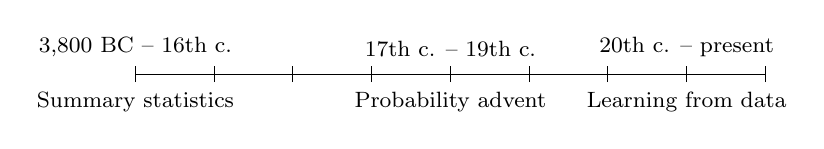
\begin{tikzpicture}
    \draw (0,0) -- (8,0);
    \foreach \x in {0,1,...,8} {
      \draw (\x,-0.1) -- (\x,0.1);
    }
    \foreach \x/\y/\z in {%
        0/Summary statistics/{3,800 BC -- 16th c.},
        4/Probability advent/{17th c. -- 19th c.},
        7/Learning from data/{20th c. -- present}} {
      \node[anchor=north] at (\x,-0.1) {\footnotesize\y};
      \node[anchor=south] at (\x,0.1) {\footnotesize\z};
    }
  \end{tikzpicture}
\end{figurebox}

\Cref{fig:data-analysis-history} illustrates the proposed timeline.  I consider changes of
ages to be smooth transitions, and not strict boundaries.  The theoretical advances are
slower than the technological ones --- the latter influences more data handling than data
analysis ---, so not much has changed since the beginning of the \nth{20} century.

\subsubsection{Summary statistics}

The earliest known records of systematic data analysis date back to the first censuses.
The term \emph{statistics} itself refers to the analysis of data \emph{about the state},
including demographics and economics.  That early (and simplest) form of statistical
analysis is called \emph{summary statistics}, which consists of describing data in terms
of its central tendencies (e.g., arithmetic mean) and variability (e.g., range).

\subsubsection{Probability advent}

However, after the \nth{17} century, the foundations of modern probability theory were
laid out.  Important figures for developing that theory are Blaise Pascal (1623
-- 1662), Pierre de Fermat (1601 -- 1665), Christiaan Huygens (1629 -- 1695), and Jacob
Bernoulli (1655 -- 1705).

The foundation methods brought to life the field of statistical inference. In the
following years, important results were achieved.

\paragraph{Bayes' rule}

Reverend Thomas Bayes (1701 -- 1761) was an English statistician, philosopher, and
Presbyterian minister.  He is known for formulating a specific case of the theorem that
bears his name: Bayes' theorem.  The theorem is used to calculate conditional
probabilities using an algorithm (his Proposition 9, published in 1763) that uses evidence to calculate
limits on an unknown parameter.

The Bayes' rule is the foundation of learning from evidence, once it allows us to
calculate the probability of an event based on prior knowledge of conditions that might be
related to the event.  Classifiers based on Naïve Bayes --- the application of Bayes'
theorem with strong independence assumptions between known variables --- are likely to have
been used since the second half of the eighteenth century.

\paragraph{Gauss' method of least squares}

Johann Carl Friedrich Gauss (1777 -- 1855) was a German mathematician and physicist who made
significant contributions to many fields in mathematics and sciences.  Circa 1794, he
developed the method of least squares for calculating the orbit of Ceres to minimize the
impact of measurement error\footnote{The method was first published by Adrien-Marie
Legendre (1752 -- 1833) in 1805, but Gauss claimed in 1809 that he
had been using it since circa 1794.}.

The method of least squares marked the beginning of the field of regression analysis.  It
marked a shift to find the solution of systems of equations --- especially, overdetermined
systems --- using data instead of theoretical models.

\paragraph{Playfair's data visualization}

Another change in the way we analyze data was the development of data visualization.  Data
visualization is the graphical representation of information and data.

William Playfair (1759 -- 1823) was a secret agent on behalf of Great Britain during its
war with France in the 1790s.  He invented several types of diagrams between the 1780s and
1800s, such as the line, area, and bar chart of economic data, and the pie chart and circle
graph to show proportions.

\subsubsection{Learning from data}

In the twentieth century and beyond, new advances were made in the field of statistics.
The development of learning machines enabled the development of new techniques for data
analysis.

The recent advances in computation and data storage are crucial for the large-scale
application of these techniques.

This era is characterized by a change of focus from trying to fit data to a theoretical
model to trying to extract knowledge from data.  The main goal is to develop algorithms
that can learn from data with minimal human intervention.

\paragraph{Fisher's discriminant analysis}

In the 1930s, Sir Ronald A. Fisher (1890 -- 1962), a British polymath, developed
discriminant analysis\footnote{\url{https://digital.library.adelaide.edu.au/dspace/bitstream/2440/15227/1/138.pdf}},
which was initially used to find linear functions to solve the problem of separating two or
more classes of objects\footnote{After Rosenblatt's work, however, it was used to solve
inductive inference (classification) as well.  For curiosity, Fisher's paper
introduced the famous Iris data set.}.

The method is based on the so-called Fisher discriminant, which is a linear
combination of variables.  The method can be used not only for classification but also for
dimensionality reduction.

Tackling the problem of the importance of the variables for a particular task, Fisher's
work increased the understanding of the importance of feature selection in data analysis.

% See \cref{sub:fisher} for more details about the technique.

\paragraph{Shannon's information theory}

The field --- that studies quantification, storage, and communication of information ---, was
originally established by the works of Harry Nyquist (1889 -- 1976) and Ralph Hartley
(1888 -- 1970) in the 1920s, and Claude Shannon (1916 -- 2001) in the 1940s.
Information theory brought many important concepts to the field of data analysis, such as
entropy, mutual information, and information gain.  This theory is the foundation of
several machine learning algorithms.

Information theory sees data as a sequence of symbols that can be compressed and
transmitted.  The theory is used to quantify the amount of information in a data set.
It also changed dominant paradigms in the field of statistics, such as the use of
likelihood functions and the Bayesian approach.

% See \cref{sub:shannon} for more details about the theory.

\paragraph{K-Nearest Neighbors}

In 1951, Evelyn Fix (1904 -- 1965) and Joseph L. Hodges Jr. (1922 -- 2000) wrote a
technical report entitled ``Discriminatory Analysis, Nonparametric Discrimination:
Consistency Properties.''  In this paper, they proposed the k-nearest neighbors algorithm,
which is a non-parametric method used for classification and regression.  The algorithm
marks a shift from traditional parametric methods --- and purely statistical ones ---
to non-parametric methods.

It also shows how intuitive models can be used to solve complex problems.  The k-nearest
neighbors algorithm is based on the idea that objects that are similar are likely to be in
the same class.

% See \cref{sub:knn} for more details about the technique.

\paragraph{Rosenblatt's perceptron}

In the 1960s, a psychologist called Frank Rosenblatt (1928 -- 1971) developed the perceptron, the first model of
a learning machine.  While the idea of a mathematical neuron was not new, he was the first
to describe the model as a program, showing the ability of the perceptron to learn simple
tasks such as the logical operations AND and OR.

This work was the foundation of the field of artificial neural networks.  The ``training''
of the perceptron was a breakthrough in the field of learning machines, drawing attention
to the field of artificial intelligence.

% In their famous book entitled Perceptrons: An Introduction to Computational Geometry,
% Minsky and Papert show that a perceptron can't solve the XOR problem. This contributed
% to the first AI winter, resulting in funding cuts for neural networks. However, now we
% know that a multilayer perceptron can solve the XOR problem easily.

A few years after, the book ``Perceptrons: an introduction to computational geometry'' by
Marvin Minsky and Seymour Papert in 1969 drew attention to the limitations of the
perceptron\footnote{Although Rosenblatt was aware of the limitations of the perceptron
and was probably working on solutions, he died in 1971.}. They showed that a single-layer
perceptron was limited to linearly separable problems, a fact that led to a decline in the
interest in neural networks.
Consult \cref{sub:perceptron} for more details about the technique.

This fact contributed to the first AI winter, resulting in funding cuts for neural
network research.

\paragraph{Hunt inducing trees}

In 1966, \citeauthor{Hunt1966}'s book\footfullcite{Hunt1966} described a way to induce decision trees from
data.  The algorithm is based on the concept of information entropy and is a precursor of
the \citeauthor{Quinlan1986}'s ID3 algorithm\footfullcite{Quinlan1986} and its variations.
These algorithms gave rise to the field of decision trees, which is a popular method for
classification and regression.

Trees are intuitive models that can be easily interpreted by humans.  They are based on
symbolic rules that can be used to explain their internal decision-making process.

% See \cref{sub:tree} for more details about the technique.

\paragraph{Empirical risk minimization principle}

Although many learning machines were developed until the 1960s, they did not advance
significantly the understanding of the general problem of learning from data.  Between
the 1960s and 1986 --- before the backpropagation algorithm was proposed ---, the field of practical
data analysis was basically stagnant.  The main reason for that was the lack of a
theoretical framework to support the development of new learning machines.

However, these years were not completely unfruitful.  As early as 1968, Vladimir Vapnik
(born 1936)
and Alexey Chervonenkis (1938 -- 2014) developed the fundamental concepts of VC entropy
and VC dimension for data classification problems.  As a result, a novel inductive
principle was proposed: the \gls{erm} principle.
This principle is the foundation of statistical learning theory.

% \paragraph{Algorithmic complexity}
%
% Solomonoff, Kolmogorov, and Chaitin proposed the first learning model based on
% algorithmic complexity.

\paragraph{Resurgence of neural networks}

In 1986, researchers developed independently a method to optimize coefficients of a
multi-layer neural
network\footfullcite{LeCun1986,Rumelhart1986}.  The method is called backpropagation and
is the foundation of the resurgence of neural networks.  The technique enabled the
training of artificial networks that can solve nonlinearly separable problems.

This rebirth of neural networks happened in a scenario very different from the 1960s.
The availability of data and computational power fueled a new approach to the problem of
learning from data.  The new approach preferred the use of simple algorithms and
intuitive models over theoretical models, fueling areas such as bio-inspired computing and
evolutionary computation.

\paragraph{Ensembles}

Following the new approach, ensemble methods were developed.  Based on ideas of
boosting\footfullcite{Schapire1990} and bagging\footfullcite{Breiman1996}, ensemble
methods combine multiple learning machines to improve the performance of the individual
machines.

The difference between boosting and bagging is the way the ensemble is built.  In
boosting, the ensemble is built sequentially, where each new model tries to correct the
errors of the previous models.  In bagging, the ensemble is built in parallel, where each
model is trained independently with small changes in the data.  The most famous bagging
ensemble methods are random forests\footfullcite{Ho1995}, while XGBoost, a gradient
boosting method\footfullcite{Friedman2001}, has been extensively used in machine learning
competitions.

\paragraph{Support vector machines}

In 1995, \textcite{Cortes1995}\footfullcite{Cortes1995} proposed the \gls{svm} algorithm, a
learning machine based on the VC theory and the \gls{erm} principle.  Based on Cover's
theorem\footfullcite{Cover1965}, they developed a method that finds the optimal hyperplane
that separates two classes of data in a high-dimensional space with the maximum margins.
The resulting method led to practical and efficient learning machines.

\paragraph{Deep learning}

Although the idea of neural networks with multiple layers was around since the 1960s,
only in the late 2000s did the field of deep learning catch the attention of the scientific
community by achieving state-of-the-art results in computer vision and natural language
processing.  Yoshua Bengio, Geoffrey
Hinton and Yann LeCun are recognized for their conceptual and engineering
breakthroughs in the field, winning the 2018 Turing Award\footnote{\url{https://awards.acm.org/about/2018-turing}}.

% \paragraph{Knowledge discovery in databases}
%
% In the 1990s, Fayyad, Piatesky-Shapiro, and Smyth
% developed the KDD process, which is the foundation of data mining.
% Data mining is the process of discovering patterns in large data sets involving methods at
% the intersection of machine learning, statistics, and database systems.

% \paragraph{Generative deep models}
%
% Nowadays, generative deep models are a hot topic in machine learning. They are a class of
% statistical models that can generate new data instances. They are used in unsupervised
% learning to discover hidden structures in unlabeled data (e.g., clustering), and in
% supervised learning to generate new synthetic data instances.  The most famous generative
% models are the generative transformers and generative adversarial networks.

\paragraph{LUSI learning theory}

In the 2010s, the researchers \textcite{Vapnik2015}\footfullcite{Vapnik2015} proposed the \gls{lusi}
principle, which is an extension of statistical learning theory.  The \gls{lusi}
theory is based on the concept of statistical invariants, which are properties of
the data that are preserved under transformations.  The theory is the foundation of the
learning from intelligent teachers paradigm.  They regard the \gls{lusi} theory as the
next step in the evolution of learning theory, calling it the ``complete statistical
theory of learning.''

\paragraph{Large Language Models and Attention Mechanisms}

In 2017, \citeauthor{Vaswani2017}\footfullcite{Vaswani2017} proposed the
\emph{transformer} model, a deep learning architecture based on attention mechanisms, in
contrast to recurrent or convolutional neural networks. These architectural
advances --- despite limited theoretical progress --- enabled the development of \glspl{llm},
which gained significant public attention when made widely available by OpenAI in 2020.
That year, OpenAI released a free preview of ChatGPT, a new chatbot capable of generating
human-like text using the \emph{transformer} architecture.

Although generative in nature --- and actually trained as autoregressive models ---
\glspl{llm} proved capable of performing a wide range of tasks, including classification
and reasoning\footnote{Although with some questioning about whether they are actually
reasoning or it is just a mirage: \fullcite{Zhao2025}.}, without the need for
task-specific training.

% vim: set spell spelllang=en:

\chapter{Fundamental concepts}
\label{chap:fundamental}
\glsresetall

\chapterprecishere{The simple believes everything,
  \par\raggedleft but the prudent gives thought to his steps.
  \par\raggedleft--- \textup{Proverbs 14:15} (ESV)}

A useful starting point for someone studying data science is a definition of the term itself.
In this chapter, I discuss some common definitions and provide a definition of my
own.  As discussed in \cref{chap:history}, there is no consensus on the definition of data
science.  However, they all agree that data science is cross-disciplinary and a very
important field of study.

Another important discussion is the evidence that data science is actually a new science.
I argue that a ``new science'' is not a subject whose basis is built from the ground
up\footnote{As it would be as unproductive as creating a ``new math'' for each new
application.  All ``sciences'' rely on each other in some way}, but a subject that has a
particular object of study and that meets some criteria.

Once we establish that data science is a new science, we need to understand one core
concept: data.  In this book, I focus on structured data, which are data that are organized
in a tabular format.  I discuss the importance of understanding the nature of the data we
are working with and how we represent them.

Finally, I discuss two important concepts in data science: database normalization and tidy
data.  Database normalization is mainly focused on data storage.  Tidy data is mainly
focused on the requirements of data for analysis.  Both concepts interact with each other
and have their mathematical foundations.  I bridge the gap between the two concepts by
discussing their common mathematical foundations.

\begin{mainbox}{Chapter remarks}

  \boxsubtitle{Contents}

  \startcontents[chapters]
  \printcontents[chapters]{}{1}{}
  \vspace{1em}

  \boxsubtitle{Context}

  \begin{itemize}
    \itemsep0em
    \item There is no consensus on the definition of data science.
    \item Understanding the nature of data is important to extract knowledge from it.
    \item Structured data are data that are organized in a tabular format.
  \end{itemize}

  \boxsubtitle{Objectives}

  \begin{itemize}
    \itemsep0em
    \item Define data science.
    \item Present the main concepts about data theory.
  \end{itemize}

  \boxsubtitle{Takeaways}

  \begin{itemize}
    \itemsep0em
    \item Data science is a new science that studies the knowledge extraction from
      measurable phenomena using computational methods.
    \item Database normalization and tidy data are complementary concepts that interact
      with each other.
  \end{itemize}
\end{mainbox}

{}
\clearpage

\section{Data science definition}

In literature, we can find many definitions and descriptions of data science.

For \textcite{Zumel2019}\footfullcite{Zumel2019}, \emph{``data science is a cross-disciplinary practice that draws
on methods from data engineering, descriptive statistics, data mining, machine learning,
and predictive analytics.''}  They compare the area with operations research, stating
that data science focuses on implementing data-driven decisions and managing
consequences of these decisions.

\textcite{Wickham2023}\footfullcite{Wickham2023} declare that \emph{``data science is an exciting discipline that
allows you to transform raw data into understanding, insight, and knowledge.''}

\textcite{Hayashi1998}\footfullcite{Hayashi1998} says that data science ``is not only a
synthetic concept to unify statistics, data analysis, and their related methods, but also
comprises its results'' and that it ``intends to analyze and understand actual phenomena
with `data.'{}''

I find the first definition too restrictive once new methods and techniques are always
under development.  We never know when new ``data-related'' methods will become obsolete
or a trend.  Also, \citeauthor{Zumel2019}'s view gives the impression that data science is an
operations research subfield.  Although I do not try to prove otherwise, I think it
is much more useful to see it as an independent field of study.  Obviously, there are
many intersections between both areas (and many other areas as well).  Because of such
intersections, I try my best to keep definitions and
terms standardized throughout chapters, sometimes avoiding popular terms that may generate
ambiguities or confusion.

The second one is not really a definition.  However, it states clearly \emph{what} data
science enables us to do.  The terms ``understanding,'' ``insight,'' and ``knowledge'' are
very important in the context of data science.  They are the goals of a data science
project.

The third definition brings an important aspect behind the data: the phenomena from which
they come.  Data science is not only about data, but about understanding the phenomena
they represent.

Note that these definitions do not contradict each other.  But, they do not attempt to
emphasize the ``science'' aspect of it.  From these ideas, let us define the term.

\begin{defbox}{Data science}{ds}
  Data science is the study of knowledge extraction from
  measurable phenomena using computational methods.
\end{defbox}

I want to highlight the meaning of some terms in this definition.  \emph{Computational methods} means
that data science methods use computers to handle data and perform the calculations.
\emph{Knowledge} means information that humans can understand and/or apply to solve
problems.  \emph{Measurable phenomena} are events or processes where raw data can be
quantified in some way\footnote{%
  Non-measurable phenomena are related to metaphysics and are not the object of study in
  data science.  They are the object of study in other sciences, such as
  philosophy, theology, etc.  However, many concepts from metaphysics are borrowed to
  explain data science concepts.%
}.  \emph{Raw data} are data collected directly from some source and
that have not been subject to any transformation by a software program or a human
expert.  \emph{Data} is any piece of information that can be digitally stored.


\textcite{Kelleher2018}\footfullcite{Kelleher2018} summarize very well the challenges of data science:
``extracting non-obvious and useful patterns from large data sets [\dots]; capturing,
cleaning, and transforming [\dots] data; [storing and processing] big [\dots] data sets;
and questions related to data ethics and regulation.''

Data science naming contrasts with conventional sciences.  Usually, a ``science'' is named after
its object of study.  Biology is the study of life, Earth science studies the planet
Earth, and so on.  I argue that data science does not study data itself, but how we can
use it to understand a certain phenomenon.

One similar example is ``computer science.''  Computer science is not the study of
computers themselves, but the study of computing and computer systems.  Similarly, one
could state that data science studies knowledge extraction\footnote{Related to data
analysis, see \cref{sub:time-analysis}.} and data systems\footnote{Related to data
handling, see \cref{sub:time-handling}.}.

Moreover, the conventional scientific paradigm is
essentially model-driven: we observe a phenomenon related to the object of study, we
reason about the possible explanation (the model or hypothesis), and we validate our hypothesis
(most of the time using data, though).  In data science, however, we extract knowledge
directly and primarily from the data.  Expert knowledge and reasoning may be taken
into account, but we give data the opportunity to surprise us.

Thus, while the objects of study in conventional sciences are the phenomena themselves
and the models that can explain them, the objects of study in data
science are the means (computational methods and processes) that can extract reliable and ethical
knowledge from data acquired from any measurable phenomenon --- and, of course, their
consequences.

\def\verrids{(0,0) circle (20mm)}
\def\verrist{(-2.5,0) circle (15mm)}
\def\verride {(2.5,0) circle (15mm)}
\def\verrics {(0,-2.5) circle (15mm)}

\begin{figurebox}[label=fig:myview]{My view of data science.}
  \centering
  \begin{tikzpicture}
    \begin{scope}
      \clip \verrids;
      \fill[filled] \verrist;
      \fill[filled] \verride;
      \fill[filled] \verrics;
    \end{scope}
    \draw[outline] \verrids node(ds) {};
    \draw[outline] \verrist node {Statistics};
    \draw[outline, text width=27mm, text centered] \verride node {Philosophy / domain expertise};
    \draw[outline] \verrics node {Computer science};
    \node[anchor=north,above] at (0, 1) {Data science};
  \end{tikzpicture}
  \tcblower
    Data science is an entirely new science.  Being a new science
    does not mean that its basis is built from the ground up.  Most of the subjects in
    data science come from other sciences, but its object of study (computational methods
    to extract knowledge from measurable phenomena) is particular enough to unfold
    new scientific questions -- such as data ethics, data collection, etc.
    Note that I emphasize philosophy over domain expertise because, in terms
    of scientific knowledge, the former is more general than the latter.
\end{figurebox}

\Cref{fig:myview} shows my view of data science.  Data science is an entirely new science
that incorporates concepts from other sciences.  In the next section, I argue the reasons
to understand data science as a new science.

\section{The data science continuum}

In the previous section, I argued that data science is a new science defining its object
of study.  This is just the first step to establish a new science, especially because the
object of study in data science is not new.  Computer science, statistics, and other
sciences have been studying methods to process data for a long time.

One key aspect of the establishment of a new science is the social demand and the
importance of the object of study in our society.  Many say that ``data is the new oil.''
This is because the generation, storage, and processing of data has increased exponentially
in the last decades.  As a consequence, whoever holds the data and can effectively extract
knowledge from them has a competitive advantage.

As a consequence of the demand, a set of methods are developed and then experiments are
designed to assess their effectiveness.  If the methods are effective, they gain
credibility, are widely accepted, and become the foundation of a new scientific
discipline.

Usually, a practical consequence of academic recognition is the creation of new courses
and programs in universities.  This is the case of data science.  Many universities have
created data science programs in the last few years.

Once efforts to develop the subject increase, it is natural that some methodologies and
questions not particularly related to any other science evolve.  This effect produces what I
call the ``data science continuum.''

In a continuum, the subject is not a new science yet.  It is a set of methods and
techniques borrowed from other sciences.  However, some principles emerge that are
connected with more than one already established science.  (For instance, a traditional
computational method adapted to assume statistical properties of the data.)  With time,
the premises and hypotheses of new methods become distinctive.  The particular properties
of the methods lead to the inception of methodologies to validate them. While validating
the methods, new questions arise.

\begin{figurebox}[label=fig:continuum]{The data science continuum.}
  \centering
  \begin{tikzpicture}[node distance=10mm and 3mm]
    % Base Layer: Established Sciences
    \node (stats) [block] {Statistics};
    \node (cs) [block, right=of stats] {Computer science};
    \node (ds) [block, right=of cs] {Philosophy and others};
    % A box around the Base Layer
    \node (basebox) [draw, dashed, inner sep=0.5cm, fit={(stats) (ds)}, label=above:{Established sciences}] {};
    % Middle Layer: Emergence of Principles
    \node (principles) [darkblock, below=of basebox, minimum width=6cm, text width=5cm] {Emergence of principles};
    % Top Layer: Unique Methods and Validation
    \node (methods) [block, below=of principles, minimum width=6cm, text width=5cm] {Unique methods};
    \node (validation) [darkblock, below=of methods, minimum width=6cm, text width=5cm] {Validation and new challenges};
    \node (science) [block, below=of validation, minimum width=6cm, text width=5cm] {Data science};
    % Arrows
    \draw[-{Stealth}] (basebox) -- (principles);
    \draw[-{Stealth}] (principles) -- (methods);
    \draw[-{Stealth}] (methods) -- (validation);
    \draw[-{Stealth}] (validation) -- (science);
  \end{tikzpicture}
  \tcblower
    The data science continuum is the process of development of data science as a new
    science.  It began by borrowing methods and techniques from established sciences. Over
    time, distinct principles emerged that spanned multiple disciplines. As these
    principles developed, new methods and their premises became unique. This uniqueness
    led to the creation of specific methodologies for validating these methods. During the
    validation process, new questions and challenges arose, further distinguishing data
    science from its parent disciplines.
\end{figurebox}

The data science continuum is an instance of this process; see \cref{fig:continuum}.  At
first glance, data science seems like just a combination of computer science, statistics,
linear algebra, etc. However, the principles and priorities of data science are not the
same as those in these disciplines. Similarly, the accepted methodologies in data science
differ and keep evolving from those in other sciences. New questions arise, such as:
\begin{itemize}
  \itemsep0em
  \item How can we guarantee that the data we are using is reliable?
  \item How can we collect data in a way that does not bias our conclusions?
  \item How can we guarantee that the data we are using is ethical?
  \item How can we present our results in a way that is understandable to non-experts?
\end{itemize}

\section{Fundamental data theory}

As I stated, data science is not an isolated science. It incorporates several concepts
from other fields and sciences.  In this section, I explain the basis of each component of
\cref{def:ds}.

\subsection{Phenomena}
\label{sub:phenomena}

Phenomenon is a term used to describe any observable event or process.  They are the
source we use to understand the world around us.  In general, we use our senses to
perceive phenomena.  To make sense of them, we use our knowledge and reasoning.

Philosophy is the study of knowledge and reasoning.  It is a very broad field of study
that has been divided into many subfields.  One possible starting point is \gls{ontology},
which is the study of being, existence, and reality.  Ontology studies what exists and how
we can classify it.  In particular, ontology describes the nature of categories,
properties, and relations.

Aristotle (384 -- 322 BC) is one of the first philosophers to study ontology. In
Κατηγορίαι\footnote{For Portuguese readers, I suggest \fullcite{CategoriesUnesp}.}, he
proposed a classification of the world into ten categories. Substance, or οὐσία,
is the most important one.  It is the category of being.  The other categories
are properties, quantity, quality, relation, place, time, position, state, and action.

Although rudimentary\footnote{Most historians agree that Categories was written before
Aristotle's other works.  Many concepts are further developed in his later works.},
Aristotle's categories served as a basis for the development of logical reasoning and
scientific classification, especially in the Western world.  The categories are still
used in many applications, including computer systems and data systems.

Aristotle marked a rupture with many previous philosophers.  While Heraclitus (\nth{6}
century -- \nth{5} century BC) defended that everything is in a constant state of flux and
Plato (c. 427 -- 348 BC) defended that only the perfect can be known, Aristotle focused on
the world we can perceive and understand.  His practical view also opposed Antisthenes (c.
446 -- 366 BC) view that the predicate determines the object, which leads to the
impossibility of negation and consequently contradiction.

What is the importance of ontology for data science?  Describing, which is basically
reducing the complexity of the world to simple, small pieces, is the first step to
understand any phenomenon.  Drawing a simplistic parallel, phenomena are like the
substance category, and the data we collect are like the other categories, which describe
the properties, relations, and states of the substance.  A person who can easily organize
their thoughts to identify the entities and their properties in a problem is more likely
to collect relevant data.  Also, the understanding of logical and grammatical limitations
--- such as univocal and equivocal terms --- is important to avoid errors in data
science applications\footnote{It is very common to see data scientists reducing the
meaning of the columns in a dataset to a single word.  Or even worse, they assume
that different columns with the same name have the same meaning.  This is a common source
of errors in data science projects.}.

Another important field in Philosophy is epistemology, which is the study of knowledge.
Epistemology elaborates on how we can acquire knowledge and how we can distinguish between
knowledge and opinion.  In particular, epistemology studies the nature of knowledge,
justification, and the rationality of belief.

Finally, logic is the study of reasoning.  It studies the nature of reasoning and
argumentation.  In particular, logic studies the nature of inference, validity, and
fallacies.

I further discuss knowledge and reasoning in \cref{sub:knowledge}.

In the context of a data science project, we usually focus on phenomena from a particular domain of
expertise.  For example, we may be interested in phenomena related to the stock
market, or related to the weather, or related to human
health.  Thus, we need to understand the nature of the phenomena we are studying.

Fully understanding the phenomena we are tackling requires both general knowledge
of epistemology, ontology, and logic, and particular knowledge of the domain of
expertise.

Observe as well that we do not restrict ourselves to the intellectual understanding of
philosophy.  There are several computational methods that implement the concepts of
epistemology, ontology, and logic.  For example, we can use a computer to perform
deductive reasoning, to classify objects, or to validate an argument.  Also, we have
strong mathematical foundations and computational tools to organize categories, relations, and
properties.

The reason we need to understand the nature of the phenomena we are studying is that we
need to guarantee that the data we are collecting are relevant to the problem we are
trying to solve.  An incorrect perception of the phenomena may lead to incorrect data
collection, which certainly leads to incorrect conclusions.

\subsection{Measurements}

Similarly to Aristotle's work, data scientists focus on the world we can perceive with our
senses (or using external sensors).  In a more restrictive way, we focus on the world we
can measure\footnote{Some phenomena might be knowable but not measurable.  For example,
the existence of God is a knowable phenomenon, but it is not measurable.}. Measurable
phenomena are
those that we can quantify in some way.  For example, the temperature of a room is a
measurable phenomenon because we can measure it using a thermometer.  The number of
people in a room is also a measurable phenomenon because we can count them.

When we quantify a phenomenon, we perform data collection.  Data collection is the process
of gathering data on a targeted phenomenon in an established systematic way.
Systematic means that we have a plan to collect the data and we understand the
consequences of the plan, including the sampling bias.  Sampling bias is the influence
that the method of collecting the data has on the conclusions we can draw from them.
Once we have collected the data, we need to store them.  Data storage is the process of
storing data in a computer.

To perform those tasks, we need to understand the nature of data.  Data are any piece of
information that can be digitally stored.  Data can be stored in many different formats.
For example, we can store data in a spreadsheet, in a database, or in a text file.  We can
also store data in many different types.  For example, we can store data as numbers,
strings, or dates.

In data science, studying data types is important because they need to correctly reflect
the nature of the source phenomenon and be compatible with the computational methods we
are using.  Data types also restrict the operations we can perform on the data.

The foundation and tools to understand data types come from computer science.  Among the
subfields, I highlight:
\begin{itemize}
  \itemsep0em
  \item Algorithms and data structures: the study of data types and the computational
    methods to manipulate them.
  \item Databases: the study of storing and retrieving data.
\end{itemize}

The fundamental concepts are the same independently of the programming language, hardware
architecture, or the \gls{rdbms} we are using.  As a consequence, in this book, I focus on
the concepts and not on the tools.

\subsection{Knowledge extraction}
\label{sub:knowledge}

Like discussed before, knowledge and reasoning are important aspects of data science.
Philosophical and mathematical foundations from epistemology and logic provide us with ways
to obtain knowledge from a set of premises and known (and accepted) facts\footnote{In
mathematics, axioms are the premises and accepted facts.  Corollaries,
lemmas, and theorems are the results of the reasoning process.}.

Deductive reasoning is the process of deriving a conclusion (or new knowledge) from
a set of previous knowledge.  Deductive reasoning, thus, enables us to infer
generalization rules from known general rules.

Important figures that bridged the gap between the subjects of philosophy and mathematics are
René Descartes (1596 -- 1650) and Gottfried Wilhelm Leibniz (1646 -- 1716).  Descartes
was the first to use algebra to solve knowledge problems, effectively creating
methods to mechanize reasoning.  Leibniz, after Descartes, envisioned a universal
algebraic language that would encompass logical principles and methods. Their work
influenced the development of calculus, Boolean algebra, and many other fields.

Once we have collected and stored the data, the next step is to extract knowledge from them.
Knowledge extraction is the process of obtaining knowledge from data.  The reasoning
principle here is inductive reasoning.  Inductive reasoning is the process of deriving
generalization rules from specific observations.  Inductive reasoning and data analysis
are closely related.  Refer to \cref{sub:time-analysis} for a timeline of the development
of data analysis.

In data science, we use computational methods to extract knowledge from data.  These
computational methods may come from many different fields.  In particular, I highlight:
\begin{itemize}
  \itemsep0em
  \item Statistics: the study of data collection, organization, analysis, interpretation,
    and presentation.
  \item Machine learning: the study of computational methods that can automatically learn from data.
    It is a branch of artificial intelligence.
  \item Operations research: the study of computational methods to optimize decisions.
\end{itemize}

Also, many other fields contribute to the development of domain-specific computational
methods to extract knowledge from data.  For example, in the field of biology, we have
bioinformatics, which is the study of computational methods to analyze biological data.
Earth sciences have geoinformatics, which is the study of computational methods to
analyze geographical data.  And so on.

Each method has its own assumptions and limitations.  Thus, we need to understand the
nature of the methods we are using.  In particular, we need to understand the
expected input and output of them.  Whenever the available data do not match the
requirements of the technique, we may perform data preprocessing\footnote{%
  It is important to highlight that it is expected that some of the method's assumptions
  are not fully met.  These methods are usually robust enough to extract valuable
  knowledge even when data contain imperfections, errors, and noise.  However, it is still
  useful to perform data preprocessing to adjust data as much as possible.%
}.

Data preprocessing mainly includes data cleaning, data transformation, and data
enhancement. Data cleaning is the process of detecting and correcting (or removing)
corrupt or inaccurate pieces of data.  Data transformation is the process of converting
data from one format or type to another.  Data enhancement is the process of adding
additional information to the data, usually by integrating
data from different sources into a single, unified view.

% vim: set spell spelllang=en:

\chapter{Data science project}
\label{chap:project}
\glsresetall

% TODO(v0.2): talk about documentation and more about deployment in the future

\chapterprecishere{\raggedleft\textup{with contributions from} \textsc{Johnny C. Marques}~\orcidlink{0000-0002-1551-435X}
  \\[5mm] Figured I could throw myself a pity party or go back to school and learn the computers.
  \par\raggedleft--- \textup{Don Carlton}, Monsters University (2013)}

Once we have established what data science is, we can now discuss how to conduct a data science
project.
First of all, \emph{a data science project is a software project}.  The difference between a data
science software and a traditional software is that some components of the former are
constructed from data.  This means that part of the solution is not designed from the
knowledge of the domain expert.

One example of a project is a spam filter that
classifies emails into two categories: spam and non-spam.  A traditional approach is
to design a set of rules that are known to be effective.  However, the effectiveness of
the filters is limited by the knowledge of the designer and is cumbersome to maintain.  A
data science approach automatically learns the filters from a set of
emails that are already classified as spam or non-spam.

Another important difference in data science projects is that traditional testing methods,
such as unit tests, are not sufficient. The solution inferred from the data must be validated
considering the stochastic nature of the data.

In this chapter, we discuss common methodologies for data science projects.  We also
present the concept of agile methodologies and the Scrum framework.  We finally propose an
extension to Scrum adapted for data science projects.

\begin{mainbox}{Chapter remarks}

  \boxsubtitle{Contents}

  \startcontents[chapters]
  \printcontents[chapters]{}{1}{}
  \vspace{1em}

  \boxsubtitle{Context}

  \begin{itemize}
    \itemsep0em
    \item A data science project is a software project.
    \item Data science methodologies focus on the data analysis process.
    \item The industry demands not only data analysis but also software development.
  \end{itemize}

  \boxsubtitle{Objectives}

  \begin{itemize}
    \itemsep0em
    \item Explore common methodologies for data science projects.
    \item Understand agile methodologies and the Scrum framework.
    \item Propose an extension to Scrum adapted for data science projects.
  \end{itemize}

  \boxsubtitle{Takeaways}

  \begin{itemize}
    \itemsep0em
    \item Modern data science methodologies take into account the software development aspects of the
      project.
    \item Scrum is a good framework for software development, and it can be adapted for
      data science projects.
  \end{itemize}
\end{mainbox}

{}
\clearpage

\section{CRISP-DM}

CRISP-DM\footnote{Official guide available at
\url{https://www.ibm.com/docs/it/SS3RA7_18.3.0/pdf/ModelerCRISPDM.pdf}.} is a methodology
for data mining projects.  It is an acronym for Cross Industry Standard Process for Data
Mining.  It is a methodology that was developed in the 1990s by IBM, and it is still
widely used today.

CRISP-DM is a cyclic process.  The process is composed of six phases:
\begin{enumerate}
  \item Business understanding: this is the phase where the project objectives are
    defined.  The objectives must be defined in a way that is measurable.  The phase also
    includes the definition of the project plan.
  \item Data understanding: this is the phase where the data is collected and explored.
    The data is collected from the data sources, and it is explored to understand its
    characteristics.  The phase also includes the definition of the data quality
    requirements.
  \item Data preparation: this is the phase where the data is prepared for the modeling
    phase.  The data is cleaned, transformed, and aggregated.  The phase also includes the
    definition of the modeling requirements.
  \item Modeling: this is the phase where the model is trained and validated.  The model is
    trained using the prepared data, and it is validated using the validation data.  The
    phase also includes the definition of the evaluation requirements.
  \item Evaluation: this is the phase where the model is evaluated.  The model is evaluated
    using the evaluation data.  The phase also includes the definition of the deployment
    requirements.
  \item Deployment: this is the phase where the model is deployed.  The model is deployed
    using the deployment requirements.  The phase also includes the definition of the
    monitoring requirements.
\end{enumerate}

CRISP-DM is cyclic and completely focused on the data.  However, it does not address the
software development aspects of the project.  The ``product'' of the project is both
models and findings, not the full software solution.  As a result, aspects such as user
interface, communication, and integration are not addressed by the methodology.

\clearpage

\begin{figurebox}[label=fig:cripdm]{Diagram of the CRISP-DM process.}
  \centering
  \begin{tikzpicture}
    \node (1) at (0, 0) {};
    \node (2) at (4, -4) {};
    \node (3) at (0, -8) {};
    \node (4) at (-4, -4) {};

    \node [block] (bu) at (-1.5, -2) {Business understanding};
    \node [block] (du) at (1.5, -2) {Data understanding};
    \path [line] (bu) -- (du);
    \path [line] (du) -- (bu);

    \node [block] (dp) at (2.5, -3.5) {Data preparation};
    \node [block] (m) at (2.5, -5) {Modeling};
    \path [line] (dp) -- (m);
    \path [line] (m) -- (dp);

    \path [line] (du) -- (dp);

    \node [block] (e) at (0, -6.5) {Evaluation};
    \node [block] (d) at (-2.5, -4.25) {Deployment};

    \path [line] (m) -- (e);
    \path [line] (e) -- (d);
    \path [line] (e) -- (bu);

    \node [draw, circle, fill=gray, text centered, text=white] at (0, -4.25) {Data};

    \path [bigarrow] (1.east) to[out=0, in=90] (2.60);
    \path [bigarrow] (2.-60) to[out=-90, in=0] (3.east);
    \path [bigarrow] (3.west) to[out=180, in=-90] (4.-120);
    \path [bigarrow] (4.120) to[out=90, in=180] (1.west);
  \end{tikzpicture}
  \tcblower
  Each block represents a phase of the CRISP-DM process.  Data is the central element of
  the process.  Arrows represent the transitions between the phases.
\end{figurebox}

\Cref{fig:cripdm} shows a diagram of the CRISP-DM process.  The double arrow between the
business understanding and the data understanding phases represents the iterative nature
of these steps.  Once we are satisfied with the data understanding, we can proceed to
the data preparation phase.  The same iteration is possible between the data preparation
and the modeling phases, since modeling methods can require different data preparation
methods. Finally, an evaluation is performed.  If the model is satisfactory, we proceed to the
deployment phase.  Otherwise, we return to the business understanding phase.  The idea
is to revisit the project objectives and, if necessary, the project plan.

The CRISP-DM methodology is a good starting point for data science projects.  However, it
does not mean that it should be followed strictly.  The process is flexible, and
adaptations are possible at any stage.

\section{ZM approach}

\textcite{Zumel2019}\footfullcite{Zumel2019} also propose a methodology for data science projects --- which we
call here the ZM approach.  Besides
describing each step in a data science project, they further address the roles of each
individual involved in the project.  They state that data science projects are always
collaborative, as they require domain expertise, data expertise, and software expertise.

Requirements of a data science project are dynamic, and we need to perform many
exploratory phases.  Unlike traditional software projects, we should expect significant
changes in the initial requirements and goals of the project.

Usually,
projects based on data are urgent, and they must be completed in a short time --- not
only due to the business requirements, but also because the data changes over time.
The authors state that agile methodologies are suitable (and necessary) for data science
projects.

\subsection{Roles of the ZM approach}

In their approach, they define five roles.  The roles are:

\paragraph{Project sponsor}  It is the main stakeholder of the project, the one that needs the
results of the project.  He represents the business interests and champions the project.
The project is considered successful if the sponsor is satisfied.  Note that, ideally, the
sponsor cannot be the data scientist, but someone who is not involved in the development
of the project.  However, he needs to be able to express \emph{quantitatively} the business
goals and participate actively in the project.

\paragraph{Client}  The client is the domain expert.  He represents the end users'
interests.  In a small project, he is usually the sponsor.  He translates the daily
activities of the business into the technical requirements of the software.

\paragraph{Data scientist}  The data scientist is the one that sets and executes the
analytic strategy.  He is the one that communicates with the sponsor and the client,
effectively connecting all the roles.  In small projects, he can also act as the developer
of the software.  However, in large projects, he is usually the project manager.
Although it is not required to be a domain expert, the data scientist must be able to
understand the domain of the problem.  He must be able to understand the business goals and
the client's requirements.  Most importantly, he must be able to define and solve the
right tasks.

\paragraph{Data architect}  The data architect is the one that manages data and data storage.
He usually is involved in more than one project, so he is not an active participant.  He
is the one who receives instructions to adapt the data storage and means to collect data.

\paragraph{Operations}  The operations role is the one that manages infrastructure and
deploys final project results.  He is responsible for defining requirements such as response
time, programming language, and the infrastructure to run the software.

\subsection{Processes of the ZM approach}

\citeauthor{Zumel2019}'s model is similar to CRISP-DM, but emphasizes that back-and-forth
is possible at any stage of the process.  \Cref{fig:zumel} shows a diagram of the process.
The phases and the answers we are looking for in each phase are:
\begin{itemize}
  \itemsep0em
  \item Define the goal: what problem are we trying to solve?
  \item Collect and manage data: what information do we need?
  \item Build the model: what patterns in the data may solve the problem?
  \item Evaluate the model: is the model good enough to solve the problem?
  \item Present results and document: how did we solve the problem?
  \item Deploy the model: how to use the solution?
\end{itemize}

The step ``Present results and document'' is a differentiator from the other approaches, like
CRISP-DM.  In the ZM approach, result presentation is essential; data scientists must be able
to communicate their results effectively to the client/sponsor.  This phase is also
emphasized in the view of \textcite{Wickham2023}.

\begin{figurebox}[label=fig:zumel]{Diagram of the data science process proposed by \textcite{Zumel2019}.}
  \centering
  \begin{tikzpicture}
    \node (1) at (0, 0) {};
    \node (2) at (1, -1) {};
    \node (3) at (0, -2) {};
    \node (4) at (-1, -1) {};
    \path [bigarrow] (1.east) to[out=0, in=90] (2.60);
    \path [bigarrow] (2.-60) to[out=-90, in=0] (3.east);
    \path [bigarrow] (3.west) to[out=180, in=-90] (4.-120);
    \path [bigarrow] (4.120) to[out=90, in=180] (1.west);

    \node [block] (dg) at (0, 1) {Define the goal};
    \node [block] (cm) at (3, -0.25) {Collect and manage data};
    \node [block] (bm) at (3, -1.75) {Build the model};
    \node [block] (em) at (0, -3) {Evaluate the model};
    \node [block] (pd) at (-3, -1.75) {Present results};
    \node [block] (dm) at (-3, -0.25) {Deploy the model};

    \path [dline] (dg) to[out=0, in=90] (cm.north);
    \path [dline] (cm) -- (bm);
    \path [dline] (bm.south) to[out=-90, in=0] (em.east);
    \path [dline] (em.west) to[out=180, in=-90] (pd.south);
    \path [dline] (pd) -- (dm);
    \path [dline] (dm.north) to[in=180, out=90] (dg.west);
  \end{tikzpicture}

  \tcblower
  Each block represents a phase of the data science process.  The emphasis is on the
  cyclic nature of the process.  Arrows represent the transitions between the phases, which
  can be back-and-forth.
\end{figurebox}

\subsection{Limitations of the ZM approach}

The ZM approach is particularly interesting in consulting projects, as the data scientist
is not part of the organization.  Note that tasks beyond deployment, such as maintenance and
monitoring, are not directly addressed by the methodology but are delegated to the operations
role.  Like CRISP-DM, the ZM approach does not address the software development aspects of
the project.

\section{Agile methodology}

Agile is a methodology for software development.  It is an alternative to the waterfall
methodology.  The waterfall methodology is a sequential design where each phase
must be completed before the next phase can begin.

The methodology is based on the four values of the Agile Manifesto\footnote{\url{https://agilemanifesto.org/}}:
\begin{itemize}
  \itemsep0em
  \item Individuals and interactions over processes and tools;
  \item Working software over comprehensive documentation;
  \item Customer collaboration over contract negotiation;
  \item Responding to change over following a plan.
\end{itemize}

Note that the manifesto does not discard the items on the right, but rather values the items on
the left more.  For example, comprehensive documentation is important, but working software
is more important.

\section{Scrum framework}

The Scrum framework is one of the most widely adopted agile methodologies. It is an
iterative, incremental process that enables teams to deliver high-value products
efficiently while adapting to changing requirements. Scrum emphasizes teamwork,
accountability, and continuous improvement. Developed by \textcite{schwaber2020scrum}%
\footnote{Latest version of the Scrum Guide available at \fullcite{schwaber2020scrum}.}
in the early 1990s, Scrum is based on three pillars: transparency, inspection, and
adaptation. These principles help teams to navigate complex, adaptive problems and deliver
productive outcomes.

Scrum organizes work into cycles called sprints, and involves defined roles, ceremonies,
and artifacts that ensure the progress and quality of the product. Key events such as
daily stand-ups, retrospectives, and sprint reviews create regular opportunities to inspect
and adapt, making Scrum a responsive and resilient framework\footfullcite{denning2016scrum}.

\subsection{Scrum roles}

Scrum defines three critical roles: the product owner, the Scrum master, and the
development team.
Each of these roles has specific responsibilities, and together they ensure that the Scrum
process runs smoothly and that the product development aligns with the overall business
objectives.

\paragraph{Product owner} This role is responsible for defining the product vision and
    maximizing the value of the work done by the team. The product owner manages the
    product backlog, ensuring that it is visible, transparent, and prioritized according
    to business needs. They serve as the main point of contact between stakeholders and
    the development team\footfullcite{openagile2019roles}. The product owner must constantly
    balance the requirements of the business and the technical capabilities of the team,
    ensuring that the highest-value items are worked on first.

\paragraph{Scrum master} The Scrum master acts as a facilitator and coach for the Scrum team,
    ensuring that the team adheres to the Scrum framework and agile principles. Unlike a
    traditional project manager, the Scrum master is not responsible for managing the team
    directly but for enabling them to perform optimally by removing impediments and
    fostering a self-organizing culture\footfullcite{cobb2015scrum}.

\paragraph{Development team} It is a cross-functional group of professionals
    responsible for delivering potentially shippable product increments at the end of each
    sprint. The team is self-managing, meaning they decide how to achieve their goals
    within the sprint. The team is small enough to remain nimble but large enough
    to complete meaningful work\footfullcite{rubin2012sprints}. The development team works
    collaboratively and takes collective responsibility for the outcome of the sprint.

\subsection{Sprints and backlog}

A sprint is the basic unit of work in Scrum, as presented in \cref{fig:scrum}. Sprints
are time-boxed iterations, usually lasting between one to four weeks, during which a
defined amount of work is completed. The goal is to deliver a potentially shippable
product increment at the end of each sprint. Sprints are continuous, with no breaks in
between, fostering a regular, predictable rhythm of work\nocite{cobb2015scrum}.

\begin{figurebox}[label=fig:scrum]{Scrum framework overview.}
    \centering
    \begin{tikzpicture}[%
        font=\LARGE,
        every label/.style={font=\footnotesize},
      ]
      \node[align=center, label=below:product owner] (po) at (0.9, 0) {\faUserTie};
      \node[align=center, label=below:product backlog] (backlog) at (0.9, -1.5) {\faListOl};

      \node[align=center, label=below:dev team] (dev) at (3.2, 0) {\faUsers};
      \node[align=center, label=below:sprint backlog] (sbacklog) at (3.2, -1.5) {\faClipboardList};

      \draw[-Stealth] (backlog) -- (sbacklog) node[midway, above, font=\footnotesize, yshift=2mm] {sprint planning};

      \draw[-Stealth, very thick] (sbacklog.east)
        to[out=0, in=180] (5.6, -1.5)
        to[out=0, in=0] (5.6, 0.5)
        to[out=0, in=0] (5, 0.5)
        to[out=180, in=130] (4.7, -1.4);

      \node[font=\footnotesize] at (5.2, -0.5) {sprint};

      \node[align=center, label=above:Scrum master] (sm) at (4.2, 0.8) {\faUser};

      \draw[-Stealth, very thick] (6, -1.5) -- (7, -1.5);

      \draw[-Stealth] (5.7, 0.6)
        to[out=120, in=200] (5.8, 1)
        to[out=20, in=160] (6.2, 1)
        to[out=-20, in=20] (6, 0.3);

      \node[draw, rectangle, dashed, align=center, label=below:daily scrum] (daily) at (7, 2) {\faUser \faUsers};
      \draw[-] (daily.south west) -- (6, 0.8);

      \node[draw, rectangle, dashed, align=center, label=above:sprint review] (review) at (7.8, 0) {\faUser~\faUsers};
      \node[draw, rectangle, dashed, align=center, label=above:incremental version] (version) at (7.8, -1.3) {\faBox~\faUserTie};
      \node[draw, rectangle, dashed, align=center, label=above:sprint retrospective] (retrospective) at (7.8, -2.6) {\faUserTie~\faUser~\faUsers};
    \end{tikzpicture}
    \tcblower
    The development centers around the sprints, which are time-boxed iterations.  Roles,
    other ceremonies, and artifacts support the sprints and ensure the progress and
    quality of the product.
\end{figurebox}

Before a sprint starts, the Scrum team holds a sprint planning meeting to decide what will
be worked on. The work for the sprint is selected from the product backlog, which is a
prioritized list of features, enhancements, bug fixes, and other deliverables necessary
for the product\nocite{schwaber2020scrum}. The product backlog is dynamic and evolves as
new requirements and changes emerge. The items selected for the sprint become part of the
sprint backlog, a subset of the product backlog that the development team commits to
completing during the sprint.

At the heart of the Scrum process is the daily scrum (or stand-up meeting), a brief
meeting where the team discusses progress toward the sprint goal, any obstacles they are
facing, and their plans for the next day. This daily inspection ensures that everyone
stays aligned and can quickly adapt to any changes or challenges\nocite{cobb2015scrum}.

The burn down/up chart is a visual tool used during the sprint to track the Scrum
team's progress against the planned tasks. It displays the amount of remaining work (in
hours or story points) over time, allowing the team and the product owner to monitor
whether the work is on pace to be completed by the end of the sprint. The chart's line
decreases as tasks are finished, providing a clear indicator of potential delays or
blockers. If progress is falling behind, the team adjusts the approach during the
sprint by re-prioritizing tasks or removing impediments. Thus, this chart provides
real-time visibility into the team’s efficiency and contributes to more agile and
proactive work management.

At the end of each sprint, the team holds a sprint review, where they demonstrate the work
completed and gather feedback from stakeholders. This feedback may lead to adjustments in
the Product Backlog and ensures that progress remains aligned with expectations.
Immediately after, the team conducts a sprint retrospective, a crucial Scrum event focused
on reflecting on the sprint that just concluded. In the retrospective, they discuss what
went well, what challenges they encountered, and how they can enhance their workflow and
collaboration. These continuous cycles of review and reflection not only drive incremental
improvement but also foster transparency, team cohesion, and sustained productivity.
\nocite{rubin2012sprints}

\subsection{Scrum for data science projects}

Some consider that Scrum is not adequate for data science projects.  The main reason is
that Scrum is designed for projects where the requirements are known in advance.  Also,
data-driven exploratory phases are not well supported by Scrum.

I argue that this view is wrong.  Scrum is a framework, and it is designed to be adapted to
the needs of the project;  Scrum is not a rigid process.  In the following, I propose an
extension to Scrum that makes it suitable for data science projects\footnote{Note that
many other adaptations to Scrum have been described in literature.  For example,
\fullcite{Saltz2019,Baijens2020,Kraut2022}.}.

One of my major concerns in the proposal of the extension is that data science projects
usually involve ``data scientists'' who are not primarily developers, but statisticians or
domain experts.  They usually do not possess ``hacking-level'' skills, and they often do not know
good practices of software development.

Scrum is a good starting point for a compromise between the need for autonomy (required in
dynamic and exploratory projects) and the need for a detailed plan to guide the project
(required to avoid bad practices and low-quality software). A good project methodology is
needed to ensure that the project is completed on time and within budget.

\section{Our approach}
\label{sec:our-approach}
% TODO: talk about nowadays clients expect the final product, not only the model
% TODO: talk about unrealistic separation between preparation, modeling and evaluation,
% specially when considering machine learning

The previously mentioned methodologies lack focus on the software development aspects of
the data science project.  For instance, CRISP-DM defines the stages only of the data
mining process, i.e., it does not explicitly address user interface or data collection.
\citeauthor{Zumel2019}'s approach addresses data collection and presentation of results, but
delegates software development\footnote{Although, they do address it in a prototyping level, but
not in a production level.} to the operations role, barely mentioning it.  Scrum is
a good framework for software development, but it is not designed for data science
projects.  For instance, it lacks the exploratory phases of data science projects.

For the sake of this book, we focus on the inductive approach to data science projects.
Inductive reasoning is the process of making generalizations based on individual
observations.  In our case, it means that we develop components (generalization) of the
software based on the data (individual observations).  Such a component is the
\gls{model}. For a deeper discussion on the inductive approach, refer to
\cref{sub:knowledge,chap:slt}.

Thus, we propose an extension to Scrum that makes it suitable for data science projects.
The extension is based on the following observations:
\begin{itemize}
  \itemsep0em
  \item Data science projects have exploratory phases;
  \item Data itself is a component of the solution;
  \item The solution is usually modularized, with parts constructed from data and other parts
    constructed like traditional software;
  \item The solution is usually deployed as a service that must be maintained and
    monitored;
  \item Team members not familiar with software development practices must be guided to
    produce high-quality software.
\end{itemize}

Moreover, we add two other values besides the Agile Manifesto values.  They are:
\begin{itemize}
  \itemsep0em
  \item Confidence and understanding of the model over performance;
  \item Code version control over interactive environments.
\end{itemize}

The first value is based on the observation that the model performance is not the most
important aspect of the model.  The most important aspect is being sure that the model
behaves as expected (and sometimes why it behaves as expected).  It is not uncommon to find
models that seem to perform well during evaluation steps\footnote{Of course, when
evaluation is not performed correctly.}, but that are not suitable for production.

The second value is based on the observation that interactive environments are not suitable
for the development of consistent and reproducible software solutions.  Interactive environments
help in the exploratory phases, but the final version of the code must be version
controlled.  Often, we hear stories that models cannot be reproduced because the code that
generated them is not runnable anymore.  This is a serious problem, and it is not
acceptable for maintaining a software solution.

As in the Agile manifesto, the values on the right are not discarded, but the values on the
left are more important.  We do not discard the importance of model performance or the
convenience of interactive environments, but they are not the most important aspects of the
project.

These observations and values are the basis of our approach.  The roles and principles of
our approach are described in the following sections.

\subsection{The roles of our approach}

Although the roles of the ZM approach consider people potentially from different
organizations and the roles of Scrum focus on the development team, we can associate the
responsibilities between them.

Parts of the responsibilities of the product owner (that represents the stakeholders) in a
Scrum project are divided between the sponsor and the client in the ZM approach.  The data
scientist is the one that leads the project in a similar way as the Scrum master.

\begin{tablebox}[label=tab:roles]{Roles and responsibilities of our approach.}
  \centering
  \rowcolors{2}{black!10!white}{}
  \begin{tabular}{>{\raggedright\arraybackslash}p{2.5cm}>{\raggedright\arraybackslash}p{2.5cm}>{\raggedright\arraybackslash}p{2.5cm}}
    \toprule
    \textbf{Our approach} & \textbf{Scrum} & \textbf{ZM approach} \\
    \midrule
    Business spokesman    & Stakeholders (customer) & Sponsor and client \\
    Lead data scientist   & Product owner           & Data scientist \\
    Scrum master          & Scrum master            & -- \\
    Data science team     & Development team        & Data architect and operations \\
    \bottomrule
  \end{tabular}
  \tcblower
  The roles of Scrum are associated with the roles defined by \textcite{Zumel2019}.
  Note that the association is not exact.
  In our approach, the data scientist leads the development team and interacts with the
  business spokesman.  The development team includes people with both data science and software
  engineering expertise.
\end{tablebox}

In our approach, we consider four roles that cover the responsibilities in a data science
project that also involves software development: the business spokesman, the lead data
scientist, the Scrum master, and the data science team.  An association between the roles of
our proposal, Scrum, and the ZM approach is shown in \cref{tab:roles}.

\paragraph{Business spokesman}  It is the main stakeholder of the project.
He is the one who needs the results of the project and understands the domain of the
problem.  Like the ``client'' in the ZM approach, he must be able to translate the business
goals into technical requirements.  In a sense, the business spokesman evaluates the main
functionalities and usability of the software.  Like the ``sponsor'' in the ZM approach, he
must be able to express quantitatively the business goals.  If possible, his participation
in sprint reviews provides valuable feedback and direction to the project.

\paragraph{Lead data scientist}  The lead data scientist, like the product owner, is the
one who represents the interests of the stakeholder.  She must be able to understand the
application domain and the business goals.  We decide to call her ``lead data scientist''
to make it clear that she also has data science expertise.  The reason is that mathematical
and statistical expertise is essential to understand the data and the models.
Correctly interpreting the results and communicating them to the business spokesman are
essential tasks of the lead data scientist.  All other responsibilities of the traditional
product owner are also delegated to her.

\paragraph{Scrum master} No extra responsibilities are added to the Scrum master role,
however, some data science expertise may be helpful.  For example, the Scrum master must
ensure that the data science team is following not only good practices of software
development but also data science.

\paragraph{Data science team}  The data science team is the development team.  It includes
people with expertise in data science, database management, software engineering, and any
other domain-specific expertise that is required for the project.

\subsection{The principles of our approach}

Before describing the functioning of our approach, we present the principles that guide it.

\subsubsection{Modularize the solution}

Data science projects usually contain four main modules: a front-end, a back-end, a
dataset, and a ``solution search system.''  The front-end is the user interface, i.e.
the part of the software that the client interacts with.  The back-end is the server-side
code which usually contains the preprocessor\footnote{Preprocessor is a fitted chain of
data handling operations that make the necessary adjustments to the data before it is
fed to the model.  For more details, consult \cref{chap:preprocess}.} and the model.
The dataset is the curated data that is used to train the
model.  Sometimes, the dataset is not static, but actually scripts and queries that
produce a dynamic dataset.  The solution search system is the software that employs data
preprocessing and machine learning techniques, usually in a
hyper-parameter\footnote{Hyper-parameters are parameters that are not fitted or learned
from the data, but rather set by the user.} optimization loop,
to find the best solution, i.e. the combination of preprocessor and model that best
solves the problem.

\subsubsection{Version control everything}

This includes the code, the data, and the
documentation. The most used tool for code version control is
Git\footnote{\url{https://git-scm.com/}}.  For datasets,
extensions to Git exist, such as DVC\footnote{\url{https://dvc.org/}}.  One important aspect
is to version control the solution search code.  Interactive environments, such as Jupyter
Notebooks or R Markdown, are not suitable for this purpose.  They can be used to draft the code, but
the final version must be version controlled.

Note that the preprocessors and the models themselves\footnote{The learned
solution that is the result of the application of a learning algorithm to the dataset.} are
artifacts that result from a particular version of the dataset and the solution search
code.  The same occurs with reports generated from exploratory analysis and validation
steps.  They must be cached for important versions of the dataset and the solution search
code.

\subsubsection{Continuous integration and continuous deployment}

The code should be
automatically (or at least semi-automatically) tested and deployed.  The back-end and
front-end are tested using unit tests.  The dataset is not exactly tested, but the
exploratory analysis report is updated for each version of the dataset.
A human must validate the reports, but the reports must be generated automatically.
The solution search code is tested using
validation methods such as cross-validation and Bayesian analysis --- refer to
\cref{chap:planning} --- on the discovered models.

Usually the solution search code is computationally intensive, and it is
not feasible to run it on every commit.  Instead, it is usually run periodically, for example
once a day.  If the cloud infrastructure required to run the solution search code is not
available to automate validation and deployment, at least make sure that the code is
easily runnable.  This means that the code must be well documented, and that the
required infrastructure must be well documented.  Also aggregate commands using a
Makefile\footnote{\url{https://www.gnu.org/software/make/manual/make.html}} or a similar tool.

Pay attention to the dependencies between the dataset and
model training.  If the dataset changes significantly, not only the deployed preprocessor
and model must be retrained, but the whole model search algorithm may need to be rethought.

Finally, since both the solution search and validation methods are stochastic, one
must guarantee that the results are reproducible.  Make sure you are using a good
framework in which you can set the random seed.

\subsubsection{Reports as deliverables}

During sprints, the deliverables of phases like exploratory analysis and solution search are
not only the source code, but also the reports generated.  That is probably the reason why
interactive environments are so popular in data science projects.  However, the data
scientist must guarantee that the reports are version controlled and reproducible.  The
reports must be generated in a way that is understandable by the business spokesperson.

\subsubsection{Setup quantitative goals}

Do not fall into the trap of forever improving the model. Instead, set up quantitative goals
for the model performance or behavior in general.  For example, the model must have a
precision of at least 90\% and recall of at least 80\%.  Once you reach the goal,
prioritize other tasks.

\subsubsection{Measure \emph{exactly} what you want}

During model validation, if needed, use custom metrics based on the project goals.
Usually, more than one metric is needed, and they might be conflicting.  Use strategies to
balance the metrics, such as Pareto optimization.

Beware of the metrics that are most commonly used in the literature.  It is important to know
their meanings, properties, and limitations.  For example, the accuracy metric is not suitable
for imbalanced datasets.  They might not be suitable for your project.

Notice that during model training, some methods are limited to the loss functions that
they can optimize.  However, if possible, choose a method that can optimize the loss
function that you want.  Otherwise, even if you are not explicitly optimizing the desired
metric in the solution search metric, you might find a model that performs well on that
metric.  This is why a good experimental design is important; so you can identify which
strategies are more likely to find a good solution (preprocessor and model).

\subsubsection{Report model stability and performance variance}

Understanding the limitations and properties of the generated model is more important
than the model's performance.  For example, if the model's expected performance is high, but
the validation results showed instability, it is not suitable for production.  Also, in
some scenarios, interpretability is more important than performance.

It does not mean that performance is not important.  But we only consider optimizing the
expected performance once we trust the solution search method.  If increasing the average
performance of the models generated by the solution search method results in other goals not
being met, it is not worth it.

\subsubsection{In user interface, mask data-science-specific terminology}

Usually, data science software gives the user the option to choose different solutions.
For instance, a regressor that predicts the probability of a binary outcome yields
different classifiers depending on a threshold.  In this scenario, the user must be able
to choose the threshold in terms of expected performance of (usually conflicting) metrics
of interest.

To avoid confusion, the user interface must mask data science
terminology, preferring domain-specific terms that are more understandable by the client.
This helps non-experts to use the software consciously.

\subsubsection{Monitor model performance in production}

Good data science products do not finish with the deployment of the model.  There should
exist means to monitor the model behavior in production.  If possible, set up feedback from
the user interface.  A history of usage is usually kept in a database.

In most cases, the model loses performance over time, usually because of changes in
the data distribution.  This is called concept drift.
If that happens with considerable effect on the model performance, the model must be
retrained.  The retraining can be automated, but it must be monitored by robust validation
methods. Sometimes, the solution must be rethought, restarting the project from the
beginning.

\subsubsection{Use the appropriate infrastructure}

Many data science projects require a significant amount of computational resources during development.
The solution search method is usually computationally intensive.  The dataset can be
large, and the model can be complex.  The infrastructure must be able to handle the
computational requirements of the project.

Unless the application is known to be challenging, projects should start with the simplest methods
and a small dataset.  Then, as the project evolves, the complexity of the methods and the
size of the dataset can be increased.  Nowadays, cloud services are a good option for
scalability.

Finally, during development, the requirements of the deployment infrastructure must be
considered.  The deployment infrastructure must be able to handle the expected usage
of the system.  For instance, in the back-end, one may need to consider the response time
of the system, the programming language, and the infrastructure to run the software.
The choice of communication between the front-end and the back-end is also important.
For instance, one may choose between a REST API or a WebSocket.  A REST API is more suitable
for stateless requests, while a WebSocket is more suitable for stateful requests.  For
example, if the user interface must be updated in real-time, a WebSocket is more suitable.
If the user interface is used to submit batch requests, a REST API is more suitable.

\subsection{Proposed workflow}
\label{sub:workflow}

The proposed workflow is based on the principles described above.  Our approach adapts
the Scrum framework by establishing three kinds of sprints: data sprints, solution sprints, and
application sprints.  We also describe where exploratory and reporting phases fit into the
workflow.

\subsubsection{Product backlog}

In the data science methodologies described in this chapter, the problem definition is the first step
in a data science project.  In our methodology, this task is dealt with in the product
backlog.  The product backlog is a list of all desired work on the project. The product
backlog is dynamic, and it is continuously updated by the
lead data scientist.

Each item in the product backlog reflects a requirement or a feature the business
spokesperson wants to be implemented.  Like in traditional Scrum, the items are ordered
by priority.  Here, however, they are classified into three types: data tasks, solution
search tasks, and application tasks.

\subsubsection{Sprints}

The sprints are divided into three types: data sprints, solution sprints, and application
sprints.  Sprints occur sequentially, but it is possible to have multiple sprints of the
same type in sequence.  Like in traditional Scrum, the sprint review is performed at the
end of each sprint.  Data sprints comprise only data tasks, solution sprints comprise only
solution search tasks, and so on.

\paragraph{Data sprint}
The \emph{data sprint} is focused on the database-related tasks: collection, integration, tidying, and
exploration.  \Cref{chap:data} covers the subjects of collection, integration (database
normalization and joins) and tidying.  Part of data exploration is to semantically describe
the variables, especially in terms of data types and their properties; which is also
discussed in that chapter.  All these tasks aim to prepare a dataset that represents
the data that the solution will see in production.

Exploration also refers to \emph{exploratory
data analysis}, which is not covered in this book. % TODO yet (could be the next chapter)
For a good introduction to exploratory data analysis, which includes both understanding
and identifying issues in the data through descriptive statistics and visualization, consult chapter 3 of
\textcite{Zumel2019}\footfullcite{Zumel2019}.

The products (deliverables) of the data sprint are the exploratory analysis report and the
data itself.  The exploratory analysis report is a document that describes the main
characteristics of the data, such as the distribution of the variables, the presence of
missing values, and the presence of outliers.  In our context, this report should be
generated automatically, and it should be version controlled.  The data is the curated
data that is used to train the model.  The source code that generates the data ---
usually scripts and queries that combine data from different places --- must be version
controlled.  At this point of the project, the data scientist must guarantee that the data
is of high quality and that it represents the data that the solution will ``see'' in
production.  \emph{It is very important that, at this stage, no transformation based
on the values of the dataset is performed.}  Failing to do so leads to \gls{leakage} in
the validation phase.

\begin{defbox}{Data leakage}{}
  During the validation of the solution, we simulate the production environment by leaving
  some data out of the training set --- consult \cref{chap:planning}.  The remaining
  dataset, called test set, emulates unseen data.  \Gls{leakage} is the situation where
  information from the test set is used to transform the training set in any way or to
  train the model.  As a result, the validation performance of the solution is
  overestimated.  Sometimes, even an excess of data exploration can lead to indirect
  leakage or bias in the validation phase.
\end{defbox}

\paragraph{Solution sprint}
The \emph{solution sprint} is focused on the solution search tasks: data preprocessing, machine
learning, and validation.  \Cref{chap:preprocess} covers the subjects of data
preprocessing ---
adjustments to the data to be used by specific machine learning models ---, \cref{chap:slt}
covers the subjects of learning machines --- methods that can estimate an unknown function
based on input and output examples  ---, and \cref{chap:planning} covers
the subjects of validation --- through evaluation we estimate the expected performance for unseen
data, i.e. the probability distribution of the performance in production.

The products of the solution sprint are the validation report and the solution itself,
which is the preprocessor and the model.  The validation report is a document that
describes the expected performance of the solution in the real-world.  The script or
program that searches for the best pair of preprocessor and model must be
version-controlled.  This algorithm is usually computationally intensive, and it should
run every time the dataset is updated.

\paragraph{Application sprint}
The \emph{application sprint} is focused on the application itself.  The tasks in this
sprint focus on the development of the user interface, the communication between the
front-end and the back-end, and the monitoring of the solution in production.  Software
documentation and unit tests are also part of this sprint.

\begin{figurebox}[label=fig:our-sprints]{Tasks and results for each sprint types and their relationships.}
  \centering
  \begin{tikzpicture}[%
      % every label is left side and rotated 90 degrees
      every label/.style={anchor=south, rotate=90, label position=left},
      ]
    % Data sprint
    \node [smallblock] (collect) at (0, -0.5) {Collect data};
    \node [smallblock] (integration) at (0, -1.0) {Integrate data};
    \node [smallblock] (tidy) at (0, -1.5) {Tidy data};
    \node [smallblock] (explore) at (0, -2.0) {Explore data};
    \node [draw, dotted, fit=(collect) (tidy) (explore), label=Data tasks, inner sep=8pt, minimum width=2.5cm] (data-tasks) {};
    \node [block] (data-report) at (4, -0.5) {Exploratory analysis};
    \node [darkblock] (data) at (4, -2.0) {Data};
    \path [line] (data-tasks) -- (data-report);
    \path [line] (data-tasks) -- (data);
    \node [draw, dashed, fit=(data-tasks) (data-report) (data), label=Data sprint, inner sep=1.5em] (data-sprint) {};
    % Solution sprint
    \node [smallblock] (preprocessing) at (0, -5) {Data preprocessing};
    \node [smallblock] (learning) at (0, -5.5) {Machine learning};
    \node [smallblock] (validation) at (0, -6) {Validation};
    \node [draw, dotted, fit=(preprocessing) (learning) (validation), label=Solution search, inner sep=8pt, minimum width=2.5cm] (solution-tasks) {};
    \node [block] (validation-report) at (4, -4.5) {Validation report};
    \node [darkblock] (solution) at (4, -6) {Preprocessor and model};
    \path [line] (solution-tasks) -- (validation-report);
    \path [line] (solution-tasks) -- (solution);
    \node [draw, dashed, fit=(solution-tasks) (validation-report) (solution), label=Solution sprint, inner sep=1.5em] (solution-sprint) {};
    % Application sprint
    \node [smallblock] (user) at (0, -8.5) {User interface};
    \node [smallblock] (communication) at (0, -9) {Communication};
    \node [smallblock] (monitoring) at (0, -9.5) {Monitoring};
    \node [draw, dotted, fit=(user) (communication) (monitoring), label=Application tasks, inner sep=8pt, minimum width=2.5cm] (application-tasks) {};
    \node [darkblock] (application) at (4, -9) {Application};
    \path [line] (application-tasks) -- (application);
    \node [draw, dashed, fit=(application-tasks) (application), label=Application sprint, inner sep=1.5em] (application-sprint) {};
    % Relationships between sprints
    \path [line, dashed] (data) -- (solution-tasks);
    \path [line, dashed] (solution) -- (application-tasks);
    % At the right side a rectangle with sprint review written in 90 degrees
    \node [draw, rectangle, rotate=90, minimum width=12cm, minimum height=1cm] (review) at (6.5, -5) {Sprint review};
    \path [line, dashed] (data-report.east) -- (6.2, -0.5);
    \path [line, dashed] (validation-report.east) -- (6.2, -4.5);
    \path [line, dashed] (application.east) -- (6.2, -9);
  \end{tikzpicture}
  \tcblower
  Summary of the tasks and results for each sprint type and their relationships.
\end{figurebox}

\paragraph{}
\Cref{fig:our-sprints} shows the tasks and results for each sprint type and their
relationships.  Every time a data sprint results in modifications in the dataset, the
solution search algorithm must be re-executed.  The same occurs when the solution search
algorithm is modified: the application must be updated to use the new preprocessor
and model.

\subsubsection{Choice and order of sprints}

Sprints are sequential.  Ordinarily, a data sprint is followed by a solution sprint, and a
solution sprint is followed by an application sprint.  However, it is possible to have
multiple sprints of the same type in sequence.  Moreover, like the back-and-forth property of the CRISP-DM
and ZM approach, it is possible to go back to a previous sprint type, especially
when new requirements or problems are identified.

% A figure that shows sprints sequentially
\begin{figurebox}[label=fig:sprints]{Example of sprints of a data science project.}
  \centering
  \begin{tikzpicture}
    \node [anchor=west] at (0, 0) (s1) {data};
    \path [line] (s1.west) arc (-160:160:1);
    \path [line] (1.5, -0.5) -- (2.5, -0.5);

    \node [anchor=west] at (2.5, 0) (s2) {data};
    \path [line] (s2.west) arc (-160:160:1);
    \path [line] (4, -0.5) -- (5, -0.5);

    \node [anchor=west] at (5, 0) (s3) {solution};
    \path [line] (s3.west) arc (-160:160:1);
    \path [line] (6.5, -0.5) -- (7.5, -0.5) node [anchor=west] {\dots};

    \path [line] (0.5, -3.5) node [anchor=east] {\dots} -- (1, -3.5);
    \node [anchor=west] at (1, -3) (s5) {data};
    \path [line] (s5.west) arc (-160:160:1);
    \path [line] (2.5, -3.5) -- (3.5, -3.5);

    \node [anchor=west] at (3.5, -3) (s6) {solution};
    \path [line] (s6.west) arc (-160:160:1);
    \path [line] (5, -3.5) -- (6, -3.5);

    \node [anchor=west] at (6, -3) (s7) {application};
    \path [line] (s7.west) arc (-160:160:1);
    \path [line] (7.5, -3.5) -- (8.5, -3.5) node [anchor=west] {\dots};
  \end{tikzpicture}
  \tcblower
  Each loop represents a sprint of a different kind: data sprint, solution sprint, and
  application sprint.  The arrows represent the transitions between the sprints.
\end{figurebox}

\Cref{fig:sprints} shows an example of a sequence of sprints of a data science project.
The figure shows that the sprints are sequential and their types can appear in
any order.

We do not advise having mixed sprints.  For instance, a sprint that contains both data
and solution tasks.  This may lead to a split focus, which may result in the team acting
as multiple teams.  We argue that, independently of the skill set of the team members,
all members must be aware of all parts of the project.  This is important to guarantee
that the solution is coherent and that the team members can help each other.

\subsubsection{Sprint reviews}

A proper \gls{cicd} pipeline guarantees that by the end of the sprint,
exploratory analysis, performance reports, and the working software are ready for review.
The sprint review is a meeting where the team presents the results of the sprint to the
business spokesman.  The business spokesman must approve the results of the sprint.
(The lead data scientist approves the results in the absence of the business spokesman.)
It is important that the reports use the terminology of the client, and that the
software is easy to use for the domain expert.

% TODO: \subsubsection{Monitoring and maintenance} \textcolor{red}{\dots}

\subsubsection{Relationship with other methodologies}

Our approach covers all the phases of the CRISP-DM and the ZM approach.  Moreover, it
includes aspects of software development that are not covered by the other
methodologies. \Cref{tab:phases} relates the phases of the CRISP-DM and the ZM approach
with the sprint types and other artifacts and ceremonies of our approach.

\begin{tablebox}[label=tab:phases]{Relationship between coverage of other methodologies and our approach.}
  \centering
  \rowcolors{2}{black!10!white}{}
  \small % TODO: ugly workaround, maybe use p{} instead of l
  \begin{tabular}{lll}
    \toprule
    \textbf{CRISP-DM} & \textbf{ZM approach} & \textbf{Our approach} \\
    \midrule
    Bus. understanding & Define the goal & Product backlog \\
    Data understanding & Collect/manage data & Data sprint \\
    Data preparation & Collect/manage data & Data/solution sprint \\
    Modeling & Build the model & Solution sprint \\
    Evaluation & Evaluate the model & Solution sprint \\
    & Present results & Sprint reviews \\
    Deployment & Deploy the model & Application sprint \\
    \bottomrule
  \end{tabular}
  \tcblower
  The phases of the CRISP-DM and the ZM approach are compared with the components of our
  approach.  The table shows that our approach covers all the phases of the other
  methodologies.
\end{tablebox}

One highlight is that we approach CRISP-DM's ``data preparation'' and ZM's
``collect/manage data'' tasks more carefully.  Data handling operations that are not
parametrized by the data values themselves are performed in the data sprint.  On the other hand,
operations that use statistics/information of a sampling of the data are performed
together with modeling --- consult \cref{chap:handling}.

This approach not only improves the reliability of the solution validation, but also improves
the maintenance of the solution.  (Not surprisingly, frameworks like \textit{scikit-learn} and
tidymodels have an object that allows the user to combine data preprocessing and
model training.)

% TODO: in the future, when we have a monitoring chapter or similar:
% We also explicitly emphasize the monitoring and maintenance of the solution, which is not
% covered by the other methodologies.

% vim: set spell spelllang=en:

\chapter{Structured data}
\label{chap:data}
\glsresetall

\chapterprecishere{%
  Like families, tidy datasets are all alike, but every messy \\dataset is messy in its own way.
  \par\raggedleft--- \textup{Hadley Wickham}, Tidy Data}

As one expects, when we measure a phenomenon, the resulting data come in many different
formats.  For example, we can measure the temperature of a room using a thermometer.  The
resulting data are numbers.  We can assess English proficiency using an essay test.  The
resulting data are texts.  We can register relationships between proteins and their
functions.  The resulting data are graphs.  Thus, it is essential to understand the nature
of the data we are working with.

The most common data format is the \emph{structured data}.  Structured data refers to
information that is organized in a tabular format.
We restrict the kind of information we store in each cell, i.e., the data type of each
measurement.  The data type restricts the operations we can
perform on the data.  For example, we can perform arithmetic operations on numbers, but
not on text.  All cells in the same column must share the same data type.

In this chapter, I discuss the most common data types and the most common data formats.
More specifically, we are interested in how the semantics of the data are encoded in the
data format.  Database normalization and tidy data are two concepts that are crucial for
the understanding of structured data.

As a result, the reader will be equipped with the mindset to perform data tasks
--- collection, integration, tidying, and exploration --- well.

\begin{mainbox}{Chapter remarks}

  \boxsubtitle{Contents}

  \startcontents[chapters]
  \printcontents[chapters]{}{1}{}
  \vspace{1em}

  \boxsubtitle{Context}

  \begin{itemize}
    \itemsep0em
    \item Data comes in many different formats.
    \item Good data analysis requires understanding the data types and their meanings.
  \end{itemize}

  \boxsubtitle{Objectives}

  \begin{itemize}
    \itemsep0em
    \item Understand the most common data types and formats.
    \item Enable the reader to perform data tasks well by associating data format and semantics.
  \end{itemize}

  \boxsubtitle{Takeaways}

  \begin{itemize}
    \itemsep0em
    \item The choice of the observational unit is not always straightforward.
    \item Format and types must reflect the information the solution will ``see'' in
      production.
  \end{itemize}
\end{mainbox}

{}
\clearpage

\section{Data types}

The most common classification of data types is Stevens' types: nominal, ordinal,
interval, and ratio.  Nominal data are data that can be classified into categories.
Ordinal data are data that can be classified into categories and ordered.  Interval data
are data that can be classified into categories, ordered, and measured in fixed units.
Ratio data are data that can be classified into categories, ordered, measured in fixed
units, and have a true zero.  In practice, they differ on the logical and arithmetic operations
we can perform on them.

\begin{tablebox}[label=tab:stevens]{Stevens' types.}
  \centering
  \rowcolors{2}{black!10!white}{}
  \begin{tabular}{cc}
    \toprule
    \textbf{Data type} & \textbf{Operations} \\
    \midrule
    Nominal & $=$ \\
    Ordinal & $=, <$ \\
    Interval & $=, <, +, - $ \\
    Ratio & $=, <, +, -, \times, \div$ \\
    \bottomrule
  \end{tabular}
  \tcblower
  Stevens' types are a classification of data types based on the operations we can perform
  on them.
\end{tablebox}

\Cref{tab:stevens} summarizes the allowed operations for each of Stevens' types.  All types
enable equality comparison.  Ordinal data can also be tested in terms of their order, but
they do not allow quantitative difference.  Interval data, on the other hand, allow
addition and subtraction.  Finally, the true zero of ratio data enables us to calculate
relative differences (multiplication and division).

For example, colors are nominal data.  We can classify colors into categories, but we cannot
order them.  A categorical variable that classifies sizes into small, medium, and large is
ordinal data.  We can order the sizes, but we cannot say that the difference between small
and medium is the same as the difference between medium and large.  Temperature in Celsius
is interval data.  We can order temperatures, and we can say that the difference between
10 and 20 degrees is the same as the difference between 20 and 30 degrees.  However, we
cannot say that 20 degrees is twice as hot as 10 degrees.  Finally, weight is ratio data.
We can order weights, we can say that the difference between 10 and 20 kilograms is the
same as the difference between 20 and 30 kilograms, and we can say that 20 kilograms is
twice as heavy as 10 kilograms.

Nonetheless, Stevens' types do not exhaust all possibilities for data types.  For example,
probabilities are bounded at both ends, and thus do not tolerate arbitrary scale shifts.
\textcite{Paul1993}\footfullcite{Paul1993} provide interesting insights about data types.  Although I do not
agree with all his points, I think it is a good read.  In particular, I agree with
his criticism of statements that data types are evident from the data independent of the
questions asked.  The same data can be interpreted in different ways depending on the
context and the goals of the analysis.

However, I do not agree with the idea that good data analysis does not assume data types.
I think that data scientists should be aware of the data types they are working with and
how they affect the analysis.  With no bias, there is no learning.  There is no such
thing as a ``bias-free'' analysis; the amount of possible combinations of assumptions
easily grows out of control.  The data scientist must take responsibility for the
consequences of their assumptions.  Good assumptions and hypotheses are a key part of the
data science methodology.

When we work with structured data, two concepts are very important: database normalization
and tidy data.  Database normalization is mainly focused on the data storage.  Tidy data is
mainly focused on the requirements of data for analysis.  Both concepts have their
mathematical and logical foundations and tools for data handling.

\section{Database normalization}
\label{sec:normalization}

Database normalization is the process of organizing the columns and tables of a relational
database to minimize data redundancy and improve data integrity.  The need for database
normalization comes from the fact that the same data can be stored in many different ways.

Normal form is a state of a database that is free of certain types of data redundancy.
Before studying normal forms, we need to understand basic concepts in database theory
and the basic operations in relational algebra.

\subsection{Relational algebra}

Relational algebra is a theory that uses algebraic structures to manipulate relations.
Consider the following concepts.

\paragraph{Relation}  A relation is a table with rows and columns that represent
an entity.  Each row, or tuple, is assumed to appear only once in the relation.  Each
column, or attribute, is assumed to have a unique name.

\paragraph{Projection}  The projection of a relation is the operation that returns a
relation with only the columns specified in the projection.  For example, if we have a
relation $X[A, B, C]$ and we perform the projection $\pi_{A, C}(X)$, we get a
relation with only the columns $A$ and $C$, i.e., $X[A, C]$.  The number of rows
in the resulting relation might be less than the number of rows in the original relation
because of repeated rows.

\paragraph{Join}  The (natural) join of two relations is the operation that returns a
relation with the columns of both relations.  For example, if we have two relations $S[U
\cup V]$ and $T[U \cup W]$, where $U$ is the common set of attributes, the join $S \bowtie T$
of $S$ and $T$ is the relation with tuples $(u, v, w)$ such that $(u, v) \in S$ and $(u,
w) \in T$.  The generalized join is built up out of binary joins:  $\bowtie \left\{ R_1,
R_2, \dots, R_n \right\} = R_1 \bowtie R_2 \bowtie \dots \bowtie R_n$. Since the join
operation is associative and commutative, we can parenthesize however we want.

\paragraph{Functional dependency}  A functional dependency is a constraint between two
sets of attributes in a relation.  It is a statement that if two tuples agree on certain
attributes, then they must agree on another attribute.  Specifically, the \emph{functional
dependency} $U \to V$ holds in $R$ if and only if for every pair of tuples $t_1$ and $t_2$
in $R$ such that $t_1[U] = t_2[U]$, it is also true that $t_1[V] = t_2[V]$.

\paragraph{Multi-valued dependency}  A multi-valued dependency constrains
two sets of attributes in a relation.  The
\emph{multi-valued dependency} $U \twoheadrightarrow V$ holds in $R$ if and only if $R =
R[UV] \bowtie R[UW]$, where $W$ are the remaining attributes.  Note, however, that unlike
functional dependencies, multi-valued dependencies are not simple to interpret, so we
restrict our discussion to its mathematical properties\footnote{In fact, one might
naively think that a multi-valued dependency is a functional dependency between
many attributes.  However, this is not the case.}.

\paragraph{Join dependency}  A join dependency is a constraint between subsets of
attributes (not necessarily disjoint) in a relation.  $R$ obeys the join dependency $*
\left\{ X_1, X_2, \dots, X_n \right\}$ if $R = {\bowtie \left\{ R[X_1], R[X_2], \dots,
R[X_n] \right\}}$.

\subsection{Normal forms}

The normal forms are a series of progressive conditions that a relation must satisfy to
be considered normalized.  The normal forms are cumulative, i.e., a relation that is in
$n$-th normal form is also in $(n-1)$-th normal form.  The normal forms are a way to
reduce redundancy and improve data integrity.

\paragraph{First normal form (1NF)}  A relation is in 1NF if and only if all attributes
are atomic.  An attribute is atomic if it is not a set of attributes.  For example, the
relation $R[A, B, C]$ is in 1NF if and only if $A$, $B$, and $C$ are atomic.

\paragraph{Second normal form (2NF)}  A relation is in 2NF if and only if it is in 1NF
and every non-prime attribute is fully functionally dependent on the primary key.  A
non-prime attribute is an attribute that is not part of the primary key.  A primary key
is a set of attributes that uniquely identifies a tuple.  A non-prime attribute is fully
functionally dependent on the primary key if it is functionally dependent on the primary
key and not on any subset of the primary key.  For example, the relation $R[U \cup V]$ is
in 2NF if and only if $U \to X,~\forall X \in V$ and there is no $W \subset U$ such that
$W \to X,~\forall X \in V$.

\paragraph{Third normal form (3NF)}  A relation is in 3NF if and only if it is in 2NF
and every non-prime attribute is non-transitively dependent on the primary key.  A
non-prime attribute is non-transitively dependent on the primary key if it is not
functionally dependent on another non-prime attribute.  For example, the relation $R[U
\cup V]$ is in 3NF if and only if $U$ is the primary key and there is no $X \in V$ such
that $X \to Y,~\forall Y \in V$.

\paragraph{Boyce-Codd normal form (BCNF)}  A relation $R$ with attributes $X$ is in BCNF
if and only if it is in 2NF and for each nontrivial functional dependency $U \to V$ in
$R$, the functional dependency $U \to X$ is in $R$.  In other words, a relation is in BCNF
if and only if every functional dependency is the result of keys.

\paragraph{Fourth normal form (4NF)}  A relation $R$ with attributes $X$ is in 4NF if
and only if it is in 2NF and for each nontrivial multi-valued dependency $U \twoheadrightarrow
V$ in $R$, the functional dependency $U \to X$ is in $R$.  In other words, a relation is
in 4NF if and only if every multi-valued dependency is the result of keys.

\paragraph{Projection join normal form (PJNF)} A relation $R$ with attributes $X$ is in
PJNF\footnote{Also known as fifth normal form (5NF).  The authors themselves prefer
the term PJNF because it emphasizes the operations to which the normal form applies.}
if and only if it is in 2NF and
the set of key dependencies\footnote{Key dependency is a functional dependency in the form
$K \to X$, where $X$ encompasses all attributes of the relation.} of $R$ implies each join
dependency of $R$.  The PJNF guarantees that the
table cannot be decomposed without losing information (except by decompositions based on
keys).

The idea behind the definition of BCNF and 4NF is slightly different from the
PJNF.  In fact, if we consider that for each key dependency implies a join dependency, the
relation is in the so-called overstrong projection-join normal
form\footfullcite{Fagin1979}.  Such a level of normalization does not improve data storage
or eliminate inconsistencies.  In practice, it means that if a relation is in PJNF,
careless joins --- i.e., those that violate a join dependency --- produce
inconsistent results.

\paragraph{Simple example}  Consider the 2NF relation $R[A, B, C, D]$ with functional
dependencies $A \to B,~B \to C,~C \to D$.  The relation is not in 3NF because $C$ is
transitively dependent on $A$.  To normalize it, we can decompose it into the
relations $R_1[A, B, C]$ and $R_2[C, D]$.  Now, $R_2$ is in 3NF and $R_1$ is in 2NF, but
not in 3NF.  We can decompose $R_1$ into the relations $R_3[A, B]$ and $R_4[B, C]$.
The original relation can be reconstructed by $\bowtie \left\{ R_2, R_3, R_4 \right\}$.

\paragraph{Illustrative example of data integrity}  Consider a relation of students and
their grades.  The relation contains the attributes ``student'', ``course'', ``course
credits'', and ``grade''.  The primary key is the composite of ``student'' and ``course''.
The functional dependencies are ``student'' and ``course'' determine ``grade'', and
``course'' determines ``course credits''.  The relation is in 2NF but not 3NF.

\begin{tablebox}[label=tab:student-grade-illustration]{Student grade relation.}
  \centering
  \rowcolors{2}{black!10!white}{}
  \begin{tabular}{cccc}
    \toprule
    \textbf{Student} & \textbf{Course} & \textbf{Course credits} & \textbf{Grade} \\
    \midrule
    Alice & Math & 4 & A \\
    Alice & Physics & 3 & B \\
    Bob & Math & 4 & B \\
    Bob & Physics & 3 & A \\
    \bottomrule
  \end{tabular}
  \tcblower
  An example of a relation of students and their grades in 2NF.
\end{tablebox}

\Cref{tab:student-grade-illustration} shows an example of possible values of the relation.
If we decide to change the course credits of the course ``Math'' to 5, we must update the
two rows; otherwise, the relation will be inconsistent.  A 3NF relation (see
\cref{tab:student-grade-illustration2}) would have the attributes ``course'' and ``course
credits'' in a separate relation, avoiding the possibility of data inconsistency.  If
needed, the relation would be reconstructed by a join operation.

\begin{tablebox}[label=tab:student-grade-illustration2]{Student grade relation in 3NF.}
  \centering
  \rowcolors{2}{black!10!white}{}
  \begin{tabular}{cc}
    \toprule
    \textbf{Course} & \textbf{Course credits} \\
    \midrule
    Math & 4 \\
    Physics & 3 \\
    \bottomrule
  \end{tabular}
  \quad
  \rowcolors{2}{black!10!white}{}
  \begin{tabular}{ccc}
    \toprule
    \textbf{Student} & \textbf{Course} & \textbf{Grade} \\
    \midrule
    Alice & Math & A \\
    Alice & Physics & B \\
    Bob & Math & B \\
    Bob & Physics & A \\
    \bottomrule
  \end{tabular}
  \tcblower
  An example of a relation of students and their grades in 3NF.
\end{tablebox}

\paragraph{Invalid join example} Consider the 2NF relation $R[ABC]$\footnote{Here we abbreviate ${A,
B, C}$ as $ABC$.} such that the primary key is the composite of $A$, $B$, and $C$.  The
relation is thus in the 4NF, as no column is a determinant of another column.  Suppose,
however, the following constraint: if $(a, b, c')$, $(a, b', c)$, and $(a', b, c)$ are in
$R$, then $(a, b, c)$ is also in $R$.  This can be illustrated if we consider $A$ as a
agent, $B$ as a product, and $C$ as a company.  If an agent $a$ represents companies $c$ and
$c'$, and product $b$ is in his portfolio, then assuming both companies make $b$, $a$
must offer $b$ from both companies.

The relation is not in PJNF, as the join dependency $* \left\{ AB, AC, BC \right\}$ is not
implied by the primary key.  (In fact, the only functional dependency is the trivial $ABC
\to ABC$.)  In this case, to avoid redundancies and inconsistencies, we must split the
relation into the relations $R_1[AB]$, $R_2[AC]$, and $R_3[BC]$.

It is interesting to notice that in this case, the relation $R_1 \bowtie R_2$ might
contain tuples that do not make sense in the context of the original relation.  For
example, if $R_1$ contains $(a, b)$ and $R_2$ contains $(a, c')$, the join contains
$(a, b, c')$, which might not be a valid tuple in the original relation if $(b, c')$ is
not in $R_3$.

\begin{hlbox}{Important note on PJNF}
  \em
  This is very important to notice, as it is a common mistake to assume
  that the join of the decomposed relations always contains valid tuples.
\end{hlbox}

\paragraph{Valid joins example}  Consider the 2NF relation $R[A, B, C, D, E]$ with the functional
dependencies $A \to D$, $AB \to C$, and $B \to E$.  To make it PJNF, we can decompose it
into the relations $R_1[A, D]$, $R_2[A, B, C]$, and $R_3[B, E]$.  The original relation can
be reconstructed by $\bowtie \left\{ R_1, R_2, R_3 \right\}$.  However, unlike the
previous example, the join of the decomposed relations always contains valid tuples
--- excluding degenerate joins, where there are no common attributes.
The reason is that all join dependencies implied by the key dependencies are trivial when
reduced\footnote{I am investigating a formal proof based on \fullcite{Vincent1997}.}.

\section{Tidy data}

It is estimated that 80\% of the time spent on data analysis is spent on data preparation.
Usually, the same process is repeated many times in different datasets. The idea is that
organized data carries the meaning of the data, reducing the time spent on handling
the data to get it into the right format for analysis.

Tidy data, proposed by \textcite{Wickham2014}\footfullcite{Wickham2014},
is a data format that provides a standardized way to organize data values within
a dataset.  The main advantage of tidy data is that it provides clear semantics with a focus
on only one view of the data.

Many data formats might be ideal for particular tasks, such as raw data, dense tensors, or
normalized databases.  However, most statistical and machine learning methods
require a particular data format.  Tidy data is a data format that is suitable for those
tasks.

% \begin{hlbox}{Wickham's thoughts on tidy data}
%   \em
%   Like families, tidy datasets are all alike but every messy dataset is messy in its own
%   way.
% \end{hlbox}

In an unrestricted table, the meaning of rows and columns is not fixed.  In a tidy table,
the meaning of rows and columns is fixed.  The semantics are more restrictive than usually
required for general tabular data.

\begin{tablebox}[label=tab:simple-messy]{Example of same data in different formats.}
  \centering
  \rowcolors{2}{black!10!white}{}
  \begin{tabular}{ccc}
    \toprule
     & \textbf{Cases (2019)} & \textbf{Cases (2020)} \\
    \midrule
    \textbf{Brazil} & 100 & 200 \\
    \textbf{USA} & & 400 \\
    \bottomrule
  \end{tabular}
  \\[1em]
  \begin{tabular}{ccc}
    \toprule
    & \textbf{Brazil} & \textbf{USA} \\
    \midrule
    \textbf{Cases (2019)} & 100 & \\
    \textbf{Cases (2020)} & 200 & 400 \\
    \bottomrule
  \end{tabular}
  \tcblower
  The same data in different formats.  Both are considered messy by Wickham.
\end{tablebox}

\Cref{tab:simple-messy} shows an example of the same data in different formats.  Although
they emphasize different aspects (especially for visualization) of the data, both contain
the same amount of information.  They are considered messy by Wickham because the meaning
of the rows and columns is not fixed.

It is based on the idea that a dataset is a collection of values, where:
\begin{itemize}
  \itemsep0em
  \item Each \emph{value} belongs to a variable and an observation.
  \item Each \emph{variable}, represented by a column, contains all values that measure
    the same attribute across (observational) units.
  \item Each \emph{observation}, represented by a row, contains all values measured on the
    same unit across attributes.
  \item \emph{Attributes} are the characteristics of the units, e.g., height, temperature,
    duration.
  \item \emph{Observational units} are the individual entities being measured, for
    instance, a person, a day, an experiment.
\end{itemize}
Table \ref{tab:tidy} summarizes the main concepts.

\begin{tablebox}[label=tab:tidy]{Tidy data concepts.}
  \centering
  \rowcolors{2}{black!10!white}{}
  \begin{tabular}{cccc}
    \toprule
    \textbf{Concept} & \textbf{Structure} & \textbf{Contains} & \textbf{Across} \\
    \midrule
    Variable & Column & Same attribute & Units \\
    Observation & Row & Same unit & Attributes \\
    \bottomrule
  \end{tabular}
\end{tablebox}

\begin{tablebox}[label=tab:simple-tidy]{Example of tidy data.}
  \centering
  \rowcolors{2}{black!10!white}{}
  \begin{tabular}{ccc}
    \toprule
    \textbf{Country} & \textbf{Year} & \textbf{Cases} \\
    \midrule
    Brazil & 2019 & 100 \\
    Brazil & 2020 & 200 \\
    USA & 2019 & \\
    USA & 2020 & 400 \\
    \bottomrule
  \end{tabular}
  \tcblower
  An example of tidy data from the data in \cref{tab:simple-messy}.
\end{tablebox}

If we follow this structure, the meaning of the data is implicit in the table.
\Cref{tab:simple-tidy} shows the same data in a tidy format.  The table is now longer, but
the variables and observations are clear from the table itself.

However, it is not always trivial to organize data in a tidy format.  Usually, we have
more than one level of observational units, each one represented by a table.  Moreover,
there might exist more than one way to define what the observational units in a dataset
are\footnote{Although Wickham himself implies that there is only one possible way to
define the observational units of the dataset.}.

To organize data in a tidy format, one can consider that:
\begin{itemize}
  \itemsep0em
  \item Attributes are functionally related among themselves --- e.g., Z is a linear
    combination of X and Y, or X and Y are correlated, or $P(X, Y)$ follows some joint distribution.
  \item Units can be grouped or compared --- e.g., person A is taller than person B, or
    the temperature in day 1 is higher than in day 2.
\end{itemize}

A particular point that tidy data do not address is that values in a column might not be
in the same scale or unit of measurement\footnote{Observational unit is not the same
concept as unit of measurement.}.  For example, a column might contain the
temperature in an experiment, and another column might contain the unit of measurement
that was used to measure the temperature.  This is a common problem in databases, and it
must be addressed for machine learning and statistical methods to work properly.

Note that the order of the rows and columns is not important.  However, it might be
convenient to sort data in a particular way to facilitate understanding.  For
instance, one usually expects that the first columns are \emph{fixed
variables}\footnote{Closely related (and potentially the same as) key in database
theory.} --- i.e., variables that are not the result of a measurement but that describe the
experimental design ---, and the last columns
are \emph{measured variables}.  Also, arranging rows by some variable might highlight some
pattern in the data.

Usually, columns are named --- the collection of all column names is called the
header, while rows are usually numerically indexed.

\subsection{Common messy datasets}
\label{sub:messy}

\textcite{Wickham2014}\footfullcite{Wickham2014} lists some common problems with messy
datasets and how to tidy them.  In this subsection, we focus on the problems and the
tidy solutions.  The data handling operations that enable us to tidy the data are
presented in \cref{chap:handling}.  Readers interested in a step-by-step guide for data
tidying are encouraged to read \textcite{Wickham2023}\footfullcite{Wickham2023}.

The problems are summarized in the following.

\clearpage
\subsubsection{Headers are values, not variable names}  For example, consider
\cref{tab:messy1}.  This table is not tidy because the column headers are values, not
variable names.  This format is frequently used in presentations since it is more compact.
It is also useful to perform matrix operations. However, it is not appropriate for general
analysis.

\begin{tablebox}[label=tab:messy1]{Messy table, from Pew Forum dataset, where headers are values, not variable names.}
  \centering
  \rowcolors{2}{black!10!white}{}
  \begin{tabular}{l r r r c}
    \toprule
    \textbf{Religion} & \textbf{<\$10k} & \textbf{\$10-20k} & \textbf{\$20-30k} & \textbf{\dots} \\
    \midrule
    Agnostic & 27 & 34 & 60 & \dots \\
    Atheist & 12 & 27 & 37 & \dots \\
    Buddhist & 27 & 21 & 30 & \dots \\
    \dots & \dots & \dots & \dots & \dots \\
    \bottomrule
  \end{tabular}
\end{tablebox}

To make it tidy, we can transform it into the \cref{tab:tidy1} by explicitly introducing
variables \emph{Income} and \emph{Frequency}.
Note that the table is now longer, but it is also narrower.  This is a common pattern when
fixing this kind of issue.  The table is now tidy because the column headers are variable
names, not values.

\begin{tablebox}[label=tab:tidy1]{Tidy version of \cref{tab:messy1} where values are correctly moved.}
  \centering
  \rowcolors{2}{black!10!white}{}
  \begin{tabular}{l l r}
    \toprule
    \textbf{Religion} & \textbf{Income} & \textbf{Frequency} \\
    \midrule
    Agnostic & <\$10k & 27 \\
    Agnostic & \$10-20k & 34 \\
    Agnostic & \$20-30k & 60 \\
    \dots & \dots & \dots \\
    Atheist & <\$10k & 12 \\
    Atheist & \$10-20k & 27 \\
    Atheist & \$20-30k & 37 \\
    \dots & \dots & \dots \\
    \bottomrule
  \end{tabular}
\end{tablebox}

\clearpage
\subsubsection{Multiple variables are stored in one column}  For example, consider the
\cref{tab:messy2}.  This table is not tidy because the column --- interestingly called
\emph{column} --- contains multiple variables.  This format is frequent, and sometimes the
column name contains the names of the variables.  Sometimes it is very hard to separate
the variables.

\begin{tablebox}[label=tab:messy2]{Messy table, from TB dataset, where multiple variables are stored in one column.}
  \centering
  \rowcolors{2}{black!10!white}{}
  \begin{tabular}{l l l r c}
    \toprule
    \textbf{country} & \textbf{year} & \textbf{column} & \textbf{cases} & \textbf{\dots} \\
    \midrule
    AD & 2000 & m014 & 0 & \dots \\
    AD & 2000 & m1524 & 0 & \dots \\
    AD & 2000 & m2534 & 1 & \dots \\
    AD & 2000 & m3544 & 0 & \dots \\
    \dots & \dots & \dots & \dots \\
    \bottomrule
  \end{tabular}
\end{tablebox}

To make it tidy, we can transform it into the \cref{tab:tidy2}.  Two columns are created
to contain the variables \emph{Sex} and \emph{Age}, and the old column is removed.  The
table keeps the same number of rows, but it is now wider.  This is a common pattern when
fixing this kind of issue.  The new version usually fixes the issue of correctly
calculating ratios and frequency.

\begin{tablebox}[label=tab:tidy2]{Tidy version of \cref{tab:messy2} where values are correctly moved.}
  \centering
  \rowcolors{2}{black!10!white}{}
  \begin{tabular}{l l l l r c}
    \toprule
    \textbf{country} & \textbf{year} & \textbf{sex} & \textbf{age} & \textbf{cases} & \textbf{\dots} \\
    \midrule
    AD & 2000 & m & 0--14 & 0 & \dots \\
    AD & 2000 & m & 15--24 & 0 & \dots \\
    AD & 2000 & m & 25--34 & 1 & \dots \\
    AD & 2000 & m & 35--44 & 0 & \dots \\
    \dots & \dots & \dots & \dots & \dots \\
    \bottomrule
  \end{tabular}
\end{tablebox}

\clearpage
\subsubsection{Variables are stored in both rows and columns}  For example, consider the
\cref{tab:messy3}.  This is the most complicated case of messy data.  Usually, one of the
columns contains the names of the variables, in this case the column \emph{element}.

\begin{tablebox}[label=tab:messy3]{Messy table, adapted from molten weather dataset, where variables are stored in both rows and columns.}
  \centering
  \rowcolors{2}{black!10!white}{}
  \begin{tabular}{llllcccc}
    \toprule
    \textbf{id} & \textbf{year} & \textbf{mo.} & \textbf{element} & \textbf{d1} & \textbf{d2} & \textbf{\dots} & \textbf{d31} \\
    \midrule
    MX17004 & 2010 & 1 & tmax &    & 24 & \dots & 27 \\
    MX17004 & 2010 & 1 & tmin & 14 &    & \dots &    \\
    MX17004 & 2010 & 2 & tmax & 27 & 24 & \dots & 27 \\
    MX17004 & 2010 & 2 & tmin & 14 &    & \dots & 13 \\
    \dots & \dots & \dots & \dots & \dots & \dots & \dots & \dots \\
    \bottomrule
  \end{tabular}
\end{tablebox}

To fix this issue, we must first decide which column contains the names of the variables.
Then, we must lengthen the table in function of the variables (and potentially their
names), as seen in \cref{tab:tidy3a}.

\begin{tablebox}[label=tab:tidy3a]{Partial solution to tidy \cref{tab:messy3}. Note that
  the table is now longer.}
  \centering
  \rowcolors{2}{black!10!white}{}
  \begin{tabular}{lllc}
    \toprule
    \textbf{id} & \textbf{date} & \textbf{element} & \textbf{value} \\
    \midrule
    MX17004 & 2010-01-01 & tmax &    \\
    MX17004 & 2010-01-01 & tmin & 14 \\
    MX17004 & 2010-01-02 & tmax & 24 \\
    MX17004 & 2010-01-02 & tmin &    \\
    \dots & \dots & \dots & \dots \\
    \bottomrule
  \end{tabular}
\end{tablebox}

\clearpage
Afterwards, we widen the table in function of their names.  Finally, we remove
implicit information, as seen in \cref{tab:tidy3b}.

\begin{tablebox}[label=tab:tidy3b]{Tidy version of \cref{tab:messy3} where values are correctly moved.}
  \centering
  \rowcolors{2}{black!10!white}{}
  \begin{tabular}{llcc}
    \toprule
    \textbf{id} & \textbf{date} & \textbf{tmin} & \textbf{tmax} \\
    \midrule
    MX17004 & 2010-01-01 & 14 &    \\
    MX17004 & 2010-01-02 &    & 24 \\
    \dots & \dots & \dots & \dots \\
    \bottomrule
  \end{tabular}
\end{tablebox}

\subsubsection{Multiple types of observational units are stored in the same table}  For
example, consider the \cref{tab:messy4}.  It is very common during data collection that
many observational units are registered in the same table.

\begin{tablebox}[label=tab:messy4]{Messy table, adapted from billboard dataset, where multiple types of observational units are stored in the same table.}
  \centering
  \rowcolors{2}{black!10!white}{}
  \begin{tabular}{lllll}
    \toprule
    \textbf{year} & \textbf{artist} & \textbf{track} & \textbf{date} & \textbf{rank} \\
    \midrule
    2000 & 2 Pac & Baby Don't Cry & 2000-02-26 & 87 \\
    2000 & 2 Pac & Baby Don't Cry & 2000-03-04 & 82 \\
    2000 & 2 Pac & Baby Don't Cry & 2000-03-11 & 72 \\
    2000 & 2 Pac & Baby Don't Cry & 2000-03-18 & 77 \\
    \dots & \dots & \dots & \dots & \dots \\
    2000 & 2Ge+her & The Hardest\dots & 2000-09-02 & 91 \\
    2000 & 2Ge+her & The Hardest\dots & 2000-09-09 & 87 \\
    2000 & 2Ge+her & The Hardest\dots & 2000-09-16 & 92 \\
    \dots & \dots & \dots & \dots & \dots \\
    \bottomrule
  \end{tabular}
\end{tablebox}

To fix this issue, we must ensure that each observation unit is moved to a different table.
Sometimes, it is useful to create unique identifiers for each observation.
The separation avoids several types of potential inconsistencies.  However, take into
account that during data analysis, it is possible that we have to denormalize them.  The
two resulting tables are shown in \cref{tab:tidy4a} and \cref{tab:tidy4b}.

\begin{tablebox}[label=tab:tidy4a]{Tidy version of \cref{tab:messy4} containing the observational unit \emph{track}.}
  \centering
  \rowcolors{2}{black!10!white}{}
  \begin{tabular}{lll}
    \toprule
    \textbf{track id} & \textbf{artist} & \textbf{track} \\
    \midrule
    1 & 2 Pac & Baby Don't Cry \\
    2 & 2Ge+her & The Hardest Part Of Breaking Up \\
    \dots & \dots & \dots \\
    \bottomrule
  \end{tabular}
\end{tablebox}

\begin{tablebox}[label=tab:tidy4b]{Tidy version of \cref{tab:messy4} containing the observational unit \emph{rank of the track in a certain week}.}
  \centering
  \rowcolors{2}{black!10!white}{}
  \begin{tabular}{lll}
    \toprule
    \textbf{track id} & \textbf{date} & \textbf{rank} \\
    \midrule
    1 & 2000-02-26 & 87 \\
    1 & 2000-03-04 & 82 \\
    1 & 2000-03-11 & 72 \\
    1 & 2000-03-18 & 77 \\
    \dots & \dots & \dots \\
    2 & 2000-09-02 & 91 \\
    2 & 2000-09-09 & 87 \\
    2 & 2000-09-16 & 92 \\
    \dots & \dots & \dots \\
    \bottomrule
  \end{tabular}
\end{tablebox}

\subsubsection{A single observational unit is stored in multiple tables}  For example, consider
\cref{tab:messy5a,tab:messy5b}.  It is very common during data
collection that a single observational unit is stored in multiple tables.  Usually, the
table (or file) itself represents the value of a variable.  When columns are compatible,
it is straightforward to combine the tables.

\begin{tablebox}[label=tab:messy5a]{Messy tables, adapted from nycflights13 dataset, where
  a single observational unit is stored in multiple tables.  Assume that the origin
  filename is called \texttt{2013.csv}.}
  \centering
  \rowcolors{2}{black!10!white}{}
  \begin{tabular}{llll}
    \toprule
    \textbf{month} & \textbf{day} & \textbf{time} & \textbf{\dots} \\
    \midrule
    1 & 1 & 517 & \dots \\
    1 & 1 & 533 & \dots \\
    1 & 1 & 542 & \dots \\
    1 & 1 & 544 & \dots \\
    \dots & \dots & \dots & \dots \\
    \bottomrule
  \end{tabular}
\end{tablebox}

\begin{tablebox}[label=tab:messy5b]{Messy tables, adapted from nycflights13 dataset, where
  a single observational unit is stored in multiple tables.  Assume that the origin
  filename is called \texttt{2014.csv}.}
  \centering
  \rowcolors{2}{black!10!white}{}
  \begin{tabular}{llll}
    \toprule
    \textbf{month} & \textbf{day} & \textbf{time} & \textbf{\dots} \\
    \midrule
    1 & 1 & 830 & \dots \\
    1 & 1 & 850 & \dots \\
    1 & 1 & 923 & \dots \\
    1 & 1 & 1004 & \dots \\
    \dots & \dots & \dots & \dots \\
    \bottomrule
  \end{tabular}
\end{tablebox}

To fix this issue, we must first make the columns compatible.  Then, we can combine the
tables adding a new column that identifies the origin of the data.  The resulting table is
shown in \cref{tab:tidy5}.

\begin{tablebox}[label=tab:tidy5]{Tidy data where \cref{tab:messy5a,tab:messy5b} are combined.}
  \centering
  \rowcolors{2}{black!10!white}{}
  \begin{tabular}{lllll}
    \toprule
    \textbf{year} & \textbf{month} & \textbf{day} & \textbf{time} & \textbf{\dots} \\
    \midrule
    2013 & 1 & 1 & 517 & \dots \\
    2013 & 1 & 1 & 533 & \dots \\
    2013 & 1 & 1 & 542 & \dots \\
    2013 & 1 & 1 & 544 & \dots \\
    \dots & \dots & \dots & \dots & \dots \\
    2014 & 1 & 1 & 830 & \dots \\
    2014 & 1 & 1 & 850 & \dots \\
    2014 & 1 & 1 & 923 & \dots \\
    2014 & 1 & 1 & 1004 & \dots \\
    \dots & \dots & \dots & \dots & \dots \\
    \bottomrule
  \end{tabular}
\end{tablebox}

\clearpage
\section{Bridging normalization, tidiness, and data theory}
\label{sub:bridge}

First and foremost, both concepts, normalization and tidy data, are not in conflict.

In data normalization, given a set of functional, multivalued, and join dependencies, there
exists a normal form that is free of redundancy.  In tidy data,
\textcite{Wickham2023}\footfullcite{Wickham2023} also state that there is only one way to organize the given data.

\textcite{Wickham2014}\footfullcite{Wickham2014} state that tidy data is 3NF.  However, he does not provide a
formal proof.  Since tidy data focuses on data analysis and not on data storage, I argue
that there is more than one way to organize the data in a tidy format.  It actually
depends on what you define as the observational unit.

Moreover, both of them are related to the philosophical concept of substance (οὐσία) ---
see \cref{sub:phenomena}.
Entities and observational units are substances while attributes are predicates.
Each tuple or observation is a primary substance, i.e., a substance that contrasts with
everything else, particular, individual.

We can also understand primary keys and fixed variables as the same concept.  They both
describe the sample uniquely.  They connect the entities/observational
units to the remaining attributes.  They also should never be fed into a learning
machine (more details in \cref{chap:slt}), since they are individual and thus not
appropriate to generalize.

\begin{tablebox}[label=fig:bridge]{Terms in different contexts.}
  \centering
  \rowcolors{2}{black!10!white}{}
  \begin{tabular}{ccc}
    \toprule
    \textbf{Relations} & \textbf{Tidy data} & \textbf{Philosophy} \\
    \midrule
    Entities & Observational units & Substance \\
    Tuple & Observation & Primary substance \\
    %Attribute & Attribute & Predicate \\
    Primary key & Fixed variables & Univocal name \\
    Non-prime attr. & Measured variable & Predicate \\
    \bottomrule
  \end{tabular}
  \tcblower
  Equivalence (or similarity) of data-related terms in different contexts.
  The ontological understanding of the data influences the way it is organized.
\end{tablebox}

\Cref{fig:bridge} summarizes the equivalence (or similarity) of terms in different
contexts.

\subsection{Tidy or not tidy?}
\label{sub:tidy-not-tidy}

Consider the following example.  We want to study the \emph{phenomenon} of temperature in a
certain city.  We fix three sensors in different locations to measure the temperature.  We
collect data three times a day.  If we consider as the observational unit the
event of measuring the temperature, we can organize the data in a tidy format as shown in
\cref{tab:temp1}.

\begin{tablebox}[label=tab:temp1]{Tidy data where the observational unit is the event of measuring the temperature.}
  \centering
  \rowcolors{2}{black!10!white}{}
  \begin{tabular}{lllc}
    \toprule
    \textbf{date} & \textbf{time} & \textbf{sensor} & \textbf{temperature} \\
    \midrule
    2023-01-01 & 00:00 & 1 & 20 \\
    2023-01-01 & 00:00 & 2 & 21 \\
    2023-01-01 & 00:00 & 3 & 22 \\
    2023-01-01 & 08:00 & 1 & 21 \\
    2023-01-01 & 08:00 & 2 & 22 \\
    2023-01-01 & 08:00 & 3 & 23 \\
    \dots & \dots & \dots & \dots \\
    \bottomrule
  \end{tabular}
\end{tablebox}

However, since the sensors are fixed, we can consider the observational unit as the
\emph{temperature at some time}.  In this case, we can organize the data in a tidy format
as shown in \cref{tab:temp2}.

\begin{tablebox}[label=tab:temp2]{Tidy data where the observational unit is the temperature at some time.}
  \centering
  \rowcolors{2}{black!10!white}{}
  \begin{tabular}{llccc}
    \toprule
    \textbf{date} & \textbf{time} & \textbf{temp. 1} & \textbf{temp. 2} & \textbf{temp. 3} \\
    \midrule
    2023-01-01 & 00:00 & 20 & 21 & 22 \\
    2023-01-01 & 08:00 & 21 & 22 & 23 \\
    \dots & \dots & \dots & \dots & \dots \\
    \bottomrule
  \end{tabular}
\end{tablebox}

In both cases, one can argue that the data is also normalized.  In the first case, the
primary key is the composite of the columns \emph{date}, \emph{time}, and \emph{sensor}.
In the second case, the primary key is the composite of the columns \emph{date} and
\emph{time}.

One can state that the first form is more appropriate, since it is flexible enough to add more
sensors or sensor-specific attributes (using an extra table).  However, the second form is very natural for machine learning and statistical
methods.  Given the definition of tidy data, I believe both forms are correct.  It is
just a matter of what ontological view you have of the data.

\begin{tablebox}[label=tab:body1]{Tidy data for measurements of a person's body.}
  \centering
  \rowcolors{2}{black!10!white}{}
  \begin{tabular}{lccc}
    \toprule
    \textbf{name} & \textbf{chest} & \textbf{waist} & \textbf{hip} \\
    \midrule
    Alice & 90 & 70 & 100 \\
    Bob & 100 & 110 & 110 \\
    \dots & \dots & \dots & \dots \\
    \bottomrule
  \end{tabular}
\end{tablebox}

Still, one can argue that the sensors share the same nature and thus only the first
form is correct (or can even insist that the more flexible form is the correct one).
Consider however the data in \cref{tab:body1}.  The observational unit is the person, and
the attributes are the body measurements.

\begin{tablebox}[label=tab:body2]{Another tidy data for measurements of a person's body.}
  \centering
  \rowcolors{2}{black!10!white}{}
  \begin{tabular}{llc}
    \toprule
    \textbf{name} & \textbf{body part} & \textbf{measurement} \\
    \midrule
    Alice & chest & 90 \\
    Alice & waist & 70 \\
    Alice & hip & 100 \\
    Bob & chest & 100 \\
    Bob & waist & 110 \\
    Bob & hip & 110 \\
    \dots & \dots & \dots \\
    \bottomrule
  \end{tabular}
\end{tablebox}

If we apply the same logic of \cref{tab:temp1}, data in \cref{tab:body1} becomes
\cref{tab:body2}.  Now, the observational unit is the measurement of a body part of a
given person.  Now, we can easily include more body parts.  Let us say that we want to add
the head circumference.  We just need to include rows such as ``Alice, head, 50'' and
``Bob, head, 55''.  Moreover, what if we want to add the height of the person? Should we
create another table (with ``name'' and ``height'') or should we consider ``height''
as another body part (even though it seems weird to consider the full body a part of the
body)?

In the first version of the data (\cref{tab:temp1}), it would be trivial to include head
circumference and height.  In the second version, the choice becomes inconvenient.  This
table seems ``overly tidy''.  If the first fits well for the analysis, it should be
preferred.

In summary, tidiness is a matter of perspective.

\subsection{Change of observational unit}
\label{sub:change-unit}

Another very interesting conjecture is whether we can formalize the eventual \emph{change
of observational unit} in terms of the order that joins and grouping operations are
performed.

Consider the following example: the relation $R[A, B, C, D, E]$ and the functional
dependencies $A \to D$, $B \to E$, and $AB \to C$.  The relation can be normalized up to
3NF by following one of the decomposition trees shown in \cref{fig:decomp}.
Every decomposition tree must take into account that the join of the projections is
lossless and dependency preserving.

\begin{figurebox}[label=fig:decomp]{Decomposition trees for the relation $R[ABCDE]$ and
  the functional dependencies $A \to D$, $B \to E$, and $AB \to C$ to reach 3NF.}
  \centering
  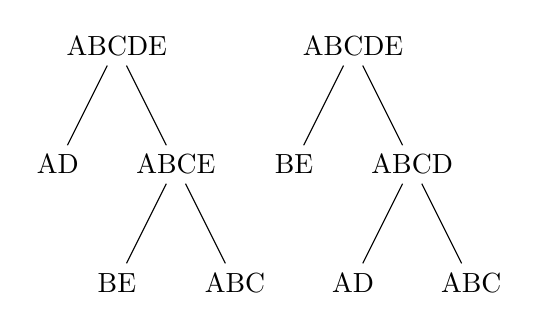
\begin{tikzpicture}
    \node (root1) at (0, 0) {ABCDE}
      child {node {AD}}
      child {node {ABCE}
        child {node {BE}}
        child {node {ABC}}};
    \node (root2) at (3, 0) {ABCDE}
      child {node {BE}}
      child {node {ABCD}
        child {node {AD}}
        child {node {ABC}}};
  \end{tikzpicture}
\end{figurebox}

Note that the decomposition that splits first $R[ABC]$ is not valid, since the resulting
relation $R[AB]$ is not a consequence of a functional dependency; see
\cref{fig:wrongdecomp}.

\begin{figurebox}[label=fig:wrongdecomp]{Invalid decomposition trees for the relation $R[ABCDE]$.}
  \centering
  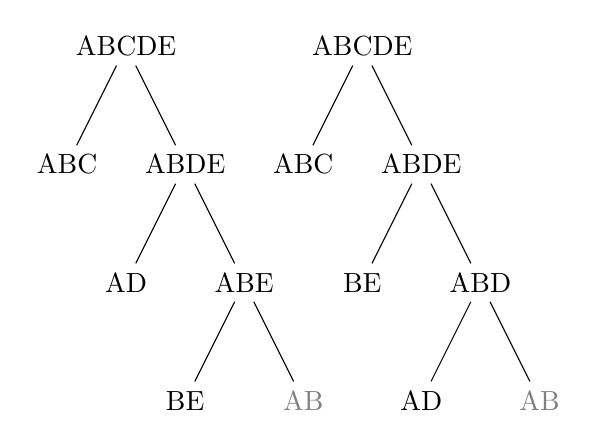
\begin{tikzpicture}
    \node (root1) at (0, 0) {ABCDE}
      child {node {ABC}}
      child {node {ABDE}
        child {node {AD}}
        child {node {ABE}
          child {node {BE}}
          child {node[gray] {AB}}}};
    \node (root2) at (3, 0) {ABCDE}
      child {node {ABC}}
      child {node {ABDE}
        child {node {BE}}
        child {node {ABD}
          child {node {AD}}
          child {node[gray] {AB}}}};
  \end{tikzpicture}
  \tcblower
  We consider the functional dependencies $A \to D$, $B \to E$, and $AB \to C$.
  Note that $R[AB]$ is not a consequence of a functional dependency.
\end{figurebox}

In this kind of relation schema, we have a set of key attributes, here $\mathcal{K} = AB$,
and a set of non-prime attributes, here $\mathcal{N} = CDE$.  Note that the case
$\mathcal{K} \cap \mathcal{N} = \emptyset$ is the simplest one we can have.

Observe, however, that transitive dependencies\footnote{Actually, when an attribute is
both key and non-prime, some joins may generate invalid tables.} and complex join
dependencies restrict even further the joins we are allowed to perform.
% \textcolor{red}{Further formalization and study is under progress.}

Now, consider a very common case: in our dataset, keys are unknown.  Let $A$ be a student
id, $B$ be the course id, $D$ be the student age, $E$ be the course load, and $C$ be the
student grade at the course.  If only $CDE$ is known, the table $R[CDE]$ is already tidy
--- and the observational unit is the enrollment --- once there is no key to perform any
kind of normalization.  This happens in many cases where privacy is a concern.

\begin{tablebox}[label=tab:student]{Example of a dataset where the observational unit is the student.}
  \centering
  \rowcolors{2}{black!10!white}{}
  \begin{tabular}{llll}
    \toprule
    \textbf{A (student)} & \textbf{B (course)} & \textbf{C (grade)} & \textbf{E (load)} \\
    \midrule
    1 & 1 & 7 & 60 \\
    1 & 2 & 8 & 30 \\
    2 & 1 & 7 & 60 \\
    2 & 3 & 9 & 40 \\
    \dots & \dots & \dots & \dots \\
    \bottomrule
  \end{tabular}
  \\[1em]
  \begin{tabular}{lll}
    \toprule
    \textbf{A (student)} & \textbf{F (average grade)} & \textbf{G (total load)} \\
    \midrule
    1 & 7.5 & 90 \\
    2 & 8 & 100 \\
    \dots & \dots & \dots \\
    \bottomrule
  \end{tabular}
  \tcblower
  Relation $R[ABCE]$ becomes $R[AFG]$ after the summarization operation.  Now each row
  represents a student (values in $A$ are unique).
\end{tablebox}

But we can also consider that the observational unit is the student.  In this case, we
must perform joins traversing the leftmost decomposition tree in \cref{fig:decomp} from
bottom to top.  After each join, a summarization operation is performed on the relation
considering the student as the observational unit, i.e., over attribute $A$.  The first
join results in relation $R[ABCE]$ and the summarization operation results in a new
relation $R[AFG]$ where $F$ is the average grade and $G$ is the total course load taken by
the student (see \cref{tab:student}).  They are all calculated based on the rows that are grouped in function of $A$.
It is important to notice that, after the summarization operation, all observations must
contain a different value of $A$.  The second join results in relation $R[ADFG] = R[AD]
\bowtie R[AFG]$.  This relation has functional dependency $A \to DFG$, and it is in 3NF
(which is also tidy).

Unfortunately, it is not trivial to calculate all possible decomposition trees for a given
dataset.  It is up to the data scientist to decide which directions to follow.  However,
it is important to notice that the order of the joins and summarization operations are
crucial to the final result.
%\textcolor{red}{Further formalization and study is under progress.}

\section{Data semantics and interpretation}

In the rest of the book, we focus on a statistical view of the data.  Besides the
functional dependencies, we also consider the statistical dependencies of the data.  For
instance, attributes $A$ and $B$ might not be functionally dependent, but they might exist
in an unknown $P(A, B)$ that we can estimate from the data.  Each observed value of a key can
represent an instance of a random variable, and the other attributes can represent
measured attributes or calculated properties.

For data analysis, it is very important to understand the relationships between the
observations.  For example, we might want to know if the observations are independent, if
they are identically distributed, or if there is a known selection bias.  We might also
want to know if the observations are dependent on time, and if there are hidden variables
that affect the observations.

Following wrong assumptions can lead to wrong conclusions.  For example, if we assume that
the observations are independent, but they are not, we might underestimate the variance of
the estimators.

Although we do not focus on time series, we must consider the temporal dependence of the
observations.  For example, we might want to know how the observation $x_t$ is affected by
$x_{t-1}$, $x_{t-2}$, and so on.  We might also want to know if the Markov property holds,
and if there is periodicity and seasonality in the data.

For the sake of the scope of this book, we suggest that any prediction on temporal data
should be done in the state space, where it is safer to assume that observations are
independent and identically distributed.  This is a common practice in reinforcement
learning and deep learning. Takens' theorem\footfullcite{Takens1980} allows you to
reconstruct the state space of a dynamical system using time-delay embedding. Given a
single observed time series, you can create a multidimensional representation of the
underlying dynamical system by embedding the time series in a higher-dimensional space.
This embedding can reveal the underlying dynamics and structure of the system.

\section{Unstructured data}

Unstructured data are data that do not have a predefined data model or are not organized
in a predefined manner.  For example, text, images, and videos are unstructured data.

Every unstructured dataset can be converted into a structured one.  However, the
conversion process is not always straightforward nor lossless.  For example, we can
convert a text into a structured dataset by counting the number of occurrences of each
word\footnote{This is called a bag-of-words approach.}.
However, we lose the order of the words in the text.

The study of unstructured data is, for the moment, out of the scope of this book.

% vim: set spell spelllang=en:

\chapter{Data handling}
\label{chap:handling}
\glsresetall

\chapterprecishere{%
  $\dagger$ It's dangerous to go alone! Take this.
  \par\raggedleft--- \textup{Unnamed Old Man}, The Legend of Zelda}

In the previous chapter, I discussed the relationship between data format and data
semantics.  We also saw in \cref{chap:project} that data tasks --- specifically
integration and tidying --- must adjust the available data to reflect the kind of
input we expect in production.  Data handling consists of operating on this data.

For those tasks, we must be careful with the operations we perform on the data. At the
stage of data preparation, for example, we should never parametrize our data handling
pipeline in terms of information retrieved\footnote{For instance, imputation by the mean
of a column.} by the values of the data.  This is because such operations lead to \gls{leakage}
during evaluation and other biases in our conclusions.

In this chapter, we consider that tables are rectangular data structures in which values
of the same column share the same properties (i.e. the same type, same restrictions, etc.)
and each column has a name.  Moreover, we assume that any value is possibly
\emph{missing}.

From a mathematical definition of such tables, we can define a set of operations that can
be applied to them.  These operations are the building blocks of data handling pipelines:
combinations of operations that transform a dataset into another dataset.

Finally, I highlight some important properties of these operations.  Especially, the
split-invariance property, which ensures that the operations do not add bias to the data
due to the way the data was collected.

\begin{mainbox}{Chapter remarks}

  \boxsubtitle{Contents}

  \startcontents[chapters]
  \printcontents[chapters]{}{1}{}
  \vspace{1em}

  \boxsubtitle{Context}

  \begin{itemize}
    \itemsep0em
    \item Data handling consists of operating on tables.
    \item Properties of the operations are important to avoid bias.
    \item Data handling pipelines are a way to organize these operations.
  \end{itemize}

  \boxsubtitle{Objectives}

  \begin{itemize}
    \itemsep0em
    \item Define a formal structure for tables.
    \item Define a set of operations that can be applied to tables.
  \end{itemize}

  \boxsubtitle{Takeaways}

  \begin{itemize}
    \itemsep0em
    \item Split-invariant operations avoid sampling bias.
    \item One must understand the properties and premises of the operations.
  \end{itemize}
\end{mainbox}

{}
\clearpage

\section{Formal structured data}
\label{sec:formal-structured-data}

\newcommand{\domainof}[1]{\mathcal{D}\!\left(#1\right)}
\newcommand{\missing}{\text{?}}
\newcommand{\rowcard}[1][k_1, \dots, k_k]{\operatorname{card}\!\left(#1\right)}

In this section, I present a formal definition of structured data.  This definition is
compatible with the relational model and tidy data presented in \cref{chap:data}.
My definition takes into account the index\footnote{Also called grouping variables.} of
the table, which is a key concept in data handling.  We also consider that values can be
missing.  Repeated rows are represented by allowing cells to contain sets of values.
In this chapter, we consider dataset and table as synonyms.

\begin{defbox}{Indexed table}{itable}
An indexed table $T$ is a tuple $(K, H, c)$, where $K = \left\{K_i : i = 1, \dots,
k\right\}$ is the set of index columns, $H$ is the set of (non-index) columns, and $c :
\domainof{K_1} \times \dots \times \domainof{K_k} \times H \to \mathcal{V}$ is the cell function.
Here, $\mathcal{V}$ represents the space of all possible tuples of values, which
may include missing values $\missing$.  Values have arbitrary types, such as integers,
real numbers, strings, etc.
Each index column $K_i$ has a domain $\domainof{K_i}$, which is an enumerable set of
values.
\end{defbox}

A possible row $r$ of the table is indexed by a tuple $r = (k_1, \dots,
k_k)$, where $k_i \in \domainof{K_i}$.  Each row has a cardinality $\rowcard[r]$, which
represents how many times the entity represented by the row is present in the table.
A row $r$ with $\rowcard[r] = 0$ is considered to be missing.

A cell is then represented by a row $r$ and a column $h \in H$.  The value of the cell,
$\vec{v} = c(r, h)$ is a tuple of values in the domain $\domainof{h} \cup \{\missing\}$,
such that $|\vec{v}| = \rowcard[r]$.  We say that $\domainof{h}$ is the valid domain of
the column $h$.
The order of the elements in the tuple $\vec{v}$ is arbitrary but fixed.

\begin{defbox}{Nested row}{nested-row}
A \emph{nested
row} consists of a tuple of values that associates different columns with the same
repetition of the entity, i.e. \[
  \Big[ v^h_i : h \in H \Big]\text{,}
\]
where $c(r, h) = [v^h_i : i = 1, \dots, \rowcard[r]]$, assuming an arbitrary fixed order
of the columns $h$.
\end{defbox}

We can stack nested rows to form a matrix of values.  This matrix is called the value
matrix of the row $r$.

\begin{defbox}{Value matrix}{vmatrix}
The value matrix $V = (v_{i, j})$ of the row $r$ is \[
  \Big[ c(r, h) : h \in H \Big]\text{,}
\] with dimensions $\rowcard[r] \times |H|$.
\end{defbox}

We assume that value matrices --- and consequently row cardinalities --- are minimal. This
means that there are no nested rows $$v_{i, 1}, \dots, v_{i, |H|}$$ in the value matrices
such that $v_{i, j} = \missing$ for all $j$.

From these concepts, we can define the basic operations and properties that can be applied
to tables.

\subsection{Splitting and binding}

Split and bind are very basic operations that can be applied to tables.  They are
inverses of each other and are used to divide and combine tables, respectively.
They are important in the data science process because they play a key role in
data semantics and validation of solutions.

\begin{defbox}{Split operation}{split}
Given an indicator function $s : \domainof{K_1} \times \dots \times \domainof{K_k} \to
\left\{0, 1\right\}$, the split operation creates two tables, $T_0$ and $T_1$, that
contain only the rows for which
$s(r) = 0$ and $s(r) = 1$, respectively.

Mathematically, the split operation is defined as \[
  \operatorname{split}(T, s) = \left(T_0, T_1\right)\text{,}
\] where $T = (K, H, c)$, $T_i = (K, H, c_i)$, and \[
  c_i(r, h) = \begin{dcases}
    c(r, h) & \text{if } s(r) = i \\
    () & \text{otherwise.}
  \end{dcases}
\]
\end{defbox}

\emph{Note that, by definition, the split operation never ``breaks'' a row.  So, the
indices define the indivisible entities of the table.}  The resulting tables are
disjoint:

\begin{defbox}{Disjoint tables}{disjoint-tables}
  Two tables $T_0 = (K, H, c_0)$ and $T_1 = (K, H, c_1)$ are said to be disjoint if
  $$\rowcard[r; c_0] > 0 \Rightarrow \rowcard[r; c_1] = 0\text{ and}$$
  $$\rowcard[r; c_1] > 0 \Rightarrow \rowcard[r; c_0] = 0$$ for any $r$.
\end{defbox}

The binding operation is the inverse of the split operation.

\begin{defbox}{Bind operation}{bind}
  Given two disjoint tables
  $T_0 = (K, H, c_0)$ and $T_1 = (K, H, c_1)$, the binding operation creates a new table $T$
  that contains all the rows of $T_0$ and $T_1$.

  Mathematically, the binding operation is defined as \[
    \operatorname{bind}(T_0, T_1) = (K, H, c)\text{,}
  \] where $T_i = (K, H, c_i)$ and \[ c(r, h) = c_0(r, h) + c_1(r, h)\text{.} \]
  The operator $+$ stands for the tuple concatenation operator%
  \footnote{The order of the concatenation here is not an issue since we guarantee
  that at least one of the operands is empty.}.
\end{defbox}

\emph{Thus, a requirement for the binding operation is that the tables are disjoint in
terms of the row entities they have.}

\paragraph{Premises in real-world applications}

One important aspect of these functions is that we assume that the entities represented by
the rows are indivisible, and that any binding operation will never occur for tables that
share the same entities.

In real-world applications, this is not always true.  Many times, we do not know the
process someone else has used to collect the data.  In these cases, we must be careful
about the guarantees we discuss in this chapter.  On the other hand, one can consider the
premises we use as a guideline to design good data collection processes.

We can see data collection as the result of a splitting operation in the universe set of
all possible entities.  This is a good way to think about data collection, as we can try
to ensure that we collect all possible information about the entities we are interested
in.

This, of course, depends on what we define as the index columns of the table.  Consider
the example of collecting information about grades of students.  If we define the student's
name and year as the indexes, we must ensure that we collect all the grades of all
subjects a student has taken in a year.  We do not need, though, to collect information
from all students or all years.  On the other hand, if we define only the student's name
as the index column, we must collect all the grades of all subjects a student has taken
in all years.

In summary, the fewer variables we define as index columns, the more information we must
collect about each entity.  However, in the next sections, we show that assuming many index columns
leads to restrictions in the operations we can perform on the table.

This conceptual trade-off is important to understand when structuring the problem we are
trying to solve.  Neglecting these issues can lead to strong statistical biases and
incorrect conclusions.

\subsection{Split invariance}

One property we can study about data handling operations is whether they are distributive
over the bind operation.  This property is called \emph{split invariance}.

From now on, we will denote \[
  T_0 + T_1 = \operatorname{bind}(T_0, T_1)\text{,}
\] for any tables $T_0$ and $T_1$ to simplify the notation.

\begin{defbox}{Split invariance}{split-invariance}
An arbitrary data handling operation $f(T)$ is said to be split-invariant
if, for any table $T$ and split function $s$, the following equation holds \[
  f\!\left(T_0 + T_1\right) =
    f\!\left(T_0\right) + f\!\left(T_1\right)\text{,}
\] where $T_0, T_1 = \operatorname{split}\!\left(T; s\right)$.
\end{defbox}

Split invariance is a desirable property for data handling operations during the data
tasks described in \cref{chap:project}: integration and tidying.  Even while exploring
data, we should take effort to use split-invariant operations.

The reason is that split invariance ensures that the operation does not depend on the
split performed (usually unknown to us) to create the table we have in hand.  This
property is important to avoid \gls{leakage} or to bias the results of the
analysis\footnote{Note that split invariance is a sufficient but not necessary condition
for preventing leakage.  Split invariance provides not only a ``safe by default''
guarantee, but also a way to pinpoint possible sources of leakage.}.

\subsection{Illustrative example}

\begin{tablebox}[label=tab:grades1]{Data table of student grades.}
  \centering
  \rowcolors{2}{black!10!white}{}
  \begin{tabular}{cccc}
    \toprule
    \textbf{student} & \textbf{subject} & \textbf{year} & \textbf{grade} \\
    \midrule
    Alice & Chemistry & 2020 & 6 \\
    Alice & Math & 2019 & 8 \\
    Alice & Physics & 2019 & 7 \\
    Bob & Chemistry & 2018 & ? \\
    Bob & Chemistry & 2019 & 7 \\
    Bob & Math & 2019 & 9 \\
    Bob & Physics & 2019 & 4 \\
    Bob & Physics & 2020 & 8 \\
    Carol & Biology & 2020 & 8 \\
    Carol & Chemistry & 2020 & 3 \\
    Carol & Math & 2020 & 10 \\
    \bottomrule
  \end{tabular}
  \tcblower
  Data collected about student grades.  All information that is available is presented.
\end{tablebox}

Consider the example of data collected about student grades.  \Cref{tab:grades1}
exemplifies all information we can possibly have about the grades of students.  A missing
value in a cell of that table indicates that, for some reason, the information is not
retrievable.

The domains of the variables are:
\begin{itemize}
  \itemsep0em
  \item $\domainof{\text{student}} = \left\{\text{Alice}, \text{Bob}, \text{Carol}\right\}$;
  \item $\domainof{\text{subject}} = \left\{\text{Biology}, \text{Chemistry}, \text{Math},
    \text{Physics}\right\}$;
  \item $\domainof{\text{year}} = \mathbb{Z}$; and
  \item $\domainof{\text{grade}} = \left[0, 10\right]$.
\end{itemize}

Of course, in practice, we have no guarantee that the data we have is complete nor a
clear specification of the domain of the variables.  Instead, we must choose good
premises about the data we are working with.

Knowing that the data is complete, we can safely assume that:
\begin{enumerate}
  \itemsep0em
  \item Alice has never taken Biology;
  \item Bob passed Physics, although at the second attempt;
  \item Carol has only taken classes in 2020.
\end{enumerate}

\begin{tablebox}[label=tab:grades2]{Data table of student grades assuming student and subject as indices.}
  \centering
  \rowcolors{2}{black!10!white}{}
  \begin{tabular}{ccccc}
    \toprule
    \textbf{s} & \textbf{student} & \textbf{subject} & \textbf{year} & \textbf{grade} \\
    \midrule
    0 & Alice & Chemistry & (2020) & (6) \\
    1 & Alice & Math & (2019) & (8) \\
    1 & Alice & Physics & (2019) & (7) \\
    0 & Bob & Chemistry & (2018, 2019) & (?, 7) \\
    0 & Bob & Math & (2019) & (9) \\
    1 & Bob & Physics & (2019, 2020) & (4, 8) \\
    0 & Carol & Biology & (2020) & (8) \\
    0 & Carol & Chemistry & (2020) & (3) \\
    1 & Carol & Math & (2020) & (10) \\
    \bottomrule
  \end{tabular}
  \tcblower
  Indexed table with data from \cref{tab:grades1} assuming student and
  subject as indices.  The column $s$ is the split indicator.
\end{tablebox}

Now consider an arbitrary collection mechanism that considers student and subject as the
indices of the table.  \Cref{tab:grades2} shows the table we have in hand.  The column $s$
is the split indicator.  Only rows with $s = 1$ are available to us.

Now, about the statements we made before:
\begin{enumerate}
  \itemsep0em
  \item There is no way we can know if Alice has taken Biology or not.  It could be that
    the data collection mechanism failed to collect this information or that the
    information simply does not exist.
  \item We can safely assume that Bob has passed Physics in his second attempt, once all
    information about (Bob, Physics) is assumed to be available.
  \item There is no guarantee that Carol has only taken classes in 2020.  It could be that
    some row (Carol, subject) with a year different from 2020 is missing in the table.
\end{enumerate}

\begin{tablebox}[label=tab:grades3]{Data table of student grades assuming student as the index.}
  \centering
  \rowcolors{2}{black!10!white}{}
  \begin{tabular}{ccp{2.6cm}p{1.8cm}>{\raggedright\arraybackslash}p{1.2cm}}
    \toprule
    \textbf{s} & \textbf{student} & \textbf{subject} & \textbf{year} & \textbf{grade} \\
    \midrule
    1 & Alice & (Chemistry, Math, Physics) & (2020, 2019, 2019) & (6, 8, 7) \\
    0 & Bob & (Chemistry, Chemistry, Math, Physics, Physics) & (2018, 2019, 2019, 2019, 2020) & (?, 7, 9, 4, 8) \\
    1 & Carol & (Biology, Chemistry, Math) & (2020, 2020, 2020) & (8, 3, 10) \\
    \bottomrule
  \end{tabular}
  \tcblower
  Indexed table with data from \cref{tab:grades1} assuming student
  as index.  The column $s$ is the split indicator and only rows with $s = 1$ are available to us.
\end{tablebox}

Now consider an arbitrary collection mechanism that considers student as the index of the table.
Imposing this restriction would difficult the data collection process, but it would
guarantee that we have all information about each student.  \Cref{tab:grades3} shows the
table we have in hand.  As before, the column $s$ is the split indicator and only rows with
$s = 1$ are available to us.

Our conclusions may change again:
\begin{enumerate}
  \itemsep0em
  \item We can safely assume that Alice has never taken the Biology class, as $\text{Biology}
    \not\in c(\text{Alice}, \text{subject})$.
  \item There is no information about Bob's grades, so we can not affirm nor deny anything
    about his grades.
  \item We can safely assume that Carol has only taken classes in 2020, as $c(\text{Carol},
    \text{year})$ contains only values with 2020.
\end{enumerate}

It is straightforward to see that the fewer index columns we have, the more information we
have about the present entities.  Also, it is clear how important the assumptions on the
index columns are to the conclusions we can draw from the data. Consequently,
split-invariant operations can preserve valid conclusions about the data even when
information is missing\footnote{Absence can be due to incomplete data collection or
artificial splitting for validation; consult \cref{chap:planning}.}.

\section{Data handling pipelines}

In the literature and in software documentation, you will find a variety of terms used to
describe data handling operations\footnote{%
  The terminology ``data handling'' itself is not universal.  Some authors and libraries
  call it ``data manipulation'', ``data wrangling'', ``data shaping'', or ``data
  engineering''.  I use the term ``data handling'' because it seems more generic.
  Also, it avoids confusion with the term ``data
  manipulation'' which has a negative connotation in some contexts.}. %
They often refer to the same or similar operations, but the terminology can be confusing.
In this section, I present a summary of these operations mostly based on
\textcite{Wickham2023} definitions\footnote{Which they call \emph{verbs}.}.


During the preparation of data for our project, we will need to perform a set of operations
on possibly multiple datasets.  These operations are organized in a pipeline, where the
outputs of one operation are the inputs of the next one.
Operations are extensively parameterized, for instance, most of them can use predicates to
define the groups, arrangements, or conditions under which they should be applied.

\begin{figurebox}[label=fig:pipeline]{Example of data handling pipeline.}
  \centering
  \begin{tikzpicture}[every node/.style={font=\small, inner sep=4pt}]
    \node (s1) [darkcircle] at (0, 0) {Source 1};
    \node (s2) [darkcircle] at (0, -2) {Source 2};
    \node (f1) [mediumblock] at (2, 0) {$f_1$};
    \node (f2) [mediumblock] at (4, 0) {$f_2$};
    \node (f3) [mediumblock] at (2, -2) {$f_3$};
    \node (f4) [mediumblock] at (4, -2) {$f_4$};
    \node (f5) [mediumblock] at (6, -1) {$f_5$};
    \node (data) [darkcircle, minimum width=15mm] (data) at (8, -1) {Data};

    \path [line] (s1) -- (f1);
    \path [line] (f1) -- (f2);
    \path [line] (f1.east) -- (f4);
    \path [line] (s2) -- (f3);
    \path [line] (f3) -- (f4);
    \path [line] (f2) -- (f5);
    \path [line] (f4) -- (f5);
    \path [line] (f5) -- (data);
  \end{tikzpicture}
  \tcblower
  A data handling pipeline is a set of operations that transform a dataset into
  another dataset.  We can have more than one source dataset and the output is a single
  dataset where each row represents a sample in the observational unit we are interested
  in.
\end{figurebox}

In \cref{fig:pipeline}, we show an example of a data handling pipeline.  The pipeline
starts with two source datasets, Source 1 and Source 2.  The datasets are processed by a
set of operations, $f_1, f_2, f_3, f_4, f_5$, and the output is a single dataset,
Data.  Our goal at the data tasks --- see \cref{sub:workflow} --- is to create a dataset
that is representative of the observational unit we are interested in.  Representative
here means that the dataset is tidy\footnote{Remember that our definition of tidiness
depends on the observational unit.  That means, in practice, that if the original data
sources are in a observational unit different from the one we are interested in, after
joining them, the connecting variables may need to be removed to eliminate transitive
dependencies.  Consult \cref{sub:tidy-not-tidy,sub:change-unit}.} and that the priors,
i.e. the distribution of the data is faithful to the real distribution of the phenomenon.

A pipeline is more flexible than a chain of operations because it can handle more complex
structures, where different branches (forks) of processing occur simultaneously, and then
come together (merges) later in the workflow.  For instance, the output of $f_1$ is the
input of $f_2$ and $f_4$ (fork), and $f_5$ has as input the outputs of $f_2$ and $f_4$
(merge).

Pipelines are great conceptual tools to organize the data handling process.  They allow
for the separation of concerns, where each operation is responsible for a single task.
Also, declaring the whole pipeline at once allows for the optimization of the operations
and the use of parallel processing.  This is important when dealing with large datasets.
The declarative approach, as opposed to the imperative one, makes it easier to reason about
and maintain the code\footnote{Tidyverse and Polars are examples of
libraries that use a declarative approach to data handling.}.

\section{Split-invariant operations}
\label{sec:split-invariant-ops}

In this section, I present a set of operations that are split-invariant.  One can safely
apply these operations to the data without worrying about biasing the dataset.

For each operation, we discuss its application on some tidying issues presented in
\cref{sub:messy}.  The issues I address here\footnote{%
The issue of multiple types of observational units stored in the same table is better
dealt with by database normalization.  More on this subject is discussed in
\cref{sub:projection}.}:
\begin{itemize}
  \itemsep0em
  \item Headers are values, not variable names;
  \item Multiple variables are stored in one column; % [mutate/select problem]
  \item Variables are stored in both rows and columns;
  \item A single observational unit is stored in multiple tables.
\end{itemize}



\subsection{Tagged splitting and binding}

We saw that one trivial, yet important, operation is to bind datasets.  This is the
process of combining two or more datasets into a single dataset.  To make the
operation reversible, we can parametrize it with a split column that indicates the source
of each row.

\begin{defbox}{Tagged bind operation}{tagged-bind}
  Given two or more disjoint tables $T_i = (K, H, c_i)$, $i = 0, 1, \dots$, the tagged
  bind operation creates a new table $T = (K, H \cup \{s\}, c)$ that contains all the rows
  of tables $T_i$.  The split column $s$ is a new column that indicates the source of each
  row.

  Mathematically, the tagged bind operation is defined as \[
    \operatorname{bind}_{s}(T_0, T_1, \dots) = T\text{,}
  \] where $c(r, h) = c_0(r, h) + c_1(r, h) + \dots$ if $h \in H$ and \[
    c(r, s) = \left[ i \right]^{d} \text{,}
  \]
  where $i$ is the index of the table $T_i$ that contains the row $r$, i.e. $d =
  \rowcard[r; c_i] > 0$.
\end{defbox}

When binding datasets by rows, the datasets must have the same columns.  In practice,
one can assume, if a column is missing, that all values in that column are missing.

The indication of the source table usually captures some hidden semantics that has split
the tables in the first place. For instance, if each table represents data collected in a
different year, one can create a new column \emph{year} that contains the year of the
data.  It is important to pay attention to the semantics of the split column, as it can
also contain extra information.

\begin{tablebox}[label=tab:gas-usage]{Gas usage datasets.}
  \centering
  \rowcolors{2}{black!10!white}{}
  \begin{tabular}{ccc}
    \toprule
    \textbf{month} & \textbf{gas} & \textbf{distance} \\
    \midrule
    1 & 48.7 & 1170 \\
    2 & 36.7 & 1100 \\
    3 & 37.8 & 970 \\
    \dots & \dots & \dots \\
    \bottomrule
  \end{tabular}
  ~
  \rowcolors{2}{black!10!white}{}
  \begin{tabular}{ccc}
    \toprule
    \textbf{month} & \textbf{gas} & \textbf{distance} \\
    \midrule
    1 & 143.7 & 1470 \\
    2 & 156.7 & 1700 \\
    3 & 170.8 & 1870 \\
    \dots & \dots & \dots \\
    \bottomrule
  \end{tabular}
  \tcblower
  Monthly gas usage data from US (left) and Brazil (right) residents.
\end{tablebox}

Consider \cref{tab:gas-usage}, which contains monthly gas usage data from
US and Brazil residents.  From the requirements described in the previous section, we can
safely bind these datasets --- as they are disjoint.  We can use as a tag a new column to
represent the country.  However, an attentive reader will notice that the unit of
measurement of the gas usage and distance are different in each table: gallons and miles
in the US dataset and liters and kilometers in the Brazil dataset.  Ideally, thus, we
should create two other columns to represent the units of measurement.

It is straightforward to see that this operation solves the issue of a single
observational unit being stored in multiple tables described in \cref{sub:messy}.

The reverse function consists of splitting the dataset using as a predicate the split column.

\begin{defbox}{Tagged split operation}{tagged-split}
  Let $s$ be a non-index column of a table $T = (K, H \cup \{s\}, c)$ with $\domainof{s}$
  known and finite, and such that $c(r, s)$ contains only unique values. The tagged split
  operation parametrized by $s$ creates disjoint tables $T_i = (K, H, c_i)$ that contain
  only the rows $r$ for which $c(r, s) = i$.

  Mathematically, the tagged split operation is defined as \[
    \operatorname{split}_{s}(T) = \left(T_0, T_1, \dots\right)\text{,}
  \] where $c_i(r, h) = c(r, h)$ if $i \in c(r, s)$ and $c_i(r, h) = ()$ otherwise.
\end{defbox}

Note that the tagged split is split-invariant by definition, since we assume that the
nested rows of the input table $T$ contain only one value for column $s$ for all
rows\footnote{We consider a slightly different definition of split invariance here, where
the binding operation is applied to each element of the output of the split operation.}.
Failing to meet this assumption can lead to a biased split.  Also, in practice, it is
good practice to keep the column $s$ in the output tables to preserve information about
the source of the rows.  In terms of storage, smart strategies can be used to avoid the
unnecessary repetition of the same value in column $s$.

\subsection{Pivoting}

Another important operation is pivoting datasets.  There are two types of pivoting:
long-to-wide and wide-to-long.  These operations are reversible and are the inverse
of each other.

Pivoting long-to-wide requires a name column --- whose discrete and finite
possible values will become the names of the new columns --- and a value column --- whose
values will be \emph{spread} across the rows.  Other than these columns, all remaining columns
must be indexes.

\begin{defbox}{Pivot long-to-wide operation}{pivot-l2w}
  Let $T = (K \cup \{\text{name}\}, \{\text{value}\}, c)$. The pivot long-to-wide
  operation is defined as \[
    \operatorname{pivot}_\text{name}(T) = T'\text{,}
  \] where $T' = (K, \domainof{\text{name}}, c')$ and \[
    c'(r, h) = c\left(r + (h),~\text{value}\right)\text{,}
  \]
  for all valid row $r$ and $h \in \domainof{\text{name}}$.
\end{defbox}

Note however that the operation only works if $\rowcard[r + (h); c]$ is constant for all
$h \in \domainof{\text{name}}$.  If this is not the case, one must aggregate the rows
before applying the pivot operation.  This is discussed in \cref{sub:aggregation}.

Pivoting wide-to-long\footnote{Also known as unpivot.} is the reverse operation. One must
specify all the columns whose names are the values of the previously called ``name column.''
The values of these columns will be \emph{gathered} into a new column. As before, all
remaining columns are indexes.

\begin{defbox}{Pivot wide-to-long operation}{pivot-w2l}
  Let $T = (K, H, c)$ be a table.  The pivot wide-to-long
  operation is defined as \[
    \operatorname{pivot}^{-1}(T) = T'\text{,}
  \] where $T' = (K \cup \{\text{name}\}, \{\text{value}\}, c')$, $\domainof{\text{name}}
  = H$ and \[
    c'((r, h), \text{value}) = c(r, h)\text{,}
  \] for all valid row $r$ and $h \in H$.
\end{defbox}

In practical applications, where not all remaining columns are indexes, one must aggregate
rows or drop extra non-indexed columns beforehand.  This is discussed in
\cref{sub:aggregation,sub:selection}.

\begin{tablebox}[label=tab:pivot]{Pivoting example.}
    \centering
    \rowcolors{2}{black!10!white}{}
    \begin{tabular}{ccc}
      \toprule
      \textbf{city} & \textbf{year} & \textbf{qty.} \\
      \midrule
      A & 2019 & 1 \\
      A & 2020 & 2 \\
      A & 2021 & 3 \\
      B & 2019 & 4 \\
      B & 2020 & 5 \\
      B & 2021 & 6 \\
      \bottomrule
    \end{tabular}
    ~
    \rowcolors{2}{black!10!white}{}
    \begin{tabular}{cccc}
      \toprule
      \textbf{city} & \textbf{2019} & \textbf{2020} & \textbf{2021} \\
      \midrule
      A & 1 & 2 & 3 \\
      B & 4 & 5 & 6 \\
      \bottomrule
    \end{tabular}
  \tcblower
  The left-hand-side table is in the long format and the right-hand-side table is in the
  wide format.
\end{tablebox}

\Cref{tab:pivot} shows an example of pivoting.  Here, we can consider \emph{city} and
\emph{year} as the index columns.  The left-hand-side table is in the long format and the
right-hand-side table is in the wide format.  Using the pivot long-to-wide operation with
\emph{year} as the name column and \emph{qty.} as the value column, we can obtain the
right-hand-side table.  The reverse operation will give us the left-hand-side table.

To show that the pivot operation is split-invariant, one can see that, given
$T_0 = (K, H, c_0)$ and $T_1 = (K, H, c_1)$ disjoint tables,
\[
  \operatorname{pivot}_\text{name}\!\left(T_0\right) + \operatorname{pivot}_\text{name}\!\left(T_1\right) = \\
    (K, \domainof{\text{name}}, c_0') + (K, \domainof{\text{name}}, c_1')\text{,}
\] where $c_i'(r, h) = c_i(r + (h), \text{value})$.  However, by the disjoint property of
the tables, we have that \[
  c_0(r + (h), \text{value}) + c_1(r + (h), \text{value}) = c(r + (h), \text{value})\text{,}
\] for the table $T = (K, H, c) = T_0 + T_1$. So,
\begin{multline*}
  (K, \domainof{\text{name}}, c_0') + (K, \domainof{\text{name}}, c_1') =
    (K, \domainof{\text{name}}, c') =\\
    \operatorname{pivot}_\text{name}\!\left(T\right)\text{,}
\end{multline*}
where $c'(r, h) = c(r + (h), \text{value})$.

Similarly, the reverse operation is also split-invariant.

Using the pivot operation, we can solve the issues of headers being values, not variable
names and variables being stored in both rows and columns.  In the first case, we can pivot
the table to have the headers as the domain of a new index (name column).  In the second
case, we have to pivot both long-to-wide and wide-to-long to solve the issue.

\subsection{Joining}

Joining is the process of combining two datasets into a single dataset based on common
columns.  This is one of the two fundamental operations in relational algebra. We will see
the conditions under which the operation is split invariant. However, the join operation
has some other risks you should be aware of; consult \cref{sec:normalization} for more
details.

Adapting the definitions of join in our context, we can define it as follows.
For the sake of simplicity, we denote $r[U]$ as the row $r$ restricted to the index
columns in $U$, i.e.
\begin{equation*}
  % \label{eq:row-subscript}
  r[U] = (k_i : k_i \in \domainof{K_i} \forall K_i \in U)\text{.}
\end{equation*}

\begin{defbox}{Join operation}{join}
  Let $T' = (K', H', c')$ and $T'' = (K'', H'', c'')$ be two tables such that $K'
  \cap K'' \neq \emptyset$ and $H' \cap H'' = \emptyset$.  The join operation is
  defined as \[
    \operatorname{join}(T', T'') = T\text{,}
  \] where $T = (K' \cup K'', H' \cup H'', c)$ and \[
    c(r, h) = ()
  \] if $\rowcard[{r[K']; c'}] = 0$ or $\rowcard[{r[K'']; c''}] = 0$, for all $h$.
  Otherwise: \[
    c(r, h) = \begin{dcases}
      c'(r[K'], h) & \text{if } h \in H'\text{,} \\
      c''(r[K''], h) & \text{if } h \in H''\text{.}
    \end{dcases}
  \]
\end{defbox}

The join of two tables is the operation that returns a new table with the columns of both
tables.  Let $U$ be the common set of index columns.  For each occurring value of $U$ in
the first table, the operation will look for the same value in the second table.  If it
finds it, it will create a new row with the columns of both tables.  If it does not find
it, no row will be created.

Note that, like in pivoting long-to-wide, one must ensure that the cardinality of the
joined rows is constant for all $h \in H' \cup H''$.  If this is not the case, one must
aggregate the rows before applying the join operation.  This is discussed in
\cref{sub:aggregation}.

Before we discuss whether the join operation is split-invariant\footnote{Note that up to
this point, we have defined this property only for unary operations.}, we can discuss a
variation of the join operation: the left join.  The left join is the same as the join
operation, but if the value of $U$ is missing in the second table, the operation will
create a new row with the columns of the first table and missing values for the columns of
the second table.

In our context, this operation is a unary operation, where the second table is
a fixed parameter.

\begin{defbox}{Left join operation}{left-join}
  Let $T' = (K', H', c')$ and $T'' = (K'', H'', c'')$ be two tables such that $K'
  \cap K'' \neq \emptyset$ and $H' \cap H'' = \emptyset$.  The left join operation is
  defined as \[
    \operatorname{join}(T'; T'') = \operatorname{join}_{T''}(T') = T\text{,}
  \] where $T = (K' \cup K'', H' \cup H'', c)$ and \[
    c(r, h) = ()
  \] if $\rowcard[{r[K']; c'}] = 0$ for all $h$. Otherwise:
  \[
    c(r, h) = \begin{dcases}
      c'(r[K'], h) & \text{if } h \in H'\text{,} \\
      c''(r[K''], h) & \text{if } h \in H''\text{.}
    \end{dcases}
  \]
\end{defbox}

The left join operation is split-invariant.  To see this, consider two disjoint tables
$T_0 = (K, H, c_0)$ and $T_1 = (K, H, c_1)$, and a third table $T' = (K', H', c')$ such
that $K \cap K' \neq \emptyset$ and $H \cap H' = \emptyset$.  We have that
\begin{multline*}
  \operatorname{join}_{T'}(T_0) + \operatorname{join}_{T'}(T_1) =
  T_0' + T_1' =\\
    (K \cup K', H \cup H', c_0') + (K \cup K', H \cup H', c_1')\text{,}
\end{multline*}
where the meaning of each term is clear from the \cref{def:left-join}.
It is straightforward to see that rows in $T_0'$ and $T_1'$ are disjoint, since at least
part of the indices in $K \cup K'$ are different between them.

Moreover, \[
  \operatorname{join}_{T'}(T_0 + T_1) = (K \cup K', H \cup H', c')
\] with $c'(r, h) = ()$ only if both $\rowcard[{r[K]; c_0}] = 0$ and $\rowcard[{r[K];
c_1}] = 0$.  Otherwise, $c'(r, h) = c_0(r[K], h) + c_1(r[K], h)$ if $h \in H$ and $c'(r,
h) = c_0(r[K], h)$ if $h \in H'$.

Thus, \[
  \operatorname{join}_{T'}(T_0 + T_1) = \operatorname{join}_{T'}(T_0) + \operatorname{join}_{T'}(T_1)\text{.}
\]

Our conclusion is that the left join operation given a fixed table is split-invariant.
So we can safely use it to join tables without worrying about biasing the dataset once we
fix the second table.

I conjecture that the (inner) join operation shares similar properties but it is not as
safe; nonetheless, a clear definition of split invariance for binary operations is needed.
This is left as a thought exercise for the reader.  Notice that the traditional join has
the ability to ``erase'' rows from any of the tables involved in the operation.  This is a
potential source of bias in the data.  This further emphasizes the importance of
understanding the semantics of the data schema before joining tables --- consult
\cref{sec:normalization}.

\subsection{Selecting}
\label{sub:selection}

Selecting is the process of choosing a subset of non-index columns from a dataset.  The
remaining columns are discarded.  Rows of the table remain unchanged.

Although very simple, the selection operation is useful for removing columns that are not
relevant to the analysis.  Also, it might be needed before other operations, such as
pivoting, to avoid unnecessary columns (wide-to-long) and to keep only the value column
(long-to-wide).

\begin{defbox}{Selection operation}{selection}
  Let $T = (K, H, c)$ be a table and $H' \subseteq H$.  The selection operation is
  defined as \[
    \operatorname{select}_{H'}(T) = T'\text{,}
  \] where $T' = (K, H', c)$.
\end{defbox}

Sometimes, it is useful to select columns based on a function of the column properties.
In other words, the selection operation can be parameterized by a predicate.  The predicate
is a function that returns a logical value given the column.

\begin{defbox}{Predicate selection operation}{predicate-selection}
  Let $T = (K, H, c)$ be a table and $P : H \to \{0, 1\}$ be a predicate.  The predicate
  selection operation is defined as \[
    \operatorname{select}_{P}(T) = T'\text{,}
  \] where $T' = (K, H', c)$ and $H' = \{h \in H : P(h) = 1\}$.
\end{defbox}

It is trivial to see that, if $P$ does not depend on the values of the columns (i.e., has no
access to $c$), the predicate selection operation is split-invariant.  This is because the
operation does not change the rows of the table nor does it depend on the values of the rows.

One example of the use of the predicate selection operation is to keep columns whose
values are in a specific domain.  For instance, to keep only columns that contain real
numbers, we choose $P(h) = 1$ if $\domainof{h} = \mathbb{R}$, and $P(h) = 0$ otherwise.

The case where the predicate depends on the values of the columns is discussed in
\cref{sub:grouped-arranged}.

\subsection{Filtering}
\label{sub:filtering}

Filtering is the process of selecting a subset of rows from a dataset based on a
predicate.

A predicate can be a combination of other predicates using logical operators, such as
logical disjunction (or) or logical conjunction (and).  In the general case, predicates
need to be robust enough to deal with value matrices of any size and those that contain missing
values.

After filtering, the dataset will contain only the rows that satisfy the predicate.
Columns remain unchanged.

In its simplest form, we can assume that $\rowcard[r] \leq 1$ for all $r$ and that the
predicates are applied to each row independently.  In this case, the value matrix $V(r)$
is just a tuple with a single value for each non-index column.

Without loss of generality, we can assume that predicates are combined using logical
disjunction (or)\footnote{The reason is that sequential application of filtering is
equivalent to combining the predicates using logical conjunction (and).}.

For instance, the predicate \code{age > 18} will select all rows where the value in the
age column is greater than 18.  Keeping each row independent, we can also generalize
predicates to deal with the values of the indexes as well.

\begin{defbox}{Filtering operation}{filtering}
  Let $T = (K, H, c)$ be a table and $P_1, \dots P_n$ be predicates.  The
  filtering operation is defined as \[
    \operatorname{filter}_{P_1, \dots, P_n}(T) = T'\text{,}
  \] where $T' = (K, H, c')$ and \[
    c'(r, h) = \begin{dcases}
      c(r, h) & \text{if } \bigvee_{i = 1}^{n} P_i(r, V(r)) = 1\text{,} \\
      () & \text{otherwise}\text{,}
    \end{dcases}
  \] where predicate $$P_i : \bigtimes_{K_i} K_i \times
  \bigtimes_{h\in H}\left(\domainof{h} \cup \{?\}\right) \to \{0, 1\}$$ is applied to the value
  matrix $V(r)$ of the row $r$.
\end{defbox}

It is also trivial to see that the filtering operation is split-invariant, even in its
generalized form where the value matrix has many rows.  This property comes from the fact
that rows are treated independently.  More complex cases are discussed in
\cref{sub:grouped-arranged}.

\subsection{Mutating}

Mutating is the process of creating new columns in a table.  The operation is reversible,
as the original columns are kept.  The new columns are added to the dataset.

The values in the new column are determined by a function of the rows.  The expression is
a function that returns a vector of values given the values in the other columns.
Similarly to filtering, in its simplest form, we can assume that $\rowcard[r] \leq 1$ for
all $r$ and that the predicates are applied to each row independently.

\begin{defbox}{Mutation operation}{mutating}
  Let $T = (K, H, c)$ be a table and $f$ be a transformation function.  The mutating
  operation is defined as \[
    \operatorname{mutate}_{f}(T) = T'\text{,}
  \] where $T' = (K, H \cup \{ h' \}, c')$ and \[
    c'(r, h) = \begin{dcases}
      c(r, h) & \text{if } h \in H\text{,} \\
      f(r, V(r)) & \text{if } h = h'\text{,}
    \end{dcases}
  \] where the function $$f : \bigtimes_{K_i \in K} K_i \times \bigtimes_{h\in H}
  \left(\domainof{h} \cup \{?\}\right) \to \domainof{h'} \cup \{?\}$$ is applied to the
  value matrix $V(r)$ of the row $r$.
\end{defbox}

The expression can be a simple function, such as \code{y = x + 1}, or a more complex
function, such as
\begin{center}
  \code{y = ifelse(x > 0, 1, 0)}.
\end{center}
Here, x and y are the names of an existing and the new column, respectively. The
\code{ifelse(a, b, c)} function is a conditional function that returns 1 if the condition
is true and 0 otherwise.

This function solves the issue of multiple variables stored in one column described in
\cref{sub:messy}.

As with filtering, the mutating operation is split-invariant even if $\rowcard[r] > 1$ for
any $r$\footnote{It just changes the input space of function $f$.}.  This is because the
operation is applied to each row independently.  In this general case, an extra
requirement is that the function $f$ must return tuples with the same cardinality as
the row it is applied to.

\subsection{Aggregating}
\label{sub:aggregation}

Many times, it is easier to reason about the table when all rows have cardinality 1.
Aggregation ensures that the table has this property.

\begin{defbox}{Aggregation operation}{aggregating}
  Let $T = (K, H, c)$ be a table and $f$ be an aggregation function.  The aggregation
  operation is defined as \[
    \operatorname{aggregate}_{f}(T) = T'\text{,}
  \] where $T' = (K, H, c')$ and \[
    c'(r, h) = f(r, V(r))[h]\text{,}
  \] where function $f$ is applied to the value matrix $V(r)$ of the row $r$ and it has
  an image $$\left(\domainof{h} \cup \{?\} : h \in H\right)\text{,}$$ independently of the
  input size.  The notation $v[h]$ refers to the value corresponding to the column $h$ in the
  output tuple.
\end{defbox}

As with mutation, aggregation is split-invariant as it treats each row independently,
even if the function $f$ considers order semantics of the values in the matrix.

\subsection{Ungrouping}
\label{sub:ungrouping}

We discussed that the fewer index columns a table has ---
assuming we guarantee that all information about that entity is present --- the safer
it is to infer conclusions from the data.  Thus, reducing the number of indices
must be done very carefully --- more on that in \cref{sub:projection}.

On the other hand, sometimes it is useful to increase the number of index columns.  For
instance, pivoting long-to-wide requires all columns except one to be indexes.  The
operation that transforms some of the columns in the table into indexes is called ungrouping.
The reason for the name is that the operation decreases the cardinality of rows
by creating new rows, effectively ungrouping the values.

\begin{defbox}{Ungrouping operation}{grouping}
  Let $T = (K, H, c)$ be a table and $h' \in H$ such that $\domainof{h'}$ is known and
  finite.  The ungrouping operation is defined as \[
    \operatorname{ungroup}_{h'}(T) = T'\text{,}
  \] where $T' = (K \cup \{h'\}, H \setminus \{h'\}, c')$, and \[
    c'(r + r', h) = (v_{i,h} : i)\text{,}
  \] where $r$ refers to values of the indices in $K$, $r'$ refers to the value of the new index
  $h'$, and $v_{i,h}$ is the value of the column $h$ in any $i$-th nested row of the value
  matrix $V(r; T)$ in the original table such that \[
    v_{i, h'} = r'\text{.}
  \]
\end{defbox}

Note that the operation requires that the column $h'$ has no missing values.

\begin{tablebox}[label=tab:ungroup]{Ungrouping example.}
  \centering
  \rowcolors{2}{black!10!white}{}
  \begin{tabular}{ccc}
    \toprule
    \textbf{city} & \textbf{year} & \textbf{qty.} \\
    \midrule
    A & (2019, 2020, 2020, 2021) & (1, 2, 3, 4) \\
    B & (2019, 2020, 2021) & (5, 6, 7) \\
    \bottomrule
  \end{tabular}

  \vspace{1em}
  \rowcolors{2}{black!10!white}{}
  \begin{tabular}{ccc}
    \toprule
    \textbf{city} & \textbf{year} & \textbf{qty.} \\
    \midrule
    A & 2019 & 1 \\
    A & 2020 & (2, 3) \\
    A & 2021 & 4 \\
    B & 2019 & 5 \\
    B & 2020 & 6 \\
    B & 2021 & 7 \\
    \bottomrule
  \end{tabular}
  \tcblower
  The index of the top table is the column \emph{city}.  The bottom table is the result of
  ungrouping the column \emph{year}.
\end{tablebox}

\Cref{tab:ungroup} shows an example of ungrouping.  In the top table, there are two rows,
one with cardinality 4 and the other with cardinality 3.  The column \emph{year} is
ungrouped, creating new rows for each value in the nested row.  The bottom table is the
result of ungrouping the column \emph{year}.  Although there were 7 nested rows in the
original table, the bottom table has 6 rows --- the number of nested rows is preserved
however.  The reason is that the row (A, 2020) has cardinality 2.

The ungrouping operation is split-invariant.  To see this, consider two disjoint tables
$T_0 = (K, H, c_0)$ and $T_1 = (K, H, c_1)$, we have
\begin{multline*}
  \operatorname{ungroup}_{h'}(T_0) + \operatorname{ungroup}_{h'}(T_1) = \\
    \left(K \cup \{h'\}, H \setminus \{h'\}, c_0'\right) +
    \left(K \cup \{h'\}, H \setminus \{h'\}, c_1'\right)\text{,}
\end{multline*}
where $c_j'(r + r', h) = (v_{i,h} : i \text{ such that } v_{i, h'} = r')$. Since the
tables are disjoint, the rows of the output tables are also disjoint.  In other words,
For any $r$, either $\rowcard[{r + r'; c_0}] = 0$ or $\rowcard[{r + r'; c_1}] = 0$
independently of the value of $r'$.  The reason is that there is no possible $v_{i,h'} =
r'$ if $r$ is not present in the table.

Then,
\begin{multline*}
  \left(K \cup \{h'\}, H \setminus \{h'\}, c_0'\right) +
  \left(K \cup \{h'\}, H \setminus \{h'\}, c_1'\right) = \\
    \left(K \cup \{h'\}, H \setminus \{h'\}, c'\right)\text{,}
\end{multline*}
where $c'(r + r', h) = c_0'(r + r', h) + c_1'(r + r', h)$.

\section{Other operations}

We saw that, under reasonable premises, split-invariant operations are safe to use in the
context of tidying and data integration.  However, data handling does not happen only in
the context of tidying and integrating datasets\footnote{And, sometimes, we may need to
use other transformations even for these tasks.}.  It is also used in tasks like data
exploration and data preprocessing.  In these cases, other operations are needed.

In this section, we discuss some of these operations.  Instead of focusing on the
mathematical definitions, we will discuss the semantics of the operations and some
of their properties.

\subsection{Projecting or grouping}
\label{sub:projection}

Projection is one of the two fundamental operations in relational algebra --- consult
\cref{sec:normalization} for more details.  In database normalization theory, tables ---
called relations --- are slightly different from the tables we are discussing here. The
major difference is that they are sets of tuples, which means that each tuple is unique.
In our scenario, this is similar to what we call rows represented by the possible values
of the index columns of the table.

Adapting the definitions of projection to our context, we can define it as follows.

\begin{defbox}{Projection operation}{projection}
  Let $T = (K, H, c)$ be a table and $K' \subset K$ a subset of the columns.  The
  projection operation is defined as \[
    \operatorname{project}_{K'}(T) = T'\text{,}
  \] where $T' = (K', H \cup (K \setminus K'), c')$ and \[
    c'(r, h) = \begin{dcases}
      \sum_{r'} c(r + r', h) & \text{if } h \in H \\
      \sum_{k' \in \domainof{h}} k' & \text{if } h \in K \setminus K'\text{,}
    \end{dcases}
  \] for all valid row $r$ considering the indices $K'$ and for all tuples $r' = (k_i :
  i)$ such that $k_i \in \domainof{K_i}$ for all $K_i \in K \setminus K'$.
\end{defbox}

We can see that projection for our tables is a little more complex than the usual
projection in relational algebra.  Consider the example we discussed in
\cref{sec:normalization} as well, where we have a table with the columns \emph{student},
\emph{subject}, \emph{year}, and \emph{grade}.

\begin{tablebox}[label=tab:student-grade-handling]{Student grade table.}
  \centering
  \rowcolors{2}{black!10!white}{}
  \begin{tabular}{cccc}
    \toprule
    \textbf{student} & \textbf{course} & \textbf{course credits} & \textbf{grade} \\
    \midrule
    Alice & Math & 4 & A \\
    Alice & Physics & 3 & B \\
    Bob & Math & 4 & B \\
    Bob & Physics & 3 & A \\
    Carol & Math & 4 & C \\
    \bottomrule
  \end{tabular}

  \vspace{1em}
  \rowcolors{2}{black!10!white}{}
  \begin{tabular}{cccc}
    \toprule
    \textbf{course} & \textbf{student} & \textbf{course credits} & \textbf{grade} \\
    \midrule
    Math & (Alice, Bob, Carol) & (4, 4, 4) & (A, B, C) \\
    Physics & (Alice, Bob, Carol) & (3, 3, ?) & (B, A, ?) \\
    \bottomrule
  \end{tabular}
  \tcblower
  (Top) An example of a table of students and their grades in courses.  The columns
  \emph{student} and \emph{course} are the index columns. (Bottom) The same table
  projected into the entity \emph{course}.
\end{tablebox}

\Cref{tab:student-grade-handling} (top) shows that table adapted for our definitions.
Suppose we want to project the table to have only the entity \emph{course}.
Now each row (bottom table) represents a course.  The column \emph{student} is not an
index column anymore, and the values in the column are exhaustive and unique, i.e.,
the whole set $\domainof{\text{student}}$ is represented in the column for each row.

Thus, projection is a very useful operation when we want to change the observational unit
of the data, particularly to the entity represented by a subset of the index columns.
Semantically, projection groups the rows by the values.

It is easy to see that the projection operation is not split-invariant.  Consider the
following example. If we split the top table in \cref{tab:student-grade-handling} so the
first row (Alice, Math) is in one table and the second row (Alice, Physics) is in another,
the bind operation between the projection into the entity \emph{student} of these two
tables is not allowed.  The reason is that the row (Alice) will be present in both tables,
violating the disjoint property of the tables.

The consequence is that a poor architecture of the data schema can lead to
incorrect conclusions in the face of missing information (due to split).  This is one of
the reasons why database normalization is so important.  The usage of parts of the tables
without fully denormalizing them is a bad practice that can lead to spurious information.

\subsection{Grouped and arranged operations}
\label{sub:grouped-arranged}

In practice, when we need more flexibility in the kind of operations we can perform ---
for instance, in data preprocessing ---, we use variations of some operations in
\cref{sec:split-invariant-ops} that are not split-invariant.  These operations are
parametrized by the groups and the order of the rows.

We use the following terminology to refer to the data handling parameters:
\begin{itemize}
  \itemsep0em
  \item \textbf{Aggregation function}: a function that returns a single value given a
    tuple of values; and
  \item \textbf{Window function}: a function that returns a tuple of values given a tuple
    of values of the same size;
\end{itemize}
where the order of the values may play a role in the result of the function.

Examples of aggregation functions are \code{sum} (summation), \code{mean} (average value),
\code{count} (number of elements), and \code{first} (first element of the tuple). Examples
of window functions are \code{cumsum} (cumulative sum), \code{lag} (a tuple with the
previous values), and \code{rank} (the rank of the value in the tuple given some
ordering).

Here, we consider that the rows of the table have cardinality equal to one --- as
discussed before, one can use ungrouping (\cref{sub:ungrouping}) and aggregation
(\cref{sub:aggregation}) to ensure this property.  Without loss of generality, we also
assume that there is only one index, called row number, such that each row has a unique
value for this index\footnote{Since the operations we describe here are not
split-invariant, we can assume a previous projection of the data, see
\cref{sub:projection}.}.

\subsubsection{Mutating with groups and order}

We can take as an example the operation of creating a new column.  To create a new column,
we use an expression that depends on the values of the other columns.  If the expression
depends on an aggregation or window function, one must specify the groups and/or the order
of the rows.

For example, the expression
\begin{center}
  \code{y = cumsum(x) group by category sort by date}
\end{center}
will create a new column \code{y} with the cumulative sum of the \code{x} column for each
\code{category} given the order of the rows defined by the \code{date} column.

\begin{figurebox}[label=fig:mutating-groups-order]{Mutating with groups and order.}
  \centering
  \begin{tikzpicture}[every node/.style={font=\small, inner sep=4pt}]
    \node (source) [darkcircle] at (0, -2) {Source};
    \node (group) [mediumblock] at (0, 0) {Group};
    \node (mutate) [mediumblock] at (2, 0) {Mutate};
    \node (ungroup) [mediumblock, text width=3.5em] at (4, 0) {Ungroup};
    \node (select) [mediumblock] at (6, 0) {Select};
    \node (temp) [darkcircle] at (6, -2) {};
    \node (join) [mediumblock] at (3, -2) {Join};
    \node (result) [darkcircle] at (3, -4) {Result};

    \path [line] (source) -- (group);
    \path [line] (group) -- (mutate);
    \path [line] (mutate) -- (ungroup);
    \path [line] (ungroup) -- (select);
    \path [line] (select) -- (temp);
    \path [line] (temp) -- (join);
    \path [line] (source) -- (join);
    \path [line] (join) -- (result);
  \end{tikzpicture}
  \tcblower
  The mutating operation with groups and order is implemented as a pipeline.
\end{figurebox}

This operation can be implemented as a pipeline.  First, we group (project) the table by
the \code{category} column.  Then, we sort all the tuples by the \code{date} column. Finally,
we apply the \code{cumsum} function to the \code{x} column and ungroup everything.  In the
result table, we select only columns \code{category} and \code{y}.  Going back to the
original table, we can left-join the original table with the result table using the
\code{category} column.  Now, we have the new column \code{y} in the original table.
This is shown in \cref{fig:mutating-groups-order}.

Note that the trivial group would be the whole table, i.e., a column with a single value.
Thus, the grouping is always required, which makes the operation not split-invariant.
In practical applications, I suggest being as explicit as possible about the groups and
order criteria.  This helps to avoid errors and to make the code more readable.

One important aspect about mutating sorted values is that one can use nontrivial
strategies --- from completing missing values to rolling windows --- to deal with implicit
missing values.  This is a powerful tool to deal with time series data. For example, one
can use the \code{lead} function to create a new column with the next value of the
\code{x} column sorted by \code{year}.

If data contains both \code{x = (1, 3)} and
\code{year = (2019, 2021)}, the calculation of the lead will result in
\begin{center}
  \code{x = (1, ?, 3)}, \code{year = (2019, 2020, 2021)}, and \code{lead = (?, 3, ?)},
\end{center}
since the missing value for the year 2020 was implicit.

\subsubsection{Filtering with groups and order}

It is easy to see that to filter rows of the table taking into account groups and order,
we just need to create a new column with the expression that defines the predicate and
then filter the rows based on this column.  For instance, the predicate \code{age > mean(age)
group by country} will select the rows where the value in the \code{age} column is greater
than the mean of the \code{age} for each \code{country}. Another example is the predicate
\code{cumsum(price) < 100 sort by date}, which selects the rows that satisfy the condition
that the cumulative sum of the \code{price} column is less than 100 given the order of the
rows defined by the \code{date} column.

\section{An algebra for data handling}

In recent years, some researchers have made an effort to create a formal algebra for data
transformations.  The idea is to define a set of operations that can be combined to create
complex transformations and describe their main properties.

Note that statistical data handling differs from relational algebra, because the former focuses
on transformations and the latter on information retrieval.

\textcite{Song2021}\footfullcite{Song2021}, for example, propose a formal paradigm for statistical data
transformation.  They present a data model, an algebra, and a formal language.  Their goal
is to create a standard for statistical data transformation that can be used by different
statistical software.

However, in my opinion, the major deficiency of their work is that they mostly try to
``reverse engineer'' the operations that are commonly used in statistical software.  This
is useful for the translation of code between different software, but it is not productive
to advance the theoretical understanding of statistical transformations.

If one ought to tackle the challenge of formally expressing statistical transformations, I
think one should start from the basic operations.  By basic operations, I mean that they
are either irreducible --- i.e., they cannot be expressed as a sequence of other
operations --- or they are so common and intuitive that they are worth being considered
basic.

In this chapter, I try to shed some light on what could be a start for a formal algebra
for general data handling.  I present a set of operations and discuss their properties. I
also present the novel concept of split invariance, which is a property that I think is
important for the operations in the algebra.

For future directions, I suggest that one should try to express completeness in the data
handling context.  Drawing a parallel with computation theory, one could define a
computational model for data handling and try to prove that the operations in the algebra
are complete in the sense that they can express any transformation that can be expressed
in the model.  It would resemble a formal language for data handling that is ``Turing
complete.''

A formal ``complete'' algebra for data handling would be a powerful tool for the
development of new software and the translation of code between different software.  It
would also benefit performance optimizations and pave the way for semantic analysis of
data transformations.  It would be a step as significant as C was from assembly language!

% vim: spell spelllang=en

\chapter{Learning from data}
\label{chap:slt}
\glsresetall

\chapterprecishere{%
  To understand God's thoughts we must study statistics, for these are the measures of His purpose.
  \par\raggedleft--- \textup{Florence Nightingale}, her diary}

As we discussed before, in this book, I focus on the problem of inferring a solution for a
predictive task from data.  In this chapter, we introduce the basic concepts of the
\gls{slt}, a general framework for predictive learning tasks.

More specifically, we discuss the \emph{inductive learning} approach, which involves
deriving general rules from specific observations.

We also formally establish the learning problem, and we define the two most common
predictive tasks: binary data classification and regression estimation.  We discuss the
optimal solutions for these tasks in an ideal (although unrealistic) scenario where the
distributions of the data are known.

Moreover, we discuss principles that guide the learning process if the distribution of
the data is unknown.  From those principles, we discuss the properties and limitations of
the learning process.

Finally, we realize those concepts for simple linear problems, explaining two basic
algorithms for the learning process: the perceptron and the maximal margin classifier.
% TODO: if regression is shown, update here with adaline and svr

\begin{mainbox}{Chapter remarks}

  \boxsubtitle{Contents}

  \startcontents[chapters]
  \printcontents[chapters]{}{1}{}
  \vspace{1em}

  \boxsubtitle{Context}

  \begin{itemize}
    \itemsep0em
    \item Inductive reasoning is the process of deriving general rules from specific
      observations.
  \end{itemize}

  \boxsubtitle{Objectives}

  \begin{itemize}
    \itemsep0em
    \item Define the learning problem and the common predictive tasks.
    \item Understand the main principles that guide the learning process.
  \end{itemize}

  \boxsubtitle{Takeaways}

  \begin{itemize}
    \itemsep0em
    \item Optimal solutions establish how good a solution can possibly be.
    \item Reducing error is not enough to guarantee a good solution.
    \item Controlling model complexity is crucial for generalization.
  \end{itemize}
\end{mainbox}

{}
\clearpage

\section{Introduction} % TODO: I don't like this title

Several problems can be addressed by techniques that utilize data in some way.  Once we focus on
one particular problem --- inductive learning ---, we need to define the scope of the
tasks we are interested in.  Let us start from the broader fields to the more specific
ones.

\Gls{ai} is a very broad field, including not only the study of algorithms
that exhibit intelligent behavior, but also the study of the behavior of intelligent
systems.  For instance, it encompasses the study of optimization methods, bio-inspired algorithms,
robotics, philosophy of mind, and many other topics.  We are interested in the subfield of
artificial intelligence that studies algorithms that exhibit some form of intelligent
behavior.

A more specific subfield of \gls{ai} is \gls{ml}, which studies algorithms that
enable computers to learn and improve their performance on a task from
experience automatically, without being explicitly programmed by a human being.

Programming a computer to play chess is a good example of the difference between
traditional \gls{ai} and \gls{ml}.  In traditional \gls{ai}, a human programmer
would write a program that contains the rules of chess and the strategies to play the game.
The algorithm might even ``search'' among the possible moves to find the best one.  In
\gls{ml}, the programmer would write a program that learns to play chess by playing
against itself, against other programs, or even from watching games played by humans.
The system would learn the rules of chess and the strategies to play the game by itself.

This field is particularly useful when the task is too complex to be solved by
traditional programming methods or when we do not know how to solve the task.
Among the many tasks that can be addressed by \gls{ml}, we can specialize even more.

Predictive learning is the \gls{ml} paradigm that focuses on making predictions about
outcomes (sometimes about the future) based on historical data.  Predictive tasks
involve predicting the value of a target variable based on the values of one or more
input variables\footnote{Descriptive learning, which is out of the scope of this book,
focuses on describing the relationships between variables in the data without the
need for a target variable.}.

Depending on the reasoning behind the learning algorithms, we can divide the learning
field into two main approaches: \emph{inductive learning} and \emph{transductive
learning}\footnote{Trasduction is the process of obtaining specific knowledge from specific
observations, and it is not the focus of this book.}.

Inductive learning involves deriving general rules from specific observations.  The
general rules can make predictions about \emph{any} new instances.  Such an approach
is exactly what we want to apply in the project methodology we described in
\cref{sec:our-approach}:  the solution is the general rule inferred from the data.

\begin{figurebox}[label=fig:learning]{Organizational chart of the learning field.}
  \centering
  \begin{tikzpicture}
    \draw[outline] (0,0) circle (30mm) node {};
    \node[below] at (0, 2.6) {artificial intelligence};
    \draw[outline] (0,-0.5) circle (25mm) node {};
    \node[below] at (0, 1.6) {machine learning};
    \draw[outline] (0,-1) circle (20mm) node {};
    \node[below] at (0, 0.5) {predictive learning};
    \draw[outline] (0,-1.5) circle (15mm) node {};
    \node[below] at (0, -1.0) {inductive learning};
  \end{tikzpicture}
  \tcblower
  Artificial intelligence studies algorithms that exhibit intelligent behavior and the
  behavior of intelligent systems.  Machine learning is a subfield of artificial
  intelligence that studies algorithms that enable computers to automatically learn from
  data.  Predictive learning, which focuses on making predictions about outcomes given
  known input data.  Inductive learning is a yet more specific type of learning that
  involves deriving general rules from specific observations.
\end{figurebox}

\Cref{fig:learning} gives us a hierarchical view of the learning field.  Alternatives ---
such as descriptive learning in opposition to predictive learning, or transductive
learning in opposition to inductive learning --- are out of the scope of this book.

Maybe the most general (and useful) framework for predictive learning is \gls{slt}.
In this chapter, we will introduce the basic concepts of this theory and discuss the
properties of the main \gls{ml} methods.

\section{The learning problem}
\label{sec:learning-problem}

Consider the set
\begin{equation}
  \label{eq:training-set}
  \big\{(\vec{x}_i, y_i) : i = 1, \dots, n \big\}
\end{equation}
where each sample $i$ is associated with a feature vector $\vec{x}_i \in \mathcal{X}$ and a target variable
$y_i \in \mathcal{Y}$.  We assume that samples are random, independent, and identically
distributed (i.i.d.) observations drawn according to $$\Prob(x, y) = \Prob(y \mid x) \Prob(x)\text{.}$$
Both distributions $\Prob(x)$ and $\Prob(y \mid x)$ are fixed but unknown.

This is equivalent to the original \gls{slt} setup stated by \textcite{Vapnik1999b}, where
a generator produces random vectors $\vec{x}$ according to a fixed but unknown
probability distribution $\Prob(x)$ and a supervisor returns an output value $y$ for every
input vector $x$ according to a conditional distribution function $\Prob(y \mid x)$, also fixed but
unknown.

Moreover, note that this setup is compatible with the idea of tidy data and 3NF (see
\cref{sub:bridge}). Of course, we assume $X, Y$ are only the measured variables (or
non-prime attributes).  In practice, it means that we set aside the keys in the learning
process.

In terms of the tables defined in \cref{sec:formal-structured-data}, any row $r$ in the
table $T = (K, H, c)$, in the desired observational unit, such that $\rowcard[r] > 0$, and
$h \in H$ the chosen target variable, we have a corresponding target $y = c(r, h)$ and a
feature vector $\vec{x}$ that corresponds to the tuple $$\big(c(r, h') : h' \in H \setminus
\left\{ h \right\}\big)\text{.}$$  Similarly, the variables $K$ that describe each unit
are set aside, as it does not make sense to infer general rules from them.

From the statistical point of view, learning problems consist of answering questions about
the distribution of the data.

\subsection{Learning tasks}

In terms of predictive learning, given the before-mentioned scenario, we can refine our
goals by tackling specific tasks\footnote{I consider tasks as well-defined subproblems of
a higher-level problem.}.

Consider a \emph{learning machine} capable of generating a set of functions, or
\emph{models}, $f(x; \theta) \equiv f_\theta(x)$, for a set of parametrizations $\theta
\in \Theta$ and such that $f_\theta : \mathcal{X} \rightarrow \mathcal{Y}$.  In a learning
task, we must choose, among all possible $f_\theta$, the one that predicts the target
variable in the best possible way.

To learn, we must first define the \emph{loss} (or discrepancy) $\mathcal{L}$
between the response $y$ to a given input $x$, drawn from $\Prob(x, y)$, and the
response provided by the learned function.

Then, given the \emph{risk function}
\begin{equation}
  \label{eq:risk}
  R(\theta) = \int \mathcal{L}(y, f_\theta(x))\, d\!\Prob(x, y)\text{,}
\end{equation}
the goal is to find the function $f_\theta$ that minimizes $R(\theta)$
where the only available information is the \emph{training set} given by \eqref{eq:training-set}.

This formulation encompasses many specific tasks. I focus on two of them, which I
believe are the most fundamental ones: \emph{binary data classification}\footnote{In
\gls{slt}, Vapnik calls it \emph{pattern recognition}.} and \emph{regression
estimation}\footnote{We are not talking about \emph{regression analysis}; regression
estimation is closer to the \emph{scoring} task definition by \fullcite{Zumel2019}.}.  (I
left aside the density estimation problem, once it is not addressed in the remainder of
the book.)

\subsubsection{Binary data classification task}

In this task, the output $y$ takes on
only two possible values, zero or one\footnote{Alternatively, negative class is
represented by $-1$ and positive class by $1$.} --- called the negative and the positive
class, respectively ---, and the functions $f_\theta$ are indicator
functions. Choosing the loss
\begin{equation*}
  \mathcal{L}(y, f_\theta(x)) = \begin{cases}
    0 & \text{if } y = f_\theta(x) \\
    1 & \text{if } y \neq f_\theta(x)\text{,}
  \end{cases}
\end{equation*}
the risk $\eqref{eq:risk}$ becomes the probability of
classification error.  The function $f_\theta$, in this case, is called a \emph{classifier}
and $y$ is called the \emph{label} or \emph{class}.

\subsubsection{Regression estimation task}

In this task, the output $y$ is a real value and the functions $f_\theta$ are real-valued
functions.  The loss function is the squared error
\[
  \mathcal{L}(y, f_\theta(x)) = \big(y - f_\theta(x)\big)^2\text{.}
\]
In \cref{sec:optimal-solution}, we show that the function that minimizes the risk with such
a loss function is the so-called \emph{regression}.
The estimator $f_\theta$ of the regression, in this case, is called a \emph{regressor}.

\subsection{A few remarks}

These two tasks are quite general and can be applied to a wide range of problems.  The
modeling of the task at hand and choice of the loss function are crucial to the success of
the learning process.

About these learning tasks, we can make a few remarks.

\paragraph{Supervised and semisupervised learning}
In both cases, classification and regression estimation, the learning task is to find the function
that maps the input data to the output data in the best possible way.  Although the
learning machine described generates models in a \emph{supervised} manner --- i.e., the target
is known for all samples in the training set ---, there are
alternative ways to solve the inductive learning problem, such as the \emph{semisupervised}
approach, where the model can be trained with a small subset of labeled data and a large
subset of unlabeled data --- that is, data whose outputs $y$ are unknown.

\paragraph{Generative and discriminative models}
Any learning machine produces a model that describes the relationship between the input
and output data.  This model can be generative or discriminative.  Generative models
describe the joint probability distribution $\Prob(x, y)$ and can also be used to generate new
data.  Discriminative models, on the other hand, describe the conditional probability
distribution $\Prob(y \mid x)$ directly and can only be used to make predictions. Generative models are
usually much more complex than discriminative models\footnote{Since modeling $\Prob(x, y)$
indirectly models $\Prob(y \mid x)$ and $\Prob(x)$.}, but they hold more information about
the data.  If you only
need to solve the predictive problem, prefer a discriminative model.

\paragraph{Multiclass classification}
In the binary classification task, the output $y$ is
a binary variable.  However, it is possible to have a multiclass classification task,
where  $y$ can take on more than two possible values.  Although some learning methods can
address directly the multiclass classification task, it is possible to transform the
problem into a binary classification task.  The most common method is
\emph{one-versus-all}, where we train $l$ binary classifiers, one for each class,
and the class with the highest score is the predicted class.  Another method is the
\emph{one-versus-one} method, where we train $l(l-1)/2$ binary classifiers, one for each
pair of classes, and the class with the most votes is the predicted class.
As one should expect, dealing with more than two classes is more complex than dealing
with only two classes.  If possible, prefer to deal with binary classification tasks first.

\paragraph{Number of inputs and outputs}
Note that the definition of the learning problem does not restrict the number of inputs
and outputs.  The input data can be a scalar, a vector, a matrix, or a tensor, and the
output as well.  The learning machine must be able to handle the input and output data
according to the problem.

% TODO: when discussing bias
% \paragraph{Parametric vs nonparametric models}
% The learning machine generates a set of functions $f_\theta$ where $|\theta|$ can be fixed
% or not.  If $|\theta|$ is always fixed, the model is called \emph{parametric}.  If
% $|\theta|$ is not fixed beforehand, the model is called \emph{nonparametric}.  Parametric
% models are usually simpler and faster, but they are less flexible.  In other words, it is
% up to the researcher to choose the best model ``size'' for the problem.  If the model is
% too small, it will not be able to capture the complexity of the data.  If the model is too
% large, it will be too complex, too slow to train and might overfit to the data.
% Nonparametric models are more flexible, but they usually require more data to be trained.

\section{Optimal solutions}
\label{sec:optimal-solution}

In this section, I show that the optimal solutions for the tasks of binary data
classification and regression estimation depend only on $\Prob(y \mid x)$ (i.e.
discriminative models).  This is useful
to understand how good a solution can possibly be and to derive practical solutions in the
next sections.

\subsection{Bayes classifier}

The optimal solution for the binary data classification task is the \emph{Bayes
classifier}, which minimizes the probability of classification error.  The Bayes
classifier is defined as
\begin{equation*}
  f_\text{Bayes}(x) = \argmax_{y \in \mathcal{Y}} \Prob(y \mid x)\text{.}
\end{equation*}

We can easily see that the Bayes classifier is the optimal solution for the binary data
classification task.  The probability of classification error for an arbitrary classifier
$f$ is
\begin{equation*}
  R(f) = \int \mathbb{1}_{f(x) \neq y}\, d\!\Prob(x, y) =
    \iint \mathbb{1}_{f(x) \neq y}\, d\!\Prob(y | x)\, d\!\Prob(x)\text{,}
\end{equation*}
where $\mathbb{1}_{\cdot}$ is the indicator function that returns one if the condition is
true and zero otherwise.  Let $b(x) = \Prob(y = 1 \mid x)$; we have that
\[
  \int \mathbb{1}_{f(x) \neq y}\, d\!\Prob(y | x) =
    b(x) \mathbb{1}_{f(x) = 0} + (1 - b(x)) \mathbb{1}_{f(x) = 1}\text{,}
\]
which means only one of the terms is nonzero for each $x$.  Thus, the risk is minimized by choosing
a classifier that $f(x) = 1$ if $b(x) > 1 - b(x)$ and $f(x) = 0$ otherwise.  This is the
Bayes classifier.

Consequently, the \emph{Bayes error rate}, or irreducible error, is the lowest possible loss for any
classifier in a given problem.  The Bayes error rate sums the errors of the
Bayes classifier for each class:
\begin{equation*}
  R_\text{Bayes} = \int \left[
    b(x) \mathbb{1}_{f_\text{Bayes}(x) = 0} +
    \left(1 - b(x)\right) \mathbb{1}_{f_\text{Bayes}(x) = 1}
  \right] d\!\Prob(x)\text{.}
\end{equation*}

We know that $f_\text{Bayes}(x) = 1$ if $b(x) > 0.5$ and $f_\text{Bayes}(x) = 0$ otherwise.
Thus, the Bayes error rate can be rewritten as
\begin{equation*}
  R_\text{Bayes} = \int \min\left\{ b(x), 1 - b(x) \right\}\, d\!\Prob(x)\text{.}
\end{equation*}

\begin{figurebox}[label=fig:bayes-classifier]{Bayes classifier illustration.}
  \centering
  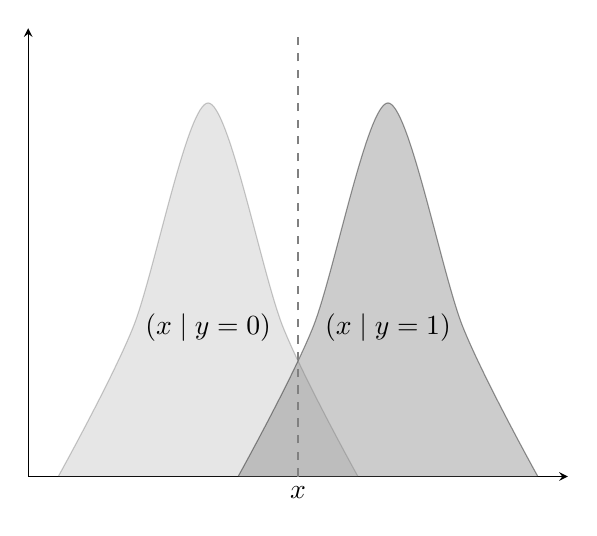
\begin{tikzpicture}
    \begin{axis}[
        ticks=none,
        axis x line=bottom,
        axis y line=left,
        xlabel={$x$},
        ymax=0.4,
        xmin=-2.2, xmax=1.4,
      ]
      % P(x|y=0)
      \addplot+[fill=gray, draw=black, opacity=0.2, smooth, mark=none] coordinates {
        (-2, 0.1) (-1.5, 0.2) (-1, 0.35) (-0.5, 0.2) (0, 0.1)
      };
      \node at (axis cs:-1, 0.2) {$\Prob(x \mid y = 0)$};
      % P(x|y=1)
      \addplot+[fill=gray, draw=black, opacity=0.4, smooth, mark=none] coordinates {
        (-0.8, 0.1) (-0.3, 0.2) (0.2, 0.35) (0.7, 0.2) (1.2, 0.1)
      };
      \node at (axis cs:0.2, 0.2) {$\Prob(x \mid y = 1)$};
      % Bayes
      \draw[dashed, gray] (axis cs:-0.4, 0) -- (axis cs:-0.4, 0.4);
    \end{axis}
  \end{tikzpicture}
  \tcblower
  The Bayes classifier is the line that separates the two classes.  The Bayes error is a
  result of the darker area in which the distributions of the classes intersect.
\end{figurebox}

\Cref{fig:bayes-classifier} illustrates the Bayes classifier and its error rate.
The vertical line represents the Bayes classifier that separates the classes the best way
possible in the space of the feature vectors $x$.  Since the distributions $\Prob(x \mid y
= 0)$ and $\Prob(x \mid y = 1)$ may intersect, there is a region where the Bayes
classifier cannot always predict the class correctly.

\subsection{Regression function}
\label{sec:regression-function}

In the regression estimation task, the goal is to approximate the optimal solution, called
\emph{regression function},
\begin{equation}
  \label{eq:regression-function}
  r(x) = \int y\, d\!\Prob(y \mid x)\text{,}
\end{equation}
that is the expected value of the target variable $y$ given the input $x$.

It is easy to show that the regression function minimizes the risk \eqref{eq:risk} with
loss
\[
  \mathcal{L}(y, r(x)) = \big(y - r(x)\big)^2\text{.}
\]
The risk functional for an arbitrary function $f$ is
\begin{multline*}
  R(f) =
    \int \big(y - f(x)\big)^2\, d\!\Prob(x, y) =\\
    \int y^2\, d\!\Prob(y) -
    2 \int f(x) \left[ \int y\, d\!\Prob(y \mid x) \right] d\!\Prob(x) +
    \int f(x)^2\, d\!\Prob(x)\text{,}
\end{multline*}
however we can substitute $r(x)$ for the inner integral and obtain
\begin{multline*}
  R(f) =
    \int y^2\, d\!\Prob(y) - 2 \int f(x) r(x)\, d\!\Prob(x) + \int f(x)^2\, d\!\Prob(x) = \\
    \int y^2\, d\!\Prob(y) + \int \left[ f(x)^2 - 2 f(x) r(x) \right]\, d\!\Prob(x)\text{.}
\end{multline*}
Once the first term is a constant, the risk is minimized by minimizing
\[
  f(x)^2 - 2 f(x) r(x)\text{.}
\]

Deriving the last expression with respect to $f(x)$ and setting it to zero, we obtain
\begin{equation*}
  \frac{d}{d f(x)} \Big[ f(x)^2 - 2 f(x) r(x) \Big] = 2 f(x) - 2 r(x) = 0 \Rightarrow
  f(x) = r(x)\text{.}
\end{equation*}

Like the Bayes classifier, the stochastic nature of the data leads to an irreducible
error in the regression estimation task.  We have that
\begin{equation*}
  R(r) = \int \big(y - r(x)\big)^2\, d\!\Prob(x, y) =
    \int y^2\, d\!\Prob(y) - \int r(x)^2\, d\!\Prob(x)\text{,}
\end{equation*}
where the first term is
\[
  \E\!\left[y^2\right] = \Var(y) + \E\!\left[y\right]^2
\]
and the second term is
\[
  \E\left[\E\!\left[y \mid x\right]^2\right] =
    \Var\!\left(\E\!\left[y \mid x\right]\right) + \E\!\left[\E\!\left[y \mid x\right]\right]^2 =
    \Var\!\left(\E\!\left[y \mid x\right]\right) + \E\!\left[y\right]^2\text{.}
\]
Thus, the irreducible error is
\[
  R(r) = \Var(y) - \Var\!\left(\E\!\left[y \mid x\right]\right) \text{.}
\]

The interpretation of the irreducible error comes from the law of the total variance:
\begin{equation*}
  \Var(y) = \E\!\left[ \Var(y \mid x) \right] + \Var\!\left(\E\!\left[y \mid x\right]\right)\text{,}
\end{equation*}
where the first term is known as the unexplained variance and the second term, as the
explained variance.  The equality $R(r) = \E\!\left[ \Var(y \mid x) \right]$
captures the idea that this variance is the intrinsic uncertainty that cannot be further
reduced.

\begin{figurebox}[label=fig:explained-unexplained-variance]{Unexplained variance is the
  error of the regression.}
  \centering
  \begin{tikzpicture}
    \begin{axis}[
        axis lines=middle,
        xlabel={$x$},
        ylabel={$y$},
        xmin=-0.2, xmax=1.5,
        ymin=-0.5, ymax=1.8,
        xtick={0, 0.5, 1},
        ytick={0, 0.5, 1},
        domain=0:1]

      \addplot[thick] {x} node[right] {$r(x) = x$};

      \addplot [draw=none, fill=gray, opacity=0.2] {x + 1} \closedcycle;
      \addplot [draw=none, fill=gray, opacity=0.2] {x - 1} \closedcycle;
      \draw[Stealth-Stealth, gray] (axis cs:0.5,0.5) -- (axis cs:0.5, 1.5) node[midway, right] {$\sigma = 1$};
      \node at (axis cs:0.5,1.3) [anchor=west] {Unexplained variance};

     \addplot[samples=2, style={dashed}] {0.5} node[midway, below, anchor=north west] {Explained variance};
    \end{axis}
  \end{tikzpicture}
  \tcblower
  Expected error of the regression function for data generated by
  $\Prob(y \mid x) \Prob(x)$ such that $\Prob(y \mid x) = \mathcal{N}(x, 1)$ and
  $\Prob(x) = \mathcal{U}(0, 1)$.  The regression function is $r(x) = x$.
\end{figurebox}

\Cref{fig:explained-unexplained-variance} illustrates the irreducible error of the
regression function for arbitrary distributions $\Prob(y \mid x)$ and $\Prob(x)$.
In this case, $\E\!\left[ \Var(y \mid x) \right] = 1$, which means that points drawn
by $\Prob(x, y)$ are distributed around the regression function $r(x)$ with a standard
deviation of one.  The explained variance is the spread of the regression across the
x-domain.

\section{ERM inductive principle}

It is very interesting to study the optimal solution for learning tasks, but in the
real-world, we do not have access to the distributions $\Prob(x)$ and $\Prob(y \mid x)$.
We must rely on the training data $(x_1, y_1), \dots, (x_n, y_n)$ to infer a solution.

In the following sections, for the sake of simplicity, let $z$ describe the pair $(x, y)$
and $L(z, \theta)$ be a generic loss function for the model $f_\theta$.  Note that the
training dataset is thus a set of $n$ i.i.d. samples $z_1, \dots, z_n$.

Since the distribution $\Prob(z)$ is unknown, the risk functional $R(\theta)$ is replaced by
the \emph{empirical risk functional}
\begin{equation}
  \label{eq:empirical-risk}
  R_n(\theta) = \frac{1}{n} \sum_{i=1}^n L(z_i, \theta)\text{.}
\end{equation}
```

Approximating $R(\theta)$ by the empirical risk functional $R_n(\theta)$ is the so-called
\gls{erm} inductive principle.  The ERM principle is the basis of the \gls{slt}.

Traditional methods, such as least squares, maximum likelihood, and maximum a posteriori, are
all realizations of the ERM principle for specific loss functions and hypothesis spaces.

\subsection{Consistency of the learning process}

One important question about the ERM principle is the consistency of the learning process.
Consistency means that, given a sufficient number of samples, the empirical risk
functional $R_n(\theta)$ converges to the true risk functional $R(\theta)$ over the
hypothesis space $\Theta$.

The consistency of the ERM principle is guaranteed by the uniform (two-sided)
convergence\footnote{Actually, only a weaker one-sided uniform convergence is needed; consult a
detailed explanation in chapter 2 of \fullcite{Vapnik1999b}.  The equivalence is a
consequence of the key theorem of learning proved by Vapnik and Chervonenkis in 1989 and
later translated to English in \fullcite{Vapnik1991}.} of the empirical risk functional
$R_n(\theta)$ to the true risk functional $R(\theta)$ over the hypothesis space $\Theta$.
The uniform convergence is defined as
\[
  \lim_{n \to \infty} \Prob\!\left(
    \sup_{\theta \in \Theta} \Big| R_n(\theta) - R(\theta) \Big| > \epsilon
  \right) = 0\text{.}
\]

\subsection{Rate of convergence}

Beyond consistency, it is also useful to understand the rate at which $R_n(\theta)$
converges to $R(\theta)$ as the sample size $n$ increases.  It is possible for a learning
machine to be consistent but have a slow convergence rate, which means that a large number of
samples is needed to achieve a good solution.

The asymptotic rate of convergence of the empirical risk functional $R_n(\theta)$ is
fast if, for any $n > n_0$, the exponential bound
\[
  \Prob\!\big(R(\theta_n) - R(\theta) > \epsilon\big) < \exp\!\left( - c n \epsilon^2 \right)
\]
holds true, where $c$ is a positive constant.

\subsection{VC entropy}

Let $L(z, \theta)$, $\theta \in \Theta$, be a set of bounded loss functions, i.e.
\[
  \left| L(z, \theta) \right| < M\text{,}
\]
for some constant $M$ and all $z$ and $\theta$.  One can construct $n$-dimensional vectors
\[
  l(z_1, \dots, z_n; \theta) = \big[ L(z_1, \theta), \dots, L(z_n, \theta) \big]\text{.}
\]
Once the loss functions are bounded, this set of vectors belongs to a $n$-dimensional
cube and has a finite minimal $\epsilon$-net\footnote{An $\epsilon$-net is a set of points
that are $\epsilon$-close to any point in the set.}.

Consider the quantity $N(z_1, \dots, z_n; \Theta, \epsilon)$ that counts the number of
elements of the minimal $\epsilon$-net of that set of vectors.
Once the quantity $N$ is a random variable, we can define the VC entropy as
\[
  H(n; \Theta, \epsilon) = \E\!\left[ \ln N(z_1, \dots, z_n; \Theta, \epsilon) \right]\text{,}
\]
where $z_i$ are i.i.d. samples drawn from some $\Prob(z)$.

If $L(z, \theta)$, $\theta \in \Theta$, is a set of indicator functions (i.e., the loss in a binary
classification task),  we measure the diversity of this set using the quantity $N(z_1,
\dots, z_n; \Theta)$ that counts the number of different separations of the given sample
that can be made by the functions.  In this case, the minimal $\epsilon$-net for $\epsilon < 1$
does not depend on $\epsilon$ and is a subset of the vertices of the unit cube.

A necessary and sufficient condition for uniform convergence is
\begin{equation}
  \label{eq:uniform-convergence}
  \lim_{n \to \infty} \frac{H(n; \Theta, \epsilon)}{n} = 0\text{,}
\end{equation}
for all $\epsilon > 0$.

The VC entropy measures the complexity of the hypothesis space $\Theta$.  The intuition
behind the need for a decreasing VC entropy with increasing numbers of observations is
related to the nonfalsifiability of the learning machine.  For instance, the set of
functions that can always separate the training data perfectly (contains all the vertices
of the cube) is nonfalsifiable because
it implies that the minimum of the empirical risk is zero independently of the value of
the true risk.

\subsection{Growing function and VC dimension}
\label{sub:vc-dimension}

It turns out that we can guarantee both the uniform convergence and the fast rate of
convergence independently of $\Prob(z)$.  Actually,
\[
  \lim_{n \to \infty} \frac{G(n; \Theta)}{n} = 0
\]
is the necessary and sufficient condition, where
\[
  G(n; \Theta) = \ln \sup_{z_1, \dots, z_n} N(z_1, \dots, z_n; \Theta)\text{,}
\]
is the \emph{growth function} of the hypothesis space $\Theta$.

\textcite{Vapnik1968}\footfullcite{Vapnik1968} showed that the growth function either
satisfies
\[
  G(n; \Theta) = n \ln 2
\]
or is bounded by
\[
  G(n; \Theta) \leq h \left( \ln \frac{n}{h} + 1 \right)\text{,}
\]
where $h$ is an integer.  Thus, the growth function is either linear or logarithmic in
$n$.  In the first case, we say that the \emph{VC dimension} of the hypothesis space is
infinite, and in the second case, the VC dimension is $h$.

A finite VC dimension is enough to imply both consistency and a fast rate of convergence.

\subsubsection{Intuitions about the VC dimension}
\label{sub:vc-dimension-intuition}

% A figure with lines separating separating points in a plane
\begin{figurebox}[label=fig:vc-dimension]{VC dimension of a set of lines in the plane.}
  \centering
  \begin{tikzpicture}
    \begin{axis}[
        axis lines=middle,
        xmin=-1, xmax=1,
        ymin=-1, ymax=1,
        xtick={0},
        ytick={0},
        domain=-1:1]

      \addplot[only marks, mark=*, mark size=2pt] coordinates {
        (-0.5, 0.3) (-0.3, -0.5) (0.7, -0.5)
      };

      % diagonal lines separating points
      \addplot[dashed] {x} node[right] {$\theta_1$};
      \addplot[dashed] {-x} node[right] {$\theta_2$};
      \addplot[dashed] {-0.3} node[right] {$\theta_3$};

    \end{axis}
  \end{tikzpicture}
  \tcblower
  The VC dimension of the lines in the plane is equal to 3, since a line can shatter 3
  points in all 8 possible ways, but not four points.
\end{figurebox}

For a set of indicator functions, the VC dimension is the maximum number of vectors that
can be \emph{shattered} by the functions.  If, for any $n$, there is a set of $n$
vectors that can be shattered by the functions, the VC dimension is infinite.
We say that $h$ vectors can be shattered if they can be separated into two classes in all
$2^h$ possible ways.  \Cref{fig:vc-dimension} illustrates the VC dimension of a set of
lines in the plane.

\begin{figurebox}[label=fig:vc-sin]{High-frequency sine wave functions have an infinite VC dimension.}
  \centering
  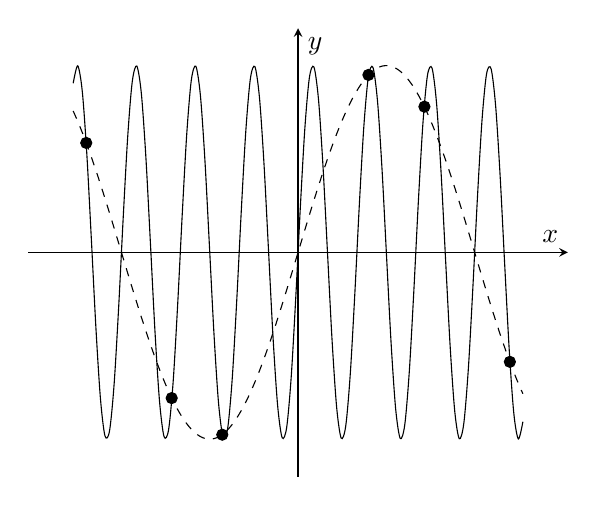
\begin{tikzpicture}
    \begin{axis}[
        axis lines=middle,
        xlabel={$x$},
        ylabel={$y$},
        xmin=-1.2, xmax=1.2,
        ymin=-1.2, ymax=1.2,
        xtick={0},
        ytick={0},
        domain=-1:1,
        samples=100]

      \addplot[smooth] {sin(deg(24 * x))};
      \addplot[dashed, smooth] {sin(deg(4 * x))};

      \addplot[only marks, mark=*, mark size=2pt] coordinates {
        (-0.942, 0.586) (-0.562, -0.780) (-0.337, -0.976)
        (0.313, 0.950) (0.562, 0.780) (0.942, -0.586)
      };
    \end{axis}
  \end{tikzpicture}
  \tcblower
  High-frequency sine waves approximate any set of points well, even though they may come
  from a low-frequency sine wave or any other function.
\end{figurebox}

One misconception about the VC dimension is that it is related to the number of parameters
of the model.  The VC dimension is actually related to the complexity of the hypothesis space, not
to the number of parameters.  For instance, the VC dimension of functions
\[
  f(z; \theta) = \mathbb{1}_{\sin \theta x > 0}
\]
is infinite, even though the parameter $\theta$ is a scalar.  See \cref{fig:vc-sin}.
By increasing the frequency $\theta$ of the sine wave, the function can approximate any set
of points.

This opens remarkable opportunities to find good solutions containing a huge number of
parameters\footnote{Sometimes, like in a linear model, the number of parameters is
proportional to the number of dimensions of the feature vector.} but with a finite VC
dimension.  % TODO: discuss non-parametric here?

\section{SRM inductive principle}

The \gls{erm} principle is a powerful tool to study the generalization ability of the
learning process.  By generalization ability, we mean the ability of the learning machine
to predict the output of new data that was not seen during the training process.  However,
it relies on the hypothesis that the number of samples tends to infinity.

In fact, \textcite{Vapnik1999b}\footfullcite{Vapnik1999b} summarizes the bounds for the
generalization ability of learning machines in the following way\footnote{ For the sake of
the arguments, we consider only the expression for bounded losses and an hypothesis space
with infinite number of functions.  Rigorously, the loss function may not be bounded;
consult the original work for the complete expressions.}:
\begin{equation}
  \label{eq:generalization-bound}
  R(\theta_n) \leq R_n(\theta_n) + \frac{B \mathcal{E}}{2} \left(
    1 + \sqrt{1 + \frac{4 R_n(\theta_n)}{B \mathcal{E}}}
  \right)\text{,}
\end{equation}
with
\[
  \mathcal{E} = 4 \frac{
    h \left( \ln \frac{2 n}{h} + 1 \right) - \ln \frac{\eta}{4}
  }{n}\text{,}
\]
where $B$ is the upper bound of the loss function, $h$ is the VC dimension of the
hypothesis space, $n$ is the number of samples.  The term $\eta$ is the confidence level,
i.e., the inequality holds with probability $1 - \eta$.

It is easy to see that as the number of samples $n$ increases, the empirical risk
$R_n(\theta_n)$ approaches the true risk $R(\theta_n)$.  Also, the greater the VC
dimension $h$, the greater the term $\mathcal{E}$, decreasing the generalization ability
of the learning machine.

In other words, if $\nicefrac{n}{h}$ is small, a small empirical risk does not guarantee a small value
for the actual risk.  A consequence is that we need to minimize both terms of the
right-hand side of the inequality \cref{eq:generalization-bound} to achieve a good
generalization ability.

% A table comparing overfit and underfit and the empirical risk and confidence interval
\begin{tablebox}[label=tab:overfit-underfit]{Overfitting and underfitting.}
  \centering
  \begin{tabular}{lll}
    \toprule
    \textbf{Problem} & \textbf{Empirical risk} & \textbf{Confidence interval} \\
    \midrule
    Underfitting & High & Low \\
    Overfitting & Low & High \\
    \bottomrule
  \end{tabular}
  \tcblower
  Two problems that can arise in the learning process are underfitting and overfitting.
  Underfitting occurs when the model is too simple (low VC dimension) and cannot capture
  the complexity of the training data (high empirical risk).  Overfitting occurs when the
  model is too complex (high VC dimension increases the confidence interval) and fits the
  training data almost perfectly (low empirical risk).
\end{tablebox}

Failure to balance the optimization of these terms leads to two problems: underfitting and
overfitting.  \Cref{tab:overfit-underfit} summarizes the problems.

The \gls{srm} principle consists of minimizing both the empirical risk (optimizing the
parameters of the model) and the confidence interval (controlling VC dimension).

Let $\Theta_k \subset \Theta$ and
\[
  S_k = \left\{ L(z, \theta) : \theta \in \Theta_k \right\}
\]
such that
\[
  S_1 \subset S_2 \subset \dots \subset S_n \subset \dots\text{,}
\]
satisfying
\[
  h_1 \leq h_2 \leq \dots \leq h_n \leq \dots\text{,}
\]
where $h_k$ is the finite VC dimension\footnote{Note that the VC dimension considering the
whole set $\Theta$ might be infinite.  Moreover, in the original formulation, the sets
$S_k$ also need to satisfy some bounds; read more in chapter 4 of \fullcite{Vapnik1999b}.}
of each set $S_k$.  This is called an \emph{admissible structure}.

\begin{figurebox}[label=fig:srm-tradeoff]{SRM trade-off.}
  \centering
  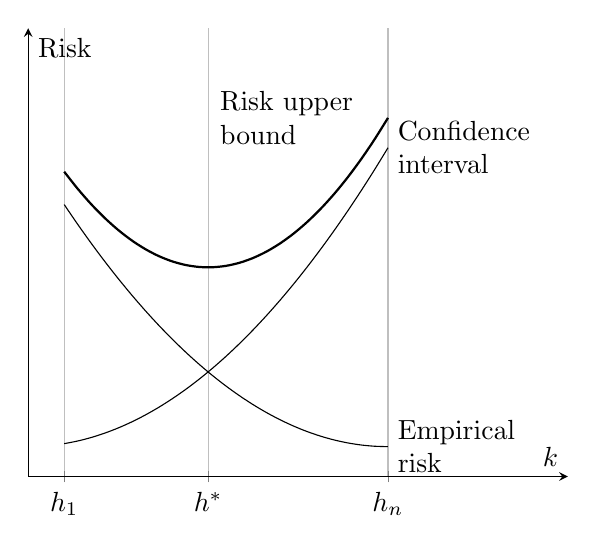
\begin{tikzpicture}
    \begin{axis}[
        axis lines=middle,
        xlabel={$k$},
        ylabel={Risk},
        ytick={0},
        yticklabels={},
        xtick={0.1, 0.5, 1},
        xticklabels={$h_1$, $h^*$, $h_n$},
        grid=both,
        xmin=0, xmax=1.5,
        ymin=0, ymax=1.5,
        domain=0.1:1]

      \addplot[smooth] {(x - 1)^2 + 0.1} node[right, text width=2cm] {Empirical risk};
      \addplot[smooth] {x^2 + 0.1} node[right, text width=2cm] {Confidence interval};
      \addplot[smooth, thick] {x^2 + (x - 1)^2 + 0.2} node[left, text width=2cm] {Risk upper bound};

    \end{axis}
  \end{tikzpicture}
  \tcblower
  The upper bound of the risk is the sum of the empirical risk and the confidence
  interval.  The smallest bound is found for some $k^*$ in the admissible structure.
\end{figurebox}

Given the observations $z_1, \dots, z_n$, the \gls{srm} principle chooses a function
$L(z, \theta_n^k)$ that minimizes the empirical risk $R_n(\theta_n^k)$ in the subset
$S_k$ for which the guaranteed risk --- upper bound considering the confidence interval
--- is minimal.  This is a trade-off between the quality of the approximation and the
complexity of the approximating function --- see \cref{fig:srm-tradeoff}.

\subsection{Bias invariance trade-off}

The trade-off that the \gls{srm} principle deals with is the general case of the so-called
\emph{bias-variance trade-off}.  The bias-variance trade-off is a well-known concept in
machine learning that describes the relationship between different kinds of errors a model
can have.

The \emph{bias error} comes from failure to capture relevant relationships between features
and target outputs.  The \emph{variance error} comes from erroneously modeling the random
noise in the training data.

The terms bias and variance (and the irreducible error) are clearly illustrated by
studying the particular regression estimation task.

Consider a learning machine that produces a function $\hat{f}(x; D)$ based on the
training set $$D = \big\{(x_1, y_1), \dots, (x_n, y_n)\big\}$$ such that
\[
  y_i = f(x_i) + \epsilon\text{,}
\]
for a fixed function $f$ and a random noise $\epsilon$ with zero mean and variance
$\sigma^2$, where $x_i$ are i.i.d. samples drawn from some distribution $\Prob(x)$.

Also, consider that $\bar{f}(x)$ is the expected value of the function $\hat{f}(x; D)$
over all possible training sets $D$, i.e.
\[
  \bar{f}(x) = \int \hat{f}(x; D)\, d\!\Prob(D)\text{.}
\]
(Note that the models themselves are the random variable we are studying here.)

For any model $\hat{f}$, the expected (squared) error for a particular sample $(x, y)$,
$\E_D\!\left[ \big( y - \hat{f}(x; D) \big)^2 \right]$, is
\begin{align}
  \notag \int \big( y - \hat{f}(x) \big)^2\, d\!\Prob(D, \epsilon)
    &= \int \big( y - f(x) + f(x) - \hat{f}(x) \big)^2\, d\!\Prob(D, \epsilon) \\
    &= \label{eq:term1}\int \big( y - f(x) \big)^2\, d\!\Prob(D) \\
    &+ \label{eq:term2}\int \big( f(x) - \hat{f}(x) \big)^2\, d\!\Prob(D) \\
    &+ \label{eq:term3}2 \int \big( y - f(x) \big)\,\big( f(x) - \hat{f}(x) \big)\, d\!\Prob(D, \epsilon)\text{.}
\end{align}

The term \eqref{eq:term1} is the irreducible error:
\begin{equation}
  \label{eq:irreducible-error}
  \int \big( y - f(x) \big)^2\, d\!\Prob(D) =
  \int \big( f(x) + \epsilon - f(x) \big)^2\, d\!\Prob(D) =
  \int \epsilon^2\, d\!\Prob(D) = \sigma^2\text{.}
\end{equation}
As the best solution is $f$ itself, the error that comes from the noise is unavoidable.

The term \eqref{eq:term3} is null:
\begin{multline*}
  \int \big( y - f(x) \big)\,\big( f(x) - \hat{f}(x) \big)\, d\!\Prob(D, \epsilon) =
  \int \epsilon\,\big( f(x) - \hat{f}(x) \big)\, d\!\Prob(D, \epsilon) = \\
  \cancelto{0}{\int \epsilon\, d\!\Prob(\epsilon)} \int \big( f(x) - \hat{f}(x) \big)\, d\!\Prob(D) = 0\text{,}
\end{multline*}
since $\Prob(D)$ and $\Prob(\epsilon)$ are independent and $\E[\epsilon] = 0$ by
definition.

We can apply a similar strategy to analyze the term \eqref{eq:term2}:
\begin{align}
  \notag \int \big( f(x) - \hat{f}(x) \big)^2\, d\!\Prob(D)
    &= \int \big( f(x) - \bar{f}(x) + \bar{f}(x) - \hat{f}(x) \big)^2\, d\!\Prob(D) \\
    &= \label{eq:term4}\int \big( f(x) - \bar{f}(x) \big)^2\, d\!\Prob(D) \\
    &+ \label{eq:term5}\int \big( \bar{f}(x) - \hat{f}(x) \big)^2\, d\!\Prob(D) \\
    &+ \label{eq:term6}2 \int \big( f(x) - \bar{f}(x) \big)\,\big( \bar{f}(x) - \hat{f}(x) \big)\, d\!\Prob(D)\text{.}
\end{align}

Now, the term \eqref{eq:term6} is also null:
\begin{multline*}
  \int \big( f(x) - \bar{f}(x) \big)\,\big( \bar{f}(x) - \hat{f}(x; D) \big)\, d\!\Prob(D) = \\
  \big( f(x) - \bar{f}(x) \big) \int \big( \bar{f}(x) - \hat{f}(x; D) \big)\, d\!\Prob(D) = \\
  \big( f(x) - \bar{f}(x) \big) \cancelto{0}{\left( \bar{f}(x) - \int \hat{f}(x; D)\, d\!\Prob(D) \right)} = 0\text{,}
\end{multline*}
since $\bar{f}(x)$ is the expected value of $\hat{f}(x; D)$.

The term \eqref{eq:term4} does not depend on the training set, so
\begin{equation}
  \label{eq:bias}
  \int \big( f(x) - \bar{f}(x) \big)^2\, d\!\Prob(D) =
  \big( f(x) - \bar{f}(x) \big)^2\text{.}
\end{equation}
This term is the square of the bias of the models.

The term \eqref{eq:term5} is the variance of the function $\hat{f}(x; D)$:
\begin{multline}
  \label{eq:model-variance}
  \int \big( \bar{f}(x) - \hat{f}(x; D) \big)^2\, d\!\Prob(D) =\\
  \E_D\!\left[ \big( \bar{f}(x) - \hat{f}(x; D) \big)^2 \right] =
  \Var_D\!\left( \hat{f}(x; D) \right)\text{.}
\end{multline}

Finally, putting all together --- i.e.  \cref{eq:irreducible-error,eq:bias,eq:model-variance}
---, we have that the expected error for a particular sample $(x, y)$ is
\[
  \E_D\!\left[ \big( y - \hat{f}(x; D) \big)^2 \right] =
    \sigma^2 +
    \big( f(x) - \E\!\left[ \hat{f}(x; D) \right] \big)^2 +
    \Var_D\!\left( \hat{f}(x; D) \right)\text{.}
\]

The irreducible error is the regression error that cannot be reduced by any model --- see
\cref{sec:regression-function}.  The bias error is the error that one expects from the
model acquired by the learning machine and that we observe in the training data --- i.e.
the empirical risk.  The variance error, which does not depend on the real function $f$
but on the models the learning machine can generate, is the error that comes from how
different the models can be from each other --- i.e. the confidence interval that comes from
the VC dimension.

\subsection{Regularization}

Also related to the \gls{srm} principle is the concept of \emph{regularization}.
Regularization encourages models to learn robust patterns within the data rather than
memorizing it.

Regularization techniques usually modify the loss by adding a penalty term that
depends on the complexity of the model.  So, instead of minimizing the empirical risk
$R_n(\theta)$, the learning machine minimizes the regularized empirical risk
\[
  R_n(\theta) + \lambda \Omega(\theta)\text{,}
\]
where $\Omega(\theta)$ is the complexity of the model and $\lambda$ is a hyperparameter
that controls the trade-off between the empirical risk and the complexity.
Note that the regularization term acts as a proxy for the confidence interval in the
\gls{srm} principle.  However, regularization is often justified by common sense or
intuition, rather than by strong theoretical arguments.

Other approaches that indirectly control the complexity of the model --- such as early
stopping, dropout, ensembles, and pruning --- are often called implicit regularization.

\section{Linear problems}

To realize the concepts of the \gls{srm} principle in practice, we consider linear
classification tasks.

For the examples in the following subsections, we use the datasets for the AND
and the XOR problem --- see \cref{tab:and-xor}.
The AND problem is linearly separable, while the XOR problem is not.

\begin{tablebox}[label=tab:and-xor]{AND and XOR datasets.}
  \centering
  \begin{minipage}{0.45\textwidth}
    \centering
    \rowcolors{2}{black!10!white}{}
    \begin{tabular}{ccc}
      \toprule
      $x_1$ & $x_2$ & $y = x_1 \land x_2$ \\
      \midrule
      0 & 0 & 0 \\
      0 & 1 & 0 \\
      1 & 0 & 0 \\
      1 & 1 & 1 \\
      \bottomrule
    \end{tabular}
  \end{minipage}
  \begin{minipage}{0.45\textwidth}
  \centering
  \rowcolors{2}{black!10!white}{}
  \begin{tabular}{ccc}
    \toprule
    $x_1$ & $x_2$ & $y = x_1 \oplus x_2$ \\
    \midrule
    0 & 0 & 0 \\
    0 & 1 & 1 \\
    1 & 0 & 1 \\
    1 & 1 & 0 \\
    \bottomrule
  \end{tabular}
  \end{minipage}
  \tcblower
  The AND and XOR datasets are binary classification datasets where the output $y$ is the
  ``logical AND'' and the ``exclusive OR'' of the inputs $x_1$ and $x_2$, i.e.,
  $y = x_1 \land x_2$ and $y = x_1 \oplus x_2$.
\end{tablebox}

We show two learning machines that implement the \gls{srm} principle in different ways:
\begin{itemize}
  \itemsep0em
  \item The perceptron, which fixes the complexity of the model and tries to minimize the
    empirical risk; and
  \item The maximal margin classifier, which fixes the empirical risk --- in this case,
    zero -- and tries to minimize the confidence interval.
\end{itemize}

\subsection{Perceptron}
\label{sub:perceptron}

The perceptron is a linear classifier that generates a hyperplane that separates the
classes in the feature space.  It is a parametric model, and the learning process minimizes the empirical risk
by adjusting its fixed set of parameters.

\begin{defbox}{Parametric model}{parametric}
  If the learning machine generates a set of functions $f_\theta$ where the number of
  parameters $|\theta|$ is always fixed, the models are called \emph{parametric}.
\end{defbox}

Parametric models are usually simpler and faster to fit, but they are less flexible.  In
other words, it is up to the researcher to choose the best model ``size'' for the problem.
If the model is too small, it will not be able to capture the complexity of the data.  If
the model is too large, it tends to be too complex, too slow to train, and might overfit to
the data.  Note, however, that the VC dimension and number of parameters are not the same
thing --- consult \cref{sub:vc-dimension-intuition}.

The perceptron model (with two inputs) is
\begin{equation*}
  f(x_1, x_2; \vec{w} = \left[w_0, w_1, w_2\right]) = u(w_0 + w_1 x_1 + w_2 x_2)\text{,}
\end{equation*}
where $u$ is the Heaviside step function
\begin{equation*}
  u(x) = \begin{cases}
    1 & \text{if } x > 0\text{,} \\
    0 & \text{otherwise.}
  \end{cases}
\end{equation*}
The parameters $\theta = \vec{w}$ are called the weights of the perceptron.
The equation $\vec{w} \cdot \vec{x} = 0$, where $\vec{x} = [1, x_1,
x_2]$, is the equation of a hyperplane.

\begin{figurebox}[label=fig:perceptron-and]{Perceptron decision boundaries in the AND dataset.}
  \centering
  \begin{tikzpicture}
    \begin{axis}[
        axis x line=bottom,
        axis y line=left,
        xlabel={$x_1$},
        ylabel={$x_2$},
        width=0.6\textwidth,
        height=0.6\textwidth,
        xtick={0, 1},
        ytick={0, 1},
        xmin=-0.5, xmax=1.5,
        ymin=-0.5, ymax=1.5,
      ]
      \addplot+[only marks, mark=-, color=black, mark size=3pt] coordinates {
        (0, 0) (0, 1) (1, 0)
      };
      \addplot+[only marks, mark=+, color=black, mark size=3pt] coordinates {
        (1, 1)
      };
      \addplot+[domain=0:1.5, mark=none, black, thick] {1.1 - 0.6 * x};
    \end{axis}
  \end{tikzpicture}
  \tcblower
  The perceptron assumes that the classes are linearly separable.
  The hyperplane that separates the classes comes from the weights of the model.
  In this case, $w_0 = -1.1$, $w_1 = 0.6$, and $w_2 = 1$.
\end{figurebox}

In \cref{fig:perceptron-and}, we show the hyperplane (in this case, a line) that the model
with weights $\vec{w} = [-1.1, 0.6, 1]$ generates in this feature space.
As one can see, the classes are linearly separable, and the perceptron model classifies
the dataset correctly; see \cref{tab:and-perceptron}.

\begin{tablebox}[label=tab:and-perceptron]{Truth table for the predictions of the perceptron in the AND dataset.}
  \centering
  \rowcolors{2}{black!10!white}{}
  \begin{tabular}{ccc|cc}
    \toprule
    $x_1$ & $x_2$ & $y$ & $-1.1 + x_1 + x_2$ & $\hat{y}$ \\
    \midrule
    0 & 0 & 0 & -1.1 & 0 \\
    0 & 1 & 0 & -0.1 & 0 \\
    1 & 0 & 0 & -0.5 & 0 \\
    1 & 1 & 1 & 0.5 & 1 \\
    \bottomrule
  \end{tabular}
  \tcblower
  The perceptron model with parameters $w_0 = 1.1$, $w_1 = -1$, and $w_2 = -1$
  classifies the AND dataset correctly.
\end{tablebox}

\begin{figurebox}[label=fig:perceptron-xor]{Perceptron decision boundaries in the XOR
  dataset.}
  \centering
  \begin{tikzpicture}
    \begin{axis}[
        axis x line=bottom,
        axis y line=left,
        xlabel={$x_1$},
        ylabel={$x_2$},
        width=0.6\textwidth,
        height=0.6\textwidth,
        xtick={0, 1},
        ytick={0, 1},
        xmin=-0.5, xmax=1.5,
        ymin=-0.5, ymax=1.5,
      ]
      \addplot+[only marks, mark=-, color=black, mark size=3pt] coordinates {
        (0, 0) (1, 1)
      };
      \addplot+[only marks, mark=+, color=black, mark size=3pt] coordinates {
        (0, 1) (1, 0)
      };
      \addplot+[domain=0:1.5, mark=none, black, thick] {-0.5 + x};
    \end{axis}
  \end{tikzpicture}
  \tcblower
  The XOR dataset is not linearly separable.
  The hyperplane that separates the classes comes from the weights of the model.
  In this case, $w_0 = -0.5$, $w_1 = 1$, and $w_2 = -1$.
  There is no way to classify the XOR dataset correctly with a perceptron.
\end{figurebox}

In \cref{fig:perceptron-xor}, we show the hyperplane that the model $\vec{w} = [-0.5, 1, -1]$
generates for the XOR dataset.  As one can see, the perceptron model fails to solve the
task since there is no single decision boundary that can classify this data.

\begin{tablebox}[label=tab:xor-perceptron]{Truth table for the predictions of the perceptron in the XOR dataset.}
  \centering
  \rowcolors{2}{black!10!white}{}
  \begin{tabular}{ccc|cc}
    \toprule
    $x_1$ & $x_2$ & $y$ & $-0.5 + x_1 - x_2$ & $\hat{y}$ \\
    \midrule
    0 & 0 & 0 & -0.5 & 0 \\
    0 & 1 & 1 & -1.5 & 0 \\
    1 & 0 & 1 & 0.5 & 1 \\
    1 & 1 & 0 & -0.5 & 0 \\
    \bottomrule
  \end{tabular}
  \tcblower
  The perceptron model with parameters $w_0 = -0.5$, $w_1 = 1$, and $w_2 = -1$
  fails to classify the XOR dataset correctly --- as any other perceptron would do.
\end{tablebox}

It is easy to see that there are an infinite number of hyperplanes that can separate the
classes in the AND dataset.  The training procedure of the perceptron is a simple
algorithm that adjusts the weights of the model to find one of these hyperplanes ---
effectively minimizing the empirical risk.  The algorithm updates the weights iteratively
for each sample that is misclassified, repeating the samples as many times as necessary.
It stops when all samples are correctly classified.

For a binary classification problem and a perceptron with weights $\vec{w}$, there are 4
situations for a given sample $\vec{x}$ and $y$:
\begin{enumerate}
  \itemsep0em
  \item $y = 0$ and $u(\vec{w} \cdot \vec{x})= 0$;
  \item $y = 0$ and $u(\vec{w} \cdot \vec{x})= 1$;
  \item $y = 1$ and $u(\vec{w} \cdot \vec{x})= 0$;
  \item $y = 1$ and $u(\vec{w} \cdot \vec{x})= 1$.
\end{enumerate}

By definition, the algorithm must update the weights when situation 2 or 3 occurs.
Let $e = y - u(\vec{w} \cdot \vec{x})$ be the error of the model for a given sample.

In situation 2, we have that $\vec{w} \cdot \vec{x} > 0$ which means that the angle
$\alpha$ between the vectors $\vec{w}$ and $\vec{x}$ is less than $90^\circ$, since
$\|\vec{w}\|\|\vec{x}\|\cos\alpha > 0 \implies \cos\alpha > 0 \implies \alpha <
90^\circ$.  To increase the angle between the vectors, we can subtract $\eta\vec{x}$ from
$\vec{w}$, for some small $\eta > 0$ --- see \cref{fig:perceptron-w2}.  The error
here is $e = -1$.

\begin{figurebox}[label=fig:perceptron-w2]{Angle between $\vec{w}$ and $\vec{x}$ in a positive output.}
  \centering
  \begin{tikzpicture}
    \draw[-Stealth] (0, 0) -- (2, 0) node[right] {$\vec{x}$};
    \draw[-Stealth] (0, 0) -- (1, 1.8) node[right] {$\vec{w}$};
    \draw[-Stealth, dashed] (1, 1.8) -- (-0.4, 1.8) node[above] {$-\eta\vec{x}$};
    \draw[-Stealth, thick, gray] (0, 0) -- (-0.4, 1.8) node[left] {$\vec{w}'$};
    \draw (0.4, 0) arc (0:59:0.4) node[right] {$\alpha$};
  \end{tikzpicture}
  \tcblower
  A positive output for the perceptron with weights $\vec{w}$ and input $\vec{x}$ means
  that the angle between the vectors is less than $90^\circ$.  To increase the angle
  between the vectors, we can subtract $\eta\vec{x}$ from $\vec{w}$, for some small $\eta
  > 0$.
\end{figurebox}

In situation 3, we have that $\vec{w} \cdot \vec{x} < 0$ which means that the
angle $\alpha$ between the vectors $\vec{w}$ and $\vec{x}$ is greater than $90^\circ$,
since $\|\vec{w}\|\|\vec{x}\|\cos\alpha < 0 \implies \cos\alpha < 0 \implies \alpha > 90^\circ$.
To decrease the angle between the vectors, we can add $\eta\vec{x}$ to $\vec{w}$, for
some small $\eta > 0$ --- see \cref{fig:perceptron-w3}.  Now, the error is $e = 1$.

\begin{figurebox}[label=fig:perceptron-w3]{Angle between $\vec{w}$ and $\vec{x}$ in a negative output.}
  \centering
  \begin{tikzpicture}
    \draw[-Stealth] (0, 0) -- (2, 0) node[right] {$\vec{x}$};
    \draw[-Stealth, thick, gray] (0, 0) -- (1, 1.8) node[right] {$\vec{w}'$};
    \draw[-Stealth, dashed] (-0.4, 1.8) -- (1, 1.8) node[above] {$\eta\vec{x}$};
    \draw[-Stealth] (0, 0) -- (-0.4, 1.8) node[left] {$\vec{w}$};
    \draw (0.4, 0) arc (0:101:0.4) node[above] {\phantom{a }$\alpha$};
  \end{tikzpicture}
  \tcblower
  A negative output for the perceptron with weights $\vec{w}$ and input $\vec{x}$ means
  that the angle between the vectors is greater than $90^\circ$.  To decrease the angle
  between the vectors, we can add $\eta\vec{x}$ to $\vec{w}$, for some small $\eta
  > 0$.
\end{figurebox}

From those observations, we can derive a general update rule
\[
  \vec{w}' = \vec{w} + \eta e \vec{x}\text{,}
\]
where $\eta$ is a small positive number that controls the step size of the algorithm.
Note that this rule works even for cases 1 and 4, where the error is zero.

The algorithm converges given $\eta$ sufficiently small and the dataset is linearly
separable.  Note that the algorithm does not make any effort to reduce the confidence
interval.

The perceptron is (possibly) the simplest artificial neural network.  More complex
networks can be built by stacking perceptrons in layers and adding non-linear activation
functions.  The training strategies for those networks are usually based on reducing the
empirical risk using the gradient descent algorithm while controlling the complexity of
the model with regularization techniques\footnote{To counterbalance the potential
``excess'' of neurons, techniques like $l_2$ regularization ``disable'' some neurons by
pressuring their weights to zero.}.  Consult \cref{sec:mlp}.

% TODO: adaline for regression

\subsection{Maximal margin classifier}

We saw that the perceptron tries to minimize the empirical risk, but it makes no effort to
reduce the confidence interval.  A different approach would be to fix the empirical risk
--- in our case, assuming that the classes are linearly separable, to fix it to zero --- and
minimize the confidence interval.

The confidence interval is an increasing function
\[
  \Omega\!\left(\frac{h}{n}\right)\text{,}
\]
where $h$ is the VC dimension of the hypothesis space and $n$ is the number of samples.
Since the number of training samples $n$ is fixed and finite (sometimes even small), we
can minimize the confidence interval by minimizing the VC dimension $h$.

In the case of the perceptron, since it can generate any hyperplane, the VC dimension is
$h = d + 1$, where $d$ is the number of dimensions of the feature space --- consult
\cref{sub:vc-dimension-intuition}.

Before we dive into the classifier that minimizes the confidence interval, consider the
following property.  \textcite{Vapnik1999b}\footfullcite{Vapnik1999b} state that a
$\Delta$-margin separating hyperplane is the hyperplane
\[
  (\vec{w} \cdot \vec{x}) - b = 0\text{, } \|\vec{w}\| = 1\text{,}
\]
such that classifies vector $\vec{x}$ as
\[
  y = \begin{cases}
    1 & \text{if } (\vec{w} \cdot \vec{x}) - b \geq \Delta\text{,} \\
    -1 & \text{if } (\vec{w} \cdot \vec{x}) - b \leq -\Delta\text{.}
  \end{cases}
\]
Given that vectors $\vec{x} \in \mathbb{R}^d$ belong to a (hyper)sphere of radius $R$, the
VC dimension of the $\Delta$-margin separating hyperplane is
\[
  h \leq \min\left(\left\lfloor \frac{R^2}{\Delta^2} \right\rfloor, d\right) + 1\text{,}
\]
which can be less than $d + 1$.

From that property, to minimize the confidence interval, we can maximize the margin
$\Delta$ of the hyperplane.  The \emph{maximal margin classifier} is a learning machine
that generates the hyperplane that separates the classes with no error and maximizes the
margin between the classes.

\begin{figurebox}[label=fig:maximal-margin-and]{Maximal margin classifier for the AND dataset.}
  \centering
  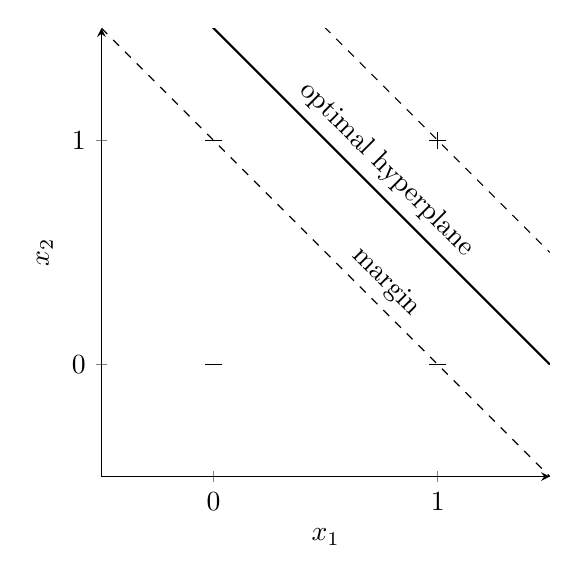
\begin{tikzpicture}
    \begin{axis}[
        axis x line=bottom,
        axis y line=left,
        xlabel={$x_1$},
        ylabel={$x_2$},
        width=0.6\textwidth,
        height=0.6\textwidth,
        xtick={0, 1},
        ytick={0, 1},
        xmin=-0.5, xmax=1.5,
        ymin=-0.5, ymax=1.5,
        domain=-0.5:1.5,
      ]
      \addplot+[only marks, mark=-, color=black, mark size=3pt] coordinates {
        (0, 0) (0, 1) (1, 0)
      };
      \addplot+[only marks, mark=+, color=black, mark size=3pt] coordinates {
        (1, 1)
      };
      \addplot+[mark=none, black, thick] {1.5 - x} node[above, pos=0.6, rotate=-45] {optimal hyperplane};
      \addplot+[mark=none, black, dashed] {1 - x} node[above, pos=0.6, rotate=-45] {margin};
      \addplot+[mark=none, black, dashed] {2 - x};
    \end{axis}
  \end{tikzpicture}
  \tcblower
  The maximal margin classifier generates the hyperplane that maximizes the margin between
  the classes.  In this case, the margin is $\Delta = 0.5$.
\end{figurebox}

Thus, given the training set $(\vec{x}_1, y_1), \dots, (\vec{x}_n, y_n)$, $\vec{x} \in
\mathbb{R}^d$ and $y_i \in \{-1, 1\}$, the optimal hyperplane --- see
\cref{fig:maximal-margin-and} --- is the one that satisfies
\[
  y_i \left[(\vec{w} \cdot \vec{x}_i - b)\right] \geq 1\text{,}
\]
for all $i = 1, \dots, n$ that minimizes $\|\vec{w}\|^2$.  The intuition of the
minimization of the coefficients is that we want only the vectors in the margin to be
exactly equal to $\pm 1$.  (Consequently, the vectors farther from the margin have values
greater than $1$ or less than $-1$.)

Without entering into the details of the optimization process, one interesting property of
the maximal margin classifier is that the separating hyperplane is built from the \emph{support vectors}
--- the vectors that are exactly in the margin.  In \cref{fig:maximal-margin-and}, the
support vectors are the points $(1, 0)$, $(0, 1)$, and $(1, 1)$.

In other words, maximal margin classifier is
\[
  f(x) = \sign\left(\sum_{i=1}^{n} y_i a_i \big(\vec{x}_i \cdot x\big) - b\right)\text{,}
\]
for some $b$ and coefficients $a_i > 0$ for the support vectors ($a_i = 0$ otherwise).

In the case that the classes are not linearly separable, the maximal margin classifier can
be extended to the \emph{soft margin classifier}, which sets the empirical risk to a value
greater than zero.

Moreover, since the number of parameters of the maximal margin classifier depends on the
training data (i.e., the number of support vectors), it is a nonparametric model.
Nonparametric models are those in which the number of parameters is not fixed and can grow
as needed to fit the data.  This property becomes more clear when we consider the kernel
trick, which allows the maximal margin classifier to deal with nonlinear problems.
Consult \textcite{Vapnik1999b}\footfullcite{Vapnik1999b} for more details.

\section{Closing remarks}

% TODO: more parameters do not mean higher VC dimension. We measure the complexity of the
% learning process, not the model itself.

The \gls{srm} principle is a powerful tool to understand the generalization ability of
learning machines.  The principle not only explains many of the empirical results in
\gls{ml} but also provides a theoretical framework to guide the development of new
learning machines.

Many powerful methods have been proposed in the literature --- e.g., support vector
machines, boosting, and deep learning --- that can deal with complex nonlinear problems.
I encourage the reader to dive into the literature to learn more about these methods and
the theoretical principles behind them.  Some comments about a few methods are given in
\cref{chap:learning-machines}.

% vim: spell spelllang=en

\chapter{Data preprocessing}
\label{chap:preprocess}
\glsresetall

\chapterprecishere{I find your lack of faith disturbing.
  \par\raggedleft--- \textup{Darth Vader}, Star Wars: Episode IV -- A New Hope (1977)}

In this chapter, we discuss the data preprocessing, which is the process of adjusting the
data to make it suitable for a particular learning machine or, at the least, to ease the
learning process.

Similarly to data handling, data preprocessing is done by applying a series of operations
to the data.  However, some of the parameters of the operations are not fixed but rather
are fit from a data sampling.  In the context of inductive learning, the sampling is the
training set.

The operations are dependent on the chosen learning method.  So, when planning the
solution in our project, we must consider the preprocessing tasks that are necessary to
make the data suitable for the chosen methods.

I present the most common data preprocessing tasks in three categories: data cleaning,
data sampling, and data transformation.  For each task, I discuss the behavior of the data
preprocessing techniques in terms of fitting, adjustment of the training set, and
application of the preprocessor in production.

Finally, I discuss the importance of the default behavior of the model when the
preprocessing chain degenerates over a sample, i.e. when the preprocessor decides that it
has no strategy to adjust the data to make it suitable for the model.

\begin{mainbox}{Chapter remarks}

  \boxsubtitle{Contents}

  \startcontents[chapters]
  \printcontents[chapters]{}{1}{}
  \vspace{1em}

  \boxsubtitle{Context}

  \begin{itemize}
    \itemsep0em
    \item Tidy data is not necessarily suitable for modeling.
    \item Parameters of the preprocessor are fitted rather than being fixed.
  \end{itemize}

  \boxsubtitle{Objectives}

  \begin{itemize}
    \itemsep0em
    \item Understand the main data preprocessing tasks and techniques.
    \item Learn the behavior of the preprocessing chain in terms of fitting, adjustment,
      and application.
  \end{itemize}

  \boxsubtitle{Takeaways}

  \begin{itemize}
    \itemsep0em
    \item Each learning method requires specific data preprocessing tasks.
    \item Fitting the preprocessor is crucial to avoid leakage.
    \item Default behavior of the model when the preprocessing chain degenerates must be
      specified.
  \end{itemize}
\end{mainbox}

{}
\clearpage

\section{Introduction}

In \cref{chap:data,chap:handling}, we discussed data semantics and the tools to
handle data.  They provide the grounds for preparation of the data as we described in the
data sprint tasks in \cref{sub:workflow}.  However, the focus is to guarantee that the
data is tidy and in the observational unit of interest, not to prepare it for modeling.

As a result, although data might be appropriate for the learning tasks we described in
\cref{chap:slt} --- in the sense that we know what the feature vectors and the target
variable are ---, they might not be suitable for the machine learning methods we will use.

One simple example is the perceptron (\cref{sub:perceptron}) that assumes all
input variables are real numbers.  If the data contains categorical variables, we must
convert them to numerical variables before applying the perceptron.

For this reason, the solution sprint tasks in \cref{sub:workflow} include not only the
learning tasks but also the \emph{data preprocessing} tasks, which are dependent on the
chosen machine learning methods.

\begin{defbox}{Data preprocessing}{preprocessing}
  The process of adjusting the data to make it suitable for a particular learning machine
  or, at the least, to ease the learning process.
\end{defbox}

This is done by applying a series of operations to the data, like in data handling.  The
difference here is that some of the parameters of the operations are not fixed; rather, they
are fit from a data sampling.  Once fitted, the operations can be applied to
new data, sample by sample.

As a result, a data processing technique acts in three steps:
\begin{enumerate}
  \itemsep0em
  \item \textbf{Fitting}: The parameters of the operation are adjusted to the training
    data (which has already been integrated and tidied, represents well the phenomenon of
    interest, and each sample is in the correct observational unit);
  \item \textbf{Adjustment}: The training data is adjusted according to the fitted
    parameters, eventually changing the sampling size and distribution;
  \item \textbf{Applying}: The operation is applied to new data, sample by sample.
\end{enumerate}

Understanding these steps and correctly defining the behavior of each of them is crucial
to avoid \gls{leakage} and to guarantee that the model will behave as expected in
production.

\subsection{Formal definition}
\label{sub:formal-preprocessing}

Let $T = (K, H, c)$ be a table that represents the data in the desired observational unit
--- as defined in \cref{sec:formal-structured-data}.  In this chapter, without loss of
generality --- as the keys are not used in the modeling process ---, we can consider $K =
\{1, 2, \dots\}$ such that $\rowcard[i] = 0$ if, and only if, $i > n$.  That means that
every row $r \in \{1, \dots, n\}$ is present in the table.

A data preprocessing strategy $F$ is a function that takes a table $T = (K, H, c)$ and
returns an adjusted table $T' = (K', H', c')$ and a fitted \emph{preprocessor} $f(z; \phi)
\equiv f_\phi(z)$ such that $$z \in \bigtimes_{h\, \in\, H} \domainof{h} \cup \{?\}$$ and $\phi$ are
the fitted parameters of the operation.  Similarly, $z' = f_\phi(z)$, called the
preprocessed tuple, satisfies $$z' \in \bigtimes_{h'\, \in\, H'} \domainof{h'} \cup
\{?\}\text{.}$$ Note that we make no restrictions on the number of rows in the adjusted
table, i.e., preprocessing techniques can change the number of rows in the training table.

In practice, strategy $F$ is a chain of dependent preprocessing operations $F_1$, \dots,
$F_m$ such that, given $T = T^{(0)}$, each operation $F_i$ is applied to the table
$T^{(i-1)}$ to obtain $T^{(i)}$ and the fitted preprocessor $f_{\phi_i}$.  Thus, $T' =
T^{(m)}$ and $$f(z; \phi = \{\phi_1, \dots, \phi_m\}) = \left(f_{\phi_1} \circ \dots \circ
f_{\phi_m}\right)(z)\text{,}$$ where $\circ$ is the composition operator.  I say that
they are dependent since none of the operations can be applied to the table without the
previous ones.

\subsection{Degeneration}

The objective of the fitted preprocessor is to adjust the data to make it suitable for the
model.  However, sometimes it cannot achieve this goal for a particular input $z$.  This
can happen for many reasons, such as unexpected values, information ``too incomplete'' to
make a prediction, etc.

Formally, we say that the preprocessor $f_\phi$ degenerates over tuple $z$ if it outputs
$z' = f_\phi(z)$ such that $z' = (?, \dots, ?)$.  In practice, that means that the
preprocessor decided that it has no strategy to adjust the data to make it suitable for
the model.  For the sake of simplicity, if any step $f_{\phi_i}$ degenerates over
tuple $z^{(i)}$, the whole preprocessing chain degenerates\footnote{Usually, this is
implemented as an exception or similar programming mechanism.} over $z = z^{(0)}$.

Consequently, in the implementation of the solution, the developer must choose a default
behavior for the model when the preprocessing chain degenerates over a tuple.  It can
be as simple as returning a default value or as complex as redirecting the tuple to a
different pair of preprocessor and model.  Sometimes, the developer can choose to
integrate this as an error or warning in the user application.

\subsection{Data preprocessing tasks}

The most common data preprocessing tasks can be divided into three categories:
\begin{itemize}
  \itemsep0em
  \item Data cleaning;
  \item Data sampling; and
  \item Data transformation.
\end{itemize}

In the next sections, I address some of the most common data preprocessing tasks
in each of these categories.  I present them in the order they are usually applied in the
preprocessing, but note that the order is not fixed and can be changed according to the
needs of the problem.

\section{Data cleaning}

Data cleaning is the process of removing errors and inconsistencies from the data.  This is
usually done to make the data more reliable for training and to avoid bias in the learning
process.  Usually, such errors and inconsistencies make the learning machines ``confused''
and can lead to poor performance models.

Also, it includes the process of dealing with missing information, which most machine
learning methods do not cope with.  Solutions range from the simple removal of the
observations with missing data to the creation of new information to encode the missing data.

\subsection{Treating inconsistent data}

% TODO: move this somewhere when we talk about data handling and/or tidying
% Sometimes, during data collection, information is recorded using special codes.  For
% instance, the value 9999 might be used to indicate that the data is missing.  Such codes
% must be replaced with more appropriate values before modeling.  If a single variable
% encodes more than one concept, new variables must be created to represent each concept.

There are a few, but important, tasks to be done during data preprocessing in terms of
invalid and inconsistent data --- note that we assume that most of the issues in terms of
the semantics of the data have been solved in the data handling phase.  Especially in
production, the developer must be aware of the behavior of the model when it faces
information that is not supposed to be present in the data.

One of the tasks is to ensure that physical quantities are dealt with standard units.  One must
check whether all columns that store physical quantities have the same unit of
measurement.  If not, one must convert the values to the same unit.  A summary of this
preprocessing task is presented in \cref{tab:unit-conversion}.

\begin{tablebox}[label=tab:unit-conversion]{Unit conversion preprocessing task.}
  \centering
  \rowcolors{2}{black!10!white}{}
  \begin{tabular}{lp{6cm}}
    \toprule
    \multicolumn{2}{c}{\textbf{Unit conversion}} \\
    \midrule
    % \textbf{Requirements} &
    %   A variable with the physical quantity and a variable with the unit of measurement. \\
    \textbf{Goal} &
      Convert physical quantities into the same unit of measurement. \\
    \textbf{Fitting} &
      None. User must declare the units to be used and, if appropriate, the conversion
      factors. \\
    \textbf{Adjustment} &
      Training set is adjusted sample by sample, independently. \\
    \textbf{Applying} &
      Preprocessor converts the numerical values and drops the unit of measurement column.  \\
    \bottomrule
  \end{tabular}
\end{tablebox}

Moreover, if one knows that a variable must follow a specific range of values, we can check
whether the values are within this range.  If not, one must replace the values with
missing data or with the closest valid value.  Alternatively, one can discard the
observation based on that criterion.  Consult \cref{tab:range-check} for a summary of this
operation.

\begin{tablebox}[label=tab:range-check]{Range check preprocessing task.}
  \centering
  \rowcolors{2}{black!10!white}{}
  \begin{tabular}{lp{6cm}}
    \toprule
    \multicolumn{2}{c}{\textbf{Range check}} \\
    \midrule
    % \textbf{Requirements} &
    %   A numerical variable. \\
    \textbf{Goal} &
      Check whether the values are within the expected range. \\
    \textbf{Fitting} &
      None. User must declare the valid range of values. \\
    \textbf{Adjustment} &
      Training set is adjusted sample by sample, independently.  If appropriate,
      degenerated samples are removed. \\
    \textbf{Applying} &
      Preprocessor checks whether the value $x$ of a variable is within the range $[a,
      b]$.  If not, it replaces $x$ with: (a) missing value $?$, (b) the closest valid
      value $\max(a, \min(b, x))$, or (c) degenerates (discards the observation). \\
    \bottomrule
  \end{tabular}
\end{tablebox}

Another common problem in inconsistent information is that the same category might be
represented by different strings.  This is usually done by creating a dictionary that maps
the different names to a single one, using standardizing lower or upper case, removing
special characters, or more advanced fuzzy matching techniques --- see
\cref{tab:text-standardization}.

\begin{tablebox}[label=tab:text-standardization]{Category standardization preprocessing task.}
  \centering
  \rowcolors{2}{black!10!white}{}
  \begin{tabular}{lp{6cm}}
    \toprule
    \multicolumn{2}{c}{\textbf{Category standardize}} \\
    \midrule
    % \textbf{Requirements} &
    %   A categorical variable. \\
    \textbf{Goal} &
      Create a dictionary and/or function to map different names to a single one. \\
    \textbf{Fitting} &
      None. User must declare the mapping. \\
    \textbf{Adjustment} &
      Training set is adjusted sample by sample, independently. \\
    \textbf{Applying} &
      Preprocessor replaces the categorical variable $x$ with the mapped
      value $f(x)$ that implements case standardization, special character removal, and/or
      dictionary fuzzy matching. \\
    \bottomrule
  \end{tabular}
\end{tablebox}

Note that these technique parameters are not fitted from the data, but rather are fixed
from the problem definition.  As a result, they could be done in the data handling phase.
The reason we put them here is that the new data in production usually come with the
same issues.  Having the fixes programmed into the preprocessor makes it easier to
guarantee that the model will behave as expected in production.

\subsection{Outlier detection}

Outliers are observations that are significantly different from the other observations.
They can be caused by errors or by the presence of different phenomena mixed in the data
collection process.  In both cases, it is important to deal with outliers before modeling.

The standard way to deal with outliers is to remove them from the dataset.  Assuming that
the errors or the out-of-distribution data appear randomly and rarely, this is a good
strategy.

Another approach is dealing with each variable independently.  This way, one can replace
the outlier value with missing data.  There are many ways to detect outlier values, but
the simplest one is probably a heuristic based on the \gls{iqr}.

Let $Q_1$ and $Q_3$ be the first and the third quartiles of the values in a variable,
respectively.  The \gls{iqr} is defined as $Q_3 - Q_1$.  The values that are less than
$Q_1 - 1.5\, \text{IQR}$ or greater than $Q_3 + 1.5\, \text{IQR}$ are considered outliers.
See \cref{tab:iqr-outlier}.

\begin{tablebox}[label=tab:iqr-outlier]{Outlier detection using the interquartile range.}
  \centering
  \rowcolors{2}{black!10!white}{}
  \begin{tabular}{lp{6cm}}
    \toprule
    \multicolumn{2}{c}{\textbf{Outlier detection using the IQR}} \\
    \midrule
    % \textbf{Requirements} &
    %   A numerical variable. \\
    \textbf{Goal} &
      Detect outliers using the IQR. \\
    \textbf{Fitting} &
      Store the values of $Q_1$ and $Q_3$ for each variable. \\
    \textbf{Adjustment} &
      Training set is adjusted sample by sample, independently. \\
    \textbf{Applying} &
      Preprocessor replaces the outlier values with missing data. \\
    \bottomrule
  \end{tabular}
\end{tablebox}

More sophisticated methods can be used to detect samples that are outliers, such as using
the definition of an outlier in the DBSCAN\footfullcite{Ester1996}. But, this is not
enough to fit the parameters of the preprocessor.  The reason is that descriptive methods
like DBSCAN  --- in this case, a method for clustering --- do not generalize to new data.
I suggest using methods like One-Class SVM\footfullcite{Scholkopf2001} to fit the
parameters of the preprocessor that detects outliers.  Thus, any new data point can
be classified as an outlier or not.

Like filtering operations in the pipeline, the developer must specify a default behavior
for the model when an outlier sample is detected in production.  See
\cref{tab:outlier-removal}.

\begin{tablebox}[label=tab:outlier-removal]{Task of filtering outliers.}
  \centering
  \rowcolors{2}{black!10!white}{}
  \begin{tabular}{lp{6cm}}
    \toprule
    \multicolumn{2}{c}{\textbf{Outlier removal}} \\
    \midrule
    % \textbf{Requirements} &
    %   A dataset with outliers. \\
    \textbf{Goal} &
      Remove the observations that are outliers. \\
    \textbf{Fitting} &
      Parameters of the outlier classifier. \\
    \textbf{Adjustment} &
      Training set is adjusted sample by sample, independently, removing
      degenerated samples. \\
    \textbf{Applying} &
      Preprocessor degenerates if the sample is classified as an outlier and does
      nothing, otherwise. \\
    \bottomrule
  \end{tabular}
\end{tablebox}

\subsection{Treating missing data}

Since most models cannot handle missing data, it is crucial to deal with it in the data
preprocessing.

There are four main strategies to deal with missing data:
\begin{itemize}
  \itemsep0em
  \item Remove the observations (rows) with missing data;
  \item Remove the variables (columns) with missing data;
  \item Just impute the missing data;
  \item Use an indicator variable to mark the missing data and impute it.
\end{itemize}

Removing rows and columns are commonly used when the number of missing data is small
compared to the total number of rows or columns.  However, be aware that removing rows
``on demand'' can
artificially change the data distribution, especially when the missing data is not missing at
random.  Row removal suffers from the same problem as any filtering operations
(degeneration) in the preprocessing step; the developer must specify a default behavior
for the model when a row is discarded in production.  See \cref{tab:row-removal-missing}.

\begin{tablebox}[label=tab:row-removal-missing]{Task of filtering rows based on missing data.}
  \centering
  \rowcolors{2}{black!10!white}{}
  \begin{tabular}{lp{6cm}}
    \toprule
    \multicolumn{2}{c}{\textbf{Row removal based on missing data}} \\
    \midrule
    % \textbf{Requirements} &
    %   A dataset with missing data. \\
    \textbf{Goal} &
      Remove the observations with missing data in any (or some) variables. \\
    \textbf{Fitting} &
      None. Variables to look for missing data are declared beforehand. \\
    \textbf{Adjustment} &
      Training set is adjusted sample by sample, independently, removing
      degenerated samples. \\
    \textbf{Applying} &
      Preprocessor degenerates over the rows with missing data in the specified variables.
      \\
    \bottomrule
  \end{tabular}
\end{tablebox}

In the case of column removal, the
preprocessor just learns to drop the columns that have missing data during fitting.
Beware that valuable information might be lost when removing columns for all the samples.

\begin{tablebox}[label=tab:col-drop-missing]{Task of dropping columns based on missing data.}
  \centering
  \rowcolors{2}{black!10!white}{}
  \begin{tabular}{lp{6cm}}
    \toprule
    \multicolumn{2}{c}{\textbf{Column removal based on missing data}} \\
    \midrule
    % \textbf{Requirements} &
    %   A dataset with missing data. \\
    \textbf{Goal} &
      Remove the variables with missing data. \\
    \textbf{Fitting} &
      All variables with missing data in the training set are marked to be removed. \\
    \textbf{Adjustment} &
      Columns marked are dropped from the training set. \\
    \textbf{Applying} &
      Preprocessor drops the chosen columns in fitting. \\
    \bottomrule
  \end{tabular}
\end{tablebox}

Imputing the missing data is usually done by replacing the missing values with some
statistic of the available values in the column, such as the mean, the median, or the
mode\footnote{More sophisticated methods can be used, such as the k-nearest neighbors
algorithm, for example, consult \fullcite{Troyanskaya2001}.}.  This is a simple and
effective strategy, but it can introduce bias in the data, especially when the number of
samples with missing data is large.  See \cref{tab:imputation}.

\begin{tablebox}[label=tab:imputation]{Task of imputing missing data.}
  \centering
  \rowcolors{2}{black!10!white}{}
  \begin{tabular}{lp{6cm}}
    \toprule
    \multicolumn{2}{c}{\textbf{Imputation of missing data}} \\
    \midrule
    % \textbf{Requirements} &
    %   A dataset with missing data. \\
    \textbf{Goal} &
      Replace the missing data with a statistic of the available values. \\
    \textbf{Fitting} &
      The statistic is calculated from the available data in the training set. \\
    \textbf{Adjustment} &
      Training set is adjusted sample by sample, independently. \\
    \textbf{Applying} &
      Preprocessor replaces the missing values with the chosen statistic. If an indicator
      variable is required, it is created and filled with the logical value:
      missing or not missing. \\
    \bottomrule
  \end{tabular}
\end{tablebox}

Just imputing data is not suitable when one is not sure whether the missing data is
missing because of a systematic error or phenomenon.  A model can learn the effect of the
underlying reason for missingness for the predictive task.
In that case, creating an indicator variable is a good strategy.  This is done by creating
a new column that contains a logical value indicating whether the data is missing or
not\footnote{Some kind of imputation is still needed, but we expect the model to deal
better with it since it can decide using both the indicator and the original variable.}.

Many times the indicator variable is already present in the data.  For instance, in a
dataset that contains information about pregnancy, let us say the number of days since
the last pregnancy.  This information will certainly be missing if sex is male
or the number of children is zero.  In this case, no new indicator variable is needed.
See \cref{tab:col-drop-missing}.

\section{Data sampling}

Once data is cleaned, the next step is (typically) to sample the data.  Sampling is the
process of selecting a random subset of the data or creating variations of the original
training set.

There are three main tasks that sample the data: subsampling, scope filtering, and class
balancing.

\subsection{Random sampling}
\label{sub:random-sampling}

Some machine learning methods are computationally expensive, and a smaller dataset might be
enough to solve the problem.  Random sampling is simply done by selecting a random subset
of the training data with a user-defined size.

However, note that the preprocessor for this task \emph{must never do anything with the
new data} (or the test set we discuss in \cref{chap:planning}).  See
\cref{tab:random-sampling}.

\begin{tablebox}[label=tab:random-sampling]{Task of random sampling.}
  \centering
  \rowcolors{2}{black!10!white}{}
  \begin{tabular}{lp{6cm}}
    \toprule
    \multicolumn{2}{c}{\textbf{Random sampling}} \\
    \midrule
    % \textbf{Requirements} &
    %   A dataset with the scope of the phenomenon. \\
    \textbf{Goal} &
      Select a random subset of the training data. \\
    \textbf{Fitting} &
      None. User must declare the size of the sample. \\
    \textbf{Adjustment} &
      Rows of the training set are randomly chosen. \\
    \textbf{Applying} &
      Pass-through: preprocessor does nothing with the new data. \\
    \bottomrule
  \end{tabular}
\end{tablebox}

\subsection{Scope filtering}

Scope filtering is the process of reducing the scope of the phenomenon we want to model.
Like the filtering operation in the data handling pipeline (consult \cref{sub:filtering}),
the data scientists choose a set of predefined rules to filter the data.

Unlike outlier detection, we assume that the rule is fixed and known beforehand.  The
preprocessor degenerates over the samples that do not satisfy the rule.  A summary of the
task is presented in \cref{tab:scope-filtering}.

\begin{tablebox}[label=tab:scope-filtering]{Task of filtering the scope of the data.}
  \centering
  \rowcolors{2}{black!10!white}{}
  \begin{tabular}{lp{6cm}}
    \toprule
    \multicolumn{2}{c}{\textbf{Scope filtering}} \\
    \midrule
    % \textbf{Requirements} &
    %   A dataset with the scope of the phenomenon. \\
    \textbf{Goal} &
      Remove the observations that do not satisfy a predefined rule. \\
    \textbf{Fitting} &
      None. User must declare the rule. \\
    \textbf{Adjustment} &
      Training set is adjusted sample by sample, independently, removing degenerated
      samples. \\
    \textbf{Applying} &
      Preprocessor degenerates over the samples that do not satisfy the rule. \\
    \bottomrule
  \end{tabular}
\end{tablebox}

An interesting variation is the model trees\footfullcite{Freek2015}.  They are shallow
decision trees that are used to filter the data.  At each leaf, a different model is
trained with the data that satisfies the rules that reach the leaf.  This is a good
strategy when the phenomenon is complex and can be divided into simpler subproblems.
In this case, the preprocessor does not degenerate over the samples, but rather the
preprocessing chain branches into different models (and potentially other preprocessing
steps).

\subsection{Class balancing}

Some data classification methods are heavily affected by the number of observations in each
class.  This is especially true for methods that learn the class priors directly from the
data, like the naïve Bayes classifier.

Two strategies are often used to balance the classes: oversampling and undersampling.  The
former is done by creating synthetic observations of the minority class.  The latter is
done by removing observations of the majority class.

Undersampling can be done by removing observations of the majority class randomly
(similarly to random sampling, \cref{sub:random-sampling}).  On the other hand,
oversampling can be done by creating synthetic observations of the minority class.  The
most common method is resampling\footnote{Sometimes called bootstrapping.}, which selects
a random subset of the data with replacement.  A drawback of this method is that it
produces repeated observations that contain no new information.

In any case, the preprocessor for this task \emph{must never do anything with the new
data} (or the test set we discuss in \cref{chap:planning}).  See
\cref{tab:class-balancing}.

\begin{tablebox}[label=tab:class-balancing]{Task of class balancing.}
  \centering
  \rowcolors{2}{black!10!white}{}
  \begin{tabular}{lp{6cm}}
    \toprule
    \multicolumn{2}{c}{\textbf{Class balancing}} \\
    \midrule
    % \textbf{Requirements} &
    %   A dataset with unbalanced classes. \\
    \textbf{Goal} &
      Balance the number of observations in each class. \\
    \textbf{Fitting} &
      None. User must declare the number of samples in each class. \\
    \textbf{Adjustment} &
      Rows of the training set are randomly chosen. \\
    \textbf{Applying} &
      Pass-through: preprocessor does nothing with the new data. \\
    \bottomrule
  \end{tabular}
\end{tablebox}

More advanced sampling methods exist.  For instance, the SMOTE
algorithm\footfullcite{chawla2002smote} creates synthetic observations of the minority
class without repeating the same observations.

\section{Data transformation}

Another important task in data handling is data transformation.  This is the process of
adjusting the types of the data and the choice of variables to make it suitable for
modeling.

At this point, the data format is acceptable, i.e., each observation is in the correct
observational unit, there are no missing values, and the sampling is representative of the
phenomenon of interest.  Now, we can perform a series of operations to make the
column's types and values suitable for modeling.  The reason for this is that most
machine learning methods require the input variables to follow some restrictions.  For
instance, some methods require the input variables to be real numbers, others require the
input variables to be in a specific range, etc.

\subsection{Type conversion}

Type conversion is the process of changing the type of the values in the columns.  We do
so to make the input variables compatible with the machine learning methods we will use.

The most common type conversion is the conversion from categorical to numerical values.
Ideally, the possible values of a categorical variable are known beforehand.
For instance, given the values $x \in \{a, b, c\}$ in a column, there are two main ways to
convert them to numerical values: label encoding and one-hot encoding.  If there is a
natural order $a < b < c$, label encoding is usually sufficient.  Otherwise, one-hot encoding
can be used.

Label encoding is the process of replacing the values $x \in \{a, b, c\}$ with the values
$x' \in \{1, 2, 3\}$, where $x' = 1$ if $x = a$, $x' = 2$ if $x = b$, and $x' = 3$ if
$x = c$.  Other numerical values can be assigned depending on the specific problem.

One-hot encoding is the process of creating a new column for each possible value
of the categorical variable.  The new column is filled with the logical value $1$ if the
value is present and $0$ otherwise.

However, in the second case, the number of categories might be too large or might not be
known beforehand.  So, the preprocessing step must identify the unique values in the
column and create the new columns accordingly.  It is common to group the less frequent
values into a single column, called the \emph{other} column.  See \cref{tab:one-hot}.

\begin{tablebox}[label=tab:one-hot]{One-hot encoding preprocessing task.}
  \centering
  \rowcolors{2}{black!10!white}{}
  \begin{tabular}{lp{6cm}}
    \toprule
    \multicolumn{2}{c}{\textbf{One-hot encoding}} \\
    \midrule
    % \textbf{Requirements} &
    %   A dataset with categorical variables. \\
    \textbf{Goal} &
      Create a new column for each possible value of the categorical variable. \\
    \textbf{Fitting} &
      Store the unique values of the categorical variable.  If appropriate, indicate
      the special category \emph{other}.  \\
    \textbf{Adjustment} &
      Training set is adjusted sample by sample, independently. \\
    \textbf{Applying} &
      Preprocessor creates a new column for each possible value of the categorical
      variable.  The new column is filled with the logical value $1$ if the old value
      matches the new column and $0$ otherwise.  If the value is new or among the less
      frequent values, it is assigned to the \emph{other} column.  \\
    \bottomrule
  \end{tabular}
\end{tablebox}

The other direction is also common: converting numerical values to categorical values.
This is usually done by binning the numerical variable, either by frequency or by range.
In both cases, the user declares the number of bins.  Binning by frequency is done by
finding the percentiles of the values and creating the bins accordingly.  Binning by
range is done by dividing the range of the values into equal parts, given the minimum and
maximum values.  See \cref{tab:binning}.

\begin{tablebox}[label=tab:binning]{Binning numerical values preprocessing task.}
  \centering
  \rowcolors{2}{black!10!white}{}
  \begin{tabular}{lp{6cm}}
    \toprule
    \multicolumn{2}{c}{\textbf{Binning numerical values}} \\
    \midrule
    % \textbf{Requirements} &
    %   A dataset with numerical variables. \\
    \textbf{Goal} &
      Create a new categorical column from a numerical one.  \\
    \textbf{Fitting} &
      Store the range of each bin. \\
    \textbf{Adjustment} &
      Training set is adjusted sample by sample, independently. \\
    \textbf{Applying} &
      Preprocessor converts each numerical value to a categorical value by checking
      which bin the value falls into. \\
    \bottomrule
  \end{tabular}
\end{tablebox}

Another common task, although it receives less attention, is the conversion of dates (or
other interval variables) to numerical values.  Interval variables, like dates, have
almost no information in their absolute values.  However, the difference between two
dates can be very informative.  For example, the difference between the date of birth and
the date of the last purchase becomes the age of the customer.

\subsection{Normalization}

Normalization is the process of scaling the values in the columns.  This is usually done to
keep data within a specific range or to make different variables comparable.  For instance,
some machine
learning methods require the input variables to be in the range $[0, 1]$.

The most common normalization methods are standardization and rescaling.  The former is done
by subtracting the mean and dividing by the standard deviation of the values in the column.
The latter is performed so that the values are in a specific range, usually $[0, 1]$ or $[-1, 1]$.

Standardization works well when the values in the column are normally distributed.
It not only keeps the values in an expected range but also makes the data distribution
comparable with other variables.  Given that $\mu$ is the mean and $\sigma$ is the
standard deviation of the values in the column, the standardization is done by
\begin{equation}
  \label{eq:standardization}
  x' = \frac{x - \mu}{\sigma}\text{.}
\end{equation}
See \cref{tab:standardization}.

\begin{tablebox}[label=tab:standardization]{Standardization preprocessing task.}
  \centering
  \rowcolors{2}{black!10!white}{}
  \begin{tabular}{lp{6cm}}
    \toprule
    \multicolumn{2}{c}{\textbf{Standardization}} \\
    \midrule
    % \textbf{Requirements} &
    %   A dataset with numerical variables. \\
    \textbf{Goal} &
      Scale the values in a column. \\
    \textbf{Fitting} &
      Store the statistics of the variable: the mean and the standard deviation. \\
    \textbf{Adjustment} &
      Training set is adjusted sample by sample, independently. \\
    \textbf{Applying} &
      Preprocessor scales the values according to \cref{eq:standardization}. \\
    \bottomrule
  \end{tabular}
\end{tablebox}

In the case of rescaling, during production, the preprocessor usually clamps\footnote{The
operation $\clamp(x; a, b)$ where $a$ and $b$ are the lower and upper bounds,
respectively, is defined as $\max(a, \min(b, x))$.} the values after rescaling.  This is
done to avoid the model making predictions that are out of the range of the training
data.  Given that we want to rescale the values in the column to the range $[a, b]$, and
that $x_\text{min}$ and $x_\text{max}$ are the minimum and maximum values in the column,
the rescaling is done by
\begin{equation}
  \label{eq:rescaling}
  x' = a + \big(b - a\big) \, \frac{x - x_\text{min}}{x_\text{max} - x_\text{min}}\text{.}
\end{equation}
See \cref{tab:rescaling}.

\begin{tablebox}[label=tab:rescaling]{Rescaling preprocessing task.}
  \centering
  \rowcolors{2}{black!10!white}{}
  \begin{tabular}{lp{6cm}}
    \toprule
    \multicolumn{2}{c}{\textbf{Rescaling}} \\
    \midrule
    % \textbf{Requirements} &
    %   A dataset with numerical variables. \\
    \textbf{Goal} &
      Rescale the values in a column. \\
    \textbf{Fitting} &
      Store the appropriate statistics of the variable: the minimum and the maximum
      values. \\
    \textbf{Adjustment} &
      Training set is adjusted sample by sample, independently. \\
    \textbf{Applying} &
      Preprocessor scales the values according to \cref{eq:rescaling}. \\
    \bottomrule
  \end{tabular}
\end{tablebox}

Related to normalization is the log transformation, which applies the logarithm to the
values in the column.  This is usually done to make the data distribution more symmetric
over the mean or to reduce the effect of outliers.

% TODO: figure with power law distribution and log transformation

\subsection{Dimensionality reduction}

Dimensionality reduction is the process of reducing the number of variables in the data.
It can identify irrelevant variables and reduce the complexity of the model (since there
are fewer variables to deal with).

% TODO: talk about curse of dimensionality in chapter stl,
%       maybe even showing how the linear regression problem must be over-specified
% The so-called \emph{curse of dimensionality} is a
% common problem in machine
% learning, where the number of variables is much larger than the number of observations.

There are two main types of dimensionality reduction algorithms: feature selection and
feature extraction.  The former selects a subset of the existing variables that leads
to the best models.  The latter creates new variables that are combinations
of the original ones.

% Feature selection can be performed before modeling (filter), together with the model
% search (wrapper), or as a part of the model itself (embedded).

One example of feature selection is ranking the variables by their mutual information with
the target variable and selecting the top $k$ variables.  Mutual information is a measure
of the amount of information that one variable gives about another.  So, it is expected
that variables with high mutual information with the target variable are more important
for the model.

Feature extraction uses either linear methods, such as \gls{pca}, or non-linear methods,
such as autoencoders.  These methods are able to compress the information in the training
data into a smaller number of variables.  Thus, the model can learn the solution in
a lower-dimensional space.  A drawback of this method is that the new variables are
hard to interpret, since they are combinations of the original variables.

\subsection{Data enhancement}

The ``opposite'' of dimensionality reduction is data enhancement.  This is the process of
bringing to the dataset external information that complements the existing data.  For
example, imagine that in the tidy data we have a column with the zip code of the
customers.  We can use this information to join (in this case, always a left join) a
dataset with social and economic information about the region of the zip code.

The preprocessor, then, stores the external dataset and the column to join the data.
During production, it enhances any new observation with the external information.  See
\cref{tab:data-enhancement}.

\begin{tablebox}[label=tab:data-enhancement]{Data enhancement preprocessing task.}
  \centering
  \rowcolors{2}{black!10!white}{}
  \begin{tabular}{lp{6cm}}
    \toprule
    \multicolumn{2}{c}{\textbf{Data enhancement}} \\
    \midrule
    % \textbf{Requirements} &
    %   A dataset with a column to join. \\
    \textbf{Goal} &
      Enhance the dataset with external information. \\
    \textbf{Fitting} &
      Store the external dataset and the column to join. \\
    \textbf{Adjustment} &
      Training set is left joined with the external dataset.  Because of the properties of
      the left join, the new dataset has the same number of rows as the original dataset,
      and it is equivalent to enhancing each row independently.  \\
    \textbf{Applying} &
      Preprocessor enhances the new data with the external information. \\
    \bottomrule
  \end{tabular}
\end{tablebox}

\subsection{Comments on unstructured data}

Any unstructured data can be transformed into structured data.  We can see this task as a
data preprocessing task.  Techniques like bag of words, word embeddings, and signal (or
image) processing can be seen as preprocessing techniques that transform unstructured data
into structured data, which is suitable for modeling.

Also, modern machine learning methods, like \glspl{cnn}, are simply models that learn both
the preprocessing and the model at the same time.  This is done by using convolutional
layers that learn the features of the data.  In digital signal processing, this is called
feature extraction.  The difference there is that the convolution filters are handcrafted,
while in \glspl{cnn} they are learned from the data.

The study of unstructured data is a vast field and is out of the scope of this book.  I
recommend \textcite{Jurafsky2008}\footnote{\fullcite{Jurafsky2008}. A new edition is
is under preparation and it is available for free: \fullcite{Jurafsky2024}.} for a complete
introduction to Natural Language Processing and
\textcite{Szeliski2022}\footfullcite{Szeliski2022} for a comprehensive introduction to
Computer Vision.

% vim: spell spelllang=en

\chapter{Solution validation}
\label{chap:planning}
\glsresetall

\chapterprecishere{%
  All models are wrong, but some are useful.
  \par\raggedleft--- \textup{George E. P. Box}, Robustness in Statistics}

Once we have defined what an inductive problem is and the means to solve it, we need to
think about how to validate the solution.

In this chapter, we present the experimental planning that one can use in the data-driven
parts of a data science project.  \emph{Experimental planning}  in the context of data
science involves designing and organizing experiments to gather performance data
systematically in order to reach specific goals or test hypotheses.

The reason we need to plan experiments is that data science is experimental, i.e., we
usually lack a theoretical model that can predict the outcome of a given algorithm on a
given dataset.  This is why we need to run experiments to gather performance data and make
inferences from it.  The stochastic nature of data and of the learning process makes it
more difficult to predict the outcome of a given algorithm on a given dataset.  Robust
experimental planning is essential to ensure that the results of the experiments are
reliable and can be used to make decisions.

Moreover, we need to understand the main metrics that are used to evaluate the performance
of a solution --- i.e., the pair preprocessor and model.  Each learning task has different
metrics, and the goals of the project will determine which metrics are more important.

There is not a single way to plan experiments, but there are some common steps that can
be followed to design a good experimental plan.  In this chapter, we present a
framework for experimental planning that can be used in most data science projects
for inductive problems.

\begin{mainbox}{Chapter remarks}

  \boxsubtitle{Contents}

  \startcontents[chapters]
  \printcontents[chapters]{}{1}{}
  \vspace{1em}

  \boxsubtitle{Context}

  \begin{itemize}
    \itemsep0em
    \item Before putting a solution into production, we need to validate it.
    \item The validation process is experimental.
  \end{itemize}

  \boxsubtitle{Objectives}

  \begin{itemize}
    \itemsep0em
    \item Understand the importance of experimental planning.
    \item Learn the main evaluation metrics used in predictive tasks.
    \item Learn how to design an experimental plan to validate a solution.
  \end{itemize}

  \boxsubtitle{Takeaways}

  \begin{itemize}
    \itemsep0em
    \item Evaluation metrics should be chosen according to the goals of the project.
    \item The experimental plan should be designed to gather performance data
      systematically.
    \item A hypothesis test can be used to validate the results of the experiments.
  \end{itemize}
\end{mainbox}

{}
\clearpage

\section{Evaluation}
\label{sec:evaluation}

One fundamental step in the validation of a data-driven solution for a task is the
\emph{evaluation} of the pair preprocessor and model. This chapter presents strategies to
measure performance of
classifiers and regressors, and how to interpret the results.

We consider the following setup.  Let $T = (K, H, c)$ be a table that represents the data
in the desired observational unit --- as defined in \cref{sec:formal-structured-data}.
Without loss of generality --- as the keys are not used in the modeling process ---, we
can consider $K = \{1, 2, \dots\}$ such that $\rowcard[i] = 1$, if $i \in \{1, \dots,
n\}$, and $\rowcard[i] = 0$, otherwise.  That means that every row $r \in \{1, \dots, n\}$
is present in the table.

The table is split into two sets: a training set, given by indices (or keys)
$\mathcal{I}_\text{training} \in \{1, \dots, n\}$, and a test set, given by indices
$\mathcal{I}_\text{test} \in \{1, \dots, n\}$, such that $$\mathcal{I}_\text{training}
\cap \mathcal{I}_\text{test} = \emptyset$$ and $$\mathcal{I}_\text{training} \cup
\mathcal{I}_\text{test} = \{1,\dots,n\}\text{.}$$

The bridge between the table format (\cref{def:itable}) and the data format used in the
learning process (as described in \cref{sec:learning-problem}) is explained in the
following.  We say that the pair $(\vec{x}_i, y_i)$ contains the feature vector $\vec{x}_i$
and the target value $y_i$ of the sample with key $i$ in table $T$.  Mathematically,
given target variable $h \in H$, we have that $y_i = c(i, h)$ and $\vec{x}_i$ is the tuple
$$\big(c(i, h') : h' \in H \setminus \left\{ h \right\}\big)\text{.}$$

For evaluation, we consider a data preprocessing technique $F$ and a learning machine
$M$.  The following steps are taken.

\paragraph{Preprocessing}

Preprocessing technique $F$ is applied to the training set $T_\text{training} = (K, H,
c_\text{training})$ where \[
  c_\text{training}(i, h) = \begin{cases}
    c(i, h) & \text{if } i \in \mathcal{I}_\text{training}\text{,} \\
    () & \text{otherwise}\text{.}
  \end{cases}
\]  The result is an adjusted training set $T'_\text{training}$ and a fitted
preprocessor $f(\vec{x}; \phi) \equiv f_\phi(\vec{x})$, where $\vec{x} \in \mathcal{X}$
for some space $\mathcal{X}$ that does not include (or does not modify) the target
variable --- consult \cref{sub:formal-preprocessing}.  Note that, by definition, the size
of the adjusted training set can be different from the original due to sampling or
filtering.  The hard requirement is that the target variable $h$ is not changed.

\paragraph{Learning}

The learning machine $M$ is trained on the adjusted training set $D'_\text{training} =
\{(\vec{x}'_i, y'_i)\}$, where pairs $(\vec{x}'_i, y'_i)$ come from the table
$T'_\text{training}$.  The result is a model $f(\vec{x}'; \theta) \equiv
f_\theta(\vec{x}')$ --- consult \cref{chap:slt}.

\paragraph{Transformation}

The preprocessor $f_\phi$ is applied to the test set $T_\text{test} = (K, H,
c_\text{test})$ where \[
  c_\text{test}(i, h) = \begin{cases}
    c(i, h) & \text{if } i \in \mathcal{I}_\text{test}\text{,} \\
    () & \text{otherwise}\text{.}
  \end{cases}
\]  The result is a preprocessed test set $T'_\text{test}$ from which we can obtain the
set $D'_\text{test} = \{(\vec{x}'_i, y_i) : i \in \mathcal{I}_\text{test}\}$ such
that $\vec{x}'_i = f_\phi(\vec{x}_i)$.  Note that, to avoid \gls{leakage} and other
issues, the preprocessor has no access to the target values $y_i$ (even if the
adjusted training set uses the label somehow).

\paragraph{Prediction}

The model $f_\theta$ is used to make predictions on the preprocessed test set
$D'_\text{test}$ to obtain predicted values $\hat{y}_i = f_\theta(\vec{x}'_i)$ for all
$i \in \mathcal{I}_\text{test}$.

\paragraph{Evaluation}

By comparing $\hat{y}_i$ with $y_i$ for all $i \in \mathcal{I}_\text{test}$, we
evaluate how well the choice of $\phi$ (parameters of the preprocessor) and $\theta$
(parameters of the model) is.

\subsection{Binary classification evaluation}

In order to assess the quality of a solution for a binary classification task, we need to know which
samples in the test set were classified into which classes.  This information is
summarized in the \emph{confusion matrix}, which is the basis for performance metrics in
classification tasks.

\subsubsection{Confusion matrix}

The confusion matrix is a table where the rows represent the true classes and the columns
represent the predicted classes.  The diagonal of the matrix represents the correct
classifications, while the off-diagonal elements represent errors.  For binary
classification, the confusion matrix is given by
\begin{equation*}
  \begin{blockarray}{cccc}
    & & \multicolumn{2}{c}{\text{Predicted}} \\
    & & 1 & 0 \\
    \begin{block}{l c (c c)}
      \text{Expected} & 1 & \text{TP} & \text{FN} \\
      & 0 & \text{FP} & \text{TN} \\
    \end{block}
  \end{blockarray}
\end{equation*}
where TP is the number of true positives
$$|\{ i \in \mathcal{I}_\text{test} : y_i = 1 \land \hat{y}_i = 1 \}|\text{,}$$
TN is the number of true negatives
$$|\{ i \in \mathcal{I}_\text{test} : y_i = 0 \land \hat{y}_i = 0 \}|\text{,}$$
FN is the number of false negatives
$$|\{ i \in \mathcal{I}_\text{test} : y_i = 1 \land \hat{y}_i = 0 \}|\text{,}$$
and FP is the number of false positives
$$|\{ i \in \mathcal{I}_\text{test} : y_i = 0 \land \hat{y}_i = 1 \}|\text{.}$$

\subsubsection{Performance metrics}

From the confusion matrix, we can derive several performance metrics.  Each of them focuses
on different aspects of the classification task, and the choice of the metric depends on
the problem at hand.  Each metric prioritizes different types of errors and yields
a value between 0 and 1, where 1 is the best possible value.

\paragraph{Accuracy} is the proportion of correct predictions over the total number of
samples in the test set, given by
\begin{equation*}
  \text{Accuracy} = \frac{\text{TP} + \text{TN}}{\text{TP} + \text{TN} + \text{FP} + \text{FN}}\text{.}
\end{equation*}
This metric is simple and easy to interpret: a classifier with an accuracy of 1 is
perfect, while a classifier with an accuracy of 0.5 misses half of the predictions.
Accuracy assigns the same weight to any kind of error --- i.e., false positives and false
negatives.  As a result, if the proportion of positive and negative samples is imbalanced,
the value of accuracy may become misleading.  Let $\pi$ be the ratio of positive samples in
the test set --- consequently, $1-\pi$ is the ratio of negative samples ---, then a
classifier that correctly predicts all positive samples and none of the negative samples
will have an accuracy of $\pi$.  If $\pi$ is close to 1, the classifier will have a high value
of accuracy even if it is not good at predicting the negative class.

This issue is not impeditive for the usage of accuracy in imbalanced datasets, but one
needs to be aware that accuracy values lower than $\max(\pi, 1-\pi)$ are not better than
guessing.

\paragraph{Balanced accuracy} aims to solve this interpretation issue of the accuracy.  It
is the average of the true positive rate (TPR) and the true negative rate (TNR), given by
\begin{equation*}
  \text{Balanced Accuracy} = \frac{\text{TPR} + \text{TNR}}{2}\text{,}
\end{equation*}
where
\[
  \text{TPR} = \frac{\text{TP}}{\text{TP} + \text{FN}}\text{,}
\]
and
\[
  \text{TNR} = \frac{\text{TN}}{\text{TN} + \text{FP}}\text{.}
\]
Each term penalizes a different type of error independently: TPR penalizes false
negatives, while TNR penalizes false positives.  Balanced accuracy is useful when the cost
of errors on the minority class is higher than the cost of errors on the majority class.
This way, any value greater than 0.5 is better than random guessing.

A limitation of the balanced accuracy is that it ``automatically'' assigns the weight of
errors based on the class proportion, which may not be the best choice for the problem.
Other metrics focus only on one of the classes and are more flexible to adjust the weight of
errors.

\paragraph{Precision} is an asymmetrical metric that focuses on the positive class.  It is
the proportion of true positive predictions over the total number of samples predicted as
positive, given by
\begin{equation*}
  \text{Precision} = \frac{\text{TP}}{\text{TP} + \text{FP}}\text{.}
\end{equation*}
This metric is useful when the cost of false alarms is high, as it quantifies the
ability of the classifier to avoid false positives.  For example, in a medical diagnosis
task, precision is important to avoid unnecessary treatments (false positive diagnoses).
Semantically, precision measures how confident we can be that a positive prediction is
actually positive.  Note that it measures nothing about the ability of the classifier in
terms of the negative predictions.

\paragraph{Recall} is another asymmetrical metric that also focuses on the positive class.
It is the proportion of true positive predictions over the total number of
samples that are actually positive, given by
\begin{equation*}
  \text{Recall} = \text{TPR} = \frac{\text{TP}}{\text{TP} + \text{FN}}\text{.}
\end{equation*}
This metric is useful when the cost of missing a positive sample is high, as it quantifies the
ability of the classifier to avoid false negatives.  It can also be interpreted as the
``completeness'' of the classifier: how many positive samples were correctly retrieved.
For example, in a medical diagnosis task, recall is important to avoid missing a
diagnosis.

\paragraph{F-score} is a way of balancing both kinds of errors, false positives and false
negatives, while maintaining the focus on the positive class. It is the weighted harmonic
mean of precision and recall given by
\begin{equation*}
  \text{F-score}(\beta) = \text{F}_\beta\text{-score} =
    \frac%
      {(1 + \beta^2) \cdot \text{Precision} \cdot \text{Recall}}
      {\beta^2 \cdot \text{Precision} + \text{Recall}}\text{,}
\end{equation*}
where $\beta > 0$ is a parameter that controls the weight of precision in the metric.
The most common value for $\beta$ is 1, which gives the F$_1$-score.  Higher values of
$\beta$ give more weight to precision ($\beta > 1$), while lower values give more weight
to recall ($0 < \beta < 1$).

\paragraph{Specificity} goes in the opposite direction of recall, focusing on the negative
class.  It is the proportion of true negative predictions over the total
number of samples that are actually negative, given by
\begin{equation*}
  \text{Specificity} = \text{TNR} = \frac{\text{TN}}{\text{TN} + \text{FP}}\text{.}
\end{equation*}
This metric is very common in the medical literature, but less common in other contexts.
The probable reason is that it is easier to interpret the metrics that focus on the
positive class, as the negative class is usually the majority class --- and, thus, less
interesting.

\subsubsection{Interpretation of metrics}

\Cref{tab:classification-metrics} summarizes the properties of the classification
performance metrics.  Accuracy and balanced accuracy are good metrics when no particular
class is more important than the other.  Remember, however, that balanced accuracy gives
more weight to errors on the minority class.  Precision and recall are useful to evaluate
the performance of the solution in terms of the positive class.  They are complementary metrics,
and looking at only one of them may give a biased view of the performance --- more on that
below.  The F-score is a way to balance precision and recall with a controllable parameter.

\begin{tablebox}[label=tab:classification-metrics]{Summary of the properties of
  data classification performance metrics.}
  \centering
  \rowcolors{2}{black!10!white}{}
  \begin{tabular}{l c c}
    \toprule
    \textbf{Metric} & \textbf{Focus} & \textbf{Interpretation} \\
    \midrule
    Accuracy           & Symmetrical & Penalizes all \\
    Balanced Accuracy  & Symmetrical & Penalizes all (weighted) \\
    Recall (TPR)       & Positive & Penalizes FN \\
    Precision          & Positive & Penalizes FP \\
    F-score            & Positive & Penalizes all (weighted) \\
    Specificity (TNR)  & Negative & Penalizes FP \\
    % Fall-out (FPR)     & Negative & Not affected & Penalizes TN \\
    % FPR = 1 - TNR
    \bottomrule
  \end{tabular}
\end{tablebox}

A common misconception about the asymmetrical metrics (especially precision) is that they
are always robust to class imbalance.  Observe \cref{tab:classification-metrics-ex}, which shows
the behavior of the classification performance metrics for three (useless) classifiers: one
that always predicts the positive class (Guess 1), another that always predicts the
negative class (Guess 0), and a classifier that randomly guesses the class independently
of the class priors (Random).

\begin{tablebox}[label=tab:classification-metrics-ex]{Behavior of classification
  performance metrics for different classifiers.}
  \centering
  \rowcolors{2}{black!10!white}{}
  \begin{tabular}{l c c c}
    \toprule
    \textbf{Metric} & \textbf{Guess 1} & \textbf{Guess 0} & \textbf{Random} \\
    \midrule
    Accuracy$^\dagger$ & $\pi$ & $1 - \pi$ & $0.5$ \\
    Balanced Accuracy & $0.5$ & $0.5$ & $0.5$ \\
    Recall (TPR) & $1$ & $0$ & $0.5$ \\
    Precision$^\dagger$ & $\pi$ & $0/0 = 0$ & $\pi$ \\
    F$_1$-score$^\dagger$ & $\frac{2 \pi}{1 + \pi}$ & 0 & $\frac{2 \pi}{1 + 2\pi}$ \\
    Specificity (TNR) & $0$ & $1$ & $0.5$ \\
    \bottomrule
  \end{tabular}
  \tcblower
  Performance of different classifiers in the example of a dataset with ratio $\pi$ of
  positive and $1-\pi$ of negative samples.  Metrics affected by class imbalance are
  marked with $^\dagger$.
\end{tablebox}

We can see that, as $\pi \to 1$, i.e. the positive class dominates the dataset, guessing
the positive class achieves maximum values for metrics like accuracy, precision, and
F$_1$-score.  Even for random guessing the class, precision (and F$_1$-score) is affected
by the class imbalance, yielding $1$ (and $2/3$) as $\pi \to 1$.  As a result, these
metrics should be preferred when the positive class is the minority class, so the results
are not erroneously inflated --- and, consequently, mistakenly interpreted as good.
\textcite{Williams2021}\footfullcite{Williams2021} provides an interesting discussion on
that.

Finally, besides accuracy, the other metrics do not behave well when the evaluation set is
too small.  In this case, the metrics may be too sensitive to the particular samples in
the test set or may not be able to be calculated at all.

\subsection{Regression estimation evaluation}

Performance metrics for regression tasks are usually calculated based on the error (also
called residual) $$\epsilon_i = \hat{y}_i - y_i$$ for all $i \in \mathcal{I}_\text{test}$ or
a scaled version $$\epsilon_i^{(f)} = f(\hat{y}_i) - f(y_i)\text{,}$$ for some scaling
function $f$.

\subsubsection{Performance metrics}

From the errors, we can calculate several performance metrics that give us useful
information about the behavior of the model.  Specifically, we are interested in
understanding what kind of errors the model is making and how large they are.  Unlike
classification, the higher the value of the metric, the worse the model is.

\paragraph{Mean absolute error} is probably the simplest performance metric for regression
estimation tasks.  It is the average of the absolute values of the errors,
given by
\begin{equation*}
  \text{MAE} = \frac{1}{n} \sum_{i=1}^n | \epsilon_i |\text{.}
\end{equation*}
This metric is easy to interpret, is in the same unit as the target variable, and gives an
idea of the average error of the model.  It ignores the direction of the errors, so it is
not useful to understand if the model is systematically overestimating or underestimating
the target variable.

\paragraph{Mean squared error} is the average of the squared residuals, given by
\begin{equation*}
  \text{MSE} = \frac{1}{n} \sum_{i=1}^n \epsilon_i^2\text{.}
\end{equation*}
This metric penalizes large errors more than the mean absolute error, as the squared
residuals are summed.

\paragraph{Root mean squared error} is the square root of the mean squared error, given by
\begin{equation*}
  \text{RMSE} = \sqrt{\text{MSE}}\text{.}
\end{equation*}
This metric is in the same unit as the target variable, which makes it easier to
interpret.  It keeps the same properties as the mean squared error, such as penalizing
large errors more than the mean absolute error.

Both MAE and RMSE (or MSE) work well for positive and negative values of the target
variable.  However, they might be misleading when the range of the target variable is
large.

\paragraph{Mean absolute percentage error} is an alternative when the target variable (and
the predictions) assume only strictly positive values, i.e., $y_i > 0$ and $\hat{y}_i > 0$.
It is the average of the relative errors, given by
\begin{equation*}
  \text{MAPE} = \frac{1}{n} \sum_{i=1}^n \frac{|\epsilon_i|}{y_i}\text{.}
\end{equation*}
This metric is useful when the range of the target variable is large, as it gives an idea
of the relative error of the model, not the absolute error.

\paragraph{Mean absolute logarithmic error} is an alternative for the MAPE under the same
premises of the target values.  It aims to reduce the influence of outliers in the error
calculation, especially when the target variable prior follows a long-tail distribution
--- many small values and few large values.  Distributions like that are common in
practice, e.g., in sales, income, and population data.  It is given by
\begin{equation*}
  \text{MALE} = \frac{1}{n} \sum_{i=1}^n | \epsilon_i^{(\ln)} | =
    \frac{1}{n} \sum_{i=1}^n | \ln\hat{y}_i - \ln y_i |\text{.}
\end{equation*}

\subsubsection{Interpretation of metrics}

Note that, unlike the classification performance metrics, the scale of the regression
performance metrics is not bounded between 0 and 1.  This makes it potentially harder to interpret
the results, as the values depend on the scale of the target variable.

Absolute error metrics, like MAE and RMSE, are useful for understanding the central tendency
of the magnitude of the errors.  They are easy to interpret because they are in the same
unit as the target variable.  However, they tend to be less informative when the target
variable has a large range or when the errors are not normally distributed.

In those situations, relative error metrics, like MAPE and MALE, are more useful.  For
instance, imagine we are predicting house prices.  The error of \$20,000
for a house that costs \$100,000 is more significant than the same error for a house that
costs \$1,000,000.  The absolute error is the same in both cases, but the relative error
is different.

In that example, the MAPE would be 20\% for the first house and 2\% for the second house.
Note, however, that MAPE punishes overestimating more than underestimating in
multiplicative terms.  Consider the example in \cref{tab:MAPEvsMALE}.  In the first row,
the prediction is ten times larger than the actual value, which results in a MAPE of
900\%.  In the second row, the prediction is one tenth of the actual value, which results
in a MAPE of 90\%.

\begin{tablebox}[label=tab:MAPEvsMALE]{Comparison of relative error metrics.}
  \centering
  \rowcolors{2}{black!10!white}{}
  \begin{tabular}{r r r r r}
    \toprule
    $\hat{y}$ & $y$ & $\epsilon$ & MAPE & $\exp(\text{MALE})$ \\
    \midrule
    100 & 10 & 90 & 9.0 & 10 \\
      1 & 10 &  9 & 0.9 & 10 \\
    \bottomrule
  \end{tabular}
  \tcblower
  MAPE and MALE for two predictions.  The MAPE punishes overestimating more than
  underestimating.
\end{tablebox}

If multiplicative factors of the error are important, one should consider using MALE.
Observe that $\ln(\hat{y}) - \ln(y) = \ln(\hat{y}/y)$, which is the logarithm of the
ratio of the prediction to the actual value.  In the case of the absolute value, we have
another interesting property: \[
  |\ln\hat{y} - \ln y| =
    |\ln\frac{\hat{y}}{y}| =
    |\ln\frac{y}{\hat{y}}| =
    \ln\max\left(\frac{\hat{y}}{y}, \frac{y}{\hat{y}}\right)\text{.}
\]
\textcite{Tofallis2015}\footfullcite{Tofallis2015} discuss some of these advantages.  To
interpret MALE, we can use the exponential function, which gives us a multiplicative
factor of the error.  In the example in \cref{tab:MAPEvsMALE}, we have that \[
  \exp\ln\max\left(\frac{100}{10}, \frac{10}{100}\right) =
    \max\left(\frac{100}{10}, \frac{10}{100}\right) = 10\text{.}
\]

Finally, for the experimental plan we propose in this book, we should avoid metrics like
coefficient of determination, $R^2$, as we do not make assumptions about the model --- in this
case, we do not assume that the model is linear.  Similarly to data classification, we
should prefer metrics that work well with small test sets.

\subsection{Probabilistic classification evaluation}

A particular case of the regression estimation is when we want to estimate the
probability\footnote{Although the term probability is used, the output of the regressor
does not need to be a probability in the strict sense.  It is a confidence level in the
interval $[0, 1]$ that can be interpreted as a probability.} of a sample belonging to the
positive class --- i.e. $y = 1$.  In this case, the output of the model should be a
value in the interval $[0, 1]$.  We can use a threshold $\tau$ to convert the
probabilities into binary predictions.  The default threshold is usually $\tau = 0.5$ ---
a sample is positive if the probability is greater than or equal to 0.5, and it is negative,
otherwise.

However, the threshold can be adjusted to change the trade-off between recall and
specificity. A low threshold, $\tau \approx 0$, will increase recall at the expense of
specificity, while a high threshold, $\tau \approx 1$, will increase specificity at the
expense of recall.

Thus, any regressor $f_R : \mathcal{X} \rightarrow [0, 1]$ can be converted into a binary
classifier $f_C : \mathcal{X} \rightarrow \{0, 1\}$ by comparing the output with the
threshold $\tau$:
\begin{equation*}
  f_C(\vec{x}; \tau) = \begin{cases}
    1 & \text{if } f_R(\vec{x}) \geq \tau\text{,} \\
    0 & \text{otherwise}\text{.}
  \end{cases}
\end{equation*}

Since the task is still a classification task, one should not use regression performance
metrics.  On the other hand, instead of choosing a particular threshold and measuring the
resulting classifier performance, we can summarize the performance of all possible
variations of the classifiers using appropriate metrics.

Before diving into the metrics, consider the following error metric.  Let false positive
rate (FPR) be the proportion of false positive predictions over the total number of
samples that are actually negative,
\begin{equation*}
  \text{FPR} = \frac{\text{FP}}{\text{FP} + \text{TN}}\text{.}
\end{equation*}
It is the complement of the specificity, i.e. $\text{FPR} = 1 - \text{Specificity}$.

Consider the example in \cref{tab:prob-reg-out} of a given test set and the predictions of
a regressor. We can see that a threshold of 0.5 would yield a classifier that errors
in 3 out of 9 samples.  We can adjust the threshold to understand the behavior of the
other possible classifiers.

\begin{tablebox}[label=tab:prob-reg-out]{Illustrative example of probability regressor
  output.}
  \centering
  \rowcolors{2}{black!10!white}{}
  \begin{tabular}{rr}
    \toprule
    \textbf{Expected} & \textbf{Predicted} \\
    \midrule
    0 & 0.1  \\
    0 & 0.5  \\
    0 & 0.2  \\
    0 & 0.6  \\
    1 & 0.4  \\
    1 & 0.9  \\
    1 & 0.7  \\
    1 & 0.8  \\
    1 & 0.9  \\
    \bottomrule
  \end{tabular}
\end{tablebox}

We first sort the samples by the predicted probabilities and then calculate the TPR
(recall) and FPR for each threshold.  We need to consider only thresholds equal to the
predicted values to understand the variations.  In this case, TPR values become the
cumulative sum of the expected outputs divided by the total number of positive samples,
and FPR values become the cumulative sum of the complement of the expected outputs
divided by the total number of negative samples.

\begin{tablebox}[label=tab:prob-reg-example]{Illustrative example of classifiers derived
  from different thresholds.}
  \centering
  \rowcolors{2}{black!10!white}{}
  \begin{tabular}{rrrrr}
    \toprule
    \textbf{Expected} & \textbf{Threshold} & \textbf{TPR} & \textbf{FPR}  \\
    \midrule
    - & - / $\infty$ & $0/5$ & $0/4$ \\
    1 & $0.9$        & $1/5$ & $0/4$ \\
    1 & $0.9$        & $2/5$ & $0/4$ \\
    1 & $0.8$        & $3/5$ & $0/4$ \\
    1 & $0.7$        & $4/5$ & $0/4$ \\
    0 & $0.6$        & $4/5$ & $1/4$ \\
    0 & $0.5$        & $4/5$ & $2/4$ \\
    1 & $0.4$        & $5/5$ & $2/4$ \\
    0 & $0.2$        & $5/5$ & $3/4$ \\
    0 & $0.1$        & $5/5$ & $4/4$ \\
    \bottomrule
  \end{tabular}
  \tcblower
  Performance of different classifiers derived from the regressor output in
  \cref{tab:prob-reg-out}.  The thresholds are equal to the predicted values.
\end{tablebox}

Note that, from the ordered list of predictions, we can easily see that a threshold of 0.7
would yield a classifier that commits only one error.  A way to summarize the performance
of all possible classifiers is presented in the following.

\subsubsection{Receiver operating characteristic}

The receiver operating characteristic (ROC) curve is a graphical representation of the
trade-off between TPR and FPR as the threshold
$\tau$ is varied.  The ROC curve is obtained by plotting the TPR against the FPR for all
possible thresholds.  \Cref{fig:roc-example} is the ROC curve for the example in
\cref{tab:prob-reg-example}.

\begin{figurebox}[label=fig:roc-example]{Illustrative example of ROC curve.}
  \centering
  \begin{tikzpicture}
    \datavisualization [
      scientific axes=clean,
      visualize as line/.list={curve, diagonal},
      visualize as scatter/.list={points},
      x axis={label={FPR}, include value=0.0, include value=1.0, length=5cm},
      y axis={label={TPR}, include value=0.0, include value=1.0, length=5cm},
      all axes={grid},
      style sheet={vary dashing},
    ] data [set=curve] {
      x, y
      0.0, 0.0
      0.0, 0.2
      0.0, 0.4
      0.0, 0.6
      0.0, 0.8
      0.25, 0.8
      0.50, 0.8
      0.50, 1.0
      0.75, 1.0
      1.0, 1.0
    } data [set=diagonal] {
      x, y
      0.0, 0.0
      1.0, 1.0
    } data [set=points] {
      x, y
      0.0, 0.0
      0.0, 0.2
      0.0, 0.4
      0.0, 0.6
      0.0, 0.8
      0.25, 0.8
      0.50, 0.8
      0.50, 1.0
      0.75, 1.0
      1.0, 1.0
    };
  \end{tikzpicture}
  \tcblower
  ROC curve for the example in \cref{tab:prob-reg-example}.  The diagonal line represents
  a random classifier, and points above the diagonal are better than random.
\end{figurebox}

The ROC curve is useful to explore the trade-off between recall and specificity.  The
diagonal line represents a random classifier, and points above the diagonal are better
than random.

The area under the ROC curve (AUC) is an interesting metric of the performance of the
family of classifiers.  It ranges between 0 and 1, where 1 is the best possible value.
The AUC is scale invariant, which means that it measures how well
predictions are ranked, rather than their absolute values.  It is also robust to
class imbalance, once both recall and specificity are considered.
In our example, the AUC is $0.9$.

% TODO: error visualization or summary of the DET curve
% \subsubsection{Detection error trade-off}
%
% The detection error trade-off (DET) curve is a graphical representation of the trade-off
% between the false positive rate and the false negative rate (FNR),
% \begin{equation*}
%   \text{FNR} = \frac{\text{FN}}{\text{TP} + \text{FN}} = 1 - \text{TPR}\text{.}
% \end{equation*}
% The DET curve is similar to the ROC curve, but by plotting only the FPR and FNR, it gives
% a better view of the ``cost'' (errors) of different thresholds.  The DET curve is
% especially useful when the cost of false positives and false negatives is different.
% The DET curve of our example is shown in \cref{fig:det-example}.
%
% \begin{figurebox}[label=fig:det-example]{Illustrative example of DET curve.}
%   \centering
%   \begin{tikzpicture}
%     \datavisualization [
%       scientific axes=clean,
%       visualize as line,
%       x axis={label={FPR}, include value=0.0, include value=1.0, length=5cm},
%       y axis={label={FNR}, include value=0.0, include value=1.0, length=5cm},
%       all axes={grid},
%     ] data {
%       % based on the table above
%       x, y
%       0.0, 1.0
%       0.0, 0.8,
%       0.0, 0.6,
%       0.2, 0.6,
%       0.2, 0.4,
%       0.2, 0.2,
%       0.4, 0.2,
%       0.6, 0.2,
%       0.6, 0.0,
%       0.8, 0.0,
%       1.0, 0.0,
%     };
%   \end{tikzpicture}
%   \tcblower
%   DET curve for the example in \cref{tab:prob-reg-example}.  The diagonal line represents
%   a random classifier, and points below the diagonal are better than random.
% \end{figurebox}
%
% Usually, the DET curve is plotted in a normal deviate scale~\parencite{Martin1997}.  In
% this scale, the axes are transformed to show the error rates in a more linear way.
%
% \begin{figurebox}[label=fig:det-example-normal]{Illustrative example of DET curve (normal deviate scale).}
%   \centering
%   \begin{tikzpicture}
%     \datavisualization [
%       scientific axes=clean,
%       visualize as line,
%       x axis={%
%         label={FPR},
%         include value=0.001, include value=0.999,
%         scaling=-3 at 0cm and 3 at 5cm,
%         ticks={%
%         %   major={at={0.001, 0.005, 0.02, 0.05, 0.1, 0.2, 0.5, 0.8, 0.9, 0.95, 0.98, 0.995, 0.999}},
%           tick typesetter/.code={%
%             \pgfmathprintnumber{##1}$\sigma$
%           },%
%         },%
%       }%
%     ] data {
%       x,y
%       -3.090232306167813,3.090232306167813
%       -2.5758293035489,2.5758293035489
%       -2.0537489106318225,2.053748910631822
%       -1.6448536269514726,1.6448536269514715
%       -1.2815515655446008,1.2815515655446008
%       -0.8416212335729142,0.8416212335729144
%       0,0
%       0.8416212335729144,-0.8416212335729142
%       1.2815515655446008,-1.2815515655446008
%       1.6448536269514715,-1.6448536269514726
%       2.053748910631822,-2.0537489106318225
%       2.5758293035489,-2.5758293035489
%       3.090232306167813,-3.090232306167813
%     };
%   \end{tikzpicture}
% \end{figurebox}

% vim: spell spelllang=en

\section{An experimental plan for data science}

Like any other experimental science, data science requires a robust experimental
plan to ensure that evaluation results are reliable and can be used to make decisions.
Failure to use the resources we have at hand --- i.e., the limited amount of data ---
can lead to incorrect conclusions about the performance of a solution.

There are important elements that should be considered when designing an experimental
plan.  These elements are:
\begin{itemize}
  \item \textbf{Hypothesis}: The main question that the experiment aims to validate.
    In this chapter, we address common questions in data science projects and how to
    validate them.
  \item \textbf{Data}: The dataset that will be used in the experiment.  In
    \cref{chap:fundamental,chap:data}, we address topics about collecting and organizing data.
    In \cref{chap:handling}, we address topics about preparing the data for the
    experiments.
  \item \textbf{Solution search algorithm}: Techniques that find a solution for the task.
    We use the term ``search'' because the chosen algorithm aims at optimizing both the
    parameters of the preprocessing chain and those of the model. The theoretical
    basis for these techniques is in \cref{chap:preprocess,chap:slt}.
  \item \textbf{Performance measuring}: The metric that will be used to evaluate the
    performance of the model.  Refer to \cref{sec:evaluation} for the main metrics used in
    binary classification and regression estimation tasks.
\end{itemize}

A general example of a description of an experimental plan is ``What is the probability that
the technique $A$ will find a model that reaches a performance $X$ in terms of metric $Y$ in
the real-world given dataset $Z$ as training set (assuming $Z$ is a representative
dataset)?''

Another example is ``Is technique $A$ better than technique $B$ for finding a model that
predicts the output with $D$ as a training set in terms of metric $E$?''

In the next sections, we consider these two cases: \emph{estimating expected performance}
and \emph{comparing algorithms}.  Before that, we discuss a strategy to make the best use
of the finite amount of data we have available.

\subsection{Sampling strategy}

When dealing with a data-driven solution, the available data is a representation of the
real world.  So, we have to make the best use of the data we have to estimate how well our
solution is expected to be in production.

As we have seen, the more data we use to search for a solution, the better the solution is
expected to be.  Thus, we use the whole dataset for deploying a solution.  But, what
method for preprocessing and learning should we use?  How well is that technique
expected to perform in the real world?

Let us say we fix a certain technique, let us call it $A$.  Let $M$ be the solution found
by $A$ using the whole dataset $D$.  If we assess $M$ using the whole dataset $D$, the
performance $p$ we get is optimistic.  This is because $M$ has been trained and tested
on the same data.

One could argue that we could use a hold-out set to estimate the performance of $M$ ---
i.e., splitting the dataset into a training set and a test set once.  However, this does
not solve the problem.  The performance $p$ we observe in the test set might be an overestimation
or an underestimation of the performance of $M$ in production.  This is because the
randomly chosen test set might be an ``outlier'' in the representation of the real world,
containing cases that are too easy or too hard to predict.

The correct way to estimate the performance of $M$ is to address performance as a
random variable, since both the data and the learning process are stochastic.
By doing so, we can study the distribution of the performance, not particular values.

As with any statistical evaluation, we need to generate samples
of the performance of the possible solutions that $A$ is able to obtain. To do so, we use
a sampling strategy to generate datasets $D_1, D_2, \ldots$ from $D$.  Each
dataset is further divided into a training set and a test set, which must be disjoint.
Each training set is thus used to find a solution --- $M_1, M_2, \ldots$ for each
training set --- and the test set is used to evaluate the performance --- $p_1, p_2,
\ldots$ for each test set --- of the solution.  The test set emulates the real-world
scenario, where the model is used to make predictions on new data.

The most common sampling strategy is the \emph{cross-validation}.  It assumes that data are
independent and identically distributed (i.i.d.).  This sampling strategy divides
the dataset into $r$ folds randomly, with the same size.  Each part (fold) is used as a
test set once and as a training set $r-1$ times.  So, first we use as training set folds
$2, 3, \ldots, r$ and as test set fold $1$.  Then, we use as training set folds $1, 3,
\ldots, r$ and as test set fold $2$. And so on.  See \cref{fig:cross-validation}.

\begin{figurebox}[label=fig:cross-validation]{Cross-validation}
  \centering
  \begin{tikzpicture}
    \foreach \i in {1, 2, 3, 4} {
      \node at (2 * \i, 0) {Fold \i};
      \foreach \j in {1, 2, 3, 4} {
        % if \i == \j, then it is the test set
        \ifnum\i=\j
          \node [smallblock, minimum width=16mm, minimum height=6mm] (fold\i\j) at (2 * \i, -\j) {Test};
        \else
          \node [smalldarkblock, minimum width=16mm, minimum height=6mm] (fold\i\j) at (2 * \i, -\j) {Training};
        \fi
      }
    }
    \foreach \j in {1, 2, 3, 4} {
      \node [draw, dashed, fit={(fold1\j) (fold4\j)}] {};
    }
  \end{tikzpicture}
  \tcblower
  Cross-validation is a technique to sample training and test sets.  It divides the
  dataset into $r$ folds, using $r-1$ folds as a training set and the remaining fold as a
  test set.
\end{figurebox}

If possible, one should use repeated cross-validation, where this process is repeated many
times, each having a different fold partitioning chosen at random.  Also, when dealing with
classification problems, we should use stratified cross-validation, where the distribution
of the classes is preserved in each fold.

% TODO Performance Visualization
% Also, the application of a single cross-validation sampling enables us to create a
% predicted vector for the whole dataset.  This is done by concatenating the predictions for
% each fold.  (Note however that the predictions are not totally independent, as they share
% some training data.  This dependency should be taken into account when analyzing the
% results.) This vector can be used to perform hypothesis tests --- like McNemar's test, see
% \cref{sub:comparison} --- or to plot ROC (Receiver Operating Characteristic) curves or DET
% (Detection Error Tradeoff) curves --- see \cref{sec:evaluation}.

\subsection{Collecting evidence}

Once we understand the sampling strategy, we can design the experimental plan to collect
evidence about the performance of the solution.  The plan involves the following steps.

The solution search algorithm $A$ involves both a
given data preprocessing chain and a machine learning method.  Both of them generate a
different result for each dataset $D_k$ used as an input.  In other words, the parameters
$\phi$ of the data preprocessing step are adjusted --- see \cref{chap:preprocess} --- and the
parameters $\theta$ of the machine learning model are adjusted --- see \cref{chap:slt}.
These parameters, $\left[\phi_k, \theta_k\right]$ are the solution $M_k$, and must be
calculated exclusively using the training set $D_{k,\text{train}}$.

Once the parameters $\phi_k$ and $\theta_k$ are fixed, we apply them
in the test set $D_{k,\text{test}}$.  For each sample $(x_i, y_i) \in D_{k,\text{test}}$,
we calculate the prediction $\hat{y}_i = f_{\phi,\theta}(x_i)$.  The target value $y$ is
called the ground-truth or expected outcome.

Given a performance metric $R$, for each dataset $D_k$, we calculate
$$p_k = R\!\left(\left[y_i : i\right], \left[\hat{y}_i : i\right]\right)\text{.}$$
Note that, by definition, $p_k$ is free of \gls{leakage}, as $\left[\phi_k,
\theta_k\right]$ are found without the use of the data in $D_{k,\text{test}}$ and to
calculate $\hat{y}_i$ we use only $x_i$ (with no target $y_i$).

For a detailed explanation of this process for each sampling, consult
\cref{sec:evaluation}.
A summary of the experimental plan for estimating expected performance is shown in
\cref{fig:plan-single}.

\begin{figurebox}[label=fig:plan-single]{Experimental plan for estimating expected performance of a solution.}
  \centering
  \resizebox{\textwidth}{!}{
  \begin{tikzpicture}
    \node [darkcircle] (data) at (0, 0) {Data};
    \node [block] (sampling) at (0, -2) {Sampling strategy};
    \path [line] (data) -- (sampling);

    \foreach \i in {1, 2, 4, 5} {
      \draw [dashed] (-7 + 2 * \i, -4.5) rectangle (-5.1 + 2 * \i, -3.5);
      \path [line] (sampling) -- (-6.1 + 2 * \i, -3.5);

      \node [smalldarkblock] (train\i) at (-6.4 + 2 * \i, -4) {Training};
      \node [smallblock] (test\i) at (-5.6 + 2 * \i, -4) {Test};

      \path [line] (-6.1 + 2 * \i, -4.5) -- (-6.1 + 2 * \i, -5.5);
    }
    \node [anchor=center] at (0, -4) {\dots};

    \draw [dashed] (-5, -5.5) rectangle (4.9, -10.5);

    \node [smalldarkblock, font=\small, inner sep=4pt] (train) at (-4, -7) {Training};
    \node [smallblock, inner sep=4pt] (test) at (-4, -9) {Test (no target)};

    \draw [dashed] (-3, -6) rectangle (3, -8);
    \node [anchor=south] at (0, -6.1) {Solution search algorithm};

    \node [block] (handling) at (-1.5, -7) {Data handling pipeline};
    \node [block] (learning) at (1.5, -7) {Machine learning};
    \node (model) at (4, -7) {%
      % bracket array with \theta and \phi
      $\left[
      \begin{array}{c}
        \phi \\
        \theta \\
      \end{array}
      \right]$
    };

    \path [line] (train) -- (handling);
    \path [line] (handling) -- (learning);
    \path [line, dashed] (3, -7) -- (model);

    \node [block] (preprocess) at (-1.5, -9) {Preprocessor};
    \node [block] (prediction) at (1.5, -9) {Model};

    \path [line, dashed] (handling) -- (preprocess);
    \path [line, dashed] (learning) -- (prediction);

    \path [line] (test) -- (preprocess);
    \path [line] (preprocess) -- (prediction);

    \node [smallblock, inner sep=4pt] (predicted) at (4, -9) {predictions};
    \node (performance) at (4, -10) {$p$};
    \path [line] (prediction) -- (predicted);

    \node [smallblock, inner sep=4pt] (labels) at (-4, -10) {Test (target)};
    \path [line] (labels) -- (performance);
    \path [line] (predicted) -- (performance);

    \node (perfs) at (-4.2, -12) {%
      $\left[
        \begin{array}{c}
          p_1 \\
          p_2 \\
          \vdots \\
        \end{array}
      \right]$
    };

    \node [block] (hypothesis) at (-1, -12) {Hypothesis test};

    \path [line, dashed] (-4.2, -10.5) -- (perfs);
    \path [line] (perfs) -- (hypothesis);
  \end{tikzpicture}
  }
  \tcblower
  % A brief description of the experimental plan.
  The experimental plan for estimating the expected performance of a solution involves
  sampling the data, training and testing the solution, evaluating the performance, and
  validating the results.
\end{figurebox}

Finally, we can study the sampled performance values $p_1, p_2, \ldots$ like any other
statistical data to prove (or disprove) the hypothesis.  This process is called
validation.

\begin{defbox}{Validation}{validation}
  While we call evaluation the process of assessing the performance of a solution using a
  test set; validation, on the other hand, is the process of interpreting or confirming
  the meaning of the evaluation results.  Validation is the process of determining the
  degree to which the evaluation results support the intended use of the solution (unseen
  data).
\end{defbox}

The results are not the ``real'' performance of the solution
$M$ in the real world, as that would require new data to be collected.  However, we can
safely interpret the performance samples as being sampled from the same distribution as
the real-world performance of the solution $M$.

% TODO: Visualization of results
% Talk about summary statistics, visualization (boxplot, roc and det curves), and Bayesian
% analysis.

\subsection{Estimating expected performance}
\label{sub:expected-performance}

We have seen that we need a process of interpreting or confirming the meaning of the
evaluation results.
Sometimes, it is as simple as calculating the mean and standard deviation of the
performance samples.  Other times, we need to use more sophisticated techniques, like
hypothesis tests or Bayesian analysis.

Let us say our goal is to reach a certain performance threshold $p_0$.  After an
experiment done with $10$ repeated $10$-fold cross-validation, we have the average
performance $\bar{p}$ and the standard deviation $\sigma$.  If $\bar{p} - \sigma \gg
p_0$, it is very likely that the solution will reach the threshold in production.
Although this is not a formal validation, it is a good and likely indication.

Also, it is common to use visualization techniques to analyze the results.  Box plots are
a good way to see the distribution of the performance samples.

A more sophisticated technique is to use Bayesian analysis.  In this case, we use the
performance samples to estimate the probability distribution of the performance of the
algorithm.  This distribution can be used to calculate the probability of the performance
being better than a certain threshold.

\textcite{Benavoli2017}\footfullcite{Benavoli2017} propose an interesting Bayesian test that accounts for the
overlapping training sets in the cross-validation\footnote{%
This is actually a particular case of the proposal in the paper, where the authors
consider the comparison between two performance vectors --- which is the case described in
\cref{sub:comparison}.}.
Let $z_k = p_k - p^{*}$ be the
difference between the performance of the $k$-th fold and the performance goal $p^{*}$,
a generative model for the data is
\begin{equation*}
  \vec{z} = \vec{1}\mu + \vec{v}\text{,}
\end{equation*}
where $\vec{z} = (z_1, z_2, \ldots, z_n)$ is the vector of performance gains, $\vec{1}$ is a
vector of ones, $\mu$ is the parameter of interest (the mean performance gain), and
$\vec{v} \sim \operatorname{MVN}(0, \Sigma)$ is a multivariate normal noise with zero mean
and covariance matrix $\Sigma$.  The covariance matrix $\Sigma$ is characterized as
\begin{equation*}
  \Sigma_{ii} = \sigma^2\text{,}\quad
  \Sigma_{ij} = \sigma^2\rho\text{,}
\end{equation*}
for all $i \neq j \in \{1, 2, \ldots, n\}$, where $\rho$ is the correlation (between folds)
and $\sigma^2$ is the variance.  The likelihood model of the data is
\begin{equation*}
  \Prob(\vec{z} \mid \mu, \Sigma) =
    \exp\left(-\frac{1}{2}(\vec{z} - \vec{1}\mu)^T \Sigma^{-1} (\vec{z} - \vec{1}\mu)\right)
    \frac{1}{(2\pi)^{n/2} \sqrt{\lvert \Sigma \rvert}}\text{.}
\end{equation*}
According to them, such likelihood does not allow to estimate the correlation from data,
as the maximum likelihood estimate of $\rho$ is zero regardless of the observations.
Since $\rho$ is not identifiable, the authors suggest using the heuristic where $\rho$ is
the ratio between the number of folds and the total number of performance samples.

To estimate the probability of the performance of the solution being greater than the
threshold, we first estimate the parameters $\mu$ and $\nu = \sigma^{-2}$ of the
generative model.  \citeauthor{Benavoli2017} consider the prior
\begin{equation*}
  \Prob(\mu, \nu \mid \mu_0, \kappa_0, a, b) = \operatorname{NG}(\mu, \nu; \mu_0, \kappa_0, a, b)\text{,}
\end{equation*}
which is a Normal-Gamma distribution with parameters $(\mu_0, \kappa_0, a, b)$.  This is a
conjugate prior to the likelihood model.  Choosing the prior parameters $\mu_0 = 0$,
$\kappa_0 \to \infty$, $a = -1/2$, and $b = 0$, the posterior distribution of $\mu$ is a
location-scale Student distribution.  Mathematically, we have
\begin{equation*}
  \Prob(\mu \mid \vec{z}, \mu_0, \kappa_0, a, b) =
    \operatorname{St}(\mu; n - 1, \bar{z}, \left(
      \frac{1}{n} + \frac{\rho}{1 - \rho}
    \right)s^2)\text{,}
\end{equation*}
where
\begin{equation*}
  \bar{z} = \frac{1}{n} \sum_{i=1}^n z_i\text{,}
\end{equation*}
and
\begin{equation*}
  s^2 = \frac{1}{n - 1} \sum_{i=1}^{n-1} (z_i - \bar{z})^2\text{.}
\end{equation*}

Thus, validating that the solution obtained by the algorithm in production will surpass
the threshold $p^{*}$ consists of calculating the probability
\begin{equation*}
  \Prob(\mu > 0 \mid \vec{z}) > \gamma\text{,}
\end{equation*}
where $\gamma$ is the confidence level.

Note that the Bayesian analysis is a more sophisticated technique than null hypothesis
significance testing, as it allows us to estimate the probability of the hypothesis
instead of the probability of observing the data given the hypothesis.
\textcite{Benavoli2017}\footfullcite{Benavoli2017} thoroughly discuss the subject.

Also, be aware that the choice of the model and the prior distribution can affect the
results.  \citeauthor{Benavoli2017} suggest using 10 repetitions of 10-fold cross-validation
to estimate the parameters of the generative model.  They also show experimental evidence
that their procedure is robust to the choice of the prior distribution.  However, one
should be aware of the limitations of the model.

\subsection{Comparing strategies}
\label{sub:comparison}

When we have two or more strategies to solve a problem, we need to compare them to see
which one is better.  This is a common situation in data science projects, as we usually
have many techniques to solve a problem.

One way to look at this problem is to consider that the algorithm\footnote{That includes
both data preprocessing and machine learning.} $A$ has \emph{hyperparameters} $\lambda \in
\Lambda$.  A hyperparameter here is a parameter that is not learned by the algorithm, but
is set by the user.  For example, the number of neighbors in a k-NN algorithm is a
hyperparameter.  For the sake of generality, we can consider that the hyperparameters may
also include different learning algorithms or data handling pipelines.

Let us say we have a baseline algorithm $A(\lambda_0)$ --- for instance, something that is
in production, the result of the last sprint or a well-known algorithm --- and a new candidate algorithm $A(\lambda)$.
Suppose $\vec{p}(\lambda_0)$ and $\vec{p}(\lambda)$ are the performance vectors of the
baseline and the candidate algorithms, respectively, that are calculated using the same
strategy described in \cref{sub:expected-performance}.  It is important to note that the
same samplings must be used to compare the algorithms --- i.e., performance samples must be
paired, each one of them coming from the same sampling, and consequently, from the same
training and test datasets.

We can validate whether the
candidate is better than the baseline by
\begin{equation*}
  \Prob(\mu > 0 \mid \vec{z}) > \gamma\text{,}
\end{equation*}
where $\vec{z}$ is now $\vec{p}(\lambda) - \vec{p}(\lambda_0)$.  The interpretation of the
results is similar; $\gamma$ is the chosen confidence level and $\mu$ is the expected
performance gain of the candidate algorithm --- or the performance loss, if negative.

This strategy can be applied iteratively to compare many algorithms.  For example, we can
compare $A(\lambda_1)$ with $A(\lambda_0)$, $A(\lambda_2)$ with $A(\lambda_1)$, and so on,
keeping the best algorithm found so far as the baseline. In the cases where the confidence
level is not reached, but the expected performance gain is positive, we can consider
additional characteristics of the algorithms, like the interpretability of the model, the
computational cost, or the ease of implementation, to decide which one is better. However,
one should pay attention to whether the probability
\begin{equation*}
  \Prob(\mu < 0 \mid \vec{z})
\end{equation*}
is too high or not.  Always ask yourself if the risk of performance loss is worth it in
the real-world scenario.

\subsection{About nesting experiments}

Mathematically speaking, there is no difference between assessing the choice of
$\left[\phi, \theta\right]$ and the choice of $\lambda$.  Thus, some techniques --- like
grid search --- can be used to find the best hyperparameters using a nested experimental
plan.

The idea is the same: we assess how good the expected choice of the
hyperparameter-optimization technique $B$ is to find the appropriate hyperparameters.  Similarly,
the choice of the hyperparameters and the parameters that go to production is the
application of $B$ to the whole dataset.  However, never use the choices of the
hyperparameters in the experimental plan to make decisions about what goes to production.
(The same is true for the parameters $\left[\phi, \theta\right]$ in the traditional case.)

Although nesting experiments usually lead to a general understanding of the performance of
the solution, it is not always the best choice.  Nested experiments are computationally
expensive, as the possible combinations are multiplied.  Also, the size of the dataset
in the inner experiment is smaller, which can lead to a less reliable estimate of the
performance.

Nonetheless, we can always unnest the search by taking the options as different
algorithms two by two, like we described in \cref{sub:comparison}.  This solves the
problem of the size of the dataset in the inner experiment, but it does not solve the
problem of the computational cost --- often increasing it.

\section{Final remarks}

In this chapter, we presented a framework for experimental planning that can be used in
most data science projects for inductive tasks.  One major limitation of the framework is
that it assumes that the data is i.i.d.  This is not always the case, as the data can be
dependent on time or space.  In these cases, the sampling strategy must be adjusted to
account for the dependencies.

Unfortunately, changing the sampling strategy also means that the validation method must
be adjusted.  That is why tasks like time-series forecasting and spatial data analysis
require a different approach to experimental planning.

% vim: spell spelllang=en


\backmatter

\startappendices

\chapter{Mathematical foundations}
\label{chap:preliminaries}
\glsresetall

\chapterprecishere{%
  Maar ik maak steeds wat ik nog niet kan om het te leeren kunnen.\par\raggedleft---
  \textup{Vincent van Gogh}, The Complete Letters of Vincent Van Gogh, Volume Three}

Foundations in data science come from a variety of fields, including
algebra, statistics, computer science, optimization theory, and information theory.
This appendix provides a brief overview of the main computational, algebraic, and statistical
concepts in data science.

My goal is not to provide a comprehensive treatment of these topics, but to consolidate
notations and definitions that are used throughout the book.  The reader is encouraged to
consult the references provided at the end of each topic for a more in-depth treatment.
Statisticians with a strong programming background and computer scientists with a strong
statistics background will probably not find much new here.

I first introduce the main concepts in algorithms and data structures, which are the
building blocks of computational thinking.  Then, I show the basic concepts in set
theory and linear algebra, which are important mathematical foundations for data science.
Finally, I introduce the main concepts in probability theory, the cornerstone of
statistical learning and inference.

\begin{mainbox}{Chapter remarks}

  \boxsubtitle{Contents}

  \startcontents[chapters]
  \printcontents[chapters]{}{1}{}
  \vspace{1em}

  \boxsubtitle{Context}

  \begin{itemize}
    \itemsep0em
    \item Data science relies on a variety of mathematical and computational concepts.
    \item The main concepts are algorithms, data structures, set theory, linear algebra,
      and probability theory.
  \end{itemize}

  \boxsubtitle{Objectives}

  \begin{itemize}
    \itemsep0em
    \item Introduce a brief overview of the main computational, mathematical, and
      statistical concepts in data science.
    \item Remind the reader of the main definitions and properties of these concepts.
    \item Consolidate notations and definitions that are used throughout the book.
  \end{itemize}
\end{mainbox}

{}
\clearpage

\section{Algorithms and data structures}

Algorithms are step-by-step procedures for solving a problem.  They are used to
manipulate data structures, which are ways of organizing data to solve problems.
They are realized in programming languages, which are formal languages that can be used
to express algorithms.

My suggestion for a comprehensive book about algorithms and data structures is
\textcite{Cormen2022}\footfullcite{Cormen2022}.  An alternative for beginners is
\textcite{Guttag2021}\footfullcite{Guttag2021}.

\subsection{Computational complexity}

The computational complexity of an algorithm is the total amount of resources it uses to
run as a function of the size of the input.  The most common resources are time and
space.

Usually, we are interested in the asymptotic complexity of an algorithm, i.e., how
the complexity grows as the size of the input grows.  The most common notation for
asymptotic complexity is the Big-O notation.

\paragraph{Big-O notation}  Let $f$ and $g$ be functions from the set of natural numbers
to the set of real numbers, i.e., $f, g : \mathbb{N} \rightarrow \mathbb{R}$.  We say that $f$ is
$O(g)$ if there exists a constant $c > 0$ such that $f(n) \leq c g(n)$ for all $n \geq
n_0$, where $n_0$ is a natural number.
We can order functions by their asymptotic complexity.  For example, $O(1) < O(\log n) <
O(n) < O(n \log n) < O(n^2) < O(2^n) < O(n!)$.  Throughout this book, we consider
$\log n = \log_2 n$, i.e., whenever the base of the logarithm is not specified, it is
assumed to be $2$.

The asymptotic analysis of algorithms is usually done in the worst-case scenario, i.e.
the maximum amount of resources the algorithm uses for any input of size $n$.  Thus,
it gives us an upper bound on the complexity of the algorithm.  In other words, an
algorithm with complexity $O(g(n))$ is guaranteed to run in at most $c g(n)$ time for some
constant $c$.

It does not mean, for instance, that an algorithm with time complexity $O(n)$ will always run
faster than an algorithm with time complexity $O(n^2)$, but that the former will run faster
for a large enough input size.

An important property of the Big-O notation is that
\[
  O(f) + O(g) = O(\max(f, g))\text{,}
\]
i.e. if an algorithm has two sequential steps with time complexity $O(f)$ and $O(g)$, the
highest complexity is the one that determines the overall complexity.

\subsection{Algorithmic paradigms}

Some programming techniques are used to solve a wide variety of problems.  They are called
algorithmic paradigms.  The most common ones are listed below.

\paragraph{Divide and conquer}  The problem is divided into smaller subproblems that are
solved recursively.  The solutions to the subproblems are then combined to give a solution
to the original problem.  Some example algorithms are merge sort, quick sort, and binary
search.

\begin{algobox}[label=alg:bsearch]{Binary search algorithm.}
  \KwData{A sorted array $\vec{a} = \left[a_1, a_2, \dots, a_n\right]$ and a key $x$}
  \KwResult{True if $x$ is in $\vec{a}$, false otherwise}
  $l \gets 1$\;
  $r \gets n$\;
  \While{$l \leq r$}{
    $m \gets \left\lfloor \frac{l + r}{2} \right\rfloor$\;
    \If{$x = a_m$}{
      \Return{\emph{true}}
    }
    \eIf{$x < a_m$}{
      $r \gets m - 1$\;
    }{
      $l \gets m + 1$\;
    }
  }
  \Return{\emph{false}}
  \tcblower
  An iterative algorithm that searches for a key in a sorted array.
\end{algobox}

Consider as an example the \cref{alg:bsearch} that solves the binary search problem.  Given an
$n$-element sorted array $\vec{a} = \left[a_1, a_2, \dots, a_n\right]$, $a_1 \leq a_2 \leq
\dots \leq a_n$, and a key $x$, the algorithm returns true if $x$ is in $A$ and false
otherwise.  The algorithm works by dividing the array in half at each step and comparing
the key with the middle element.  Each time the key is not found, the search space is
reduced by half.

\begin{algobox}[label=alg:bsearch2]{Recursive binary search algorithm.}
  \SetKwProg{Fn}{function}{ is}{end}
  \Fn{$\operatorname{bsearch}(\left[a_1, a_2, \dots, a_n\right], x)$}{
    \If{$n = 0$}{
      \Return{\emph{false}}
    }
    $m \gets \left\lfloor \frac{n}{2} \right\rfloor$\;
    \If{$x = a_m$}{
      \Return{\emph{true}}
    }
    \eIf{$x < a_m$}{
      \Return{$\operatorname{bsearch}(\left[a_1, \dots, a_{m-1}\right], x)$}
    }{
      \Return{$\operatorname{bsearch}(\left[a_{m+1}, \dots, a_{n}\right], x)$}
    }
  }
  \tcblower
  A recursive algorithm that searches for a key in a sorted array.  Note that trivial
  conditions --- $n = 0$ and key found --- are handled first, so the recursion stops
  when the problem is small enough.
\end{algobox}

Divide and conquer algorithms can be implemented using recursion.  \emph{Recursion}
is also an algorithmic paradigm where a function calls itself to solve smaller instances of the
same problem.  The recursion stops when the problem is small enough to be solved directly.

\Cref{alg:bsearch2} displays a recursive implementation of the binary search algorithm.
The smaller instances, or so-called \emph{base cases}, are when the array is empty or the key
is found in the middle.  Other conditions --- key is smaller or greater than the middle element ---
are handled by calling the function recursively with the left or right half of the array.

% \paragraph{Dynamic programming}  The problem is divided into overlapping subproblems, and
% the solutions to the subproblems are only solved once. The subproblems are then optimized
% to find the overall solution.  Some example algorithms are the Bellman-Ford algorithm,
% Floyd-Warshall algorithm, and the Knapsack problem.

This solution --- both algorithms --- has a worst-case time complexity of $O(\log n)$. The
search space is halved at each step, thus, in the $i$-th iteration, the remaining number
of elements in the array is $n / 2^{i-1}$.  In the worst case, the algorithm stops when the
search space has size $1$ or smaller, i.e.
\[
  \frac{n}{2^{i-1}} = 1 \implies
  i = 1 + \log n\text{.}
\]

Note that this strategy leads to such a low time complexity that we can solve large instances
of the problem in a reasonable amount of time.  Consider the case of an array with $2^{64}
= 18{,}446{,}744{,}073{,}709{,}551{,}616$ elements, the algorithm will find the key in at most $65$
steps.

\paragraph{Greedy algorithms}  The problem is solved with incremental steps, each of which
is locally optimal.  The overall solution is not guaranteed to (but might) be optimal.  Some example
algorithms are Dijkstra's algorithm and Prim's algorithm.  Greedy algorithms are usually
very efficient in terms of time complexity --- see more in the following.

One example of a suboptimal greedy algorithm is a heuristic solution for the knapsack problem.
The \emph{knapsack problem} is a combinatorial optimization problem where the goal is to
maximize the value of items in a knapsack without exceeding its capacity.  The problem is
mathematically defined as
\[
  \text{maximize }~\sum_{i = 1}^n v_i x_i\text{,}
\]
\[
  \text{subject to }~\sum_{i = 1}^n w_i x_i \leq W\text{,}
\]
where $v_i$ is the value of item $i$, $w_i$ is the weight of item $i$, $x_i$ is a binary
variable that indicates if item $i$ is in the knapsack, and $W$ is the capacity of the
knapsack.

\begin{algobox}[label=alg:knapsack]{Heuristic solution for the knapsack problem.}
  \KwData{A list of $n$ items, each with a value $v_i$ and a weight $w_i$, and a capacity $W$}
  \KwResult{The binary variable $x_i$ for each item $i$ that maximizes the total value}
  Sort the items in decreasing order of value\;
  $V \gets 0$\;
  $x_i \gets 0,~\forall i$\;
  \For{$i \gets 1$ \KwTo $n$}{
    \If{$w_i \leq W$}{
      $x_i \gets 1$\;
      $V \gets V + v_i$\;
      $W \gets W - w_i$\;
    }
  }
  \Return{$x_i,~\forall i$}
  \tcblower
  A greedy algorithm that solves the knapsack problem suboptimally.  The algorithm iterates over
  the items in decreasing order of value and puts the item in the knapsack if it fits.
\end{algobox}

An algorithm that finds a suboptimal solution for the knapsack problem is shown in
\cref{alg:knapsack}.
It iterates over the items in decreasing order of value and puts the item in the
knapsack if it fits.  The algorithm is suboptimal because there might exist small-value
items that, when combined, would fit in the knapsack and yield a higher total value.

The most costly operation in the algorithm is the sorting of the items in
decreasing order of value, which has a time complexity\footnote{%
Considering the worst-case time complexity of the sorting algorithm, consult
\fullcite{Cormen2022} for more details.} of $O(n \log n)$.

\paragraph{Brute force}  The problem is solved by trying all possible solutions.  Most of
the time, brute force algorithms have exponential time complexity, leading to impractical
solutions for large instances of the problem.  On the other hand, brute force algorithms
are usually easy to implement and understand, as well as guaranteed to find the optimal
solution.

In the previous example, a brute force algorithm for the knapsack problem would
try all possible combinations of items and select the one that maximizes the total value
without exceeding the capacity.  One can easily see that the time complexity of such an
algorithm is $O(2^n)$, where $n$ is the number of items, as there are $2^n$ possible
combinations of items.  Such an \emph{exhaustive search} is impractical for large $n$,
but it is guaranteed to find the optimal solution.

One should avoid brute force algorithms whenever possible, as they are usually too costly
to be practical.  However, they are useful for small instances of the problem, for
verification of the results of other algorithms, and for educational purposes.

\paragraph{Backtracking}  The problem is solved incrementally, one piece at a time.  If a
piece does not fit, it is removed and replaced by another piece.  Some example algorithms
are the naïve solutions for N-queens problem and for the Sudoku problem.  Backtracking, as
a special case of brute force, often leads to exponential (or worse) time complexity.

Many times, backtracking algorithms are combined with other techniques to reduce the
search space and make the algorithm more efficient.  For example, the backtracking
algorithm for the Sudoku problem is combined with constraint propagation to reduce the
number of possible solutions.

A Sudoku puzzle consists of an $n \times n$ grid, divided into $n$ subgrids of size
$\sqrt{n} \times \sqrt{n}$.  The goal is to fill the grid with numbers from $1$ to $n$
such that each row, each column, and each subgrid contains all numbers from $1$ to $n$ but
no repetitions.  The most common grid size is $9 \times 9$.

\begin{figurebox}[label=fig:sudoku]{Backtracking to solve a Sudoku puzzle.}
  \centering
  \resizebox{\textwidth}{!}{%
  \begin{tikzpicture}
    % a tree like structure with the Sudoku puzzle at the root, and tries to fill each cell
    % with a number, backtracking when a number does not fit

    % an almost complete Sudoku puzzle
    \node (root) at (1, 0) {$\begin{array} {|c|c|c|c|}
      \hline
      ? &   &   & 1 \\
      \hline
      1 & 2 & 4 &   \\
      \hline
        & 4 & 1 & 2 \\
      \hline
      2 &   &   &   \\
      \hline
      \end{array}$};
    % node with first cell filled with 1
    \node (n1) at (-3.6, -3) {$\begin{array} {|c|c|c|c|}
      \hline
      \color{gray} 1 &   &   & \color{gray} 1 \\
      \hline
      \color{gray} 1 & 2 & 4 &   \\
      \hline
        & 4 & 1 & 2 \\
      \hline
      2 &   &   &   \\
      \hline
      \end{array}$};
    % node with first cell filled with 2
    \node (n2) at (-1.2, -3) {$\begin{array} {|c|c|c|c|}
      \hline
      \color{gray} 2  &   &   & 1 \\
      \hline
      1 & \color{gray} 2 & 4 &   \\
      \hline
        & 4 & 1 & 2 \\
      \hline
      \color{gray} 2 &   &   &   \\
      \hline
      \end{array}$};
    % node with first cell filled with 3
    \node (n3) at (1.2, -5) {$\begin{array} {|c|c|c|c|}
      \hline
      3  & ? &   & 1 \\
      \hline
      1 & 2 & 4 &   \\
      \hline
        & 4 & 1 & 2 \\
      \hline
      2 &   &   &   \\
      \hline
      \end{array}$};
    % node with first cell filled with 4
    \node (n4) at (3.6, -3) {$\begin{array} {|c|c|c|c|}
      \hline
      4  & ?  &   & 1 \\
      \hline
      1 & 2 & 4 &   \\
      \hline
        & 4 & 1 & 2 \\
      \hline
      2 &   &   &   \\
      \hline
      \end{array}$};
    % node with the second cell filled with 1
    \node (n5) at (-3.6, -8) {$\begin{array} {|c|c|c|c|}
      \hline
      3 & \color{gray} 1 &   & \color{gray} 1 \\
      \hline
      \color{gray} 1 & 2 & 4 &   \\
      \hline
        & 4 & 1 & 2 \\
      \hline
      2 &   &   &   \\
      \hline
      \end{array}$};
    % node with the second cell filled with 2
    \node (n6) at (-1.2, -8) {$\begin{array} {|c|c|c|c|}
      \hline
      3 & \color{gray} 2 &   & 1 \\
      \hline
      1 & \color{gray} 2 & 4 &   \\
      \hline
        & 4 & 1 & 2 \\
      \hline
      2 &   &   &   \\
      \hline
      \end{array}$};
    % node with the second cell filled with 3
    \node (n7) at (1.2, -8) {$\begin{array} {|c|c|c|c|}
      \hline
      \color{gray} 3 & \color{gray} 3 &   & 1 \\
      \hline
      1 & 2 & 4 &   \\
      \hline
        & 4 & 1 & 2 \\
      \hline
      2 &   &   &   \\
      \hline
      \end{array}$};
    % node with the second cell filled with 4
    \node (n8) at (3.6, -8) {$\begin{array} {|c|c|c|c|}
      \hline
      3 & \color{gray} 4 &   & 1 \\
      \hline
      1 & 2 & 4 &   \\
      \hline
        & \color{gray} 4 & 1 & 2 \\
      \hline
      2 &   &   &   \\
      \hline
      \end{array}$};
    % etc
    \node (dots) at (3.6, -5) {\dots};
    % arrows
    \draw[-Stealth] (root.west) -- (n1.north);
    \draw[-Stealth] (n1.north) -- (root.south west);
    \draw[-Stealth] (root.south west) -- (n2.north);
    \draw[-Stealth] (n2.north) -- (root.south);
    \draw[-Stealth] (root.south) -- (n3.north west);

    \draw[-Stealth] (n3.north west) -- (n5.north);
    \draw[-Stealth] (n5.north) -- (n3.south west);
    \draw[-Stealth] (n3.south west) -- (n6.north);
    \draw[-Stealth] (n6.north) -- (n3.south);
    \draw[-Stealth] (n3.south) -- (n7.north);
    \draw[-Stealth] (n7.north) -- (n3.south east);
    \draw[-Stealth] (n3.south east) -- (n8.north);
    \draw[-Stealth] (n8.north) -- (n3.north east);

    \draw[-Stealth] (n3.north east) -- (root.south east);
    \draw[-Stealth] (root.south east) -- (n4.north);

    \draw[-Stealth] (n4.south) -- (dots);
  \end{tikzpicture}
  }
  \tcblower
  A Sudoku puzzle --- in this case, $4 \times 4$ --- is solved by trying all possible
  numbers in each cell and backtracking when a number does not fit.  The solution is found
  when all cells are filled and the constraints are satisfied.  Arrows indicate the
  backtracking steps.  The question mark indicates an empty cell that needs to be filled
  at that step.  Constraints violation are shown in gray.
\end{figurebox}

An illustration of backtracking to solve a $4 \times 4$ Sudoku puzzle\footnote{%
Smaller puzzles are more didactic, but the same principles apply to larger puzzles.}
is shown in \cref{fig:sudoku}.
The puzzle is solved by trying all possible numbers in each cell and backtracking when a
number does not fit.  The solution is found when all cells are filled and the constraints
are satisfied.  Arrows indicate the steps of the backtracking algorithm.  Every time a
constraint is violated --- indicated in gray ---, the algorithm backtracks to the previous
cell and tries a different number.

One can easily see that a puzzle with $m$ missing cells has $n^m$ possible solutions.  For
small values of $m$ and $n$, the algorithm is practical, but for large values, it becomes
too costly.

\subsection{Data structures}

Data structures are ways of organizing data to solve problems.  The most common ones
are listed below.  A comprehensive material about the properties and implementations of
data structures can be found in \textcite{Cormen2022}\footfullcite{Cormen2022}.

\paragraph{Arrays}  An array is a homogeneous collection of elements that are accessed by
an integer index.  The elements are usually stored in contiguous memory locations.
In the scope of this book, it is equivalent to a mathematical vector whose elements' type
are not necessarily numerical.  Thus, a $n$-elements array $\vec{a}$ is denoted by
$\left[a_1, a_2, \dots, a_n\right]$, where the $i$ in $a_i$ is the index of the element.

% \paragraph{Linked lists}  A linked list is a collection of elements called nodes.  Each
% node contains a value and a pointer to the next node in the list.  The first node is
% called the head, and the last node is called the tail.  The tail points to a null
% reference.

\paragraph{Stacks}  A stack is a collection of elements that are accessed in a
\gls{lifo} order.  Elements are added to the top of the stack and
removed from the top of the stack.  In other words, only two operations are
allowed: push (add an element to the top of the stack) and pop (remove the top element).
Only the top element is accessible.

\paragraph{Queues}  A queue is a collection of elements that are accessed in a
\gls{fifo} order.  Elements are added to the back of the queue and
removed from the front of the queue.  The two operations allowed are enqueue (add an
element to the back of the queue) and dequeue (remove the front element).  Only the
front and back elements are accessible.

\paragraph{Trees}  A tree is a collection of nodes.  Each node contains a value and a list
of references to its children.  The first node is called the root.  A node with no
children is called a leaf.  No cycles are allowed in a tree, i.e., a child cannot be an
ancestor of its parent. The most common type of tree is the binary tree, where each node
has at most two children.

Mathematically, a binary tree is a recursive data structure.  A binary tree is either
empty or consists of a root node and two binary trees, called the left and right
children.   Thus, a binary tree $T$ is
\[
  T = \begin{cases}
    \emptyset & \text{if it is empty, or} \\
    \left(v, T_l, T_r\right) & \text{if it has a value $v$ and two children $T_l$ and $T_r$.}
  \end{cases}
\]
Note that the left and right children are themselves binary trees.  If $T$ is a leaf,
then $T_l = T_r = \emptyset$.

These properties make it easy to represent a binary tree using parentheses notation.  For
example, $(1, (2, \emptyset, \emptyset), (3, \emptyset, \emptyset))$ is a binary tree
with root $1$, left child $2$, and right child $3$.

\paragraph{Graphs}  A graph is also a collection of nodes.  Each node contains a value and a
list of references to its neighbors; the references are called edges.  A graph can be
directed or undirected.  A graph is directed if the edges have a direction.

Mathematically, a graph is a pair $G = (V, E)$, where $V$ is a set of vertices and $E \subseteq
V \times V$ is a set of edges.  An edge is a pair of vertices, i.e., $e = (v_i, v_j)$,
where $v_i, v_j \in V$. If the graph is directed, the edge is an ordered pair, i.e., $e =
(v_i, v_j) \neq (v_j, v_i)$.

Not only can each node hold a value, but also each edge can have a weight.  A weighted
graph is a graph where there exists a function $w : E \rightarrow \mathbb{R}$ that assigns
a real number to each edge.

\begin{figurebox}[label=fig:graph]{A graph with four vertices and five edges.}
  \centering
  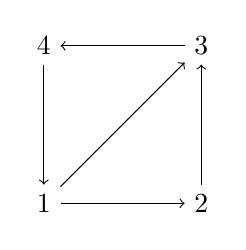
\begin{tikzpicture}
    % a graph with four vertices and five edges
    \node (v1) at (0, 0) {1};
    \node (v2) at (2, 0) {2};
    \node (v3) at (2, 2) {3};
    \node (v4) at (0, 2) {4};
    \draw[->] (v1) -- (v2);
    \draw[->] (v2) -- (v3);
    \draw[->] (v3) -- (v4);
    \draw[->] (v4) -- (v1);
    \draw[->] (v1) -- (v3);
  \end{tikzpicture}
  \tcblower
  A graph with four vertices and five edges.  Vertices are numbered from $1$ to $4$, and
  edges are represented by arrows.  The graph is directed, as the edges have a direction.
\end{figurebox}

A graphical representation of a directed graph with four vertices and five edges is shown
in \cref{fig:graph}.  The vertices are numbered from $1$ to $4$, and the edges are
represented by arrows.

Another common representation of a graph is the adjacency matrix.  An adjacency matrix is
a square matrix $A$ of size $n \times n$, where $n$ is the number of vertices.  The
$i, j$-th entry of the matrix is $1$ if there is an edge from vertex $i$ to vertex $j$,
and $0$ otherwise.  The adjacency matrix of the graph in \cref{fig:graph} is
\[
  A = \begin{pmatrix}
    0 & 1 & 1 & 0 \\
    0 & 0 & 1 & 0 \\
    0 & 0 & 0 & 1 \\
    1 & 0 & 0 & 0
  \end{pmatrix}\text{.}
\]

% \paragraph{Map} A map is a collection of key-value pairs.  The keys are unique, and
% each key is associated with a value.  The keys are used to access the values.

\section{Set theory}

A set is a collection of elements.  The elements of a set can be anything, including
other sets.  The elements of a set are unordered, and each element is unique.  The
most common notation for sets is the curly braces notation, e.g., $\{1, 2, 3\}$.

Some special sets are listed below.

\paragraph{Universe set}  The universe set is the set of all elements in a given context.
It is denoted by $\Omega$.

\paragraph{Empty set}  The empty set is the set with no elements.  It is denoted by
the symbol $\emptyset$.  Depending on the context, it can also be denoted by $\{\}$.

\subsection{Set operations}

The basic operations on sets are union, intersection, difference, and complement.

\paragraph{Union}  The union of two sets $A$ and $B$ is the set of elements that are in
$A$ or $B$.  It is denoted by $A \cup B$.  For example, the union of $\{1, 2, 3\}$ and
$\{3, 4, 5\}$ is $\{1, 2, 3, 4, 5\}$.

\paragraph{Intersection}  The intersection of two sets $A$ and $B$ is the set of elements
that are in both $A$ and $B$.  It is denoted by $A \cap B$.  For example, the intersection
of $\{1, 2, 3\}$ and $\{3, 4, 5\}$ is $\{3\}$.

\paragraph{Difference}  The difference of two sets $A$ and $B$ is the set of elements
that are in $A$ but not in $B$.  It is denoted by $A \setminus B$.  For example, the
difference of $\{1, 2, 3\}$ and $\{3, 4, 5\}$ is $\{1, 2\}$.

\paragraph{Complement}  The complement of a set $A$ is the set of elements that are not
in $A$.  It is denoted by $A^c = \Omega \setminus A$.

\paragraph{Inclusion}  Inclusion is a relation between sets.  A set $A$ is included in a
set $B$ if all elements of $A$ are also elements of $B$.  It is denoted by $A \subseteq B$.

\subsection{Set operations properties}

Union and intersection are commutative, associative, and distributive.  Thus, given sets
$A$, $B$, and $C$, the following statements hold:
\begin{itemize}
  \item \emph{Commutativity:} $A \cup B = B \cup A$ and $A \cap B = B \cap A$;
  \item \emph{Associativity:} $(A \cup B) \cup C = A \cup (B \cup C)$ and $(A \cap B) \cap C = A \cap (B \cap C)$;
  \item \emph{Distributivity:} $A \cup (B \cap C) = (A \cup B) \cap (A \cup C)$ and $A \cap (B \cup C) = (A \cap B) \cup (A \cap C)$.
\end{itemize}

The difference operation can be expressed in terms of union and intersection as
\[
  A \setminus B = A \cap B^c\text{.}
\]

The complement of the union of two sets is the intersection of their complements, i.e.
\[
  (A \cup B)^c = A^c \cap B^c\text{.}
\]
Similarly, the complement of the intersection of two sets is the union of their complements, i.e.
\[
  (A \cap B)^c = A^c \cup B^c\text{.}
\]
This property is known as De Morgan's laws.

In terms of inclusion, given sets $A$, $B$, and $C$, the following statements hold:
\begin{itemize}
  \item \emph{Reflexivity:} $A \subseteq A$;
  \item \emph{Antisymmetry:} $A \subseteq B$ and $B \subseteq A$ if and only if $A = B$;
  \item \emph{Transitivity:} $A \subseteq B$ and $B \subseteq C$ implies $A \subseteq C$.
\end{itemize}

\subsection{Relation to Boolean algebra}

Set operations are closely related to Boolean algebra.  In Boolean algebra, the elements
of a set are either true or false, many times represented by $1$ and $0$, respectively.
The union operation is equivalent to the logical OR operation, expressed by the symbol
$\lor$; and the intersection operation is equivalent to the logical AND operation,
expressed by the symbol $\land$.  The complement operation is equivalent to the logical
NOT operation, expressed by the symbol $\lnot$.

The distributive property of set operations is equivalent to the distributive property of
Boolean algebra.  Important properties like De Morgan's laws also hold in Boolean algebra,
i.e. $\lnot (A \lor B) = \lnot A \land \lnot B$ and $\lnot (A \land B) = \lnot A \lor
\lnot B$.

Boolean algebra is the foundation of digital electronics and computer science.  The
logical operations are implemented in hardware using logic gates, and the logical
operations are used in programming languages to control the flow of a program.

Readers interested in more details about Boolean algebra and Discrete Mathematics
should consult \textcite{Rosen2018}\footfullcite{Rosen2018}.

\section{Linear algebra}

Linear algebra is the branch of mathematics that studies vector spaces and linear
transformations.  It is a fundamental tool in many areas of science and engineering.
The basic objects of linear algebra are vectors and matrices.  A common textbook that
covers the subject in depth is \textcite{Strang2023}\footfullcite{Strang2023}.

\paragraph{Vector}  A vector is an ordered collection of numbers.  It is denoted by a bold
lowercase letter, e.g., $\vec{v} = [v_i]_{i=1,\dots, n}$ is a vector of length $n$.

\paragraph{Matrix}  A matrix is a rectangular collection of numbers.  It is denoted by an
uppercase letter, e.g., $A = (a_{ij})_{i = 1, \dots, n;~j = 1, \dots, m}$ is the matrix
with $n$ rows and $m$ columns.

\paragraph{Tensor}  Tensors are generalizations of vectors and matrices.  A tensor of rank
$k$ is a multidimensional array with $k$ indices.  Scalars are tensors of rank $0$,
vectors are tensors of rank $1$, and matrices are tensors of rank $2$.  Tensors are
commonly used in machine learning and physics.

\subsection{Operations}

The main operations in linear algebra are presented below.

\paragraph{Addition}  The sum of two vectors $\vec{v}$ and $\vec{w}$ is the vector
$\vec{v} + \vec{w}$ whose $i$-th entry is $v_i + w_i$.  The sum of two matrices $A$ and
$B$ is the matrix $A + B$ whose $i, j$-th entry is $a_{ij} + b_{ij}$.  (The same rules apply
to subtraction.)

\paragraph{Scalar multiplication}  The product of a scalar $\alpha$ and a vector $\vec{v}$
is the vector $\alpha \vec{v}$ whose $i$-th entry is $\alpha v_i$.  Similarly, the product of a
scalar $\alpha$ and a matrix $A$ is the matrix $\alpha A$ whose $i, j$-th entry is
$\alpha a_{ij}$.

\paragraph{Dot product}  The dot product of two vectors $\vec{v}$ and $\vec{w}$ is the
scalar $$\vec{v} \cdot \vec{w} = \sum_{i = 1}^n v_i w_i\text{.}$$  The dot product is also called
the inner product.

\paragraph{Matrix multiplication}  The product of two matrices $A$ and $B$ is the matrix
$C = A B$ whose $i, j$-th entry is $$c_{ij} = \sum_{k = 1}^n a_{ik} b_{kj}\text{.}$$
The number of columns of $A$ must be equal to the number of rows of $B$, and the
resulting matrix $C$ has the same number of rows as $A$ and the same number of columns as $B$.
Unless otherwise stated, we consider the vector $\vec{v}$ with length $n$ as a column
matrix, i.e., a matrix with one column and $n$ rows.

\paragraph{Transpose}  The transpose of a matrix $A$ is the matrix $A^T$ whose $i, j$-th
entry is the $j, i$-th entry of $A$.  If $A$ is a square matrix, then $A^T$ is the
matrix obtained by reflecting $A$ along its main diagonal.

\paragraph{Determinant}  The determinant of a square matrix $A$ is a scalar that is a
measure of the (signed) volume of the parallelepiped spanned by the columns of $A$.  It is
denoted by $\det(A)$ or $|A|$.

The determinant is nonzero if and only if the matrix is invertible and the linear map
represented by the matrix is an isomorphism -- i.e., it preserves the dimension of the
vector space.  The determinant of a product of matrices is the product of their
determinants.

Particularly, the determinant of a $2 \times 2$ matrix $\begin{pmatrix} a & b \\ c & d
\end{pmatrix}$ is $$\begin{vmatrix} a & b \\ c & d \end{vmatrix} = ad - bc\text{.}$$

\paragraph{Inverse matrix}  An $n \times n$ matrix $A$ has an inverse $n \times n$ matrix
$A^{-1}$ if
\[
  A A^{-1} = A^{-1} A = I_n\text{,}
\]
where $I_n$ is the $n \times n$ identity matrix, i.e., a matrix whose diagonal entries are
$1$ and all other entries are $0$. If such a matrix exists, $A$ is said to be
\emph{invertible}.  A square matrix that is not invertible is called singular. A square
matrix with entries in a field is singular if and only if its determinant is zero.

To calculate the inverse of a matrix, we can use the formula
\[
  A^{-1} = \frac{1}{\det(A)} \operatorname{adj}(A)\text{,}
\]
where $\operatorname{adj}(A)$ is the adjugate (or adjoint) of $A$, i.e., the transpose of the cofactor matrix
of $A$.

The cofactor of the $i, j$-th entry of a matrix $A$ is the determinant of the matrix
obtained by removing the $i$-th row and the $j$-th column of $A$, multiplied by $(-1)^{i
+ j}$.

In the case of a $2 \times 2$ matrix, the inverse is
\[
  \begin{pmatrix}
    a & b \\
    c & d
  \end{pmatrix}^{-1} = \frac{1}{ad - bc}
  \begin{pmatrix}
    d & -b \\
    -c & a
  \end{pmatrix}\text{.}
\]

\subsection{Systems of linear equations}

A system of linear equations is a collection of linear equations that share their
unknowns.  It is usually written in matrix form as $A \vec{x} = \vec{b}$, where $A$ is a
matrix of constants, $\vec{x}$ is a vector of unknowns, and $\vec{b}$ is a vector of
constants.

The system has a unique solution if and only if the matrix $A$ is invertible.  The
solution is $\vec{x} = A^{-1} \vec{b}$.

% \subsection{Matrix decompositions}
%
% Matrix decompositions are factorizations of matrices into matrices with special
% properties.  They are used to solve linear systems, compute inverses, and compute
% eigenvalues and eigenvectors.
%
% \textcolor{red}{Verify!}
%
% \paragraph{Singular value decomposition} The singular value decomposition (SVD) of a
% matrix $A$ is a factorization of the form
% \begin{equation}
%   \label{eq:svd}
%   A = U \Sigma V^T\text{,}
% \end{equation}
% where $U$ and $V$ are orthogonal matrices and $\Sigma$ is a diagonal
% matrix with non-negative real numbers on the diagonal.  The singular values are the
% diagonal entries of $\Sigma$.
%
% \paragraph{Eigenvalue decomposition}  The eigenvalue decomposition of a matrix $A$
% is a factorization of the form
% \begin{equation}
%   \label{eq:eigdec}
%   A = Q \Lambda Q^{-1}\text{,}
% \end{equation}
% where $Q$ is a square matrix whose columns are the eigenvectors of $A$, and
% $\Lambda$ is a diagonal matrix whose diagonal entries are the eigenvalues of
% $A$.
%
% \paragraph{Cholesky decomposition}  The Cholesky decomposition of a positive-definite
% matrix $A$ is a factorization of the form
% \begin{equation}
%   \label{eq:chol}
%   A = L L^T\text{,}
% \end{equation}
% where $L$ is a lower triangular matrix with real and positive diagonal entries.
%
% \paragraph{QR decomposition}  The QR decomposition of a matrix $A$ is a
% factorization of the form
% \begin{equation}
%   \label{eq:qr}
%   A = Q R\text{,}
% \end{equation}
% where $Q$ is an orthogonal matrix and $R$ is an upper triangular matrix.
%
% \paragraph{LU decomposition}  The LU decomposition of a square matrix $A$ is a
% factorization of the form
% \begin{equation}
%   \label{eq:lu}
%   A = L U\text{,}
% \end{equation}
% where $L$ is a lower triangular matrix with unit diagonal entries and $U$ is
% an upper triangular matrix.

\subsection{Eigenvalues and eigenvectors}

An eigenvalue of an $n \times n$ square matrix $A$ is a scalar $\lambda$ such that there exists a
non-zero vector $\vec{v}$ satisfying
\begin{equation}
  \label{eq:eig}
  A \vec{v} = \lambda \vec{v}\text{.}
\end{equation}
The vector $\vec{v}$ is called an eigenvector of $A$ corresponding to $\lambda$.

The eigenvalues of a matrix are the roots of its characteristic polynomial, i.e., the
roots of the polynomial $\det(A - \lambda I_n) = 0$, where $I_n$ is the $n \times n$ identity matrix.

\section{Probability}

Probability is the branch of mathematics that studies the likelihood of events.  It is
used to model uncertainty and randomness.  The basic objects of probability are events
and random variables.

For a comprehensive material about probability theory, the reader is referred to
\textcite{Ross2019}\footfullcite{Ross2019} and \textcite{Ross2023}\footfullcite{Ross2023}.

\subsection{Axioms of probability and main concepts}

The Kolmogorov axioms of probability are the foundation of probability theory.
They are
\begin{enumerate}
  \item The probability of an event $A$ is a non-negative real number, i.e. $\Prob(A) \geq 0$;
  \item The probability of the sample space\footnote{The set of all possible
    events.}, denoted by $\Omega$, is one, i.e. $\Prob(\Omega) = 1$; and
  \item The probability of the union of disjoint events, $A \cap B = \emptyset$, is
    the sum of the probabilities of the events, i.e. $\Prob(A \cup B) = \Prob(A) + \Prob(B)$.
\end{enumerate}

\paragraph{Sum rule}
A particular consequence of the third axiom is the addition law of probability.
If $A$ and $B$ are not disjoint, then
\begin{equation*}
  \Prob(A \cup B) = \Prob(A) + \Prob(B) - \Prob(A \cap B)\text{.}
\end{equation*}

\paragraph{Joint probability}

The joint probability of two events $A$ and $B$ is the probability that both events
occur.  It is denoted by $\Prob(A, B) = \Prob(A \cap B)$.

\paragraph{Law of total probability}

The law of total probability states that if $B_1, \dots, B_n$ are disjoint events
such that $\cup_{i = 1}^n B_i = \Omega$, then for any event $A$, we have that
$$\Prob(A) = \sum_{i = 1}^n \Prob(A, B_i)\text{.}$$

\paragraph{Conditional probability}

The conditional probability of an event $A$ given an event $B$ is the probability
that $A$ occurs given that $B$ occurs.  It is denoted by $\Prob(A \mid B)$.

\paragraph{Independence}

Two events $A$ and $B$ are independent if the probability of $A$ given $B$ is the
same as the probability of $A$, i.e., $\Prob(A \mid B) = \Prob(A)$.  It is equivalent to
$\Prob(A, B) = \Prob(A) \cdot \Prob(B)$.

\paragraph{Bayes' rule}

Bayes' rule is a formula that relates the conditional probability of an event $A$
given an event $B$ to the conditional probability of $B$ given $A$.  It is
\begin{equation}
  \label{eq:bayes}
  \Prob(A \mid B) = \frac{\Prob(B \mid A) \cdot \Prob(A)}{\Prob(B)}\text{.}
\end{equation}
Bayes' rule is one of the most important formulas in probability theory and is used
in many areas of science and engineering.  Particularly, for data science, it is
used in Bayesian statistics and machine learning.

\subsection{Random variables}

A random variable is a function that maps the sample space $\Omega$ to the real
numbers.  It is denoted by a capital letter, e.g., $X$.

Formally, let $X : \Omega \rightarrow E$ be a random variable.  The
probability that $X$ takes on a value in a set $A \subseteq E$ is
\begin{equation}
  \label{eq:rv}
  \Prob(X \in A) = \Prob(\{\omega \in \Omega : X(\omega) \in A\})\text{.}
\end{equation}

If $E = \mathbb{R}$, then $X$ is a continuous random variable.  If $E = \mathbb{Z}$,
then $X$ is a discrete random variable.  The random variable $X$ is said to follow
a certain probability distribution $P$ --- denoted by $X \sim P$ --- given by its
probability mass function or probability density function --- see below.

\paragraph{Probability mass function}

The \gls{pmf} of a discrete random variable $X$ is the
function $p_X : \mathbb{Z} \rightarrow [0, 1]$ defined by
\begin{equation}
  \label{eq:pmf}
  p_X(x) = \Prob(X = x)\text{.}
\end{equation}

\paragraph{Probability density function}

We call \gls{pdf} of a continuous random variable $X$ the
function $f_X : \mathbb{R} \rightarrow [0, \infty)$ defined by
\begin{equation}
  \label{eq:pdf}
  \Prob(a \leq X \leq b) = \int_a^b f_X(x) dx\text{.}
\end{equation}

\paragraph{Cumulative distribution function}

Similarly, the \gls{cdf} of a random variable $X$ is the function
$F_X : \mathbb{R} \rightarrow [0, 1]$ defined by
\begin{equation}
  \label{eq:cdf}
  F_X(x) = \Prob(X \leq x)\text{.}
\end{equation}

\subsection{Expectation and moments}

Expectation is a measure of the average value of a random variable.  Moments are
measures of the shape of a probability distribution.

\paragraph{Expectation}  The expectation of a random variable $X$ is the average
value of $X$.  It is denoted by $\E[X]$.  By definition, it is
\begin{equation*}
  \E[X] = \sum_{x} x \cdot p_X(x)\text{,}
\end{equation*}
if $X$ is discrete, or
\begin{equation*}
  \E[X] = \int_{-\infty}^{\infty} x \cdot f_X(x) dx\text{,}
\end{equation*}
if $X$ is continuous.

The main properties of expectation are listed below.

The expectation operator is linear.  Given two random variables $X$ and $Y$ and a real
number $c$, we have
\begin{equation*}
  \E[c X] = c \E[X]\text{,}
\end{equation*}
\begin{equation*}
  \E[X + c] = \E[X] + c\text{,}
\end{equation*}
and
\begin{equation*}
  \E[X + Y] = \E[X] + \E[Y]\text{.}
\end{equation*}

Under a more general setting, given a function $g : \mathbb{R} \rightarrow \mathbb{R}$,
the expectation of $g(X)$ is
\begin{equation*}
  \E[g(X)] = \sum_{x} g(x) \cdot p_X(x)\text{,}
\end{equation*}
if $X$ is discrete, or
\begin{equation*}
  \E[g(X)] = \int_{-\infty}^{\infty} g(x) \cdot f_X(x) dx\text{,}
\end{equation*}
if $X$ is continuous.

\paragraph{Variance}  The variance of a random variable $X$ is a measure of how
spread out the values of $X$ are.  It is denoted by $\Var(X)$.  By definition, it is
\begin{equation}
  \label{eq:variance}
  \Var(X) = \E\!\left[\left(X - \E[X]\right)^2\right]\text{.}
\end{equation}

Note that, as a consequence, the expectation of $X^2$ --- called the second moment --- is
\[
  \E[X^2] = \Var(X) + \E[X]^2\text{,}
\]
since
\begin{align*}
  \Var(X)
    &= \E\!\left[\left(X - \E[X]\right)^2\right] \\
    &= \E\!\left[X^2 - 2 X \E[X] + \E[X]^2\right] \\
    &= \E[X^2] - 2 \E[X] \E[X] + \E[X]^2 \\
    &= \E[X^2] - \E[X]^2\text{.}
\end{align*}

Higher moments are defined similarly.  The $k$-th moment of $X$ is
\begin{equation*}
  \E[X^k] = \sum_{x} x^k \cdot p_X(x)\text{,}
\end{equation*}
if $X$ is discrete, or
\begin{equation*}
  \E[X^k] = \int_{-\infty}^{\infty} x^k \cdot f_X(x) dx\text{,}
\end{equation*}
if $X$ is continuous.

\paragraph{Sample mean}  The sample mean is the average of a sample of random variables.
Given a sample $X_1, \dots, X_n$ such that $X_i \sim X$ for all $i$, the sample mean is
\begin{equation*}
  \bar{X} = \frac{1}{n} \sum_{i = 1}^n X_i\text{.}
\end{equation*}

\paragraph{Law of large numbers}  The law of large numbers states that the average of
a large number of independent and identically distributed (i.i.d.) random variables converges
to the expectation of the random variable.  Mathematically,
\begin{equation*}
  \lim_{n \rightarrow \infty} \frac{1}{n} \sum_{i = 1}^n X_i = \E[X]\text{,}
\end{equation*}
given $X_i \sim X$ for all $i$.

\paragraph{Sample variance}  The sample variance is a measure of how spread out the
values of a sample are.  Given a sample $X_1, \dots, X_n$ such that $X_i \sim X$ for all
$i$, the sample variance is
\begin{equation*}
  S^2 = \frac{1}{n - 1} \sum_{i = 1}^n (X_i - \bar{X})^2\text{.}
\end{equation*}
Note that the denominator is $n - 1$ instead of $n$ to correct the bias of the sample
variance.

\paragraph{Sample standard deviation}  The sample standard deviation is the square root
of the sample variance, i.e., $S = \sqrt{S^2}$.

\paragraph{Sample skewness}  The skewness is a measure of the asymmetry of a probability
distribution.  The sample skewness is based on the third moment of the sample.  Given a
sample $X_1, \dots, X_n$ such that $X_i \sim X$ for all $i$, the sample skewness is
\begin{equation*}
  \text{Skewness} = \frac{\frac{1}{n} \sum_{i = 1}^n (X_i - \bar{X})^3}{S^3}\text{.}
\end{equation*}
Skewness is zero for a symmetric distribution.  Otherwise, it is positive for a right-skewed distribution,
and negative for a left-skewed distribution.

\paragraph{Sample kurtosis}  The kurtosis is a measure of the tailedness of a probability
distribution.  The sample kurtosis is based on the fourth moment of the sample.  Given a
sample $X_1, \dots, X_n$ such that $X_i \sim X$ for all $i$, the sample kurtosis is
\begin{equation*}
  \text{Kurtosis} = \frac{\frac{1}{n} \sum_{i = 1}^n (X_i - \bar{X})^4}{S^4} - 3\text{.}
\end{equation*}
Kurtosis is positive if the tails are heavier than a normal distribution, and negative if
the tails are lighter.

\subsection{Common probability distributions}

Several phenomena in nature and society can be modeled as random variables.  Some
distributions are frequently used to model these phenomena.  The main ones are
listed below.

\paragraph{Bernoulli distribution}  The Bernoulli distribution is a discrete
distribution with two possible outcomes, usually called success and failure.  It is
parametrized by a single parameter $p \in [0, 1]$, which is the probability of
success.  It is denoted by $\text{Bern}(p)$.

The expected value of $X \sim \text{Bern}(p)$ is $\E[X] = p$, and the variance is
$\Var(X) = p(1 - p)$.

\paragraph{Poisson distribution}  The Poisson distribution is a discrete distribution
that models the number of events occurring in a fixed interval of time or space.  It is
parametrized by a single parameter $\lambda > 0$, which is the average number of events
in the interval.  It is denoted by $\text{Poisson}(\lambda)$.

The probability mass function of $X \sim \text{Poisson}(\lambda)$ is
\begin{equation}
  \label{eq:poisson}
  p_X(x) = \frac{e^{-\lambda} \lambda^x}{x!}\text{.}
\end{equation}

The expected value of $X \sim \text{Poisson}(\lambda)$ is $\E[X] = \lambda$, and the
variance is $\Var(X) = \lambda$.

\paragraph{Normal distribution} The normal distribution is a continuous distribution
with a bell-shaped density.  It is parametrized by two parameters, the mean $\mu \in
\mathbb{R}$ and the standard deviation $\sigma > 0$.  It is denoted by
$\mathcal{N}(\mu, \sigma^2)$.

The special case where $\mu = 0$ and $\sigma = 1$ is called the standard normal
distribution.  It is denoted by $\mathcal{N}(0, 1)$.

The probability density function of $X \sim \mathcal{N}(\mu, \sigma^2)$ is
\begin{equation}
  \label{eq:normal}
  f_X(x) = \frac{1}{\sqrt{2 \pi \sigma^2}} \exp\left(-\frac{(x - \mu)^2}{2 \sigma^2}\right)\text{.}
\end{equation}

The expected value of $X \sim \mathcal{N}(\mu, \sigma^2)$ is $\E[X] = \mu$, and the
variance is $\Var(X) = \sigma^2$.

\paragraph{Central limit theorem}  The central limit theorem states that the normalized
version of the sample mean converges to a standard normal distribution\footnote{This
statement of the central limit theorem is known as the Lindeberg-Levy CLT.  There are
other versions of the central limit theorem, some more general and some more
restrictive.}. Given $X_1, \dots, X_n$ i.i.d. random variables with mean $\mu$ and finite
variance $\sigma^2 < \infty$,
\begin{equation*}
  \sqrt{n} (\bar{X} - \mu) \sim \mathcal{N}(0, \sigma^2)\text{,}
\end{equation*}
as $n \rightarrow \infty$.  In other words, for a large enough $n$, the distribution of
the sample mean gets closer\footnote{Formally, this is called convergence in distribution,
refer to \fullcite{Billingsley1995} for more details.} to a normal distribution with mean
$\mu$ and variance $\sigma^2/n$.

The central limit theorem is one of the most important results in probability theory and
statistics.  Its implications are fundamental in many areas of science and engineering.

\paragraph{T distribution} The T distribution is a continuous distribution with a
bell-shaped density.  It is parametrized by a single parameter $\nu > 0$, called the
degrees of freedom.  It is denoted by $\mathcal{T}(\nu)$.

% The probability density function of $X \sim \mathcal{T}(\nu)$ is
% \begin{equation}
%   \label{eq:t}
%   f_X(x) = \frac{\Gamma\left(\frac{\nu + 1}{2}\right)}{\sqrt{\nu \pi} \Gamma\left(\frac{\nu}{2}\right)}
%   \left(1 + \frac{x^2}{\nu}\right)^{-\frac{\nu + 1}{2}}\text{.}
% \end{equation}

The T distribution generalizes to the three-parameter location-scale t distribution
$\mathcal{T}(\mu, \sigma^2, \nu)$, where $\mu$ is the location parameter and $\sigma$ is
the scale parameter.  Thus, given $X \sim \mathcal{T}(\nu)$, we have that
$\mu + \sigma X \sim \mathcal{T}(\mu, \sigma^2, \nu)$.

Note that $$\lim_{\nu \rightarrow \infty} \mathcal{T}(\nu) = \mathcal{N}(0, 1)\text{.}$$
Thus, the T distribution converges to the standard normal distribution as the degrees of
freedom go to infinity.

\paragraph{Gamma distribution} The Gamma distribution is a continuous distribution with a
right-skewed density.  It is parametrized by two parameters, the shape parameter $\alpha
> 0$ and the rate parameter $\beta > 0$.  It is denoted by $\text{Gamma}(\alpha, \beta)$.

The probability density function of $X \sim \text{Gamma}(\alpha, \beta)$ is
\begin{equation}
  \label{eq:gamma}
  f_X(x) = \frac{\beta^\alpha x^{\alpha - 1} e^{-\beta x}}{\Gamma(\alpha)}\text{,}
\end{equation}
where $\Gamma(\alpha)$ is the gamma function, defined by
\begin{equation}
  \label{eq:gammaf}
  \Gamma(\alpha) = \int_0^\infty t^{\alpha - 1} e^{-t} dt\text{.}
\end{equation}

In Bayesian analysis, the Gamma distribution is commonly used as a conjugate prior.
A conjugate prior is a prior distribution that, when combined with the likelihood,
results in a posterior distribution that is of the same family as the prior.

\subsection{Permutations and combinations}

For the sake of reference, we present some definitions and formulas from
combinatorics. Combinatorics is the branch of mathematics that studies the counting of
objects.

\paragraph{Factorial}  The factorial of a non-negative integer $n$ is the product of all
positive integers up to $n$.  It is denoted by
\[
  n! = n \cdot (n - 1) \cdot \text\dots \cdot 2 \cdot 1\text{.}
\]
By definition, $0! = 1$.

\paragraph{Permutation}  A permutation is an arrangement of a set of elements.  The
number of permutations of $n$ elements is $n!$.  Permutations are used in combinatorics
to count the number of ways to arrange a set of elements.

\paragraph{Combination}  A combination is a selection of a subset of elements from a set.
The number of combinations of $k$ elements from a set of $n$ elements is $$\binom{n}{k} =
\frac{n!}{k!(n - k)!}\text{.}$$  Combinations are used in combinatorics to count the
number of ways to select a subset of elements from a set.  The binomial coefficient
is also called a choose function, and is read as ``$n$ choose $k$''.

% \section{Optimization}
%
% Optimization is the process of finding the best solution to a problem.  The best
% solution is called the (global) optimum.  The optimum can be a maximum or a minimum.
% Sometimes, we are interested in finding a local optimum, which is the best solution
% in a neighborhood of the current solution.  Also, we might be interested in finding
% a solution that is good enough, i.e. a solution that is close to the optimum.
% In this case, we use heuristics to search in the solution space.
%
% \subsection{Minimization of convex functions}
%
% Maybe the simplest case of optimization is the minimization of a convex function.
% A function $f : \mathbb{R}^n \rightarrow \mathbb{R}$ is convex if for any two points
% $\vec{v}$ and $\vec{w}$ in the domain of $f$, the line segment connecting them lies
% above the graph of $f$.  Mathematically, it means that
% $$f(t\vec{v} + (1 - t) \vec{w}) \leq t f(\vec{v}) + (1 - t) f(\vec{w})$$ for all $t \in [0, 1]$.
%
% \subsection{Gradient descent}
%
% Gradient descent is an iterative algorithm for finding the minimum of a function.
% It is based on the observation that the gradient of a function points in the
% direction of the steepest descent.  The algorithm is
% \begin{equation}
%   \label{eq:gd}
%   \vec{w}(t + 1) = \vec{w}(t) - \alpha \nabla f(\vec{w}(t))\text{,}
% \end{equation}
%
% \subsection{Constraint optimization}
%
% Techniques like Lagrange multipliers, penalty methods, and barrier methods are used to
% handle constrained optimization problems in data science.
%
% \subsection{Convex optimization}
%
% Convex optimization problems, where the objective function and the constraints are convex,
% have efficient algorithms that guarantee global optimality.

% \subsection{Gradient descent algorithm}
%
% Let $f(\vec{w})$, $f : \mathbb{R}^n \rightarrow \mathbb{R}$, be an objective function that
% we are trying to minimize.  We know that
% $f$ is convex, of class $\mathcal{C}^2$, and its gradient $\nabla f$ is Lipschitz continuous with Lipschitz
% constant $L > 0$.
%
% We want to show that $\lim_{t\rightarrow\infty} f(\vec{w}(t)) = f^{*}$ where $f^{*}$
% is the global minimum of $f$ and $$\vec{w}(t+1) = \vec{w}(t) - \alpha \nabla f(\vec{w}(t))\mbox{,}$$
% for any initial condition $\vec{w}(0)$ and $0 < \alpha \leq \frac{1}{L}$.
%
% Convexity implies that for any two points $\vec{v}$ and $\vec{w}$ in the domain of
% $f$, the line segment connecting them lies above the graph of $f$.  Mathematically, it
% means that $$f(t\vec{v} + (1 - t) \vec{w}) \leq t f(\vec{v}) + (1 - t)
% f(\vec{w})$$ for all $t \in [0, 1]$.
%
% The Lipschitz continuity condition means that the gradient of $f(\vec{w})$ does not change too rapidly.
% Formally, $$\left\|\nabla f(\vec{v}) - \nabla f(\vec{w})\right\| \leq L \|\vec{v} - \vec{w}\|\mbox{,}$$
% for all $\vec{v}$ and $\vec{w}$ in the domain of $f$.  This is a rather weak
% assumption, and it means that the gradient can not change arbitrarily fast.
%
% Since $f$ is convex and twice differentiable, its Hessian is a positive semidefinite
% matrix, and thus its norm is its largest eigenvalue.
%
% A consequence of the Lipschitz continuity for a $\mathcal{C}^2$ function $f$ is that for
% any $\vec{v}$ and $\vec{w}$, we have that
% \begin{equation}
%   \label{eq:lcg1}
%   \vec{v}^T \nabla^2 f(w) \vec{v} \leq L \|v\|^2\text{.}
% \end{equation}
% It means that the eigenvalues of the Hessian are bounded above by $L$.
%
% \paragraph{Descent lemma.}  For $f$, a the multivariate Taylor expansion is that
% $$f(w) = f(v)$$

% vim: spell spelllang=en

\chapter{Topics on learning machines}
\label[appendix]{chap:learning-machines}
\glsresetall


\chapterprecishere{Oh, the depth of the riches and wisdom and knowledge of God! How
  unsearchable are his judgments and how inscrutable his ways!
  \par\raggedleft--- \textup{Romans 11:33} (ESV)}

This appendix is under construction.  Topics like the kernel trick, back-propagation, and
other machine learning algorithms will be discussed here.

{}
\clearpage

\section{Multi-layer perceptron}
\label{sec:mlp}

The \gls{mlp} is a non-linear classifier that generates a set of hyperplanes
that separates the classes.  In order to simplify understanding, consider
that the activation function of the hidden layer is the discrete step function
\begin{equation*}
  \sigma(x) = \begin{cases}
    1 & \text{if } x > 0 \\
    0 & \text{otherwise.}
  \end{cases}
\end{equation*}
A model with two neurons in the hidden layer (effectively the combination of three
perceptrons) is
\begin{multline*}
  f(x_1, x_2; \theta = \left\{ \vec{w}^{(1)}, \vec{w}^{(2)}, \vec{w}^{(3)} \right\}) = \\
  \sigma\left(
    \vec{w}^{(3)} \cdot \left[1, \sigma(\vec{w}^{(1)} \cdot \vec{x}), \sigma(\vec{w}^{(2)} \cdot \vec{x})\right]
  \right)\text{.}
\end{multline*}

The parameters $\vec{w}^{(1)}$ and $\vec{w}^{(2)}$ represent the hyperplanes that separate
the classes in the hidden layer, and $\vec{w}^{(3)}$ represents how the hyperplanes are
combined to generate the output.  If we set weights $\vec{w}^{(1)} = [-0.5, 1, -1]$ (like the
perceptron in the previous example) and $\vec{w}^{(2)} = [-0.5, -1, 1]$, we use the third neuron
to combine the results of the first two neurons.  This way, a possible solution for the
XOR problem is setting $\vec{w}^{(3)} = [0, 1, 1]$.

\begin{figurebox}[label=fig:mlp]{MLP class boundaries for the XOR problem.}
  \centering
  \begin{tikzpicture}
    \begin{axis}[
        axis x line=bottom,
        axis y line=left,
        xlabel={$x_1$},
        ylabel={$x_2$},
        width=0.6\textwidth,
        height=0.6\textwidth,
        xtick={0, 1},
        ytick={0, 1},
        xmin=-0.5, xmax=1.5,
        ymin=-0.5, ymax=1.5,
      ]
      \addplot+[only marks, mark=+, color=black, mark size=3pt] coordinates {
        (0, 1) (1, 0)
      };
      \addplot+[only marks, mark=-, color=black, mark size=3pt] coordinates {
        (0, 0) (1, 1)
      };
      \addplot+[domain=0:1.5, mark=none, black, thick] {-0.5 + x};
      \addplot+[domain=-0.5:1.5, mark=none, black, thick] {0.5 + x};
    \end{axis}
  \end{tikzpicture}
  \tcblower
  \Gls{mlp} with two neurons in the hidden layer generates two linear hyperplanes that
  separate the classes, effectively solving the XOR problem.
\end{figurebox}

\begin{tablebox}[label=tab:xor-mlp]{Truth table for the predictions of the MLP.}
  \centering
  \rowcolors{2}{black!10!white}{}
  \begin{tabular}{ccc|cccc}
    \toprule
    $x_1$ & $x_2$ & $y$ & \nth{1} neuron & \nth{2} neuron & $\hat{y}$ \\
    \midrule
    0 & 0 & 0 & 0 & 0 & 0 \\
    0 & 1 & 1 & 0 & 1 & 1 \\
    1 & 0 & 1 & 1 & 0 & 1 \\
    1 & 1 & 0 & 0 & 0 & 0 \\
    \bottomrule
  \end{tabular}
  \tcblower
  Predictions of the \gls{mlp} for the XOR problem.  The output of the \nth{1} and \nth{2}
  neurons are hyperplanes that separate the classes in the hidden layer, which are
  combined by the \nth{3} neuron to generate the correct output.
\end{tablebox}

\Cref{fig:mlp,tab:xor-mlp} show the class boundaries and the predictions of the MLP for
the XOR problem.

Note that there are many possible solutions for the XOR problem using the MLP.
Learning strategies like back-propagation are used to find the optimal parameters for
the model and regularization techniques, like $l_1$ and $l_2$ regularization, are used to
prevent overfitting.

% TODO: backpropagation and regularization
% TODO: talk about deep learning

Deep learning is the study of neural networks with many layers.  The idea is to use many
layers to learn not only the boundaries that separate the classes (or the function that
maps inputs and outputs) but also the features that are relevant to the problem.
A complete discussion of deep learning can be found in
\textcite{Goodfellow2016}\footfullcite{Goodfellow2016}.

\clearpage
\section{Decision trees}

The decision tree is a non-linear classifier that generates a set of hyperplanes that
are orthogonal to the axes.  Consider the decision tree in \cref{fig:tree-and}.

\begin{figurebox}[label=fig:tree-and]{Decision tree representation.}
  \centering
  \begin{tikzpicture}
    \node[decision] (x1) at (0, 0) {$x_1$};
    \node[block] (n1) at (-2, -1.5) {$\hat{y} = 0$};
    \node[decision] (x2) at (2, -1.5) {$x_2$};
    \node[block] (n2) at (0, -3) {$\hat{y} = 0$};
    \node[block] (p) at (4, -3) {$\hat{y} = 1$};

    \draw (x1) -| (n1) node [midway, above] {$\leq 0.5$};
    \draw (x1) -| (x2) node [midway, above] {$>0.5$};
    \draw (x2) -| (n2) node [midway, above] {$\leq 0.5$};
    \draw (x2) -| (p) node [midway, above] {$>0.5$};
  \end{tikzpicture}
  \tcblower
  The decision tree that solves the AND problem.
\end{figurebox}

\begin{figurebox}[label=fig:tree-bias]{Decision tree spatial representation.}
  \centering
  \begin{tikzpicture}
    \begin{axis}[
        axis x line=bottom,
        axis y line=left,
        xlabel={$x_1$},
        ylabel={$x_2$},
        width=0.6\textwidth,
        height=0.6\textwidth,
        xtick={0, 1},
        ytick={0, 1},
        xmin=-0.5, xmax=1.5,
        ymin=-0.5, ymax=1.5,
      ]
      \addplot+[only marks, mark=+, black, mark size=3pt] coordinates {
        (1, 1)
      };
      \addplot+[only marks, mark=-, black, mark size=3pt] coordinates {
        (0, 0) (0, 1) (1, 0)
      };
      \addplot+[domain=0.5:1.5, mark=none, black, thick] {0.5};
      \addplot+[mark=none, black, thick] coordinates {(0.5, -0.5) (0.5, 1.5)};
    \end{axis}
  \end{tikzpicture}
  \tcblower
  Decision trees assume that the classes can be separated with
  hyperplanes orthogonal to the axes.
\end{figurebox}

The spatial representation of the decision tree is shown in \cref{fig:tree-bias}.
Decision trees are a type of classifier that generates a set of hyperplanes orthogonal to the axes.

Decision trees are nonparametric models, one can easily increase the depth of the tree to
fit the data, generating as many hyperplanes as necessary to separate the classes.
Training a decision tree with a large depth can lead to overfitting, so it is important to
use techniques like depth limit and pruning to prevent this from happening.

% \subsection{$k$-nearest neighbors learning bias}
%
% The $k$-nearest neighbors ($k$-NN) is a non-linear nonparametric classifier that
% generate arbitrarily complex decision boundaries by ``memoring'' the training data.
% The behavior of the boundaries depends on the value of $k$ and the distance metric one
% uses to find the nearest neighbors of a point.
%
% \begin{figurebox}[label=fig:1nn-bias]{1-NN learning bias.}
%   \centering
%   \begin{tikzpicture}
%     \begin{axis}[
%         axis x line=bottom,
%         axis y line=left,
%         xlabel={$x_1$},
%         ylabel={$x_2$},
%         width=0.6\textwidth,
%         height=0.6\textwidth,
%         xtick={0, 1},
%         ytick={0, 1},
%         grid=both,
%         xmin=-0.5, xmax=1.5,
%         ymin=-0.5, ymax=1.5,
%       ]
%       \addplot+[only marks, mark=+, mark size=3pt] coordinates {
%         (1, 1)
%       };
%       \addplot+[only marks, mark=*, mark size=3pt] coordinates {
%         (0, 0) (0, 1) (1, 0)
%       };
%       \addplot+[domain=0.5:1.5, mark=none, black, thick] {0.5};
%       \addplot+[mark=none, black, thick] coordinates {(0.5, 0.5) (0.5, 1.5)};
%     \end{axis}
%   \end{tikzpicture}
%   \tcblower
%   In this particular case, the 1-NN boundaries match the decision tree boundaries.
% \end{figurebox}
%
% As $k$ increases the boundaries become smoother:
% \href{https://images.squarespace-cdn.com/content/v1/5d782753c70af105c29a9b14/1580261947016-XODPUVKWPGGMJJMAXSNF/Screen+Shot+2020-01-28+at+8.38.55+PM.png}{example}.
%
% See illustration: \href{https://scikit-learn.org/stable/auto_examples/classification/plot_classifier_comparison.html}{here}.

% vim: spell spelllang=en


\printglossary

\printbibliography[heading=bibintoc]

\end{document}
